%\documentclass[makeidx,envcountchap,graybox,deutsch,ngerman,sectrefs]{svmono}
%\documentclass[envcountchap,graybox,deutsch,sectrefs]{svmono}
%%%%% eigene tempor�re Abk�rzungsliste, f�r die Zeit, bis einheitliche Schreibungen bestehen
\usepackage{tempshort}
%%  Von Springer empfohlene Pakete %% 
%%\documentclass[envcountsect,graybox,deutsch,sectrefs]{svmono}
\usepackage{chapterbib}
\usepackage{type1cm}
\usepackage[ansinew]{inputenc}
\usepackage{babel}
\usepackage[pdftex]{graphicx} %PDF-Vektorgrafiken einbinden
\usepackage{newtxtext} %Typischer Springer-Font
\usepackage{newtxmath}
\usepackage{multicol}
\usepackage[bottom]{footmisc} %Platziert alle Fu�noten unten  
\usepackage[nobreak]{cite}
%\usepackage{biblatex}
\usepackage{cancel}
\usepackage[absolute]{textpos}
\usepackage{graphicx}
\usepackage{pdfpages}

%\usepackage{floatrow}
%\usepackage{mwe}
\usepackage[figuresright]{rotating}
\usepackage{bigints}
\let\laplace\relax  % Vermeidung der Fehlermeldung "\laplace already defined."
\usepackage{trfsigns}
\usepackage{amsmath}
\usepackage{tabulary}
\usepackage{tabularx}

%%  Eigene Pakete %%
\usepackage{adjustbox}
\usepackage{wasysym}
\usepackage{gensymb}
\usepackage{float}
\usepackage{caption}
\usepackage[left=5cm,right=4cm,top=3cm,bottom=4cm,includeheadfoot]{geometry}

%\usepackage{wasysym}
%\usepackage{bigints}
%\usepackage{esint}
%\usepackage{relsize,exscale}

\usepackage{mathtools}   % Vermeidung der Fehlermeldung "Undefined control sequence \coloneqq."


% header and footer
\usepackage{fancyhdr}
\pagestyle{fancy}
\fancyhead[LE,RO]\thepage
\renewcommand{\sectionmark}[1]{\markright{\thesection.\ #1}}
%\fancyhead[LO]{\nouppercase\leftmark}
%\fancyhead[RE]{\nouppercase\rightmark}
\fancyhead[LO]{\nouppercase\rightmark}
\fancyhead[RE]{\nouppercase\leftmark}
\fancyfoot{}
% svmono hat offenbar irgendwas merkw�rdig definiert, darum mu� hier verbreitert werden
%\addtolength\headwidth{25pt}
\setlength{\headheight}{25pt}

%% Units
\usepackage{siunitx}
\sisetup{
  locale = US,
  per-mode = reciprocal, %symbol, % | reciprocal | fraction | ?
  exponent-product = \cdot,
  separate-uncertainty,
  %exponent-to-prefix,
  %prefixes-as-symbols = false,
  %list-units = brackets,% | single | repeat
  %range-units = brackets,% | single | repeat
  %multi-part-units = brackets,% | single | repeat
}
\usepackage{chngcntr}
\usepackage{booktabs}
\usepackage{slashed}
\usepackage{listings}
\usepackage{color} %red, green, blue, yellow, cyan, magenta, black, white
%\usepackage{color} %Einfache Farbendefinition -> von Graybox-Option ben�tigt
\usepackage{multirow}
\usepackage{longtable} %Tabellen �ber mehrere Seiten hinweg
\usepackage{framed} % von Graybox-Option ben�tigt
\usepackage[shortlabels]{enumitem} %Erweiterte Aufz�hloptionen
\usepackage{array}
\usepackage[xindy]{imakeidx} %Wortindex und Personenindex erstellen

\usepackage[hyphens]{url}
%\usepackage[breaklinks,colorlinks=true,linkcolor=black,urlcolor=blue,citecolor=black,filecolor=green,hyperfootnotes=false]{hyperref}
\usepackage[                                    %Hyperref erstellt ein Bookmark/Lesezeichen im PDF. siehe https://www.namsu.de/Extra/pakete/Hyperref.html
bookmarksopen=true,															%Das Lesezeichen ist ge�ffnet beim �ffnen der PDF.
bookmarksnumbered=true,                         %Zahlen werden im Bookmark angezeigt.   
plainpages=false,
pdfpagelabels,
colorlinks=true,                                %Links werden farbig dargestellt.
linkcolor=black, citecolor=black, urlcolor=cyan %Farben definieren.
]{hyperref}                                     %Sollte als letztes eingebunden werden, da es sehr viele Verweise und �nderungen erzeugt. Das Packet ist sehr stark, aber auch umfangreich ist. 

%\usepackage[breaklinks,colorlinks=true,linkcolor=black,urlcolor=blue,citecolor=black,filecolor=green,hyperfootnotes=false]{hyperref}
%\usepackage[breaklinks,colorlinks=true,linkcolor=black,urlcolor=blue,citecolor=black,filecolor=green,hyperfootnotes=false
            %pdftex,
            %pdfauthor={Kaschke, Cartarius},
            %pdftitle={Finger�bungen der Physik}
            %pdfsubject={Ein Repetitorium und �bungsbuch zu im Studium wenig behandelten Kapiteln der Physik mit ausf�hrlich behandelten Problemen und MATLAB-Programmen},
            %pdfkeywords={Physik, Mechanik}
            %]{hyperref}
\pdfminorversion=5

\usepackage{hypcap}
\usepackage[record,section=section,stylemods={mcols},automake]{glossaries-extra}
\usepackage{glossary-longextra}
%\usepackage{glossary-bookindex}
%\makeindex
\setglossarystyle{long-name-sym-desc-loc}
\setabbreviationstyle[acronym]{long-short}

\definecolor{killA}{rgb}{.7,.3,.3}
\newcommand\killA[1]{\bgroup\color{killA}{\cancel{#1}}\egroup}
\newcommand\killB[1]{\bgroup\color{cyan!30!black}{\cancel{#1}}\egroup}

% typographisch korrekte Abk�rzungen (needs to be loaded after hyperref)
\usepackage{abbrev}
\newglossary*{bew}{Glossar}
\newglossary*{hm}{Glossar}
\newglossary*{adyn}{Glossar}
\newglossary*{kontmech}{Glossar}
\newglossary*{aero}{Glossar}
\newglossary*{edyn}{Glossar}
\newglossary*{spo}{Glossar}
\newglossary*{optbas}{Glossar}
\newglossary*{optger}{Glossar}
\newglossary*{optatm}{Glossar}
\newglossary*{optspez}{Glossar}
\GlsXtrLoadResources[src={bew/gloss},type=bew]
\GlsXtrLoadResources[src={hm/gloss},type=hm]
\GlsXtrLoadResources[src={adyn/gloss},type=adyn]
\GlsXtrLoadResources[src={kontmech/gloss},type=kontmech]
\GlsXtrLoadResources[src={aero/gloss},type=aero]
\GlsXtrLoadResources[src={spo/gloss},type=spo]
\GlsXtrLoadResources[src={edyn/gloss},type=edyn]
\GlsXtrLoadResources[src={optbas/gloss},type=optbas]
\GlsXtrLoadResources[src={optger/gloss},type=optger]
\GlsXtrLoadResources[src={optatm/gloss},type=optatm]
\GlsXtrLoadResources[src={optspez/gloss},type=optspez]
\glssetcategoryattribute{bew}{indexname}{true}
%\renewcommand\index\newterm
%\newcolumntype{g}[1]{>{\RaggedRight\hspace{0pt}}p{#1}}
%\renewcommand\glslongextraNameAlign{g}
\renewcommand\glslongextraLocationAlign{@{\ ~\ }>{\raggedright}p{\glspagelistwidth}}
\definecolor{gls}{rgb}{.4,.4,.5}
\renewcommand*{\glstextformat}[1]{\textcolor{gls}{#1}}

%Absatzregeln
\clubpenalty = 30000 %Keine einzelnen Absatzzeilen
\widowpenalty = 30000
\setlength{\parindent}{0em} 
\newcolumntype{L}[1]{>{\raggedright\arraybackslash}p{#1}}
\newcolumntype{C}[1]{>{\centering\arraybackslash}p{#1}}
\newcolumntype{R}[1]{>{\raggedleft\arraybackslash}p{#1}}

\usepackage{xstring}

\newcommand\mfile[2]{%
\saveexpandmode\noexpandarg
\StrSubstitute{#2}{_}{\_}[\tmpname]
\restoreexpandmode
\href{MatlabDateien/\chapname/#1\tmpname}{\tmpname}}

%%% Hyperlinks zu MATLAB Dateien
%\newcommand\mlref[1]{\mfile{}{#1}}
%\newcommand\mlinclref[1]{\mfile{IncludeFolder/}{#1}}
%\newcommand\mldataref[1]{\mfile{Data/}{#1}}

%%% .. f�r ein Verzeichnis hoch
%%% . f�r aktuelle Verzeichnis
%% lokal: MatlabDateien/bew
%\newcommand\mlbewref[1]{\href{MatlabDateien/bew/#1}{#1}}
%% git: https://github.com/sn-code-inside/fingeruebungen-physik/tree/main/bew

\newcommand{\mlrefwithindex}[2]{%
  \index[mfiles]{#2}%   <-- Eintrag im M-File-Index mit aktueller Seitenzahl
  \href{https://github.com/sn-code-inside/fingeruebungen-physik/tree/main/#1/#2}{#2}%
}


%\newcommand\mlbewref[1]{\href{https://github.com/sn-code-inside/fingeruebungen-physik/tree/main/bew/#1}{#1}}
%\newcommand\mlbewdref[1]{\href{https://github.com/sn-code-inside/fingeruebungen-physik/tree/main/bew/Data/#1}{#1}}
%\newcommand\mlbewiref[1]{\href{https://github.com/sn-code-inside/fingeruebungen-physik/tree/main/bew/IncludeFolder/#1}{#1}}
%\newcommand\mlkontmechref[1]{\href{https://github.com/sn-code-inside/fingeruebungen-physik/tree/main/kontmech/#1}{#1}}
%\newcommand\mlkontmechdref[1]{\href{https://github.com/sn-code-inside/fingeruebungen-physik/tree/main/kontmech/Data/#1}{#1}}
%\newcommand\mlkontmechiref[1]{\href{https://github.com/sn-code-inside/fingeruebungen-physik/tree/main/kontmech/IncludeFolder/#1}{#1}}
%\newcommand\mlhmref[1]{\href{https://github.com/sn-code-inside/fingeruebungen-physik/tree/main/hm/#1}{#1}}
%\newcommand\mlhmdref[1]{\href{https://github.com/sn-code-inside/fingeruebungen-physik/tree/main/hm/Data/#1}{#1}}
%\newcommand\mlhmiref[1]{\href{https://github.com/sn-code-inside/fingeruebungen-physik/tree/main/hm/IncludeFolder/#1}{#1}}
%\newcommand\mladynref[1]{\href{https://github.com/sn-code-inside/fingeruebungen-physik/tree/main/adyn/#1}{#1}}
%\newcommand\mladyndref[1]{\href{https://github.com/sn-code-inside/fingeruebungen-physik/tree/main/adyn/Data/#1}{#1}}
%\newcommand\mladyniref[1]{\href{https://github.com/sn-code-inside/fingeruebungen-physik/tree/main/adyn/IncludeFolder/#1}{#1}}
%\newcommand\mledynref[1]{\href{https://github.com/sn-code-inside/fingeruebungen-physik/tree/main/edyn/#1}{#1}}
%\newcommand\mledyndref[1]{\href{https://github.com/sn-code-inside/fingeruebungen-physik/tree/main/edyn/Data/#1}{#1}}
%\newcommand\mledyniref[1]{\href{https://github.com/sn-code-inside/fingeruebungen-physik/tree/main/edyn/IncludeFolder/#1}{#1}}
%\newcommand\mloptbasref[1]{\href{https://github.com/sn-code-inside/fingeruebungen-physik/tree/main/optbas/#1}{#1}}
%\newcommand\mloptbasdref[1]{\href{https://github.com/sn-code-inside/fingeruebungen-physik/tree/main/optbas/Data/#1}{#1}}
%\newcommand\mloptbasiref[1]{\href{https://github.com/sn-code-inside/fingeruebungen-physik/tree/main/optbas/IncludeFolder/#1}{#1}}
%\newcommand\mloptspezref[1]{\href{https://github.com/sn-code-inside/fingeruebungen-physik/tree/main/optspez/#1}{#1}}
%\newcommand\mloptspezdref[1]{\href{https://github.com/sn-code-inside/fingeruebungen-physik/tree/main/optspez/Data/#1}{#1}}
%\newcommand\mloptspeziref[1]{\href{https://github.com/sn-code-inside/fingeruebungen-physik/tree/main/optspez/IncludeFolder/#1}{#1}}

\newcommand\mlbewref[1]{\mlrefwithindex{bew}{#1}}
\newcommand\mlbewdref[1]{\mlrefwithindex{bew/Data}{#1}}
\newcommand\mlbewiref[1]{\mlrefwithindex{bew/Include}{#1}}
\newcommand\mlkontmechref[1]{\mlrefwithindex{kontmech}{#1}}
\newcommand\mlkontmechdref[1]{\mlrefwithindex{kontmech/Data}{#1}}
\newcommand\mlkontmechiref[1]{\mlrefwithindex{kontmech/Include}{#1}}
\newcommand\mlhmref[1]{\mlrefwithindex{hm}{#1}}
\newcommand\mlhmdref[1]{\mlrefwithindex{hm/Data}{#1}}
\newcommand\mlhmiref[1]{\mlrefwithindex{hm/Include}{#1}}
\newcommand\mladynref[1]{\mlrefwithindex{adyn}{#1}}
\newcommand\mladyndref[1]{\mlrefwithindex{adyn/Data}{#1}}
\newcommand\mladyniref[1]{\mlrefwithindex{adyn/Index}{#1}}
\newcommand\mledynref[1]{\mlrefwithindex{edyn}{#1}}
\newcommand\mledyndref[1]{\mlrefwithindex{edyn/Data}{#1}}
\newcommand\mledyniref[1]{\mlrefwithindex{edyn/Index}{#1}}
\newcommand\mloptbasref[1]{\mlrefwithindex{optbas}{#1}}
\newcommand\mloptbasdref[1]{\mlrefwithindex{optbas/Data}{#1}}
\newcommand\mloptbasiref[1]{\mlrefwithindex{optbas/Include}{#1}}
\newcommand\mloptspezref[1]{\mlrefwithindex{optspez}{#1}}
\newcommand\mloptspezdref[1]{\mlrefwithindex{optspez/Data}{#1}}
\newcommand\mloptspeziref[1]{\mlrefwithindex{optspez/Include}{#1}}
\newcommand\mloptgerref[1]{\mlrefwithindex{optger}{#1}}
\newcommand\mloptgerdref[1]{\mlrefwithindex{optger/Data}{#1}}
\newcommand\mloptgeriref[1]{\mlrefwithindex{optger/Include}{#1}}
\newcommand\mloptatmref[1]{\mlrefwithindex{optatm}{#1}}
\newcommand\mloptatmdref[1]{\mlrefwithindex{optatm/Data}{#1}}
\newcommand\mloptatmiref[1]{\mlrefwithindex{optatm/Include}{#1}}



\newcommand\mlcmd[1]{\textcolor{cyan}{\texttt{#1}}}

%Grafikregeln
\graphicspath{{hm/graphs/}
	                    	{bew/graphs/}
     						{kontmech/graphs/}
							{hm/graphs/}
							{adyn/graphs/}
							{edyn/graphs/}
							{kontmech/graphs/}
							{spo/graphs/}
							{optbas/graphs/}
							{optger/graphs/}
							{optatm/graphs/}
							{solman/graphs/}
                                                        {aero/graphs}}
\DeclareGraphicsExtensions{.pdf, .png, .jpg, .jpeg}
\def\figname{Abb}
\newcommand\figref[1]{\figname.\ \ref{abb:#1}}
\usepackage[labelfont=bf]{caption}

\usepackage{tocloft}
\usepackage{etoc}
\setlength\cftfignumwidth{30pt}

% Flatterrand links
\cftsetindents{chapter}{0em}{4em}
\cftsetindents{section}{1.5em}{4em}
\cftsetindents{subsection}{3.8em}{4em}

% flacher Rand links
%\cftsetindents{chapter}{0em}{4em}
%\cftsetindents{section}{0em}{4em}
%\cftsetindents{subsection}{0em}{4em}

\newcommand\partitle[1]{
\addcontentsline{toc}{part}{#1}
\begin{titlepage}
  %\vskip 60%\p@
  \begin{center}
    {\LARGE Finger�bungen der Physik -- #1 \par}
    \vskip 3em%
    {\large Michael Kaschke und Holger Cartarius\par}
  \end{center}
\end{titlepage}
}

%\newcommand\mlref[1]{\href{\chapname/matlab/#1}{#1}}
%\newcommand\mlinclref[1]{\href{\chapname/matlab/IncludeFolder/#1}{\color{cyan}{#1}}}

%Neue Kommandos
\newcommand{\lk}{\left(}        %gro�e runde Klammer (links)
\newcommand{\rk}{\right )}      %gro�e runde Klammer (rechts)
\newcommand{\lgk}{\left \{}     %gro�e geschweifte Klammer (links)
\newcommand{\rgk}{\right \}}    %gro�e geschweifte Klammer (rechts)
\newcommand{\lek}{\left [}      %gro�e eckige Klammer (links)
\newcommand{\rek}{\right ]}     %gro�e eckige Klammer (rechts)
\newcommand{\anf}[1]{\glqq#1\grqq}    %Deutsche Anf�hrungszeichen: \anf{}
\newcommand{\defined}{:=}				%Definition
\newcommand{\curl}{\text{\textbf{rot}}\,}	%Rotation-Operator curl()
\newcommand{\ket}[1]{|#1\rangle}		%Quantenmechanischer Zustand
\newcommand{\curvelintri}{\,\overset{\blacktriangle}{\smallfrown}}
\newcommand{\straighttri}{\blacktriangle}
\newcommand{\UT}{\text{UT}}
\newcommand{\UTC}{\text{UTC}}
\newcommand{\JD}{\text{JD}}
\newcommand{\JDE}{\text{JDE}}
\newcommand{\MJD}{\text{MJD}}
\newcommand{\TDT}{\text{TDT}}
\newcommand{\TT}{\text{TT}}
\newcommand{\NVS}{\text{Navier-Stokes-Gleichungen}}
\newcommand{\MWG}{\text{Maxwell-Gleichungen}}
\newcommand{\EMW}{\text{Elektromagnetische Wellen}}
\newcommand{\eMW}{\text{elektromagnetischen Wellen}}
\newcommand{\RT}{\text{Relativit�tstheorie~}}
\newcommand{\au}{\mathrm{AE}}
\newcommand{\ET}{\text{ET}}
\newcommand{\TAI}{\text{TAI}}
\newcommand{\GMST}{\text{GMST}}
\newcommand{\LMST}{\text{LMST}}
\newcommand{\MESZ}{\text{MESZ}}
\newcommand{\KOS}{\text{Koordinatensystem }}
\newcommand{\DGL}{\text{Differentialgleichung }}
\newcommand{\NA}{\text{NA}}
\newcommand{\uA}{\text{u}}  %atomare Masseneinheit
\newcommand{\MOZ}{\text{MOZ}}
\newcommand{\grad}{\text{\textbf{grad}}\,}	%Gradient-Operator grad()
\newcommand{\uproman}[1]{\mathrm{\uppercase\expandafter{\romannumeral#1}}}
\newcommand{\lowroman}[1]{\romannumeral#1\relax}

\newcommand\todo[1]{\textcolor{red}{TODO: #1}}

\renewcommand{\=}[1]{\stackrel{\text{#1}}{=}}  %Schrift �ber Gleich-Zeichen
\renewcommand{\d}{\partial}
\newcommand{\lra}{\Leftrightarrow}  %�quivalenz-Pfeile
\newcommand{\abs}[1]{\left\vert#1\right\vert}     %Betragsklammern
\renewcommand{\Re}{\mathrm{Re}}                          %Realteil
\renewcommand{\Im}{\mathrm{Im}}                          %Imagin�rteil
\renewcommand{\im}{\mathrm{i}}                         %Imagin�re Einheit
\renewcommand{\epsilon}{\varepsilon} 
\newcommand{\keff}{k_\text{eff}}
\newcommand{\con}{\text{const}}
\newcommand{\conv}{\vec{const}}
\newcommand{\PL}{\mathcal{P}_}
\newcommand{\artanh}{\mathrm{artanh}}
% QED-Symbol im text- bzw. Mathemodus
\newcommand{\textqed}{\hfill ~ $\square$}
\newcommand{\mmqed}{\tag*{$\square$}}

\newcommand{\fa}{(\textbf{a}) }
\newcommand{\fb}{(\textbf{b}) }
\newcommand{\fc}{(\textbf{c}) }
\newcommand{\fd}{(\textbf{d}) }
\newcommand{\fe}{(\textbf{e}) }
\newcommand{\ff}{(\textbf{f}) }

\newcommand{\iF}{im Folgenden~}
\newcommand{\iA}{im Allgemeinen~}


\DeclareMathOperator\divv{div}
\DeclareMathOperator\res{Res}
\DeclareMathOperator{\sech}{sech}
\DeclareMathOperator\sgn{sgn}

% f�r Appendix - MATLAB Referenz
\newcommand{\rotv}{\vec{rot}\,}
\newcommand{\gradv}{\vec{grad}\,}
\newcommand{\nablav}{\vec{\nabla}\,}

\newcommand{\ceil}{\mathrm{ceil}}
\newcommand{\sinc}{\mathrm{sinc}}
\newcommand{\diag}{\mathrm{diag}}
\newcommand{\sign}{\mathrm{sign}}
\newcommand{\length}{\mathrm{length}}
\newcommand{\sort}{\mathrm{sort}}
\newcommand{\summ}{\mathrm{sum}}
\newcommand{\asin}{\mathrm{asin}}
\newcommand{\acos}{\mathrm{acos}}
\newcommand{\atan}{\mathrm{atan}}
\newcommand{\prodd}{\mathrm{prod}}
\newcommand{\median}{\mathrm{mediab}}
\newcommand{\mean}{\mathrm{mean}}
\newcommand{\std}{\mathrm{std}}
\newcommand{\eye}{\mathrm{eye}}
\newcommand{\zeros}{\mathrm{zeros}}
\newcommand{\ones}{\mathrm{ones}}
\newcommand{\rand}{\mathrm{rand}}
\newcommand{\inline}{\mathrm{inline}}
\newcommand{\modd}{\mathrm{mod}}
\newcommand{\floor}{\mathrm{floor}}
\newcommand{\round}{\mathrm{round}}
\newcommand{\rem}{\mathrm{rem}}
\newcommand{\sqrtt}{\mathrm{sqrt}}
\newcommand{\triu}{\mathrm{triu}}
\newcommand{\tril}{\mathrm{tril}}
\newcommand{\size}{\mathrm{size}}
\newcommand{\dett}{\mathrm{det}}
\newcommand{\inv}{\mathrm{inv}}
\newcommand{\rank}{\mathrm{rank}}
\newcommand{\rref}{\mathrm{rref}}
\newcommand{\eig}{\mathrm{eig}}
\newcommand{\poly}{\mathrm{poly}}
\newcommand{\lu}{\mathrm{lu}}
\newcommand{\qr}{\mathrm{qr}}
\newcommand{\quaddd}{\mathrm{quad}}
\newcommand{\fzero}{\mathrm{fzero}}
\newcommand{\roots}{\mathrm{roots}}
\newcommand{\odezd}{\textcolor{mygreen}{\texttt{ode23}}}
\newcommand{\odevf}{\textcolor{mygreen}{\texttt{ode45}}}
\newcommand{\odeeds}{\textcolor{mygreen}{\texttt{ode13s}}}
\newcommand{\odeefs}{\textcolor{mygreen}{\texttt{ode15s}}}
\newcommand{\ddezd}{\textcolor{mygreen}{\texttt{dde23}}}
\newcommand{\onlineZ}{online verf�gbaren Zusatzmaterialien{}}
\newcommand{\MKc}{\url{https://www.fingeruebungen-physik.de}{}}
\newcommand{\linklsg}{\href{https://www.fingeruebungen-physik.de}{\textcolor{blue} {$\rightarrow$ L�sungsteil.}}}
\newcommand{\githubSN}{\url{https://github.com/sn-code-inside/fingeruebungen-physik}{}\,\,}

\newcommand{\FT}{\mathcal{F}} %Fourier-Transformierte

% Aufz�hlung der L�sungen der Teilaufgaben
\newlist{subprobs}{enumerate}{1}
\setlist[subprobs]{
  label= \textbf{\textit{Teilaufgabe}} \textbf{\textit{\arabic*:}} \protect\thissubprob,
  ref=\arabic*, itemsep=\baselineskip, align=left}
\newcommand{\subprob}[1]{
  \def\thissubprob{\textbf{\textit{#1}}}\item ~\vspace{0.2\baselineskip} \newline}

\renewenvironment{example}[1]{
\refstepcounter{example}\par\medskip
\begin{shaded} 
\begin{samepage}
\noindent \textbf{\textit{Beispiel~\theexample: {#1}}}\\ 
\noindent{\color{black} \rule{\textwidth}{0.2 mm}}
\end{samepage}
}{\end{shaded}
\noindent{\color{black} \rule{\textwidth}{0.2 mm}}
} % or snugshade
\definecolor{shadecolor}{gray}{0.95}
\definecolor{mygreen}{RGB}{28,172,0} % color values Red, Green, Blue
\definecolor{mylilas}{RGB}{170,55,241}

\newenvironment{infobox}[1]{
     \begin{shaded} 
     \begin{samepage}
\noindent{\color{black} \rule{\textwidth}{0.2 mm}}
     \end{samepage}
}{\end{shaded}
\noindent{\color{black} \rule{\textwidth}{0.2 mm}}
} 
\definecolor{shadecolor}{gray}{0.95}
\definecolor{mygreen}{RGB}{28,172,0} % color values Red, Green, Blue
\definecolor{mylilas}{RGB}{170,55,241}


\newenvironment{nebenrechnung}[1]{
\begin{shaded} 
\begin{samepage}
\noindent\textbf{Nebenrechnung: \\} 
\noindent{\color{black} \rule{0.1\columnwidth}{0.2mm} \\}
\end{samepage}
}{\end{shaded}
\noindent{\color{black} \rule{0.1\columnwidth}{0.2mm} \\}
} % or snugshade
\definecolor{shadecolor}{gray}{0.95}
\definecolor{mygreen}{RGB}{28,172,0} % color values Red, Green, Blue
\definecolor{mylilas}{RGB}{170,55,241}

\newenvironment{merksatz}[1]{
\begin{shaded} 
\begin{samepage}
\noindent\textbf{Merke:\\} 
\noindent{\color{black} \rule{0.9\columnwidth}{0.2mm} \\ \\}
\end{samepage}
}{\end{shaded}
\noindent{\color{black} \rule{0.9\columnwidth}{0.2mm} \\}
} % or snugshade


\lstset{language=Matlab,%
    %basicstyle=\color{red},
    %basicstyle={\linespread{0.9}\ttfamily},
    basicstyle=\footnotesize\ttfamily,
    breaklines=true,%
    morekeywords={matlab2tikz},
    keywordstyle={\small \color{mygreen}},%
    morekeywords=[2]{1}, keywordstyle=[2]{\small\color{black}},
    identifierstyle={\small \color{black}},%
    stringstyle={\small\color{mylilas}},
    commentstyle={\small\color{mylilas}},%
    showstringspaces=false,%without this there will be a symbol in the places where there is a space
    numbers=left,%
    numberstyle={\tiny \color{black}},% size of the numbers
    numbersep=9pt, % this defines how far the numbers are from the text
    emph=[1]{for,end,else,break, function},emphstyle=[1]\small \color{blue}, %some words to emphasise
    emph=[2]{odeset},emphstyle=[2]\small \color{mygreen}, %some words to emphasise
    %emph=[2]{word1,word2}, emphstyle=[2]{style},    
}

%\bibliographystyle{spphys.bst}

%Trennregeln f�r spezielle Worte
%\hyphenation{Fresnel \matlab �qui-nok-ti-um}

\DeclareSIUnit\erg{erg}
\DeclareSIUnit\cal{cal}
\DeclareSIUnit\celsius{C}
\DeclareSIUnit\m{M}
\DeclareSIUnit\kel{K^{-4}}

%Stichwort- und Personenverzeichnis
\makeindex[title=Stichwortverzeichnis] % Create the default index
\makeindex[name=personen,title=Personenverzeichnis] % Create an index named 'personen'
\newcommand{\indexp}[1]{\index[personen]{#1}}
\makeindex[name=mfiles,title=MATLAB-Skriptverzeichnis,columns=2]

% list of exercises
\newcommand{\loxname}{\Large �bungsverzeichnis}  % einheitliche Gr��e Large
\newlistof[chapter]{prob}{lox}\loxname
\newcommand\uebung[3][]{\label{prob:#2}%
\addcontentsline{lox}{prob}{\protect\numberline{}{\probRef{#2}:~#3#1}}%
\textbf{#1#3}\\[\baselineskip]}
\makeatletter
\renewcommand{\l@prob}{\@dottedtocline{1}{0em}{0em}}
\makeatother

\newcommand\einfach{\uebung[~$\ast$~~]}
\newcommand\mittel{\uebung[~$\ast\,\ast$~~]}
\newcommand\schwierig{\uebung[~$\ast\,\ast\,\ast$~~]}
\newcommand\zusatz{\uebung[~$\ast\,\ast\,\ast\,!$~~]}
%\newcommand\einfach{\uebung[~\textbf{*}~~]}
%\newcommand\mittel{\uebung[~\textbf{*\,*}~~]}
%\newcommand\schwierig{\uebung[~\textbf{*\,*\,*}~]}
%\newcommand\zusatz{\uebung[~\textbf{*\,*\,*\,!}~~]}
\usepackage[atend]{bookmark}
%\BookmarkAtEnd{%
%\bookmarksetup{startatroot}\bookmark[level=0,named=\loxname]{}}

\newcommand\kapitel[1]{Kapitel \ref{kap:#1}}
%\newcommand\kap[1]{Kap.\ \ref{kap:#1}}
\newcommand\kap[1]{Kap. \ref{kap:#1}}

\begin{document}
% customize prob and sol in svmono
\makeatletter
%\counterwithin*{chapter}{part}

\spn@wtheorem{prob}{\bgroup\exercisename\egroup}{\bfseries}{\rmfamily}
\makeatother
\renewenvironment{sol}[1]{\par\addvspace{6pt}\noindent\phantomsection{\textbf{L�sung \ref{#1}}} \ignorespaces}{\par\addvspace{6pt}}
\newcommand\probRef[1]{�bung \ref{prob:#1}}
\renewcommand\probref[1]{\textbf{\probRef{#1}}}
\newcommand\lsgref[1]{L�sung \ref{lsg:#1}}

\newcommand\sbullet[1][.5]{\mathbin{\vcenter{\hbox{\scalebox{#1}{$\bullet$}}}}}

\setcounter{table}{0}


%%%%%%%%%%%%%%%%%%%%%%%%%%%%%%%%%%%%%%%%%%%%%%%%%%%%%%%%%%%%%
\chapter{Physik des Kontinuums}\label{chap:kontmech}
\def\chapname{kontmech}
\bibliographystyle{spphys}
%\begin{bibunit}[spphys]
\begin{minipage}{0.5\textwidth}
\includegraphics[width=\textwidth]{KontmechMotiv.pdf}
\end{minipage}
\medskip
\begin{minipage}{0.5\textwidth}
\begin{flushright}
\small
\emph{Schimpflich ist es, nicht zu gehen, \\
sondern sich treiben zu lassen und mitten \\
im Wirbel der Dinge verbl�fft zu fragen:\\
 Wie bin ich blo� hierher gekommen?\\}
\medskip
Seneca d.J. (1--65 n.Chr.)\\
\medskip
\medskip
\medskip
\medskip
\small
\emph{Alles in der Welt geht in der Wellenlinie.\\
Jede Landstra�e und so weiter. \\
Wehe dem, der �berall das Lineal anlegt!\\}
\medskip
Wilhelm Raabe (1831--1910)\\
%\emph{Die Welle beugt sich jedem Winde gern.\\}
%\medskip
%Johann Wolfgang von Goethe (1749--1832)\\
\medskip
\medskip
\normalsize
\end{flushright}
\end{minipage}

\section{Motivation}\label{kap:kontmech_motivation}

Die Kontinuumsmechanik und insbesondere die Hydro- und Aerodynamik (oft zusammen gefasst als Fluiddynamik\index{Fluiddynamik}) geh�ren zu den wichtigsten makroskopischen Theorien. Sie haben zahlreiche Anwendungen in vielen natur- und ingenieurwissenschaftlichen Disziplinen. Als Beispiele seien die Kosmologie, die Meteorologie, die Luft- und Raumfahrt, sowie Umweltwissenschaften, wie die Klimatologie und Ozeanographie genannt. Die Fluiddynamik wird trotz dieser breiten Anwendungsbereiche von Physikern und Ingenieuren h�ufig untersch�tzt und findet sich vielfach auch nicht entsprechend im Physikcurriculum wieder \cite{Lohse2023}. Dabei hat sich gerade bei den (numerischen) Methoden in den letzten 25 Jahren viel getan. Heute sind Dank der verf�gbaren Rechenleistungen Berechnungen und Simulationen m�glich, die vor Jahren noch bestenfalls in einem Hochleistungsrechenzentrum realisiert werden konnten. 

Aus diesen Gr�nden haben wir das Kapitel Physik des Kontinuums mit in den Band I der \textit{Physikalischen Finger�bungen} aufgenommen und werden dazu die Ans�tze der Mechanik ein weiteres Mal erweitern.
In \kap{bew_starrer_koerper} hatten wir bereits den starren K�rper eingef�hrt, der die Mechanik von Massepunkten um eine endliche Ausdehnung von K�rpern erweitert hat. Der K�rper hat jedoch seine Form behalten und die Bewegung konnte auf sechs Freiheitsgrade beschr�nkt werden.
Kann sich jedoch die Form eines K�rpers ver�ndern, gehen wir zur Kontinuumsmechanik �ber, die auch diese M�glichkeit abdeckt.
Insbesondere Gase und Fl�ssigkeiten, wir werden diese unter dem Begriff Fluide\index{Fluide} zusammenfassen, sind beliebig verformbar. Wollen wir ihre Bewegungen oder Str�mungen beschreiben, m�ssen wir auf Theorie des Kontinuums, in diesem Fall die Kontinuumsmechanik, zur�ckgreifen.

Eine Kontinuumstheorie\index{Kontinuumstheorie} gibt eine Beschreibung von Vielteilchensystemen durch gegebenenfalls zu definierende makroskopische physikalische Gr��en wie Dichte, Fl�sse, Geschwindigkeiten usw. Sie stellt insofern ein gemittelte Charakterisierung des Vielteilchensystems dar. Wir sind ja aber auch gar nicht an der mikroskopischen Dynamik des aus \ca $\SI{1e23}{}$ oder mehr Teilchen bestehenden Systems interessiert, denn die Beobachtung des Systems findet ja auf L�ngenskalen im sub-mm bis km-Bereich und auf Zeitskalen im sub-ms bis Stundenbereich statt, w�hrend die Dynamik der Einzelteilchen in Skalenbereichen von $\SI{}{\nano\metre}$ \bzw $\SI{e-14}{\second}$ abl�uft. Die Grundannahme einer Kontinuumstheorie besteht darin, dass man die langsamen und schnellen Prozesse voneinander separieren kann. So k�nnen wir f�r die Raumkoordinaten einen Volumenbereich definieren (das Volumenelement oder Fl�ssigkeitselement),\index{Volumenelement}\index{Fl�ssigkeitselement} �ber den die mikroskopischen Strukturen hinreichend ausgemittelt sind, im makroskopischen Beobachtungsbereich aber noch eine Variation von physikalischen Gr��en �ber die Raumkoordinaten beobachtet werden kann. Analoges gilt f�r die Zeitskala. 
F�r Zeiten, die deutlich gr��er sind als die Sto�zeiten (Zeit zwischen zwei St��en von Teilchen des Systems) k�nnen die auf eine Volumenelement wirkenden Kr�fte durch makroskopische Gr��en wie \zb Druck beschrieben werden. 
Das Volumenelement ist dann auf dieser makroskopischen Zeitskala lokal in einem mechanischen und auch thermischen Gleichgewichtszustand, so dass die Dynamik durch Differentialgleichungen mit nach Zeit und Raum getrennten Ableitungen beschrieben werden kann. Diese zeitliche und r�umliche Entwicklung von Dichten $\varrho(\vec{r},t)$ und Geschwindigkeitsprofilen $\vec{v}(\vec{r},t)$ und anderen Gr��en von Volumenelementen (Fl�ssigkeitselementen) unter der Wirkung von makroskopisch beschriebenen internen Kr�ften (\zb Druck) und externen Kr�ften (\zb der Schwerkraft) ist Gegenstand der im folgenden behandelten Mechanik der Kontinua.\\

Wir hatten bisher im Kapitel 1 im Wesentlichen die Bewegung und Dynamik von Massepunkten, Systemen von Massepunkten und Festk�rpern untersucht. Mathematisch f�hrte die Berechnung der zeitlichen Entwicklung der Raumkoordinaten und Geschwindigkeiten auf die L�sung von \textit{gew�hnlichen Differentialgleichungen} (GDGL) oder Systemen derselben. Im Fall des Kontinuums f�hren die Betrachtungen wegen der Ver�nderlichkeit der relativen Koordinaten von Massepunkten des Kontinuums zueinander und wegen der zeitlichen Ver�nderung der das Fluid kennzeichnenden physikalischen Gr��en auf Differentialgleichungen, die sowohl Ableitungen nach der Zeit als auch nach den Raumkoordinaten beinhalten, die man als \textit{partielle Differentialgleichungen} (PDGL) bezeichnet. Wir werden sehen, dass diese wesentlich komplexer und schwieriger zu l�sen sind und verweisen auf die zahlreichen Lehrb�cher und Nachschlagewerke zu diesem Thema \zb \cite{Otto2019, Jaenich2001, Fischer2018, Andrews2003, Felder2016, Riley2006, Schmutzer2005, Bartelmann2015}. Wir setzen \iF gute Grundkenntnisse, insbesondere der zugrundeliegenden Methoden der Vektoranalysis voraus und haben daher als Repetitorium die wesentlichen Formeln und S�tze noch einmal in einem Einschub (\kap{kontmech_vectoranalysis}) zusammengefasst. Der mit dem Thema gut vertraute Leser kann dieses Kapitel gern �berspringen.\\

Wir wollen noch einmal darauf hinweisen, dass wie im vorherigen Kapitel 1 es auch hier nicht das Ziel ist, eine umfassende Darstellung der Kontinuumsmechanik zu geben, sondern ein kurzes Repetitorium f�r die darauf folgenden Anwendungen und "`Finger�bungen"' zu liefern.
In einem so umfassenden und komplexen Gebiet wie der Kontinuumsmechanik ist die hierzu notwendige Straffung besonders ausgepr�gt. Wir verweisen deshalb zur Vertiefung auf die umfangreiche Literatur \cite{Bartelmann2015,Altenbach1994,Altenbach2018,Heintze2016,Rannacher2017,Garvin2023}.

\newpage
\section{Einschub: Repetitorium Vektoranalysis}\label{kap:kontmech_vectoranalysis}

\subsection {Grundbegriffe Vektorrechnung} \label{kap:kontmech_Vektorrechnung}

In der Kontinuumsmechanik haben wir es mit verschiedenen physikalischen Gr��en zu tun, die eine r�umliche (und gegebenenfalls auch zeitliche) Abh�ngigkeit haben. Insbesondere gibt es

\begin{itemize}
  %\item  skalare Funktion (eine r�umliche Variable, Skalarfunktion) $\varphi(x)$ \\
  \item Skalarfelder $\varphi(\vec{r})$ als Funktion r�umlicher Vektoren $\vec{r}$,
  %\item Raumkurve $\vec{A}(x)$ (eine r�umliche Variable, Vektorfunktion) \\
  \item Vektorfelder $\vec{A}(\vec{r})$ als Funktion r�umlicher Vektoren $\vec{r}$.
\end{itemize}
\smallskip

Die Ableitung eines Vektors nach einem Parameter (wie \zb der Zeit) haben wir
bereits in Kapitel 1 kennengelernt und ausgiebig angewendet, \zb bei der
Berechnung von Geschwindigkeiten und Beschleunigungen. Dies sind alles
Raumkurven, also Vektoren, die nur von einem Parameter abh�ngen wie z.B.
$\vec{r}(t)$. Die Ableitung wirkt auf alle Komponenten
\begin{equation}
  \dot{\vec{r}}(t) = \begin{pmatrix} \dot{x}(t) \\ \dot{y}(t) \\  \dot{z}(t) \end{pmatrix} \quad,\quad \ddot{\vec{r}}(t) = \begin{pmatrix} \ddot{x}(t) \\
    \ddot{y}(t) \\  \ddot{z}(t) \end{pmatrix} \,.
  \label{eq:kontmech_vecbasics01}
\end{equation}
Linienintgerale entlang eines Vektors $\vec{A}$ kann man durch Parametrisierung des Vektors entlang einer Kurve $\mathrm{K}$ berechnen:
\begin{equation}
    \int_\mathrm{K} \vec{A}(\vec{r}) \cdot \D\vec{r} = \bigintsss_{t_\text{Anfang}}^{t_\text{Ende}} \vec{A}(\vec{r}(t)) \cdot \frac{\D\vec{r}}{\D t} \, \D t = \bigintsss_{t_\text{Anfang}}^{t_\text{Ende}} \vec{A}(\vec{r}(t)) \cdot \begin{pmatrix} \dot{x}(t) \\ \dot{y}(t) \\  \dot{z}(t) \end{pmatrix} \, \D t 
   \,.  \label{eq:kontmech_vecbasics02}
  \end{equation}
Ein Kurvenintegral hatten wir als Integral der Arbeit \eqref{eq:bew_Arbeit_total} bereits in Kapitel 1 kennengelernt.

Die \textit{Vektoranalysis}\index{Vektoranalysis} ist die Verallgemeinerung der Differential- und Integralrechnung auf Vektorfelder und Skalarfelder und f�hrt damit die Infinitesimalrechnung (Analysis) mit der Vektorrechnung zusammen. 
Wir fassen noch einmal die wichtigsten Rechenregeln f�r das Kreuzprodukt in der Vektorrechnung zusammen, da wir diese in der Vektoranalysis beim sogenannten Nabla-Kalk�l\index{Nabla-Kalk�l|textbf} vielfach verwenden werden:
\begin{subequations}
\begin{align}
    \vec{A}\cdot\lk \vec{B} \times \vec{C} \rk &= \vec{B} \cdot \lk \vec{C} \times \vec{A} \rk = \vec{C} \cdot \lk \vec{A} \times \vec{B} \rk \\
    \vec{A} \times \lk \vec{B} \times \vec{C} \rk &= \lk \vec{A} \cdot \vec{C} \rk \cdot \vec{B} - \lk \vec{A} \cdot \vec{B} \rk \cdot \vec{C} \\
    \lk \vec{A} \times \vec{B} \rk \cdot \lk \vec{C} \times \vec{D} \rk &= \lk \vec{A} \cdot \vec{C} \rk \cdot \lk \vec{B} \cdot \vec{D} \rk - \lk \vec{A} \cdot \vec{D} \rk \cdot \lk \vec{B}\cdot \vec{C} \rk \\
    \lk \vec{A} \times \vec{B} \rk^2 &= \vec{A}^2 \, \vec{B}^2 - \lk \vec{A} \cdot \vec{B}\rk^2 
\end{align} \label{eq:kontmech_vecbasics04}
\end{subequations}

Diese Beziehungen gelten unabh�ngig vom Koordinatensystem und lassen sich sehr einfach in kartesischen Koordinaten beweisen und auch f�r andere Koordinatensysteme aufschreiben, was als �bung empfohlen wird (\probref{kontmech_ueb_vectoranalysis}).\\
Das \textit{Kronecker-Symbol}\footnote{Leopold Kronecker (1823--1891) war ein deutscher Mathematiker, der vor allem auf dem Gebiet der Analysis und Funktionentheorie arbeitete.}\index{Kronecker-Symbol}\indexp{Kronecker, Leopold} $\delta_{ij}$ ist definiert als:
\begin{align}
    \delta_{ij} = \left\{\begin{array}{rcl}1 & \text{wenn}\, i = j\,,\\0 &\text{wenn}\,  i\neq j\,. \end{array}\right. \label{eq:kontmech_kronecker}
\end{align}
Das \textit{Levi-Civita-Symbol}\footnote{Tullio Levi-Civita (1873--1941) war ein italienischer Mathematiker und Physiker, der auf dem Gebiet der Analysis und der theoretischen Mechanik arbeitete.}\indexp{Levi-Civita, Tulli}\index{Levi-Civita-Symbol} $\epsilon_{ijk}$ (auch Permutationssymbol genannt) ist in der Vektor- und Tensorrechnung sehr vorteilhaft anwendbar und definiert als:
\begin{align}
    \epsilon_{ijk} = \left\{ \begin{array}{rcl}+1 & \text{wenn $i,j,k$ gerade Permutation von 1,2,3}\,,\\ -1 &\text{wenn $i,j,k$ ungerade Permutation von 1,2,3}\,,\\ 0 & \text{sonst}\,. \end{array}\right. \label{eq:kontmech_levicivita}
\end{align}
Es gelten folgende Beziehung zwischen $\epsilon_{ijk}$ und $\delta_{ij}$:
\begin{align}
    \epsilon_{ijk}\,\epsilon_{lmk} = \delta_{il}\,\delta_{jm} - \delta_{im}\,\delta_{jl}, ~~~~~~ \epsilon_{ijk}\,\epsilon_{ljk} = 2\,\delta_{il}\,.\label{eq:kontmech_levicivita2}
\end{align}
Nach der {\textit{Einsteinsche Summenkonvention} wird �ber doppelt auftretende Indizes in Produkten summiert. Dadurch wird der Schreibaufwand verringert, aber auch bestehende Zusammenh�nge und Symmetrien treten klarer hervor. Die Skalar- \bzw Kreuzprodukte von Vektoren schreibt man \zb als: 
\begin{align}
    \vec{A}\cdot\vec{B} &= \sum\limits_{i=1}^{3}\,a_{i}\,b_{i} \equiv a_{i}\,b_{i} \quad \text{\bzw} \quad
\lk  \vec{A}\times \vec{B} \rk_{i} = \sum\limits_{j=1}^{3} \sum\limits_{k=1}^{3}\, \epsilon_{ijk}\,a_{j}\,b_{k} \equiv \epsilon_{ijk}\,a_{j}\,b_{k} \,. \label{eq:kontmech_dot_cross_einstein}
\end{align}

\subsection {Vektoranalysis mit dem Nabla-Kalk�l} \label{kap:kontmech_VektorAnalysis}
Wir k�nnen zun�chst die ersten Ableitungen von skalaren Feldern $\varphi\lk \vec{r} \rk$ \bzw Vektorfeldern $\vec{A}\lk \vec{r} \rk$ (in kartesischen Koordinaten) definieren.
Wir bedienen uns dabei des sogenannten \textit{Nabla-Kalk�ls}\index{Nabla-Kalk�l} mit dem symbolischen Operator $\nablav$:
\begin{align}
\begin{split}
    \nablav\, &= \begin{pmatrix} \frac{\d}{\d x} \\ \frac{\d}{\d y}  \\ \frac{\d}{\d z} \end{pmatrix} = \vec{e}_x\, \d x + \vec{e}_y\, \d y + \vec{e}_z\, \d z  = \vec{e}_i\, \d_i \,.
\end{split} \label{eq:kontmech_nabladef}
\end{align}
Dieser Differentialoperator kann im Prinzip wie ein Vektor benutzt werden. Allerdings wirkt der Operator immer auf alles, was "`rechts"' von ihm steht, auch wenn Skalar- oder Feldfunktionen nicht in einer Klammer zusammengefasst sind. Die Funktionen, auf die der Operator wirkt und die entsprechend differenziert/abgeleitet werden sollen, werden dabei zur besseren Kennzeichnung h�ufig durch einen Pfeil �ber der Funktion hervorgehoben.
Wir beginnen mit dem Gradienten:
\begin{align}
\begin{split}
\gradv \,\varphi &= \vec{\nabla}\,\varphi = \begin{pmatrix} \frac{\d \varphi}{\d x} \\ \frac{\d \varphi}{\d y}  \\ \frac{\d \varphi}{\d z}  \end{pmatrix}~~~~ \text{bzw.} ~~~~ \lk \vec{\nabla}\,\varphi \rk_i = \frac{\d \varphi}{\d x_i} = \d_i \, \varphi\,.
\end{split} \label{eq:kontmech_gradient}
\end{align}
F�r die \textit{Divergenz} eines Vektorfeldes $\vec{A}(\vec{r})$, die physikalisch angibt, wie sehr die Vektoren $\vec{A}(\vec{r})$ in einer kleinen Umgebung von $\vec{r}\,,$ auseinander streben gilt:
\begin{align}
\begin{split}
\divv \,\vec{A} &= \vec{\nabla}\cdot\vec{A} = \begin{pmatrix} \frac{\d}{\d x} \\ \frac{\d}{\d y}  \\ \frac{\d}{\d z}  \end{pmatrix} \cdot \begin{pmatrix} A_x \\ A_y \\ A_z  \end{pmatrix}^\text{T} = \frac{\d A_x}{\d x} + \frac{\d A_y}{\d y} + \frac{\d A_z}{\d z} = \frac{\d A_i}{\d x_i} = \d_i \,A_i \,.\
\end{split} \label{eq:kontmech_divergenz}
\end{align}
Interpretiert man das Vektorfeld als Str�mungsfeld einer physikalischen Gr��e, so wie wir es in der Kontinuumsmechanik in Band I getan haben, dann ist die Divergenz eine Quelldichte. Senken haben negative Divergenz. Ist die Divergenz �berall gleich null, so bezeichnet man das Feld als quellenfrei.\index{Feld!quellenfreies}\\
Als \textit{Rotation} bezeichnet man in der Vektoranalysis den Differentialoperator, der einem Vektorfeld $\vec{A}(\vec{r})$ ein neues Vektorfeld zuordnet, dass die Verwirbelung \bzw Rotation des Vektorfeldes angibt: 
\begin{align}
\begin{split}
\rotv \,\vec{A} & = \nablav \times \vec{A} = \begin{vmatrix} 
		                                                                  \vec{e}_x & \vec{e}_x& \vec{e}_x \\
		                                                                  \frac{\d}{\d x} & \frac{\d}{\d y} &\frac{\d}{\d z}\\
																																			A_x & A_y &A_z \end{vmatrix} \\ & =
																		\begin{pmatrix} \frac{\d A_z}{\d y} - \frac{\d A_y}{\d z} \\ 
											              \frac{\d A_x}{\d z} - \frac{\d A_z}{\d x} \\  
																		\frac{\d A_y}{\d x} - \frac{\d A_x}{\d y} \end{pmatrix} = 
																		\begin{bmatrix} 0 & -\frac{\d}{\d x} & \frac{\d }{\d y} \\ 
											              \frac{\d}{\d z} & 0 & -\frac{\d }{\d y} \\ 
																		-\frac{\d}{\d y} & \frac{\d }{\d x} & 0 \end{bmatrix}\,\begin{pmatrix} A_x \\ A_y \\ A_z  \end{pmatrix} \\ 
																		\text{bzw.} ~~~~ \lk \rotv\,\vec{A} \rk_i &= \epsilon_{ijk}\,\frac{\d A_k}{\d x_j}\, = \epsilon_{ijk}\,\d_j\,A_k\,. 
\end{split} \label{eq:kontmech_rotation}
\end{align} 
In der Fluidmechanik ist die Rotation der Geschwindigkeit des Fluids die sogenannte Verwirbelung, da diese den Grad der Rotation des Fluids um einen gewissen Punkt angibt. Wir werden noch anderen Wirbelfeldern begegnen, \zb in der Elektrodynamik. Ist die Rotation eines Vektorfelds Null, so ist dieses wirbelfrei\index{Feld!wirbelfreies}. In \probref{kontmech_diffoperators} berechnen wir die drei Differentialoperatoren f�r verschiedene Skalar- und Vektorfelder.\\
Da der Nabla-Operator ein linearer Operator ist, lassen sich folgende Beziehungen leicht nachrechnen:
\begin{align}
\begin{split}
   \nablav (\varphi + \psi) &= \nablav \varphi + \nablav \psi \,, \\
   \nablav \cdot  (\vec{A} + \vec{B}) &= \nablav \cdot \vec{A} + \nablav \cdot  \vec{B} \,, \\
   \nablav \times (\vec{A} + \vec{B}) &= \nablav \times \vec{A} + \nablav \times \vec{B}\,.
\end{split} \label{eq:kontmech_nablaop01}
\end{align}
Etwas aufpassen muss man bei Produkten, man rechnet dann wie folgt (Produktregel):
\begin{subequations}
\begin{align}
   \gradv (\varphi\,\psi) &= \nablav (\varphi\,\psi) = \psi \nablav \varphi + \varphi \nablav \psi\,, \\
   \divv (\varphi\,\vec{A}) &= \nablav \cdot (\varphi\,\vec{A}) = \nablav \cdot (\stackrel{\downarrow}{\varphi}\,\vec{A}) + \nablav \cdot (\varphi\,\stackrel{\downarrow}{\vec{A}}) = (\nablav \varphi) \cdot \vec{A} + \varphi\,(\nablav \cdot \vec{A}) \nonumber \\ 
	&= \gradv \varphi \cdot \vec{A} + \varphi \,\divv \vec{A}\,,\\ 
  \divv (\vec{A}\,\times\,\vec{B}) &= \nablav \cdot (\vec{A}\,\times\,\vec{B}) = \nablav \cdot (\stackrel{\downarrow}{\vec{A}}\,\times\,\vec{B}) + \nablav \cdot (\vec{A}\,\times\,\stackrel{\downarrow}{\vec{B}}) \nonumber \\  
	&= \vec{B}\cdot (\nablav \times \vec{A}) - \vec{A}\cdot (\nablav \times \vec{B}) = \vec{B}\cdot \rotv \vec{A} - \vec{A} \cdot \rotv \vec{B}\,, \\
	\rotv (\vec{A}\,\times\,\vec{B}) &= \nablav \times (\vec{A}\,\times\,\vec{B}) = \nablav \times (\stackrel{\downarrow}{\vec{A}}\,\times\,\vec{B}) + \nablav \times (\vec{A}\,\times\,\stackrel{\downarrow}{\vec{B}}) \nonumber \\
	&= (\vec{B}\cdot \nablav) \stackrel{\downarrow}{\vec{A}}\! - \!\vec{B}\,(\nablav \cdot \stackrel{\downarrow}{\vec{A}}) \!
		+\!\vec{A}\,(\nablav \cdot \stackrel{\downarrow}{\vec{B}}) \!-\! (\vec{A}\cdot \nablav) \stackrel{\downarrow}{\vec{B}} \nonumber \\
	&= (\vec{B}\cdot \gradv)\,\vec{A}\! -\! \vec{B}\, \divv \vec{A} \!-\! (\vec{A}\cdot \gradv)\,\vec{B}\! - \!\vec{A} \,\divv \vec{B}\,. 
\end{align} \label{eq:kontmech_nablaop02}
\end{subequations} 

In der letzten Gleichung bed�rfen die Summanden der Form $(\vec{B}\cdot\nablav)\,\vec{A}$ \bzw $(\vec{A}\cdot\nablav)\,\vec{B}$, die durch Vertauschen der Vektoren $\vec{B}$ \bzw $\vec{A}$ und $\nablav$ entstanden sind (unter Ber�cksichtigung, dass $\nablav$ auf \vec{A} \bzw $\vec{B}$ wirkt), einer Erl�uterung.\footnote{Achtung: Zwischen der Klammer und dem Vektor $\vec{A}$ steht kein Skalarprodukt-Punkt.} Wir schreiben zun�chst formal in kartesischen Koordinaten:
\begin{align}
\begin{split}
   \nablav \vec{A} &= \begin{pmatrix} \frac{\d}{\d x} \\ \frac{\d}{\d y}  \\ \frac{\d}{\d z}  \end{pmatrix} \,
	                    ( A_x \, A_y \, A_z  ) \;=\;
											\begin{pmatrix} \frac{\d A_x}{\d x}&\frac{\d A_y}{\d x}&\frac{\d A_z}{\d x} \\ 
			            			              \frac{\d A_x}{\d y}&\frac{\d A_y}{\d y}&\frac{\d A_z}{\d y} \\
							   											\frac{\d A_z}{\d x}&\frac{\d A_y}{\d z}&\frac{\d A_z}{\d z} \end{pmatrix}\, = \,\frac{\d A_{j}}{\d x_i} \,, 
\end{split} \label{eq:kontmech_nablaop03}
\end{align}
was den Charakter einer Matrix hat. Multipliziert man diese mit dem Vektor $\D \vec{r} = \vec{e}_i \,\D x_i =  \vec{e}_x \,\D x + \vec{e}_y \,\D y + \vec{e}_z \,\D z$, so erh�lt man wieder einen Vektor: $\D \vec{r} \cdot \nablav \vec{A} = (\D \vec{r} \cdot \nablav)\,\vec{A}$.

Diese Schreibweise l�sst die folgende Interpretation zu. Die �nderung eines vektoriellen 
Feldes ergibt sich als skalares Produkt $(\D \vec{r} \cdot \nablav)\,\vec{A}$ aus der �nderung des Ortsvektors und einem nur vom Ort, aber nicht von der Richtung abh�ngigen \\
Faktor $\cdot \nablav$, der sogenannten lokalen Dyade\index{Dyade}\footnote{Eine Dyade ist ein spezielles Produkt zweier Vektoren und damit eine Matrix (oder genauer ein Tensor zweiter Stufe) \cite{Otto2019, Fischer2018}.}. Wir bezeichnen $\nablav \vec{A}$ auch als \textit{Vektorgradient}\index{Vektorgradient}.\\
Wir k�nnen nun noch die zweiten Ableitungen von skalaren Feldern $\varphi\lk \vec{r}\rk$ und Vektorfeldern $\vec{A}\lk \vec{r} \rk$ bilden:
\begin{subequations}
\begin{align}
    \divv \gradv \,\varphi &= \nablav \cdot \nablav \varphi = \Delta \,\varphi\,,\\
    \gradv\,\divv\,\vec{A} &= \nablav \nablav \,\cdot \vec{A} = \nablav^2 \cdot\, \vec{A}\,,\\
    \rotv \rotv\,\vec{A} &= \nablav \times \lk \nablav \times \vec{A}\rk = \nablav\,\lk \nablav \cdot \vec{A}\rk - \Delta\,\vec{A} = \gradv \divv \vec{A} - \Delta\,\vec{A}\,.
\end{align} \label{eq:kontmech_nablaop04}
\end{subequations}

Hierin ist $\Delta = \divv \cdot \gradv $ der sehr wichtige \textit{Laplace\footnote{Pierre-Simon (Marquis) de Laplace (1749--1827) war ein franz�sischer Mathematiker, Physiker und Astronom. Sein Hauptwerk ist die \emph{Trait� de M�canique C�leste} (Abhandlung �ber die Himmelsmechanik). Er besch�ftigte sich auch mit Wahrscheinlichkeitstheorie und der L�sung von Differentialgleichungen.}-Operator}\index{Laplace-Operator}\indexp{Laplace, Pierre-Simon (Marquis) de}, der uns noch des �fteren begegnen wird. Die Gleichung 
\begin{align}
\nablav \cdot \nablav \varphi &= \Delta \,\varphi = 0\, \label{eq:kontmech_laplace_eq}
\end{align}
hei�t Laplace-Gleichung\index{Laplace-Gleichung} und ist die Grundgleichung der Potentialtheorie\index{Potentialtheorie}, mit der wir uns ebenfalls ausf�hrlich in der Elektrodynamik besch�ftigen werden. Bereits in Band III hatten wir diese Gleichung in der Aerodynamik bei der Behandlung der Potentialstr�mungen benutzt.
Ebenso finden wir in $\nablav^2$ wiederum eine Dyade der Form:
\begin{align}
    \nablav^2 = \begin{pmatrix} \frac{\d^2 }{\d x^2}   &\frac{\d^2 }{\d x \d y}&\frac{\d^2 }{\d x \d z} \\ 
			            			        \frac{\d^2 }{\d x \d y}&\frac{\d^2 }{\d y^2}   &\frac{\d^2 }{\d y \d z} \\
							   								\frac{\d^2 }{\d x \d z}&\frac{\d^2 }{\d y \d z}&\frac{\d^2 }{\d z^2} \end{pmatrix}\, = \,\frac{\d^2 }{\d x_i \d x_j} \,.  \label{eq:kontmech_nablaop05}
\end{align}  

Weiterhin gelten folgende wichtige Identit�ten:
\begin{align}
    \divv \cdot \rotv\,\vec{A} &= \nablav \cdot \lk \nablav \times \,\vec{A}\rk = 0 \,,  \label{eq:kontmech_nablaop06}
\end{align} 
was bedeutet, dass jedes Rotorfeld quellenfrei ist. Ebenso gilt: 
\begin{align}
    \rotv \gradv \,\varphi &= \vec{\nabla}\times\lk \vec{\nabla}\,\varphi \rk = 0 \,.  \label{eq:kontmech_nablaop07}
\end{align}
Das kennen wir bereits aus Band I vom Beispiel des Gravitationsfeldes, wo wir gesehen hatten, dass jedes Gradientenfeld wirbelfrei ist.

\subsection{Integrals�tze} \label{kap:kontmech_Integralsaetze}

Genau wie man es aus der (eindimensionalen) Integralrechnung kennt, kann man auch in der Vektoranalysis verschiedene Integrals�tze herleiten, die statt der Integration einer Ableitung (\zb $\divv$ oder $\rotv$) eines Vektorfeldes �ber ein Gebiet (Volumen oder Fl�che) nur das Vektorfeld selbst auf der Berandung (Fl�che oder Kurve) betrachten.\\
In \figref{kontmech_Integralsaetze}\,b sei $\mathcal{V}$ ein Volumen, das von der Oberfl�che $\mathcal{F} = \d \mathcal{V}$ umrandet wird. Der Vektor f�r das Fl�chenelement $\D \vec{f}$ ist dabei stets vom Volumen $\mathcal{V}$ aus gesehen nach au�en gerichtet.

\figref{kontmech_Integralsaetze}\,a zeigt die Verh�ltnisse bei einer Fl�che $\mathcal{F}$, die von der Randkurve $\mathcal{K}  = \d \mathcal{F}$ berandet wird.
Der Vektor $\D \vec{f}$ ist dabei auf den Betrachter gerichtet, wenn die Kurve $\mathcal{K}$ gegen den Uhrzeigersinn durchlaufen wird.\\
Physikalisch betrachtet, stellen die Integrals�tze die gleichen Beziehungen im Volumen- \bzw Fl�chenelement her, wie sie die Differentialoperatoren lokal (\dh an einem Punkt) festlegen. Es wird dabei �ber ein bestimmtes Volumen \bzw eine bestimmte Fl�che integriert, wodurch Quellen ($\divv \vec{A} \neq 0$) und Wirbel ($\rotv \vec{A} \neq 0$) zu Fl�ssen \bzw Str�men werden. Wir verweisen auf die Literatur \zb \cite{Otto2019, Fischer2018} und \cite{Schmutzer2005, Bartelmann2015}, sowie die entsprechenden Kapitel zur Kontinuumsmechanik Band II \bzw zur Aerodynamik in Band III.

\begin{figure}
  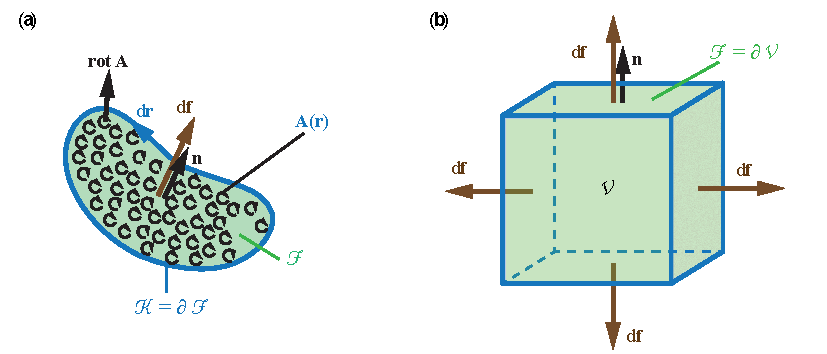
\includegraphics[width=\textwidth]{IntegralsaetzeEdyn.pdf}
  \caption[Orientierte Fl�chen f�r die Integrals�tze.]{Orientierte Fl�chen f�r die Integrals�tze. a) Stokes-Integralsatz. Das Oberfl�chenelement $d\vec{f}$ kann geschrieben werden als: $\D \vec{f} = \vec{n}\, \D f$, worin $ \vec{n}$ der Normalenvektor auf die Fl�che $\mathcal{F}$ ist. b) Gau�-Integralsatz. Auch hier ergibt sich das Oberfl�chenelement durch  $\D \vec{f} = \vec{n}\, \D f$. Wir bezeichnen hier den Volumenbereich mit $\mathcal{V}$, Fl�chen \bzw Oberfl�chen mit $\mathcal{F}$ und Konturen/Linien mit $\mathcal{K}$, das Symbol $\d$ bedeutet in diesem Kontext Berandung, $\d \mathcal{F}$ ist also die Berandung von $\mathcal{F}$ und somit eine Kontur $\mathcal{K}$.}
  \label{abb:kontmech_Integralsaetze}
\end{figure}


\subsubsection{Integralsatz von Stokes} \label{kap:kontmech_Integralsatz_Stokes}

Als erstes geben wir ohne Beweis (wir verweisen auf die Literatur \zb \cite{Otto2019, Fischer2018} und \cite{Schmutzer2005, Bartelmann2015}) den Integralsatz von Stokes an, der auch als Rotationssatz bekannt ist:
\begin{align}
    \int\displaylimits_{\mathcal{F}} \rotv \,\vec{A} \:\D\vec{f} &= \oint\displaylimits_{\mathcal{K} = \d \mathcal{F}} \vec{A}\cdot \D \vec{r} \quad~~\text{\bzw}\quad~~
    \int\displaylimits_{\mathcal{F}} \epsilon_{ijk}\,\d_{j} A_k \:\D f_{i} = \oint\displaylimits_{\mathcal{K} = \d \mathcal{F}} A_k \: \D x_{k} \,. \label{eq:kontmech_Integralsatz_Stokes}
\end{align}
Er besagt, dass ein Fl�chenintegral �ber die Rotation eines Vektorfeldes in ein geschlossenes Kurvenintegral �ber die Tangentialkomponente des Vektorfeldes umgewandelt werden kann. Dies ist hilfreich, da das Kurvenintegral das Vektorfeld allein enth�lt und keine Ableitung desselben und in der Regel einfacher zu berechnen ist als ein Fl�chenintegral.
Der Integralsatz von Stokes\index{Integralsatz von Stokes}\indexp{Stokes, Sir George Gabriel} findet in der Elektrodynamik breite Anwendung.

\subsubsection{Integralsatz von Gau�} \label{kap:kontmech_Integralsatz_Gauss}

Der Integralsatz von Gau�\index{Integralsatz von Gau�}\indexp{Gau�, Johann Carl Friedrich} l�sst sich �ber den Integralsatz von Stokes herleiten. Auch hier verweisen wir auf die Literatur \zb \cite{Otto2019, Fischer2018, Schmutzer2005, Bartelmann2015}: \\

\begin{align}
    \int\displaylimits_{\mathcal{V}} \divv\,\vec{A}\:\D V\,&= \oint\displaylimits_{\mathcal{F} = \d \mathcal{V}} \vec{A}\cdot \D \vec{f}\, \quad~~\text{\bzw}\quad~~
    \int\displaylimits_{\mathcal{V}} \d_{i}\,A_i \:\D V\,= \oint\displaylimits_{\mathcal{F} = \d \mathcal{V}} \,A_i\:\D f_{i} \,.  \label{eq:kontmech_Integralsatz_Gauss}
\end{align}

Mit den Integrals�tzen kann man, ohne weiter auf spezielle Koordinaten zur�ckgreifen zu m�ssen, anschaulich erkl�ren, warum Gradientenfelder wirbelfrei und Wirbelfelder quellenfrei sind. In \probref{kontmech_integralsaetze} berechnen wir die Integrale \eqref{eq:kontmech_Integralsatz_Stokes} und \eqref{eq:kontmech_Integralsatz_Gauss} 
f�r verschiedene Vektorfelder jeweils nach beiden Seiten der Gleichungen.

\subsubsection{Zerlegungssatz f�r Vektorfelder} \label{kap:kontmech_Zerlegungssatz}\index{Zerlegungssatz!Vektorfelder}

Der Zerlegungssatz f�r Vektorfelder lautet: Jedes �berall stetige und im Unendlichen verschwindende Vektorfeld $\vec{A}$ l�sst sich eindeutig als Summe eines wirbelfreien und eines quellenfreien Feldes darstellen:
\begin{align*}
    \vec{A} = \vec{A}^{\lk q\rk}+ \vec{A}^{\lk w\rk} \,,
\end{align*}
worin $\vec{A}^{\lk q\rk}$ das Quellenfeld und $\vec{A}^{\lk w\rk}$ das Wirbelfeld bezeichnen.
Die beiden Feldanteile lassen sich beschreiben durch:\
\begin{align}
    \vec{A}^{\lk q\rk}(\vec{r})&= -\gradv  \lk \frac{1}{4\pi}\int\limits_\mathcal{V} \frac{\divv \vec{A}\lk \vec{r}'\rk}{|\vec{r} - \vec{r}'|}\,\D V'\rk \label{eq:wirbelfeld01} \,, \\
    \vec{A}^{\lk w\rk}(\vec{r})&= +\rotv \lk \frac{1}{4\pi}\int\limits_{\mathcal{F} = \d \mathcal{V}} \frac{\rotv \vec{A}\lk \vec{r}'\rk}{|\vec{r} - \vec{r}'|}\,\D f'\rk \label{eq:wirbelfeld02}
\end{align}
Wir verweisen auf \cite{Schmutzer2005}, wo f�r diese Darstellungen von $\vec{A}^{\lk q\rk}$ \bzw  $\vec{A}^{\lk w\rk}$ nach einer etwas l�ngeren Rechnung folgende Beziehungen bewiesen werden k�nnen:
\begin{align}
    \rotv \vec{A}^{\lk q\rk} = 0\,,\,\divv  \vec{A}^{\lk q\rk} = \divv \vec{A} ~~~~\text{und} ~~~ \divv \vec{A}^{\lk w\rk} = 0 \,,\,\rotv \vec{A}^{\lk w\rk} = \rotv \vec{A}\,. \label{eq:wirbelfeld03}
\end{align}
%Das bedeutet, dass au�er Quellen und Wirbel keine weitere Ursachen f�r eine Wirbelbildung in Frage kommen. \\

Mit diesem Handwerkszeug der Vektoranalysis sind wir nun gut ger�stet, um die Beschreibung der Bewegungsvorg�nge in kontinuierlichen K�rpern in Angriff zu nehmen. 
%\textbf{Green'sche Integrals�tze:
%\begin{align}
    %\int\displaylimits_{\text{V}}\D V \lek\lk\vec{\nabla} \phi \rk\lk \nablav \chi\rk + \phi\,\Delta\chi\rek &=  \oint\displaylimits_{\d V}\D \vec{A}\,\phi\,\vec{\nabla}\chi ~~~\text{\bzw}\\
    %\int\displaylimits_{\text{V}}\D V\,\lk\phi\,\Delta\chi-\chi\,\Delta\phi\rk &= \oint\displaylimits_{\d V} \D \vec{A}\,\lk\phi\,\vec{\nabla}a\chi-\chi\,\vec{\nabla}\phi\rk\,.
%\end{align}

\clearpage
\section{Kinematik und Dynamik kontinuierlicher K�rper}
\label{kap:kontmech_kindyn}

\subsection{Materiepunkte und Koordinaten}
\label{kap:kontmech_materiepunkte} \index{Koordinaten!kontinuierliche K�rper}

Um Bewegungen kontinuierlicher K�rper beschreiben zu k�nnen, ben�tigen wir
zun�chst Koordinaten, in denen wir sie beschreiben k�nnen. Anders als beim
starren K�rper ist es nun bei Fluiden nicht mehr sinnvoll, ein unver�nderliches
k�rperfestes Koordinatensystem einzuf�hren, da sich der K�rper (das Fluid) selbst
mit der Zeit �ndern kann und sich einzelne Teile des Fluids gegeneinander
bewegen k�nnen. Sie w�ren also auch in einem k�rperfesten System nicht mehr
unver�nderlich. Zur Beschreibung greift man einzelne Materiepunkte wie den
Punkt~$\vec{\hat{P}}$ in \figref{kontmech_KontKoerpKoord01} heraus und
betrachtet das infinitesimale Volumen $V$ um diese herum.

\begin{figure}
  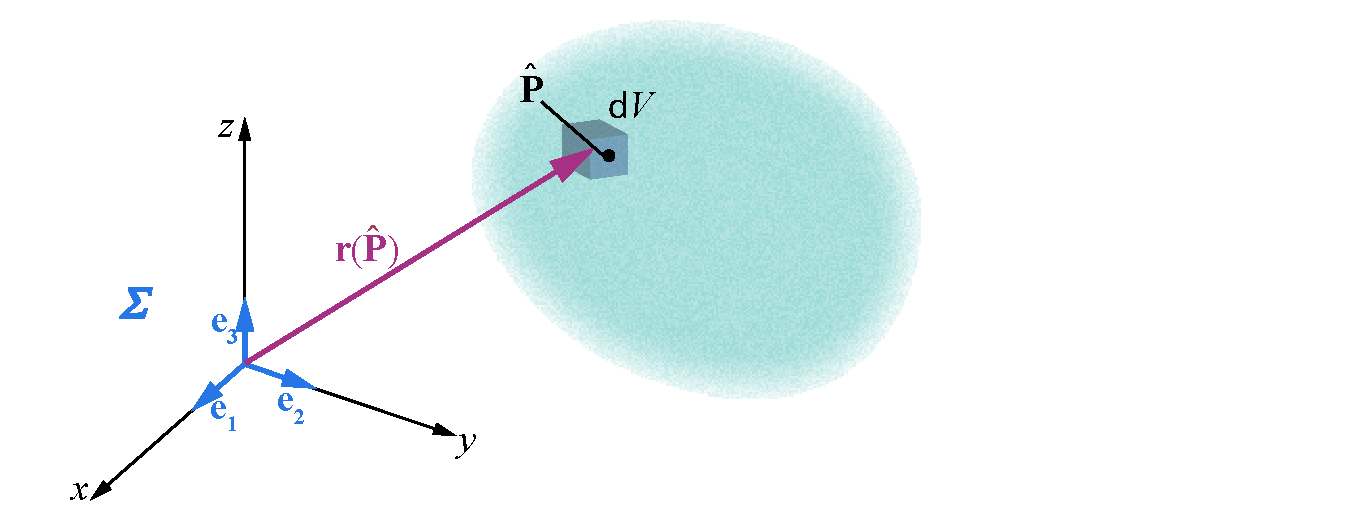
\includegraphics[width=\textwidth]{KontKoerpKoord.pdf}
  \caption[Materiepunkt und Raumpunkt eines kontinuierliechen K�rpers]{In der
    Beschreibung eines kontinuierlichen K�rpers ordnet man jedem Materiepunkt
    $\hat{\vec{P}}$ des K�rpers einen Raumpunkt $\vec{r}$ zu.}
    \label{abb:kontmech_KontKoerpKoord01}
\end{figure}

Der K�rper ist dann durch die Ansammlung eines Kontinuums von Materiepunkten
$\vec{\hat{P}}$ und die darin enthaltene Masse $\D m(\vec{\hat{P}})
= \varrho(\vec{\hat{P}})\,\mathrm{d}V$ beschrieben. Die Beschreibung erfolge in
einem raumfesten Koordinatensystem \vec{\Sigma}. Die zugeh�rigen Vektoren
nennen wir, wie wir es aus den vorherigen Kapiteln gewohnt sind, $\vec{r}
= \sum x_i\, \vec{e}_i\,, i=1 \ldots 3 $. Die Punkte $\vec{\hat{P}}$ kann man
dadurch festlegen, dass man ihnen Koordinaten in $\vec{\Sigma}$ zu einem festen
Zeitpunkt $t_0$ zuordnet,
\begin{equation}
  \vec{\hat{P}} \Leftrightarrow \vec{r}(\vec{\hat{P}},t_0) \; .
  \label{eq:kontmech_Materiepunkt}
\end{equation}

Damit bieten sich zwei M�glichkeiten, den
kontinuierlichen K�rper zu beschreiben. Wir k�nnen einerseits angeben,
an welchen Orten $\vec{r}$ sich die Materiepunkte $\vec{\hat{P}}$ in $\vec{\Sigma}$ 
befinden\footnote{Wir bezeichnen somit die Koordinaten eines Punktes
  $\vec{\hat{P}}$ mit dem Vektor $\vec{r}(\vec{\hat{P}})$. $\vec{\hat{P}}$ ist
  nicht zu verwechseln mit dem sp�ter eingef�hrten Druck $p$ im Fluid.}
\begin{subequations}
  \begin{equation}
    \vec{r} = \vec{r}(\vec{\hat{P}},t) \,.
    \label{eq:kontmech_EulerKoord}
  \end{equation}
  Dies nennt man in der Kontinuumsmechanik \gls{eulerscheKoordinaten}\index{Euler-Koordinaten}\indexp{Euler, Leonhard}. Bei der Eulerschen Beschreibung bleibt das \KOS quasi ortsfest. Wenn man eine physikalische Gr��e wie \zb die Geschwindigkeit $\vec{v}$ an einem Ort $\vec{r}$ zur Zeit $t$ betrachtet, so beschreibt diese Gr��e zu verschiedenen Zeiten verschiedene Fluidelemente $\vec{\hat{P}}_i$.\\
	Andererseits kann man einen kontinuierlichen K�rper auch dadurch beschreiben, dass
  man angibt, welcher materielle Punkt $\vec{\hat{P}}$ sich zu einer Zeit $t$
  am Ort $\vec{r}$ befindet,
  \begin{equation}
    \vec{\hat{P}} = \vec{\hat{P}}(\vec{r},t) \; .
    \label{eq:kontmech_LagrangeKoord}
  \end{equation}
  Dies sind \gls{lagrangescheKoordinaten}\index{Lagrange-Koordinaten}\indexp{Lagrange, Joseph-Louis}. Diese werden dadurch erm�glicht,
  dass niemals zwei materielle Punkte sich am selben Ort befinden k�nnen.
  Dadurch wird Gleichung \eqref{eq:kontmech_EulerKoord} umkehrbar und
  \eqref{eq:kontmech_LagrangeKoord} kann immer angegeben werden. Bei einer Beschreibung nach Lagrange wird das \KOS quasi mit den Materiepunkten mitbewegt, in der Beziehung \eqref{eq:kontmech_LagrangeKoord} beziehen wir uns immer auf das gleiche Fluidelement $\hat{\vec{P}}$.
\end{subequations}

\subsection{Kinematik}
\label{kap:kontmech_kinematik} \index{Kinematik!kontinuierliche K�rper}

\subsubsection{Geschwindigkeiten und Str�mungen}
\label{kap:kontmech_Geschwindigkeit} \index{Geschwindigkeit!kontinuierliche K�rper} \index{Str�mung}

Wir wollen nun im Sinne der Newtonschen Mechanik die Bewegung der Materiepunkte des Fluids betrachten. Die Geschwindigkeit eines Materiepunktes ist, da dieser nach
\eqref{eq:kontmech_Materiepunkt} selbst in der Zeit unver�nderlich ist, nur
von der �nderung seiner Position abh�ngig,
\begin{subequations}
  \begin{equation}
    \vec{v}(\vec{\hat{P}} ,t) = \frac{\D}{\D t} \vec{r}(\hat{\vec{P}},t) = \frac{\partial}
    {\partial t}\vec{r}(\vec{\hat{P}} ,t) \; . \label{eq:kontmech_GeschwZeit}
  \end{equation}
  Dies stellt die Geschwindigkeit dar, die ein Materiepunkt zum Zeitpunkt $t$
  hat. Dieser Materiepunkt �ndert dabei nat�rlich seinen Ort mit der Zeit.
  M�chte man die Geschwindigkeit wissen, die ein beliebiger Materiepunkt zum
  Zeitpunkt $t$ an einem bestimmten Ort $\vec{r}$ hat, muss man die
  Lagrangekoordinate \eqref{eq:kontmech_LagrangeKoord} in die Beziehung \eqref{eq:kontmech_GeschwZeit} f�r die Geschwindigkeit
  einsetzen und man erh�lt
  \begin{equation}
    \vec{v}(\vec{r},t) = \vec{v}(\vec{\hat{P}}(\vec{r},t),t) \; .
    \label{eq:kontmech_GeschwOrt}
  \end{equation}
\end{subequations}

Bei dieser Betrachtung wird gleich deutlich, dass man mit einer Geschwindigkeit
in einer Fl�ssigkeit oder einem Gas verschiedene physikalische Sichtweisen
meinen kann. Die gesamte Bewegung des Fluids zu einem Zeitpunkt $t$ nennt man \textit{Str�mung}\index{Str�mung}. Diese Str�mung l�sst sich
entsprechend auch auf verschiedene Arten beschreiben. Ein Spezialfall ist eine
\emph{station�re Str�mung}, die in der Zeit konstant ist, f�r die also gilt 
$\vec{v}(\vec{r},t) = \vec{v}(\vec{r})$.

Die Ortskurve, die ein bestimmter Materiepunkt in der Zeit durchl�uft, nennt
man eine \gls{Bahnlinie}\index{Bahnlinie}. Ist das Geschwindigkeitsfeld
\eqref{eq:kontmech_GeschwOrt} bekannt, erh�lt man die Bahnlinie durch
Integration von diesem Geschwindigkeitsfeld $\vec{v}(\vec{r},t)$ �ber die Zeit.

Die Linie, die immer tangential an das Geschwindigkeitsfeld zu einem festen
Zeitpunkt~$t$ anliegt, nennt man eine \gls{Stromlinie}\index{Stromlinie}.
Diese Stromlinien stellen dar, wie die Str�mung zum aktuellen Zeitpunkt $t$ 
verl�uft. In jedem Raumpunkt befindet sich dabei ein anderer Materiepunkt und
hat aktuell diese Geschwindigkeit $\vec{v}(\vec{r},t)$. Dies muss nicht mit der Bahnkurve
�bereinstimmen, siehe \figref{kontmech_KontKoerpKoord02}. In einer station�ren
Str�mung werden jedoch beide Linien �bereinstimmen.

\begin{figure}
  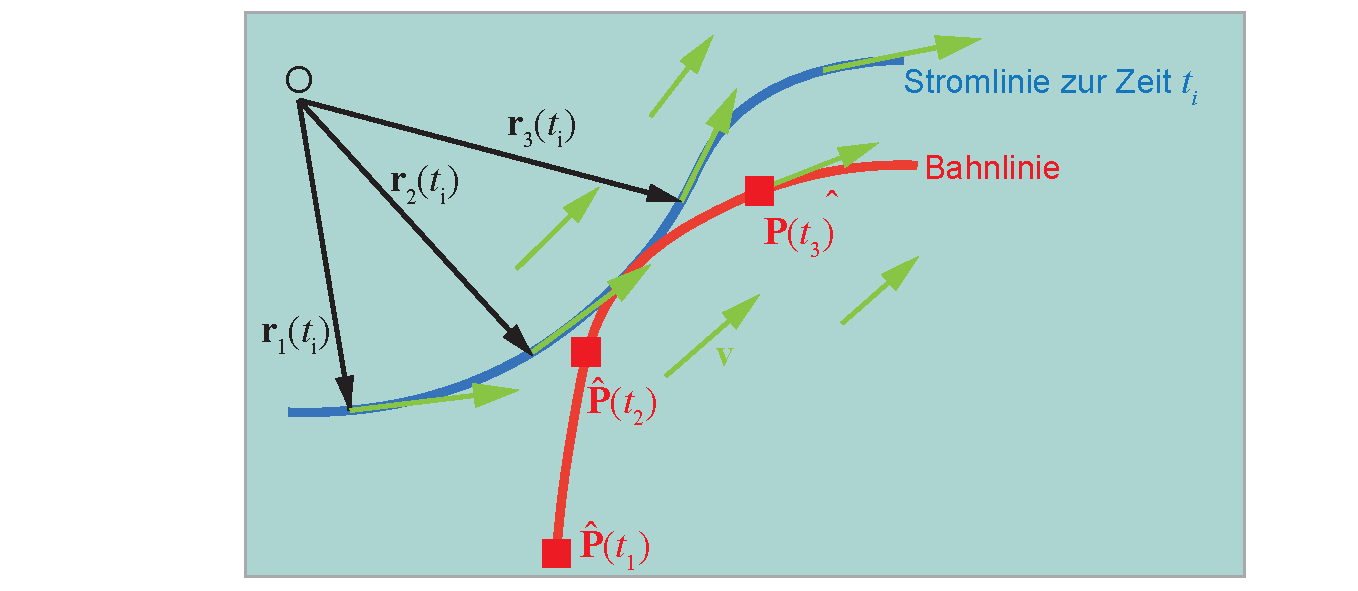
\includegraphics[width=\textwidth]{KontStromlinie.pdf}
  \caption[Bahn- und Stromlinie einer Str�mung]{Eine \gls{Stromlinie} (blau)
    liegt tangential am Geschwindigkeitsfeld zu einem festen Zeitpunkt (gr�ne
    Pfeile) an. Im Gegensatz dazu beschreibt eine \gls{Bahnlinie} (rot) die
    Ortskurve, die ein Materiepunkt mit der Zeit durchl�uft.}
    \label{abb:kontmech_KontKoerpKoord02}
\end{figure}

Str�mungen werden sehr stark von inneren Reibungen beeinflusst. Das trifft
besonders stark auf Fl�ssigkeiten zu. Weil die Reibung, die wir mit der sp�ter 
zu definierenden Viskosit�t\index{Viskosit�t} bezeichnen wollen (siehe \kap{kontmech_InnereReibung}),  dabei das Verhalten
der str�menden Fl�ssigkeit in der Art der Str�mung sehr stark beeinflussen
kann, unterscheidet man je nach St�rke der Reibung die Art der Str�mung.
Eine \emph{ideale Fl�ssigkeit}\index{Fl�ssigkeit!ideale} wird dabei kaum von
der Reibung beeinflusst.
Sie ist dadurch gekennzeichnet, dass die Reibungskr�fte klein gegen alle
anderen an der Fl�ssigkeit angreifenden Kr�fte sind. Dieses Verhalten trifft
meist auch auf Gase zu.  Im Gegensatz dazu ist eine \emph{stark viskose
  Fl�ssigkeit} eine, in der die Reibungskr�fte dominieren. Die meisten
\emph{realen Fl�ssigkeiten} befinden sich im Bereich dazwischen.

Eine Str�mung wird als \emph{laminar}\index{Str�mung!laminar} bezeichnet,
wenn \gls{Bahnlinie}n benachbarter
Materiepunkte nebeneinander liegen, ohne sich zu durchmischen. Viskose
Fl�ssigkeiten tendieren zu einem laminaren Str�mungsverhalten, weil hier die
Reibungskr�fte gegen�ber den beschleunigenden Kr�ften dominieren. Ist die
Reibung klein gegen die beschleunigenden Kr�fte, kann das Str�mungsbild unruhig
werden. Das geschieht insbesondere dann, wenn die Fl�ssigkeit an ihren
Grenzen (\zb dem Rand eines Rohres) durch st�rkere Reibungskr�fte an diesem
Rand beeinflusst wird. In diesem Fall kann die Str�mung
\emph{turbulent}\index{Str�mung!turbulent} werden (siehe auch �bersicht \ref{tab:kontmech_stroemung_overview}).


\subsubsection{Beschleunigungen}
\label{kap:kontmech_Beschleunigung} \index{Beschleunigung!kontinuierliche K�rper}

Als \emph{materielle}\index{Beschleunigung!materielle} oder
\emph{substantielle Beschleunigung}\index{Beschleunigung!substantielle}
definieren wir die Beschleunigung, die ein Materieteilchen am Ort $\vec{r}$
erf�hrt,\dh in dem wir \eqref{eq:kontmech_GeschwOrt} ableiten:
\begin{align}
\begin{split}
  \vec{a}(\vec{r},t) &= \frac{\D}{\D t} \vec{v}(\vec{r},t) = \dot{\vec{v}}(\vec{r},t)
  = \sum_{i=1}^3 \frac{\partial \vec{v}(r,t)}{\partial x_i} \frac{\D x_i}{\D t} \,\vec{e}_i
  + \frac{\partial}{\partial t} \vec{v}(\vec{r},t) \\
  &= \lk \vec{v}(\vec{r},t) \cdot \nablav \rk \vec{v}(\vec{r},t)
  + \frac{\partial}{\partial t} \vec{v}(\vec{r},t) \; . 
\end{split} \label{eq:kontmech_Beschleunigung}
\end{align}
Man erkennt hier die Dyade $\cdot \nablav$ \eqref{eq:kontmech_nablaop03} wieder und dass es zwei Beitr�ge zur �nderung der Geschwindigkeit gibt.
Einerseits kann sich das Geschwindigkeitsfeld mit der Zeit selbst �ndern.
Dies wird durch die partielle Ableitung im zweiten Term beschrieben. Der
erste Term ber�cksichtigt, dass sich der Materiepunkt an einen anderen
Raumpunkt bewegt und somit auch der r�umlichen �nderung des
Geschwindigkeitsfeldes unterliegt. Diesen Teil der Beschleunigung nennt man
\emph{Konvektionsbeschleunigung}\index{Konvektionsbeschleunigung}\index{Beschleunigung!Konvektions-}. 
Man erkennt an \eqref{eq:kontmech_Beschleunigung} wieder, 
dass wir bei der Beschreibung von Kinematik und Dynamik des Kontinuums auf partielle Differentialgleichungen 
treffen.

\subsection{Eigenschaften von Str�mungen}
\label{kap:kontmech_EigenschaftenStroemungen} 
\subsubsection{Stromdichte, Fluss und Kontinuit�tsgleichung}
\label{kap:kontmech_Stromdichte}\index{Kontinuit�tsgleichung!kontinuierliche K�rper}

Bei der Betrachtung von Str�mungen interessiert man sich oft daf�r, wie
sich die Materie, die eine Dichte $\varrho$ haben soll, bewegt. Dazu f�hren wir die \emph{Stromdichte}\index{Stromdichte}
\begin{equation}
  \vec{j} = \varrho \,\vec{v}
  \label{eq:kontmech_Stromdichte}
\end{equation}
ein, die nicht nur die Geschwindigkeit beschreibt, sondern beschreibt, wie
sich die Materie mit dieser Geschwindigkeit bewegt. In einem differentiellen
Volumenelement erhalten wir
\begin{equation*}
  \vec{j}\,\D V = \varrho\,\D V\,\vec{v} = \D m \, \vec{v} \; .
\end{equation*}
Die Stromdichte tritt also f�r das kontinuierliche System an die Stelle
des Impulses und hat die Einheit einer Impulsdichte ($\SI{}{\kg\per\metre\squared\per\second}$).

Der \emph{Fluss}\index{Fluss} einer Str�mung durch eine Oberfl�che l�sst sich durch
\begin{equation*}
  \Phi = \int_A \vec{j} \cdot \D\vec{A} = \int_A \varrho \,\vec{v} \cdot
  \D\vec{A}
\end{equation*}
berechnen und gibt an, wie viel der Materie in einer gewissen Zeit durch
die Querschnittsfl�che $A$ flie�t.

Der Fluss ist ebenfalls entscheidend, wenn wir die Masse in einem
bestimmten, zeitlich konstanten Volumenelement betrachten m�chten. Diese
k�nnen wir jederzeit durch das Integral
\begin{equation*}
  m = \int_V \varrho\,\D V
\end{equation*}
berechnen. Die Massenerhaltung verlangt, dass die zeitliche �nderung
der Masse im Volumen gerade der Masse entspricht, die zu- bzw. abflie�t.
Man kann also die Erhaltungsgleichung
\begin{equation*}
  \frac{\partial}{\partial t} M = \int_V \frac{\partial}{\partial t}\varrho\,\D V 
  = -\int_{A = \partial V} \vec{j}\cdot \D\vec{A} = \Phi 
\end{equation*}
aufstellen, wobei das Oberfl�chenintegral gerade �ber den gesamten Rand
des Volumens~$V$ geht, den wir mit $\partial V$ bezeichnen wollen, $\Phi$ ist der Materiefluss in $\SI{}{\kg\per\second}$. Das Minus\-zeichen r�hrt daher, dass die Randfl�che
nach au�en orientiert ist. Das Skalarprodukt $\vec{j}\cdot \D\vec{A}$
liefert also dann einen positiven Wert, wenn es einen Netto-Abfluss von
Masse gibt. Mit dem Integralsatz von Gau� \eqref{eq:kontmech_Integralsatz_Gauss} l�sst sich das Oberfl�chenintegral
umformen, so dass wir 
\begin{equation}
  \int_V \frac{\partial}{\partial t}\varrho\,\D V 
  = -\int_V \divv \vec{j}\, \D V
  \label{eq:kontmech_KontinuitaetsglMakr}
\end{equation}
erhalten.

Gleichung \eqref{eq:kontmech_KontinuitaetsglMakr} muss f�r jedes beliebige
Volumen gelten. Wir haben nur vorausgesetzt, dass dieses zeitlich konstant sein
soll. Damit l�sst sich dann die differentielle Form der
\emph{Kontinuit�tsgleichung}\index{Kontinuit�tsgleichung}
\begin{equation}
  \frac{\partial}{\partial t}\varrho + \divv \vec{j} =
  \frac{\partial}{\partial t}\varrho + \divv \lk \varrho\, \vec{v} \rk = 0
  \label{eq:kontmech_KontinuitaetsglDiff}
\end{equation}
aufstellen.

Ein interessanter Spezialfall sind \emph{inkompressible} Fl�ssigkeiten\index{Fl�ssigkeit!inkompressible}.
Diese zeichnen sich dadurch aus, dass ihre Dichte zeitlich und r�umlich
konstant ist. Das hei�t $\partial \varrho/ \partial t = 0$ und $\divv\lk
\varrho\, \vec{u} \rk = \varrho \divv \vec{u}$. Im Fall imkompressibler Fluide vereinfacht sich
die Kontinuit�tsgleichung zu
\begin{equation}
  \divv \vec{v}  = 0 \; .
  \label{eq:kontmech_KontinuitaetsglInkompr}
\end{equation}
Das Str�mungsfeld weist also keine Divergenzterme auf. Dies entspricht der
Tatsache, dass an keinem Punkt in der inkompressiblen Fl�ssigkeit Masse
konzentriert oder ausged�nnt werden kann. 

\subsubsection{Formen von Str�mungen}
\label{kap:kontmech_FormenStroemungen}\index{Str�mung!Formen}

Str�mungen k�nnen sehr unterschiedliche Formen annehmen. Wir wollen vor
allem laminare und turbulente Str�mungen unterscheiden.

\index{Str�mung!laminar|textbf}%
Als \emph{laminar} bezeichnen wir Str�mungen, bei denen verschiedene
Schichten der Fl�ssigkeit oder des Gases sich nicht miteinander mischen. Das hei�t
nicht, dass sie sich alle identisch bewegen m�ssen. Sie k�nnen \zb
unterschiedliche Geschwindigkeiten haben, gleiten dann aber glatt aneinander
vorbei. Beispiele sind in \figref{kontmech_FormenStroemungen}a gezeigt.
Laminare Str�mungen treten immer dann auf, wenn der Energie�bertrag innerhalb
der Fl�ssigkeit oder des Gases gro� ist, also die interne Reibung eine gro�e
Rolle spielt und damit die Bewegung des Kontinuums dominiert. 

\begin{figure}
  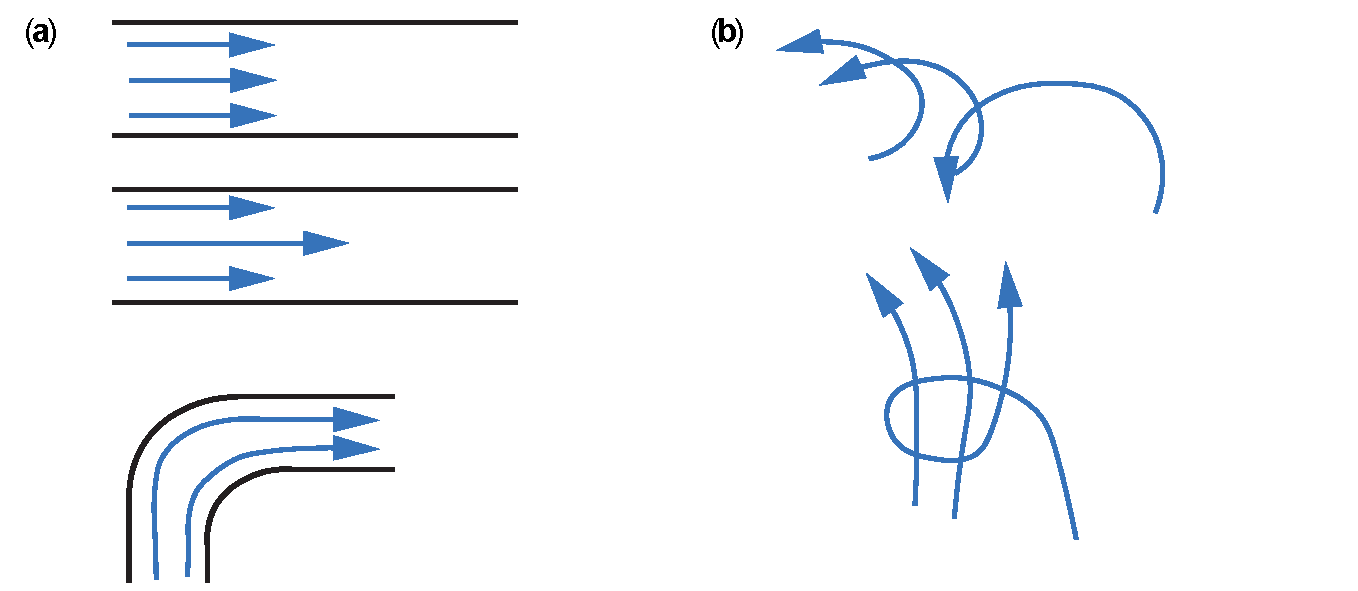
\includegraphics[width=\textwidth]{FormenStroemungen.pdf}
  \caption[Formen von Str�mungen]{Formen von Str�mungen. \fa In laminaren
    Str�mungen gleiten unterschiedliche Schichten glatt, \dh ohne Vermischung, aneinander vorbei.
    \fb In turbulenten Str�mungen schneiden sich die \gls{Bahnlinie}n der
    einzelnen Schichten. Es kommt zu Durchmischungen der Schichten.}
  \label{abb:kontmech_FormenStroemungen}
\end{figure}

\index{Str�mung!turbulent|textbf}%
Sobald dies nicht mehr erf�llt ist, k�nnen die verschiedenen Schichten leicht
ineinander eindringen, verwirbeln  und miteinander mischen. Solche Str�mungen
nennen wir \emph{turbulent}. Beispiele daf�r sind in
\figref{kontmech_FormenStroemungen}b gegeben.
  
Ein weiteres wesentliches Charakteristikum von Str�mungen ist ihre \emph{Rotation}\index{Str�mung!Rotation}\index{Rotation!Str�mung}.
Rechnerisch ergibt sich diese aus der Geschwindigkeit durch $\rotv \vec{v}$.
Sie gibt an, ob sich Objekte, die sich in der Str�mung bewegen, in
eine Rotationsbewegung versetzen lassen. Das ist sehr offensichtlich
bei vorhandenen Wirbeln der Fall. Tats�chlich sind aber auch rein gerade
Str�mungen nicht rotationsfrei. Im Beispiel nach \figref{kontmech_Rotation} sieht man, 
dass sich in einer gerade verlaufenden Str�mung mit in einer Dimension unterschiedlichen
Geschwindigkeiten ein Objekt drehen wird. Der zun�chst mit seiner langen Seite
senkrecht zur Str�mung ausgerichtete Balken wird an seinen beiden Enden
unterschiedlich schnell bewegt. F�r gr��ere Zeiten sieht man, wie sich das zu
einer Rotation ausbildet, die mit der Translationsbewegung des
Massenmittelpunkts in Str�mungsrichtung �berlagert ist.

\begin{figure}
  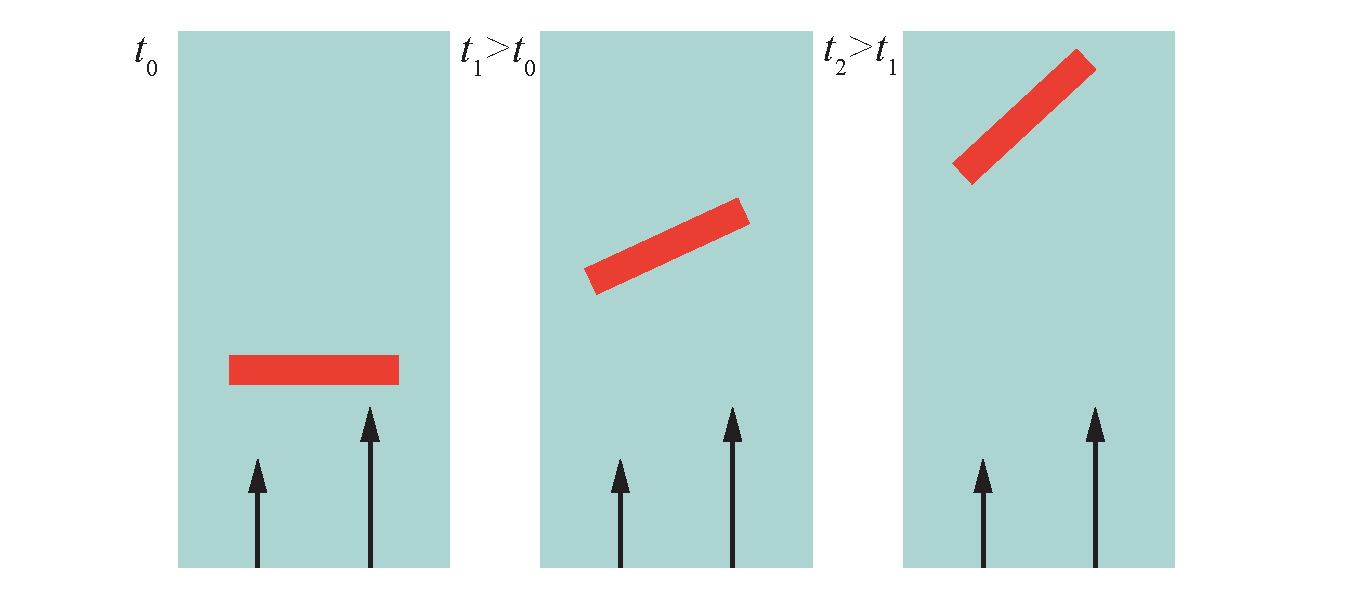
\includegraphics[width=\textwidth]{StroemungRotation.pdf}
  \caption[Nichtverschwindende Rotation in einer gerade Str�mung]
  {Nichtverschwindende Rotation in einer gerade in $z$-Richtung verlaufenden Str�mung mit unterschiedlichen
    Geschwindigkeiten in den einzelnen Schichten entlang $x$-Richtung.}
  \label{abb:kontmech_Rotation}
\end{figure}

Ein besonderer Fall der Str�mung eines Fluids ist die \emph{Potentialstr�mung}\index{Potentialstr�mung}, bei der das Geschwindigkeitsfeld $\vec{v}(\vec{r})$ ein Potential besitzt. Ein solches Potential ist in einem homogenen Fluid vorhanden, wenn die Str�mung wirbelfrei und die inneren Reibungskr�fte vernachl�ssigbar klein sind. Potentialstr�mungen k�nnen sehr vorteilhaft mit mathematischen Methoden der Potentialtheorie behandelt werden, wir verweisen hierzu auf die weiterf�hrende Literatur \cite{Schmutzer2005, Altenbach2018, Rannacher2017}.

\subsection{Dynamik kontinuierlicher K�rper}\label{kap:kontmech_dynamik}
\index{Dynamik!kontinuierliche K�rper}

\subsubsection{Euler-Gleichung}\indexp{Euler, Leonhard}
\label{kap:kontmech_EulerGl}\index{Euler-Gleichung (Kontinuumsmechanik)|textbf}

Auf eine Fl�ssigkeit oder ein Gas k�nnen mehrere Formen von Kr�ften angreifen.
Diese verursachen, wie es in Erweiterung der Newtonschen Bewegungsgleichungen
\eqref{eq:bew_NewtonBGL} sein muss, eine Beschleunigung des Volumenelements
$\D V$ aus \figref{kontmech_KontKoerpKoord02}. F�r dieses differentielle
Volumenelement formulieren wir unter Benutzung von \eqref{eq:kontmech_Beschleunigung} die Newtonschen Bewegungsgleichungen in
der Form
\begin{equation}
  \varrho\, \D V\, \vec{a}(\vec{r},t) = \sum_i \vec{F}_i  \label{eq:kontmech_kraefte_an_dV}
\end{equation}
mit der Summe aller am Volumenelement $\D V$ angreifenden Kr�fte. Dabei werden wir
drei Formen von Kr�ften unterscheiden:

\begin{enumerate}
\item Auf das Fluid wirken externe 
  \emph{Volumenkr�fte}\index{Volumenkr�fte}, die
  an jedem Raumpunkt direkt angreifen (wie \zb die Schwerkraft). Diese Kr�fte wollen wir mit
  \begin{equation*}
    \vec{F}_\text{V} = \vec{f}_\text{V} \D V
  \end{equation*}
  bezeichnen, wobei $\vec{f}_V$ die Kraftdichte darstellt.
\item Die Volumenelemente �ben �ber ihre Grenzfl�chen eine Kraft auf die benachbarten Elemente aus. Diese Kr�fte definieren den Druck $p(\vec{r}')$ an der Stelle $\vec{r}'$ auf ein Volumenelement $\D V$. Ist
  dieser Druck nicht homogen, resultiert eine Kraft auf das Volumen, die sich durch
  das Oberfl�chenintegral
  \begin{equation*}
    \vec{F}_\text{D} = -\int_{\partial V} p(\vec{r}')\, \D \vec{A}'
  \end{equation*}
  �ber den Rand $\partial V$ von $\D V$ berechnen l�sst, wobei das
  Fl�chenelement nach au�en orientiert ist. Das differentielle Volumenelement
  wollen wir durch einen W�rfel der Kantenl�nge $\Delta l$ beschreiben. Der
  Materiepunkt, auf den die Kraft wirkt, liege in der Mitte des W�rfels.
\begin{figure}
  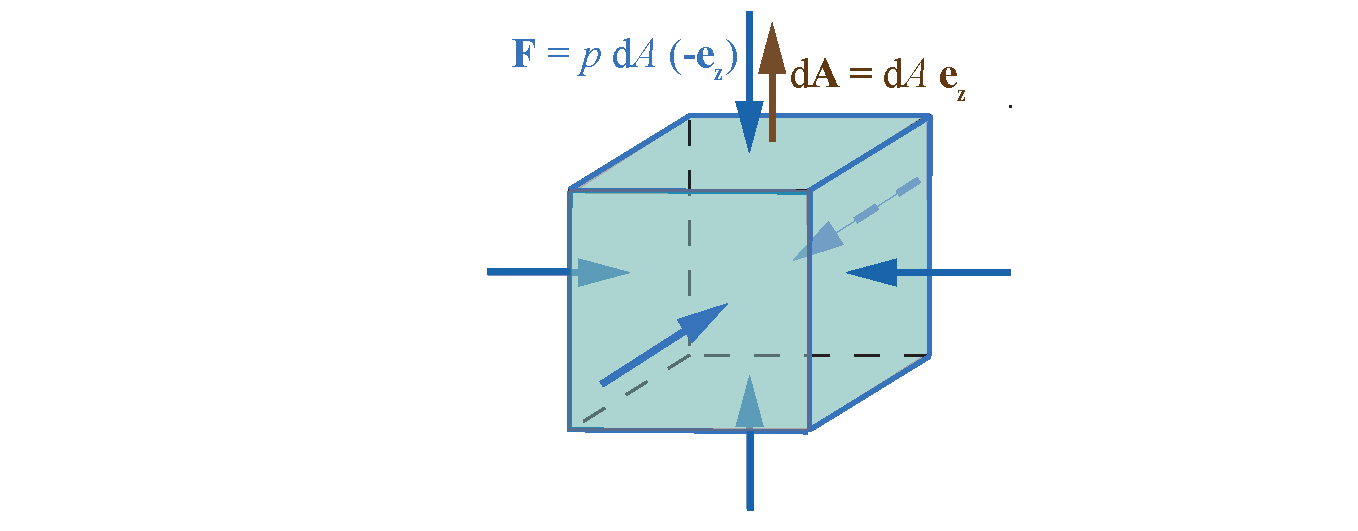
\includegraphics[width=\textwidth]{KontDruck.pdf}
  \caption[Druck auf das Volumenelement einer Fl�ssigkeit]{Druck auf das
    Volumenelement einer Fl�ssigkeit. Das Volumenelement wird durch einen
    W�rfel approximiert. Die Kr�fte wirken entgegen der nach au�en orientierten
    Normalenvektoren auf die Fl�che.}
  \label{abb:kontmech_KraefteDruck}
\end{figure}
  Dann wird das Integral (vgl. \figref{kontmech_KraefteDruck}) zu 
  \begin{align*}
    - \int_{\partial V} p(\vec{r}')\, \D \vec{A}'
    = &-p(x-\Delta l/2,y,z) \, \D A \, \lk -\veceX \rk - p(x+\Delta l/2,y,z)
        \, \D A \, \veceX \\
      &- p(x,y-\Delta l/2,z) \, \D A \, \lk -\veceY \rk  - p(x,y+\Delta l/2,z)
        \, \D A \, \veceY \\
      &- p(x,y,z-\Delta l/2) \, \D A \, \lk -\veceZ \rk  - p(x,y,z+\Delta l/2)
        \, \D A \, \veceZ \; .
  \end{align*}
  Ber�cksichtigen wir, dass im differentiellen Volumenelement eine
  Linearisierung des Drucks im Volumen ausreicht, so l�sst sich dies
  umschreiben zu
  \begin{equation*}
    \vec{F}_\text{D} = -\frac{\partial p(\vec{r})}{\partial x} \, \Delta l\, \D A \,\veceX 
		                   - \frac{\partial p(\vec{r})}{\partial y} \, \Delta l \, \D A \, \veceY 
											 - \frac{\partial p(\vec{r})}{\partial z} \, \Delta l \, \D A\, \veceZ \;  .
  \end{equation*}
Letztendlich erhalten wir also:
  \begin{equation}
    \vec{F}_\mathrm{D} = -\vec{\nabla} p\, \D V \;  .
    \label{eq:kontmech_Druckkraft}
  \end{equation}
	Wir haben hier bei der Ableitung vorausgesetzt, dass der
Druck jeweils senkrecht auf die Seitenfl�che des betrachteten differentiellen Volumenelements (W�rfel der Kantenl�nge $l$) wirkt.
Bei Fl�ssigkeiten ist das im Allgemeinen erf�llt, bei Festk�rperkontinua muss das nicht der Fall sein. Dann muss man den Gradienten des Drucks (einen Vektor) durch den sogenannten \textit{Spannungstensor} $\sigma$\index{Spannungstensor} ersetzen. Umgekehrt kann man sagen, dass f�r einen Spannungstensor, dessen Nichtdiagonalelemente alle 0 sind, die Diagonalelemente gerade den Gradienten des Drucks darstellen. Wir verweisen dazu auch \kap{kontmech_festelastisch}.
\item Es wirken Reibungskr�fte, die wir zun�chst ganz allgemein mit $\vec{F}_\text{R} = \vec{f}_\text{R}
  \D V$ bezeichnen wollen und sp�ter zwischen inneren Reibungen und Reibungen
  mit dem Rand unterscheiden werden. 
\end{enumerate}
In Summe erhalten wir also f�r \eqref{eq:kontmech_kraefte_an_dV} die
Bewegungsgleichung eines Materiepunkts in der Euler-Betrachtung im Kontinuum 
die \emph{Euler-Gleichung}\index{Euler-Gleichung (Kontinuumsmechanik)}
\begin{equation}
  \varrho \lk \lk \vec{v} \cdot \nabla \rk \vec{v} + \frac{\partial}{\partial t}
  \vec{v} \rk = \vec{f}_\text{V}  + \vec{f}_\text{R} - \vec{\nabla} p \; .
  \label{eq:kontmech_EulerGleichung}
\end{equation}

% BEISPIEL %%%%%%%%%%%%%%%%%%%%%%%%%%%%%%%%%%%%%%%%%%%%%%%%%%%%%%%%%%%%%%%%%%%%%%%%%%%%%%%%%%
\begin{example}{Wasserwellen}\index{Wasserwellen}
\label{bsp:kontmech_Wasserwellen}
Wir werden in \kap{kontmech_festLagrange} die Physik der Wellen, wie sie
in einem kontinuierlichen Medium entstehen, genauer untersuchen. Hier wollen
schon an einem ersten Beispiel zeigen, wie wir aus der Euler-Gleichung
\eqref{eq:kontmech_EulerGleichung} das Auftreten von Wasserwellen und deren
Wellenl�ngenabh�ngigkeit von der Wasserh�he absch�tzen k�nnen.\\
Wasserwellen sind Oberfl�chenwellen an der Grenzfl�che zwischen Wasser und Luft und haben Periodendauern von Sekunden bis mehrere Stunden (siehe Gezeitenwelle\index{Welle!Gezeiten-} \kap{bew_gezeiten}).
Wichtig f�r unsere Betrachtung ist, dass die Wasserteilchen nur relativ kleine Bewegungen ausf�hren, ihre Bewegungsenergie aber an benachbarte Teilchen weiter gibt.
Bei Wellenl�ngen kleiner als $\SI{1}{\centi\metre}$  bestimmen Oberfl�chenspannung und Z�higkeit des Wassers die Eigenschaften der Wellen, bei Wellenl�ngen gr��er als $\SI{10}{\centi\metre}$ ist die Erdanziehungskraft entscheiden, die Wasserwellen sind dann sogenannte Schwerewellen\index{Welle!Schwere-}.
Wasserwellen weichen in ihrer Gestalt von der �blichen Sinusform ab. Der Teil der Welle, der oberhalb des Ruhewasserspiegels ($z=0$) liegt, wird als Wellenberg bezeichnet, die h�chste Auslenkung als Wellenkamm. Der Teil unterhalb des Ruhewasserspiegels hei�t Wellental. Die Wellenh�he ist die Summe der Betr�ge der Maximalauslenkungen von Wellenberg und Wellental. Als Wellenl�nge $\lambda$ wird der Abstand zweier Wellenk�mme bezeichnet (\figref{kontmech_Wasserwellen}).

Wir wollen nun zeigen, wie wir aus der
Euler-Gleichung \eqref{eq:kontmech_EulerGleichung} mit der Gewichtskraft
als Volumenkraft,
\begin{equation}
  \vec{f}_\text{V} = - \varrho g \veceZ \; ,
\end{equation}
eine relevante Aussage f�r die Ausbreitung von Wasserwellen
in Abh�ngigkeit von der Wassertiefe erhalten k�nnen. Dazu arbeiten wir mit dem
Modell nach  \figref{kontmech_Wasserwellen} \cite{Mai2004}. Nach diesem Modell
bewegen sich  die Wassermolek�le nur in der $x$-$z$-Ebene und es k�nnen auch
nur in dieser Ebene  Druck�nderungen auftreten. Die $y$-Richtung wird als
unendlich ausgedehnt betrachtet.

Wir dr�cken die Materiepunkte (Wasserteilchen an der Oberfl�che)
$\vec{\hat{P}}$ f�r eine ruhende Wasseroberfl�che aus durch ihre
Ruhelage-Koordinaten $x_0$ und $z_0$aus. Ihre Lage in der bewegten Welle zum
Zeitpunkt $t$ ist dann durch
\begin{equation}
  x = x(x_0, z_0, t)\; , \quad z = z(x_0, z_0, t)
\end{equation}
gegeben. Die Oberfl�che des Wassers bezeichnen wir durch die Funktion
$Z_W(x,t)$ und es gilt
\begin{equation}
  z(x_0,z_0=0,t) = Z_\text{W}(x,t) \; ,
  \label{eq:kontmech_WasserwellenRBLuft}
\end{equation}
das hei�t die materiellen Punkte $\vec{\hat{P}}$ mit $z(0) = z_0 = 0$ befinden
sich immer auf dieser Oberfl�che $Z_\text{W}(x,t)$.

\begin{center}
  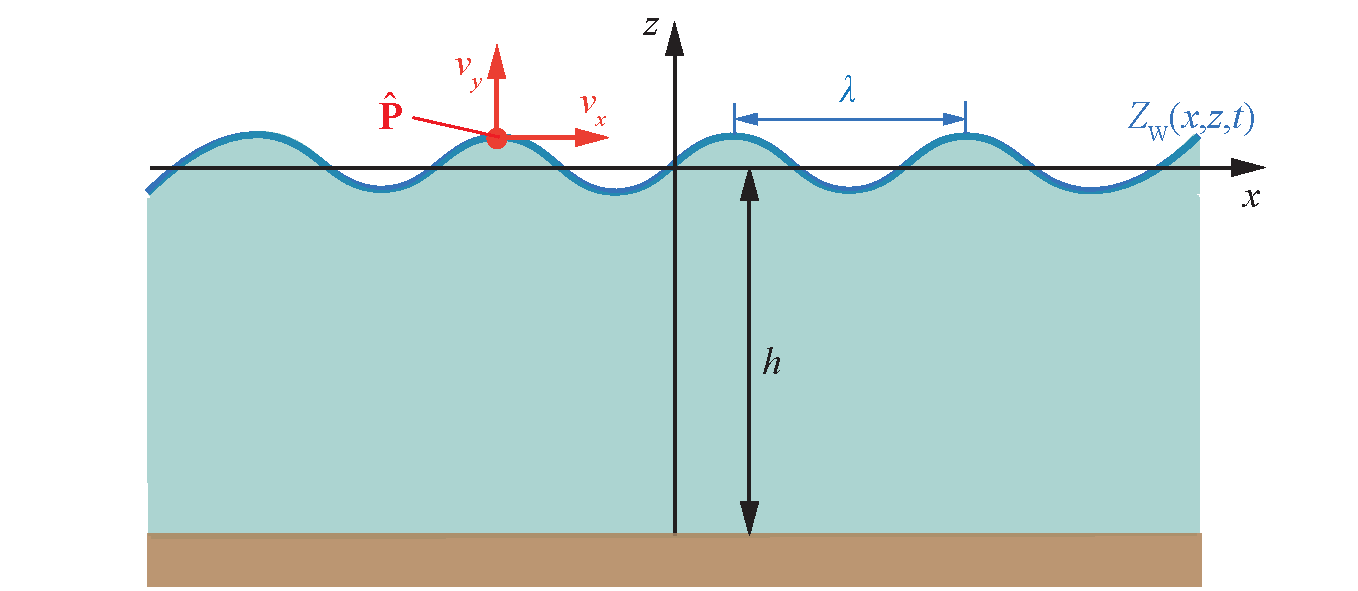
\includegraphics[width=\textwidth]{WasserwellenKoord.pdf}
  \captionof{figure}{Koordinatensystem f�r Wasserwellen.}%
  \label{abb:kontmech_Wasserwellen}
\end{center}

Zur L�sung des Problems m�ssen wir mehrere Gleichungen ber�cksichtigen. Als
erstes gehen wir von der Euler-Gleichung \eqref{eq:kontmech_EulerGleichung}
aus, in der wir entsprechend der Annahme �ber das Modell die
Geschwindigkeitskomponenten $v_x$ und $v_y$ ber�cksichtigen,
\begin{equation*}
  \vec{v} = \begin{pmatrix} v_x & 0 &v_z \end{pmatrix}^\text{T} \; .
\end{equation*}
Die Euler-Gleichung reduziert sich dann auf die Form
\begin{equation}
  \varrho \lk \lk v_x \frac{\partial}{\partial x} + v_z \frac{\partial}
  {\partial z} \rk \begin{pmatrix} v_x \\ 0 \\ v_z \end{pmatrix}
  + \frac{\partial}{\partial t} \begin{pmatrix} v_x \\ 0 \\ v_z \end{pmatrix}
  \rk =  - \begin{pmatrix} \partial p/\partial x \\ 0 \\
    \partial p/\partial z \end{pmatrix} + \varrho \begin{pmatrix} 0 \\ 0 \\ -g
  \end{pmatrix}\; .
  \label{eq:kontmech_WellenEulerGleichung}
\end{equation}

Da wir davon ausgehen, dass die Bewegung rotationsfrei zustande kommt
und eine reibungsfreie Fl�ssigkeit dann auch rotationsfrei bleibt (was in
\kap{kontmech_laminareStroemungenFluessigkeiten} genauer untersucht wird),
k�nnen wir das Geschwindigkeitsfeld auf eine skalare Funktion $\Psi(x,z,t)$
zur�ckf�hren,
\begin{equation}  \vec{v} = \nabla \Psi \; , \qquad v_x = \frac{\partial \Psi}
  {\partial x} \; , \quad v_z = \frac{\partial \Psi}{\partial z} \; .
  \label{eq:kontmech_WasserwellenPsi}
\end{equation}
Wir haben es also mit einer sogenannten \emph{Potentialstr�mung}\index{Str�mung!Potential-} zu tun. Ausgedr�ckt durch die skalare Funktion $\Psi(x,z,t)$ l�sst sich die vektorielle
Gleichung \eqref{eq:kontmech_WellenEulerGleichung} auf die skalare Darstellung
\begin{equation}
  \frac{\varrho}{2} \lk \frac{\partial \Psi}{\partial x} \rk^2
  + \frac{\varrho}{2} \lk \frac{\partial \Psi}{\partial z}  \rk^2
  + \varrho \frac{\partial \Psi}{\partial t} = - \varrho g z  - p + C
  \label{eq:kontmech_WellenEulerSkalar}
\end{equation}
mit einer beliebigen Konstanten $C$ zur�ckf�hren. Davon kann man sich leicht
�berzeugen, wenn man den Gradienten von Gleichung
\eqref{eq:kontmech_WellenEulerSkalar} bildet und dabei mit
\eqref{eq:kontmech_WasserwellenPsi} ber�cksichtigt, dass
$\Psi$ und $p$ nicht von der Koordinate $y$ abh�ngen.

Die Gleichung \eqref{eq:kontmech_WellenEulerSkalar} kann nun
herangezogen werden, den Druck im Wasser zu bestimmen. Eine wertvolle Information
f�r die Wellenausbreitung erhalten wir, indem wir ber�cksichtigen, dass
Gleichung \eqref{eq:kontmech_WellenEulerSkalar} insbesondere auch an der
Grenzschicht zwischen der Wasseroberfl�che und der Luft gelten muss. Hier
kennen wir den Druck und wissen, dass er (bis auf vernachl�ssigbar kleine
�nderungen mit $Z_W(x,t)$) konstant dem Atmosph�rendruck $p_\mathrm{atm}$
entsprechen muss. Da die Gleichung f�r jede beliebige Konstante $C$ gilt,
w�hlen wir zur Vereinfachung $C = -p_\mathrm{atm}$ und erhalten
\begin{equation}
  \frac{\varrho}{2} \lk \frac{\partial \Psi(x,z=0)}{\partial x} \rk^2
  + \frac{\varrho}{2} \lk \frac{\partial \Psi(x,z=0)}{\partial z}  \rk^2
  + \varrho \frac{\partial \Psi(x,z=0)}{\partial t} = - \varrho g Z_w(x,t)
  \; .
  \label{eq:kontmech_WellenEulerSkalarOberflaeche}
\end{equation}

Wasserwellen m�ssen dar�ber hinaus eine zweite Gleichung erf�llen. Da eine
kompressionsfreie Fl�ssigkeit vorliegt und wir in unserem Modell davon
ausgehen, dass es keinen Zu- oder Abfluss von Wasser, also keine Quellen und
keine Senken gibt, gilt die Form \eqref{eq:kontmech_KontinuitaetsglInkompr}
der Kontinuit�tsgleichung \eqref{eq:kontmech_KontinuitaetsglDiff}, die hier
 die Gestalt
\begin{equation}
  \frac{\partial v_x}{\partial x} + \frac{\partial v_z}{\partial z}
  = 0
  \label{eq:kontmech_WellenKontinuitaet}
\end{equation}
annimmt. Auch hier f�hren wir die skalare Funktion $\Psi(x,z)$ ein, was uns
auf 
\begin{equation}
  \frac{\partial^2 \Psi}{\partial x^2} + \frac{\partial^2 \Psi}{\partial z^2} = \Delta \, \Psi = 0
  \label{eq:kontmech_WellenKontPot}
\end{equation}
f�hrt. Eine Funktion $\Psi$, die die Wellen beschreibt, muss also zus�tzlich
zu \eqref{eq:kontmech_WellenEulerSkalarOberflaeche} die quellenfreie Laplace-Gleichung
\eqref{eq:kontmech_laplace_eq} erf�llen, was generell f�r Potentialstr�mungen gilt.

Die Eulergleichung und auch \eqref{eq:kontmech_WellenKontPot} sind partielle Differentialgleichungen \cite{Riley2006, Fischer2014}.
Deswegen m�ssen wir zus�tzlich noch die Randbedingungen ber�cksichtigten. Eine
davon haben wir oben schon durch Gleichung \eqref{eq:kontmech_WasserwellenRBLuft}
kennen gelernt, die sich durch Geschwindigkeiten ausdr�cken l�sst. Bildet man
auf beiden Seiten von \eqref{eq:kontmech_WasserwellenRBLuft} die Zeitableitung, erh�lt man
\begin{equation}
  v_z(z_0 = 0) = v_z(z = Z_W(x,t)) = \left . \frac{\partial \Psi}{\partial z}
  \right |_{z=Z_W(x,t)}
  = \frac{\partial Z_W(x,t)}{\partial x} v_x + \frac{\partial Z_W(x,t)}
  {\partial t} \; ,
  \label{eq:kontmech_WasserwellenRBvzLuft}
\end{equation}
was die ben�tigte Randbedingung an der Grenzschicht zur Luft darstellt. Sie
sagt aus, dass ein Materiepunkt an der Wasseroberfl�che genau die vertikale
Geschwindigkeit der Welle an der Oberfl�che haben muss. Das entspricht einem
Materiepunkt, der die Welle nicht verl�sst.

Die zweite Randbedingung ist am Boden bei $z=-h$ gegeben. Hier muss die
vertikale Geschwindigkeit der Welle verschwinden, denn die Materiepunkte
des Wassers k�nnen nicht in den Boden eindringen. Man erh�lt also die
Forderung
\begin{equation}
  v_z(z = -h) = \left . \frac{\partial \Psi}{\partial z} \right |_{z=-h}
  = 0 \; .
  \label{eq:kontmech_WasserwellenRBvzBoden}
\end{equation}

Insgesamt k�nnen wir festhalten, dass eine Wasserwelle, die durch den
Schweredruck dominiert wird, durch die skalare Form der Euler-Gleichung
an der Oberfl�che \eqref{eq:kontmech_WellenEulerSkalarOberflaeche}, durch
die Kontinuit�tsgleichung \eqref{eq:kontmech_WellenKontPot} sowie die
beiden Randbedingungen \eqref{eq:kontmech_WasserwellenRBvzLuft} und
\eqref{eq:kontmech_WasserwellenRBvzBoden} gegeben ist.

Analytische L�sungen lassen sich f�r Wellen mit Amplituden, die klein
im Vergleich zur Wellenl�nge $\lambda$ sind, finden. Tats�chlich ist das f�r Wasserwellen
oft erf�llt, sodass wir davon ausgehen und analytische L�sungen angeben
k�nnen. Dazu stellen wir erst fest, dass $\Psi$, $v_x$, $v_z$, $Z_W$ und
$\partial Z_W / \partial x$ alle von der Gr��enordnung der Amplitude sind
und auch in derselben Ordnung
\begin{equation}
  v_z(x,z=Z_W) = v_z(x,z=0)
\end{equation}
gilt. Wir beschr�nken uns auf Terme in der niedrigsten Ordnung, was dazu
f�hrt, dass alle quadratischen Terme in der skalaren Euler-Gleichung
\eqref{eq:kontmech_WellenEulerSkalarOberflaeche} und der Randbedingungn an
der Oberfl�che \eqref{eq:kontmech_WasserwellenRBvzBoden} vernachl�ssigt,
 \dh Null gesetzt werden k�nnen. Es verbleiben die Gleichungen
\begin{equation}
  \frac{\partial \Psi}{\partial t} = - g Z_W(x,t)
  \label{eq:kontmech_WellenEulerSkalarOberflaecheLin}
\end{equation}
und
\begin{equation}
    v_z(z = 0) = \left . \frac{\partial \Psi}{\partial z} \right |_{z=0}
  = \frac{\partial Z_W(x,t)}{\partial t} \; ,
  \label{eq:kontmech_WasserwellenRBvzLuftLin}
\end{equation}
die zusammen mit der unver�nderten (linearen) Kontinuit�tsgleichung
\eqref{eq:kontmech_WellenKontPot} und der ebenfalls schon linearen
Randbedingung am Boden \eqref{eq:kontmech_WasserwellenRBvzBoden} gel�st werden
m�ssen.

Als vern�nftigen Ansatz f�r diesen linearisierten Satz an
Differentialgleichungen k�nnen wir in $x$-Richtung eine sinusf�rmige Welle
annehmen. Die Kontinuit�tsgleichung \eqref{eq:kontmech_WellenKontPot} l�sst
sich nach Ableitungen in den Variablen $x$ und $z$ separieren. Das legt einen
Produktansatz (siehe dazu \ua \cite{Riley2006, Fischer2014}) mit einer
hyperbolischen Funktion nahe. Wir probieren es also mit
\begin{equation}
  \Psi(x,z,t) = \Psi_0 \cosh(k z + \varphi_1) \sin(\omega t - k x + \varphi_0)
  \; ,
  \label{eq:kontmech_WasswerwellenAnsatz1}
\end{equation}
worin wir $k = 2\pi/\lambda $ als sogenannte Wellenzahl\index{Wellenzahl} und $\omega = 2\pi/T$ als Kreisfrequenz der Wellenanregung mit der Periode $T$ eingef�hrt haben. Tats�chlich l�st dieser Ansatz die Kontinuit�tsgleichung. Die Konstante
$\varphi_1$ l�sst sich durch die Randbedingung
\eqref{eq:kontmech_WasserwellenRBvzBoden} einfach bestimmen, denn diese
fordert
\begin{equation*}
  \Psi_0 k \sinh(- k h + \varphi_1) \sin(\omega t - k x + \varphi_0)
  = 0
\end{equation*}
f�r jedes beliebige $x$ und $t$, was sich nur durch $\varphi_1 = kh$
erf�llen l�sst. Damit lautet unser Ansatz
\begin{equation}
  \Psi(x,z,t) = \Psi_0 \cosh \lk k (z + h) \rk
  \sin(\omega t - k x + \varphi_0) \; .
  \label{eq:kontmech_WasswerwellenAnsatz2}
\end{equation}

Nun m�ssen noch die Gleichungen
\eqref{eq:kontmech_WellenEulerSkalarOberflaecheLin} und
\eqref{eq:kontmech_WasserwellenRBvzLuftLin} erf�llt sein. Dazu leiten wir
\eqref{eq:kontmech_WellenEulerSkalarOberflaecheLin} nach der Zeit ab und
setzen sie in \eqref{eq:kontmech_WasserwellenRBvzLuftLin} ein. Zusammen mit
\eqref{eq:kontmech_WasserwellenPsi} erhalten wir
\begin{equation}
  \left . \frac{\partial \Psi}{\partial z} \right |_{z=0}
  = - \frac{1}{g} \left . \frac{\partial^2 \Psi}{\partial t^2} \right |_{z=0}
  \; .  \label{eq:kontmech_WasswerwellenAnsatz3}
\end{equation}
Setzt man in  \eqref{eq:kontmech_WasswerwellenAnsatz3} den Ansatz \eqref{eq:kontmech_WasswerwellenAnsatz2} ein,
erh�lt man nach geeignetem K�rzen
\begin{equation*}
  k \sinh(kh) = \frac{\omega^2}{g} \cosh(kh)\; ,
\end{equation*}
woraus man die \emph{Dispersionsrelation}\glslink{Dispersionsrelation} f�r Wasserwellen\index{Dispersionsrelation|textbf}
\begin{equation*}
  \omega^2 = g k \tanh(kh) 
  \label{eq:komtech_WasserwellenDispersion}
\end{equation*}
gewinnen kann, die die Wellenzahl $k$ (Inverse zur Wellenl�nge $\lambda$) in Beziehung zur Anregungsfrequenz $\omega$ setzt. Die Wasserh�he $h$ ist hierbei ein Parameter. Daraus ergibt sich die \gls{Phasengeschwindigkeit} der Welle\index{Phasengeschwindigkeit|textbf}
\begin{equation}
  v_\mathrm{ph} = \frac{\omega}{k} = \sqrt{\frac{g}{k} \tanh(kh)} \; .
\end{equation}

Zum Schluss wollen wir uns noch zwei wichtige Grenzf�lle dieser
Dispersionsrelation anschauen.
\begin{itemize}
\item Im relativ flachen Wasser sei $h\ll \lambda = 2\pi/k$ und man kann $\tanh(kh) \approx kh$
  n�hern, sodass gilt
  \begin{equation}
    %\omega^2 \approx g k^2 h = 4\pi^2\,g\,h/\lambda^2; \qquad \text{bzw.} \qquad
    %v_\mathrm{ph} \approx \sqrt{gh} \; .
    \omega^2 \approx g k^2 h = \frac{4\pi^2\,g\,h}{\lambda^2} \qquad \text{\bzw} \qquad
    v_\mathrm{ph} \approx \sqrt{gh} \; .
  \end{equation}
\item Im tiefen Wasser (\zb im Ozean) gilt dagegen $h\gg \lambda = 2\pi/k$ und $\tanh(kh) \approx 1$, was
  auf
  \begin{equation}
    %\omega^2 \approx g k = 2\pi\,g/\lambda\; \qquad \text{bzw.} \qquad
    %v_\mathrm{ph} \approx \sqrt{1/(2\pi)}\sqrt{g\,\lambda}
    \omega^2 \approx g k = \frac{2\pi\,g}{\lambda}\; \qquad \text{bzw.} \qquad
    v_\mathrm{ph} \approx \sqrt{\frac{1}{2\pi}}\sqrt{g\,\lambda}
  \end{equation}
  f�hrt. Wie zu erwarten ist, hat der Boden hier keinen Einfluss, die
  Dispersionsrelation und die Phasengeschwindigkeit h�ngen nicht von der H�he
  $h$ ab.

  Wir werden die Ergebnisse bei der Berechnung von Gezeitenwellen in der
  Himmelsmechanik im Band II verwenden. Eine sehr sch�ne Simulation der
  Wasserwellen auf Basis der vorgestellten Theorie findet man in
  \cite{Girwidz2023}.
\end{itemize}

\end{example}
%BEISPIEL %%%%%%%%%%%%%%%%%%%%%%%%%%%%%%%%%%%%%%%%%%%%%%%%%%%%%%%%%%%%%%%%%%%%%%%%%%%%%%%%%%


\subsubsection{Bernoulli-Gleichung}
\label{kap:kontmech_BernoulliGl}\index{Bernoulli-Gleichung}

Mit dem Wissen �ber die Euler-Gleichung
\eqref{eq:kontmech_EulerGleichung} kann man weitere Schlussfolgerungen
f�r die Bewegung von Fluiden erhalten, die f�r viele Anwendungen
interessant sind. Dazu halten wir nochmals fest, dass Kr�fte Arbeit verrichten
k�nnen, wie wir es bereits aus der Mechanik von Massepunkten �ber Gleichung
\eqref{eq:bew_Arbeit_infinitesimal} kennen. Wir betrachten im Folgenden das
Beispiel eines idealisierten Fluids ohne Reibungseffekte.

In einer station�ren Fluid-Str�mung ($\d \vec{v} /\d t = 0$) durch ein Rohr mit einem ver�nderlichen Querschnitt,
wie \zb in \figref{kontmech_StroemungBernoulli} dargestellt,
muss die Geschwindigkeit des Mediums an den verschiedenen Querschnitten
(\zb $A_1$ und $A_2$) in der Abbildung unterschiedlich sein, denn andernfalls
m�sste sich an manchen Stellen Masse ansammeln oder verringern, was einer
station�ren Str�mung widerspr�che.

\begin{figure}
  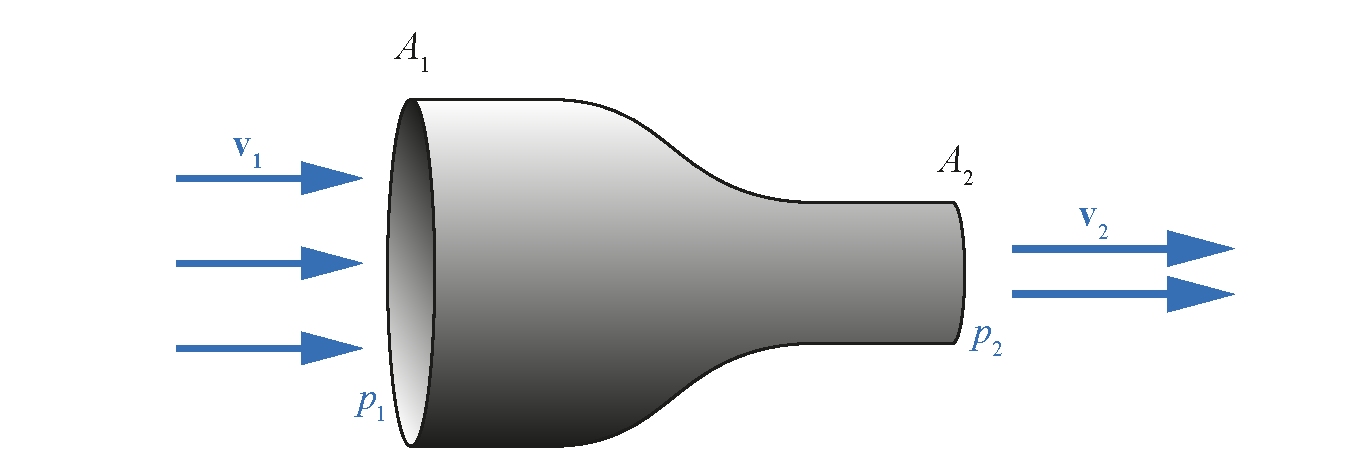
\includegraphics[width=\textwidth]{StroemungBernoulli.pdf}
  \caption[Zur Bernoulli-Gleichung]{Zur Bernoulli-Gleichung: Str�mung durch
    ein Rohr mit unterschiedlichen Querschnitten entlang der Koordinate $x$. Die Geschwindigkeit muss an
    den Querschnitten $A_1$ und $A_2$ in einer station�ren Str�mung einer
    inkompressiblen Fl�ssigkeit verschieden sein. Das hat Auswirkungen
    auf den Druck in den beiden Rohrbereichen.}
  \label{abb:kontmech_StroemungBernoulli}
\end{figure}

Damit die Geschwindigkeit unterschiedlich sein kann, muss das Gas jedoch entlang der Koordinate $x$
beschleunigt werden. Nach der Euler-Gleichung \eqref{eq:kontmech_EulerGleichung}
kann die Beschleunigung in Abwesenheit von �u�eren Kr�ften und Reibung
allein durch den Druck aufgebracht werden. Tats�chlich transportiert der
Druck $p$ die Fl�ssigkeit oder das Gas entlang des Weges $\D x$ durch das Rohr mit Querschnitt $A$ und
verrichtet dabei die Arbeit
\begin{equation}
  \Delta W = \Delta p \,A \,\D x = \Delta p \,\D V \; .
  \label{eq:kontmech_ArbeitBernoulli}
\end{equation}
Diese Arbeit f�hrt zur Beschleunigung und damit zur �nderung der kinetische
Energie.

Die Str�mung kommt mit dieser Erkl�rung dadurch zustande, dass ein
Massenelement von seinem nachfolgenden eine Kraft erf�hrt und diese an das
Massenelement vor ihm weitergibt. Ist der Rohrquerschnitt konstant, gleichen
sich diese Kr�fte gerade aus und die Geschwindigkeit bleibt konstant. Ein
Massenelement
\begin{equation}
  \D m = \varrho\,\D V \; ,
  \label{eq:kontmech_Massenelement}
\end{equation}
das gerade am �bergang zwischen den beiden Rohrabschnitten ist, wird im
Rohrabschnitt mit dem Querschnitt $A_1$ beschleunigt und beschleunigt selbst
ein weiteres Massenelement im Rohrabschnitt mit dem Querschnitt $A_2$. Diese
Arbeitsleistungen m�ssen unterschiedlich sein, damit eine �nderung der
kinetischen Energie auftreten kann. F�r eine inkompressible Fl�ssigkeit ist
$\varrho$ konstant und nach den Gleichungen \eqref{eq:kontmech_ArbeitBernoulli}
und \eqref{eq:kontmech_Massenelement} ist das nur m�glich, wenn der
Druck in beiden Rohrabschnitten unterschiedlich ist. Dieser l�sst sich sogar
aus der Energieerhaltung berechnen. Dazu stellen wir zun�chst fest, dass
die Differenz der kinetischen Energie des Gases im Rohrabschnitt mit dem Querschnitt $A_2$
und der im Abschnitt mit $A_1$ aus der Differenz der Arbeitsleitungen ergeben muss:
\begin{equation*}
  \Delta T = \frac{1}{2} \varrho \, \D V \, u_2^2 - \frac{1}{2} \varrho \, \D V \, u_1^2
  =  \Delta W = p_1 \,\D V - p_2 \,\D V = \Delta p \D V \,.
\end{equation*}
Dies l�sst sich zur \emph{Bernoulli-Gleichung}\index{Bernoulli-Gleichung}
\begin{equation}
  \frac{1}{2} \varrho \, u_1^2 + p_1 = \frac{1}{2} \varrho \, u_2^2 +  p_2
  \label{eq:kontmech_BernoulliGl}
\end{equation}
umformen. Die Konstante
\begin{equation}
  p_0 = \frac{1}{2} \varrho \, u^2 + p 
  \label{eq:kontmech_Staudruck}
\end{equation}
l�sst sich als der Druck interpretieren, den die Fl�ssigkeit ruhend (also
im Grenzfall eines unendlich breiten Rohres) annehmen w�rde. Der Druck $p$
ist der \emph{statische Druck der str�menden Fl�ssigkeit}\index{Druck!statischer}.
Die Bernoulli-Gleichung ist eine der Grundgleichungen f�r die Behandlung von Str�mungen in Fluiden und ist Grundlage vieler aero- und hydrodynamischer Berechnungen in der Technik. Sie wurde vom Sohn Daniel\indexp{Bernoulli, Daniel}\footnote{Daniel Bernoulli (1700 -- 1782) war ein Schweizer Mathematiker und Physiker, der eng mit Leonhard Euler zusammen arbeitete.} und Vater Johann Bernoulli\indexp{Bernoulli, Johann}\footnote{Johann Bernoulli (1667 -- 1748) war Schweizer Mathematiker und Arzt.
  Er arbeitete unter anderem auf dem Gebiet der Reihen und Differentialgleichungen.} aufgestellt.\\
Wir haben hier die Bernoulli-Gleichung aus energetischen �berlegungen (Energieerhaltung, da keine Reibung) hergeleitet. Man kann sie auch direkt aus der Euler-Gleichung \eqref{eq:kontmech_EulerGleichung} herleiten (\probref{kontmech_bernoulli}).

% BEISPIEL %%%%%%%%%%%%%%%%%%%%%%%%%%%%%%%%%%%%%%%%%%%%%%%%%%%%%%%%%%%%%%%%%%%%%%%%%%%%%%%%%%
\begin{example}{Schiff in einem Kanal}
\label{bsp:kontmech_SchiffKanal}
\smallskip

Der unterschiedliche statische Druck bei unterschiedlichen
Flie�geschwindigkeiten macht sich auch in der Schifffahrt bemerkbar. Im M�rz
2021 legte sich das Containerschiff "`Ever Given"' im Suezkanal quer und
blockierte diesen f�r mehrere Tage. Daf�r kann unter anderem der
Druckunterschied in str�menden Fl�ssigkeiten verantwortlich gemacht werden
\cite{Woehrbach2021}. Um dies darzustellen, soll
\figref{kontmech_SchiffKanalStroem} als Skizze dienen.

\begin{center}
  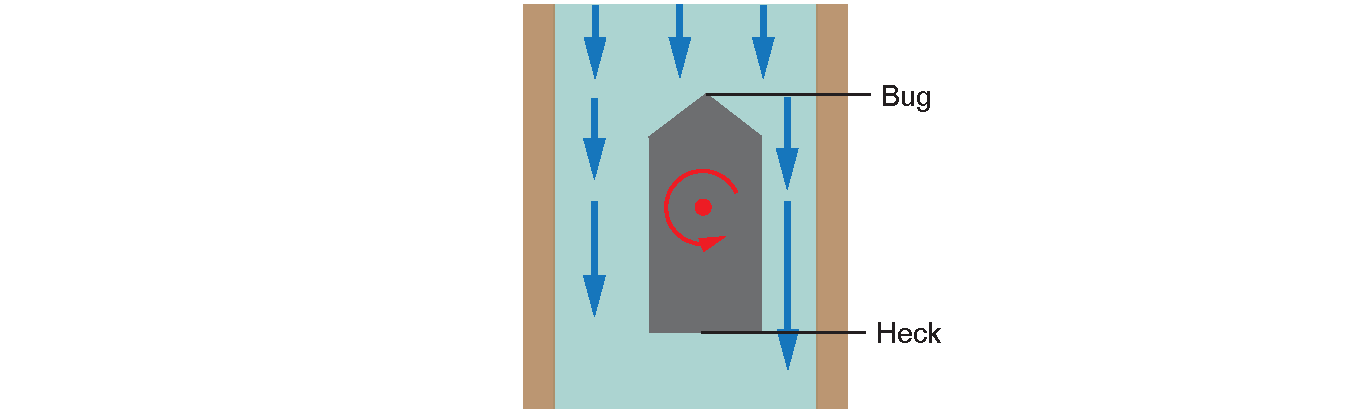
\includegraphics[width=\textwidth]{SchiffKanalStroem.pdf}
  \captionof{figure}{Str�mungen um ein Schiff in einem Kanal.}%
  \label{abb:kontmech_SchiffKanalStroem}
\end{center}

F�hrt das Schiff nicht in der Mitte des Kanals, muss das ausweichende Wasser an
beiden Seiten des Schiffes mit unterschiedlichen Geschwindigkeiten flie�en.
Dies bewirkt eine seitliche Kraft auf das Schiff. Durch die Form des Schiffes
gibt es aber auch einen Unterschied in den seitlichen Kr�ften zwischen Bug und
Heck des Schiffes, was in einem Drehmoment resultiert.
Im eingezeichneten Beispiel ist die Str�mungsgeschwindigkeit links vom Schiff
kleiner als rechts. Damit ist aber der statische Druck auf der linken Seite
gr��er als auf der rechten. Es resultiert eine Kraft nach rechts. Am Bug
sind die Str�mungsunterschiede geringer als am Heck. Das hei�t, die
resultierende Kraft ist am Heck gr��er als am Bug. Folglich wird sich das
Schiff mit dem Heck nach rechts drehen.
\probref{kontmech_SchiffKanal} besch�ftigt sich ausf�hrlicher mit einem
solchen Beispiel.
\end{example}
%BEISPIEL %%%%%%%%%%%%%%%%%%%%%%%%%%%%%%%%%%%%%%%%%%%%%%%%%%%%%%%%%%%%%%%%%%%%%%%%%%%%%%%%%%



\subsubsection{Innere Reibung}
\label{kap:kontmech_InnereReibung}\index{Reibung!innere}\index{Viskosit�t|textbf}

Wenn sich Fl�ssigkeiten und Gase bewegen, sto�en die einzelnen Atome
oder Molek�le aneinander und �bertragen dabei einen Impuls. Dies entspricht
einer inneren Kraftwirkung oder einer inneren Reibung. Um diese quantifizieren
zu k�nnen, betrachten wir die Situation aus \figref{kontmech_InnereReibung1}a.
Eine Fl�ssigkeit ist zwischen zwei Platten eingesperrt. Die rechte Platte
wird mit einer konstanten Geschwindigkeit $\vec{v}_0 = v_0\,\veceZ$ gegen die
linke verschoben. Dabei sp�rt man den Widerstand durch die innere Reibung.

\begin{figure}
  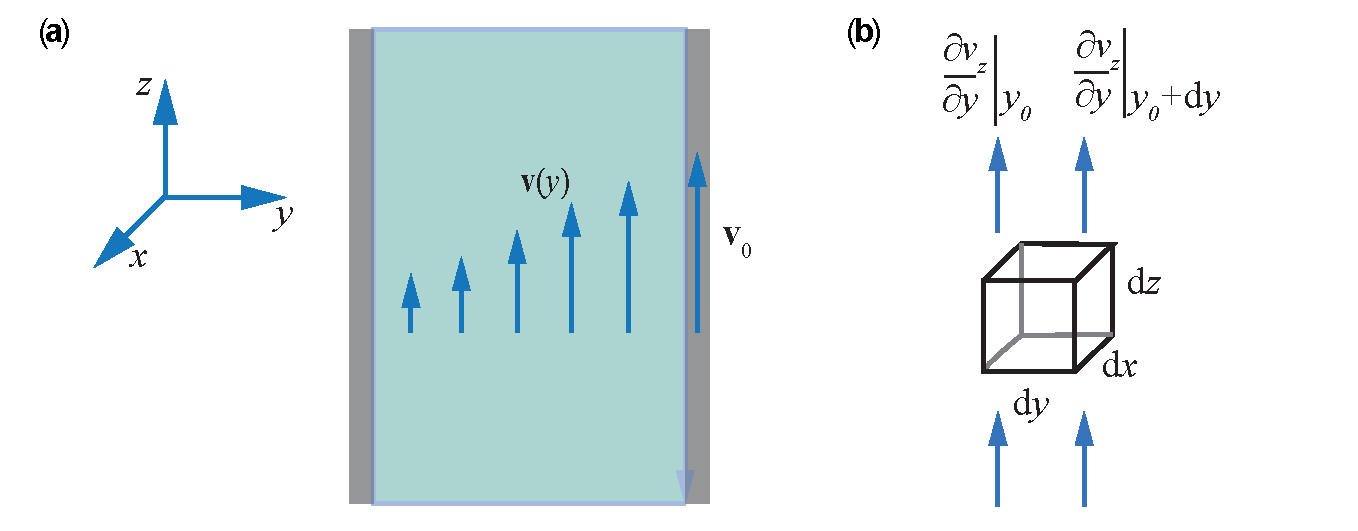
\includegraphics[width=\textwidth]{InnereReibung.pdf}
  \caption[Innere Reibung in einer Fl�ssigkeit]{\fa Eine Fl�ssigkeit ist
    zwischen zwei Platten eingespannt. Die rechte Platte wird mit $\vec{v}_0
    = v_0 \, \veceZ$ gegen die linke bewegt. In der Fl�ssigkeit bildet sich ein
    Geschwindigkeitsgradient aus. \fb F�r die Kraft auf ein Volumenelement
    $\D V = \D x\, \D y\, \D z$ m�ssen die Reibungen an allen Fl�chen beachtet
    werden. Hier werden sie bei $y_0$ und $y_0 + \D y$ unterschiedlich
    angenommen.}
  \label{abb:kontmech_InnereReibung1}
\end{figure}

Die Fl�ssigkeitsmolek�le sind an den R�ndern mit beiden
Platten in Kontakt und haben daher mit diesen die gleiche Geschwindigkeit. Innerhalb
der Fl�ssigkeit herrscht also ein Geschwindigkeitsgradient in $y$-Richtung.
Da die Kraftwirkung nur durch die Impuls�bertragung zwischen den
Fl�ssigkeitsmolek�len zustande kommen kann, k�nnen wir folgende Abh�ngigkeiten
voraussetzen:
\begin{itemize}
\item Die Kraft zwischen zwei Schichten der Fl�ssigkeit ist nach den
  Newtonschen Bewegungsgleichungen \eqref{eq:bew_NewtonBGL} proportional zur
  Impuls�nderung und damit zum Geschwindigkeitsgradienten.
\item Die Kraft muss proportional zur Zahl der sto�enden Molek�le sein. Diese
  ist jedoch, da sie (in einer Fl�ssigkeit immer, in einem Gas zumindest im
  Mittel) einen festen Raum einnehmen, proportional zur Fl�che $A$ der Grenze
  zwischen zwei Fl�ssigkeitsschichten. 
\end{itemize}
Wir erhalten f�r die Kraft
\begin{equation}
  \vec{F}_\text{R} = \eta \, A \, \frac{\partial v_z}{\partial y}
  \veceZ \; ,
  \label{eq:kontmech_ReibungskraftInnere}
\end{equation}
wobei wir den Proportionalit�tsfaktor $\eta$ als \emph{Viskosit�t}\glslink{viskositaet} bezeichnen\index{Viskosit�t}. Die Viskosit�t hat die Einheit
$\SI{}{\newton \second \per \metre^2}$ und beschreibt die
Eigenschaft der Fl�ssigkeit oder des Gases, Widerstand gegen eine
Bewegungs�nderung zu leisten.

Diese Kraft beschreibt bisher aber nur, welche Reibung an der Grenze zwischen
zwei Schichten der Fl�ssigkeit oder des Gases entsteht. Wollen wir die Kraft
wissen, die auf ein Volumen $\D V$ der Fl�ssigkeit wirkt, m�ssen wir uns
ein solches Fl�ssigkeitsvolumen herausschneiden, wie es in
\figref{kontmech_InnereReibung1}b eingezeichnet ist. Auf der rechten Seite
wird das Volumen von der angrenzenden Schicht beschleunigt, $\D V$ erf�hrt
also eine Kraft in positive $z$-Richtung. Auf der linken Seite ist es
das Volumenelement $\D V$ selbst, das die angrenzende Schicht beschleunigt und
dabei selbst eine Kraft in negative $z$-Richtung erf�hrt. Insgesamt ergibt
sich damit nach \eqref{eq:kontmech_ReibungskraftInnere} die Kraft
\begin{equation}
  \vec{F}_{\text{R},y} = \eta \lk {\frac{\partial v_z}
    {\partial x}}\big|_{y_0 + \D y} - {\frac{\partial v_z}{\partial y}}\big|_{y_0}
  \rk \,\veceZ \, \D x \, \D z\; .
\end{equation}
Liegen am linken und am rechten Rand identische Geschwindigkeitsgradienten vor,
sieht man sofort, dass das Volumenelement $\D V$ keine resultierende Kraft
erf�hrt. Im Allgemeinen ist das aber nicht der Fall. Sehr sicher k�nnen wir
 davon ausgehen, dass wir f�r den differentiellen Abstand $\D y$ eine
Linearisierung des Gradienten durchf�hren k�nnen. Wir setzen also an:
\begin{equation}
  \frac{\partial v_z}{\partial y}\big|_{y_0 + \D y} =
  \frac{\partial v_z}{\partial y}\big|_{y_0} + \frac{\partial^2 v_z}
  {\partial y^2}\big|_{y_0}  \D y \; . 
\end{equation}
F�r die Kraft auf das Volumenelement ergibt sich somit
\begin{subequations}
  \begin{align}
    \vec{F}_{\text{R},y} &= \eta \lk \killA{\frac{\partial v_z}
      {\partial y}\big|_{y_0}} +  \frac{\partial^2 v_z}{\partial y^2}\big|_{y_0} \D y
      - \killA{\frac{\partial v_z}{\partial y}\big|_{y_0}} \rk \, \veceZ\, \D x \, \D z 
    = \eta \, \frac{\partial^2 v_z}{\partial y^2}\big|_{y_0}\, \veceZ\, \D V \; .
    %&= \eta \, \frac{\partial^2 v_z}{\partial y^2}\big|_{y_0 }\, \veceZ\,\D x \, \D y \, \D z
  \end{align}
  Vollkommen analog �berlegt man sich, dass bei einem vorhandenen
  Geschwindigkeitsgradienten in $x$-Richtung gilt, dass
  \begin{equation}
    \vec{F}_{\text{R},x} = \eta \, \frac{\partial^2 v_z}
    {\partial x^2}\big|_{y_0}\,\veceZ\, \D V \; .
  \end{equation}
\end{subequations}
Ist die Bewegung einer inkompressiblen Fl�ssigkeit nicht entlang der
$z$-Richtung ausgerichtet, sondern besitzt sie auch zumindest eine Komponente
in $x$- oder $y$-Richtung, so ist dieselbe �berlegung f�r einen Gradienten
(bzw. einen sich �ndernden Gradienten) in $z$-Richtung m�glich.\footnote{Ein
Geschwindigkeitsgradient in $z$-Richtung tritt nat�rlich auch bei Str�mungen
mit sich �ndernden Querschnitten (siehe \kap{kontmech_BernoulliGl})
oder bei kompressiblen Fl�ssigkeiten auf, wenn die Bewegung allein in
$y$- \bzw $z$-Richtung erfolgt.} Im allgemeinen Fall erh�lt man mit dem
Laplace-Operator \eqref{eq:kontmech_laplace_eq}
\begin{equation*}
  \Delta = \frac{\d^2}{\d x^2} + \frac{\d^2}{\d y^2} + \frac{\d^2}{\d z^2} 
\end{equation*}
f�r die gesamten Kr�fte, die sich durch die Reibung der Schichten aneinander
auf das Volumenelement $\D V$ ergeben
\begin{align}
  \vec{F}_{\text{R}} &= \eta \, \Delta \vec{v}\big|_{(x_0, y_0, z_0)} \, \D V
  = \eta \, \Delta \vec{v}\big|_{\vec{r}_0} \, \D V ~~~\text{\bzw}~~~ \vec{f}_{\text{R}} = \eta \, \Delta \vec{v}\big|_{\vec{r}_0} \; .
\label{eq:kontmech_InnereReibung}
\end{align}

\subsection{Navier-Stokes-Gleichung}
\label{kap:kontmech_NavierStokes}\index{Navier-Stokes-Gleichung|textbf}

Nachdem wir nun einzelnen Kraftterme auf Basis der Euler-Gleichung untersucht und insbesondere die innere
Reibung eines Fluids gekl�rt haben, k�nnen wir die erhaltenen Beziehungen
in die Euler-Gleichung \eqref{eq:kontmech_EulerGleichung} \bzw \eqref{eq:kontmech_WellenEulerGleichung} einsetzen. Mit
der Druckkraft \eqref{eq:kontmech_Druckkraft} und der inneren Reibungskraft
\eqref{eq:kontmech_InnereReibung} erh�lt man dann die \emph{Navier-Stokes-Gleichung}
\begin{equation}
  \varrho \lk \lk \vec{v} \cdot \nablav \rk \vec{v} + \frac{\partial}{\partial t}
  \vec{v} \rk = \vec{f}_\text{V}  + \eta \, \Delta \vec{v} - \nablav p \; ,
  \label{eq:kontmech_NavierStokes}
\end{equation}
in der nur noch die Kraftdichte $\vec{f}_\text{V}$ der von au�en wirkenden
Volumenkr�fte nicht explizit gegeben sind. Sie ist eine partielle Differentialgleichung in $\vec{v}(\vec{r},t)$ bei gegebenen externen Kr�ften $ \vec{f}_\text{V}$ und statischen Druck $p$. 
%Letztere h�ngen nat�rlich von der Wechselwirkung mit der Umgebung ab. 
Wir m�chten darauf hinweisen, dass die \NVS \eqref{eq:kontmech_NavierStokes} in der Form \eqref{eq:kontmech_NavierStokes}
nur f�r inkompressible Fluide gilt. Es gibt auch eine \NVS f�r kompressible Fluide, die noch etwas komplizierter ist. Wir verweisen dazu auf \cite{Garvin2023}.
Wie bei jeder PDGL m�ssen die Randbedingungen f�r das betrachtete Volumen ber�cksichtigt werden. Die Navier\footnote{Claude Louis Marie Henri Navier (1785 -- 1836) war ein franz�sischer Mathematiker, Bauingenieur und Physiker. Er brachte die Elastizit�tstheorie in eine mathematisch handhabbare Form und gilt auch als Begr�nder der Baustatik. 1822 gab er die Navier-Stokes-Gleichungen f�r die Bewegung einer viskosen Fl�ssigkeit an.}\indexp{Navier, Claude Louis Marie Henri}-Stokes
%\footnote{Sir George Gabriel Stokes\indexp{Stokes, Sir George Gabriel} (1819--1903) war ein irischer Mathematiker und Physiker. Er arbeitete auf dem Gebiet der mathematischen und experimentellen Physik und besch�ftigte sich haupts�chlich mit der Hydrodynamik, der Elektrodynamik und der Akustik.}
-Gleichung\indexp{Stokes, Sir George Gabriel} ist damit eine Spezifizierung der Euler-Gleichung der Kontinuumsmechanik bez�glich der inneren Reibung und insbesondere der Einf�hrung der Viskosit�t.
Die partielle Differentialgleichung stellt eine gro�e mathematische Herausforderung dar, es ist nicht bekannt, ob es f�r den allgemeinen dreidimensionalen Fall eine �berall definierte (eindeutige) L�sung gibt. Die Frage nach der L�sung dieser Gleichung in ihrer allgemeiner Form  geh�rt daher zu den gro�en ungel�sten mathematischen Problemen und stellt eines der sogenannten sieben Millennium-Probleme\footnote{Als Millennium-Probleme wurden im Jahr 2000 durch das \textit{Clay Mathematics Institute (CMI)} in Cambridge (Massachusetts, USA) sieben ungel�ste mathematische Problem in einer Liste zusammen gefasst. F�r die L�sung eines der sieben Probleme wurde jeweils ein Preisgeld von einer Million US-Dollar ausgelobt.} dar.\\
Drei generelle Bemerkungen seien zur \NVS noch gemacht.
\begin{itemize}
	\item Die dominante, \dh gesuchte Variable in der \NVS ist der Geschwindigkeitsvektor $\vec{v}$. Der Druck ist \ia ebenfalls unbekannt, w�hrend wie erw�hnt die Dichte (f�r die inkompressible Fl�ssigkeit) und die externen Kr�fte als bekannt angenommen werden k�nnen. Die \NVS ist eigentlich in Komponenten geschrieben ein Set von drei Gleichungen. Wir haben aber vier Unbekannte, die 3 Komponenten der Geschwindigkeit (als Funktion von Ort und Zeit) und den Druck. Die dazu notwendige vierte Gleichung ist die Kontinuit�tsgleichung \eqref{eq:kontmech_KontinuitaetsglDiff}, die f�r die inkompressible Fl�ssigkeit durch $\nablav \vec{v} = 0$ gegeben ist.  
	\item Der Druck taucht in der Gleichung nur in Form $\nablav p$ auf. Das bedeutet, dass die Dynamik von inkompressiblen Fluiden immer nur von Druckdifferenzen abh�ngt und nicht von den Absolutwerten des Drucks, was relativ einsichtig ist.
	\item Wegen des Terms $\lk \vec{v} \cdot \nablav \rk \vec{v}$ ist die Differentialgleichung nichtlinear, dieser Term stellt die eigentliche Schwierigkeit in der L�sung der DGL dar.
\end{itemize}
Zwei wichtige l�sbare Spezialf�lle der Navier-Stokes-Gleichung sollen aber explizit genannt werden, zum einen der Fall, in dem jegliche von au�en angreifende Volumenkr�fte fehlen,
\begin{subequations}
  \begin{align}
    \varrho \lk \lk \vec{v} \cdot \nablav \rk \vec{v} + \frac{\partial}
    {\partial t} \vec{v}  \rk &= \eta \, \Delta \vec{v} - \nablav p \; ,
              \label{eq:kontmech_NavierStokesFrei} \\
    \intertext{und zum anderen der Fall, in dem eine Fl�ssigkeit oder ein Gas sich im homogenen Gravitationsfeld befindet, welches eine Kraftdichte $\varrho\,\vec{g}$ hat} 
    \varrho \lk \lk \vec{v} \cdot \nablav \rk \vec{v} + \frac{\partial}
    {\partial t} \vec{v} \rk &= \varrho\,\vec{g} + \eta \, \Delta \vec{v}
                               - \nablav p \; .
              \label{eq:kontmech_NavierStokesSchwerefeld}
  \end{align}
\end{subequations}



% BEISPIEL %%%%%%%%%%%%%%%%%%%%%%%%%%%%%%%%%%%%%%%%%%%%%%%%%%%%%%%%%%%%%%%%%%%%%%%%%%%%%%%%%%
\begin{example}{�berlegungen zu Str�mungen anhand des Stra�enverkehrs}
  \label{bsp:VerkehrKreuzung}
  \smallskip
  Wie bereits erw�hnt werden Methoden der Kontinuumsmechanik in vielen anderen Gebieten zur Problembeschreibung und -l�sung verwendet.
	Angeregt von einer Aufgabe in \cite{Meschede2010} m�chten wir uns zum
  Abschluss des Abschnitts ein Beispiel zur Kinematik und Dynamik des
  Stra�enverkehrs geben und zeigen wie auch in diesem Gebiet Begriffe aus der Kontinuumsmechanik, wie Str�mungen \usw verwendet werden k�nnen und damit auch veranschaulicht werden.
	Selbstverst�ndlich
  lassen sich viele weitere analoge Bilder finden. Wir m�chten insbesondere folgende
  heranziehen:

\begin{itemize}
\item \textbf{Beispiele f�r Strom- und Bahnlinien.}\\
  Stromlinien lassen sich aus den momentanen Geschwindigkeiten der Autos
  im Stra�enverkehr bilden. Wir m�ssen diese ermitteln und Linien einzeichnen,
  die tangential an diesem Feld liegen. Bahnlinien sind die tats�chlich
  gefahrenen Wege der einzelnen Autos. In einem station�r flie�enden Verkehr sind Strom-
  und Bahnlinien identisch, auf einspurigen Stra�en ohne Abzweigungen sind sie
  das sogar immer. Sie unterscheiden sich, wenn ein Auto spontan beschleunigt. Das
  kann \zb bei einem Spurwechsel ober beim Abbiegen an einer Kreuzung der Fall
  sein.
  
\item \textbf{Messen des Flusses.}\\
  Den Fluss bestimmt man, indem man die Autos z�hlt, die einen Querschnitt der
  Stra�e in einem festen Zeitintervall durchqueren.

\item \textbf{Kompressibilit�t und Inkompressibilit�t der Fahrzeugstr�mung.}\\
  In einem station�r flie�enden Verkehr ist die Fahrzeugstr�mung immer
  inkompressibel. Am Stauende einer Autobahn oder vor einer roten Ampel an
  einer Kreuzung hingegen verdichten sich die Autos. Hinter einer Verengung (z.B. auf
  einer Autobahn hinter einer Baustelle) beschleunigen sie wieder. Im
  Allgemeinen ist der Stra�enverkehr (Autodichte) also kompressibel.
  
\item \textbf{Divergenz- und Rotationsfreiheit. Beispiele f�r Quellen und
    Senken.}\\
  Divergenzfrei w�rde bedeuten, es k�nnen nie mehr oder weniger Autos im
  Verkehr werden. Global betrachtet stimmt das, aber definitiv nicht f�r
  eine einzelne Stra�e. Eine Autobahnausfahrt ist eine Senke, eine Auffahrt
  eine Quelle f�r Autos auf der Autobahn. Entsprechend k�nnen im Stadtverkehr
  an einer Kreuzung Autos von der Hauptstra�e abfahren (Senke f�r den Verkehr
  auf der Hauptstra�e) oder auf sie auffahren (Quelle).

  Rotationsfrei ist der Verkehr \iA ebenfalls nicht. Neben dem
  Kreisverkehr gibt es aber auch weitere Beispiele. Eine Rotation liegt
  bereits dann vor, wenn auf einer mehrspurigen Stra�e nicht auf allen
  Spuren gleich schnell gefahren wird. Auf einer Autobahn ist das, bis auf
  Ausnahmen wie \zb dichter Verkehr, immer der Fall.
  
\item \textbf{Beispiele f�r beide Terme der materiellen Beschleunigung.}\\
  Die Geschwindigkeit eines Autos h�ngt nat�rlich vom Geschwindigkeitsfeld
  des Verkehrs ab. Stellen wir uns eine Stra�e vor, auf der in verschiedenen
  Abschnitten unterschiedliche Geschwindigkeiten gelten, \zb $\SI{30}{\kilo
    \metre \per \hour}$ vor einer Schule, sonst $\SI{50}{\kilo
    \metre \per \hour}$. Vor der Schule bremsen alle Autos, dahinter
  beschleunigen sie. Das entspricht dem ersten Term der materiellen
  Beschleunigung in \eqref{eq:kontmech_Beschleunigung}, der beschreibt, dass ein Auto in ein anderes
  Geschwindigkeitsfeld ger�t. Ein einzelnes Auto, dessen Fahrer es eventuell
  eilig hat, kann ein anderes vor der Schule �berholen. Es weicht von der
  Geschwindigkeit aller Autos ab und wird einzeln beschleunigt. Das entspricht
  dem zweiten Term in Gleichung \eqref{eq:kontmech_Beschleunigung}.
  
\item \textbf{Analoga zu den Termen der Navier-Stokes-Gleichung.}\\
  In der Navier-Stokes-Gleichung tritt die materielle Beschleunigung auf
  (siehe oben). Diese wird von innerer Reibung beeinflusst. In der
  Annahme, dass wir keine Unf�lle haben, sich die Autos also nicht ber�hren,
  wird die innere Reibung dadurch gegeben, dass ein Auto nicht mit anderen
  zusammensto�en m�chte und \zb hinter einem langsamer werdenden Auto
  abbremsen muss, um nicht auf dies aufzufahren. Dies entspricht dem
  Viskosit�tsterm. Der Druckgradient entspricht z.B. einer roten Ampel (h�herer
  Druck vor dem Auto) oder einer gr�nen Ampel (niedrigerer Druck vor dem Auto).
	�u�ere Kr�fte k�nnen z.B. Hangabtriebskr�fte auf einer Strecke mit
  Steigung oder Gef�lle sein.   
  \end{itemize}

\end{example}
%BEISPIEL %%%%%%%%%%%%%%%%%%%%%%%%%%%%%%%%%%%%%%%%%%%%%%%%%%%%%%%%%%%%%%%%%%%%%%%%%%%%%%%%%%

Wir verweisen am Ende dieses Kapitels noch einmal auf Tabelle \ref{tab:kontmech_stroemung_overview}, in der wir die verschiedenen Str�mungsarten zusammengefasst haben. Wir wollen uns daran anschlie�end etwas n�her mit dem Spezialfall der laminaren Str�mungen besch�ftigen.
\begin{table}
\caption[�bersicht der verschiedenen Str�mungsarten.]{�bersicht der verschiedenen Str�mungsarten.}
\begin{tabular}{L{3cm}L{4.5cm}L{4.5cm}}
  \hline\noalign{\smallskip}
  Charakterisierung &  &    \\
  \noalign{\smallskip}\svhline\noalign{\smallskip}
	nach innerer Reibung&ideal Fluide\index{Fluid!ideales}, ohne innerer Reibung \linebreak $\eta =0$ &reale Fluide\index{Fluid!reales}, mit innerer Reibung \linebreak $\eta \neq 0$\\
\rule{0pt}{1pt}\\
	nach Kompressibilit�t&inkompressibel \linebreak  $\varrho = \con$ &kompressibel \linebreak  $\varrho \neq \con$ \\
\rule{0pt}{1pt}\\
	nach Wirbelfreiheit&wirbelfrei, laminar \linebreak  $\rotv \vec{v} = 0$ & verwirbelt\linebreak  $\rotv \vec{v} \neq 0$  \\
\rule{0pt}{1pt}\\
	nach Quellenfreiheit&quellenfrei \linebreak $\divv \vec{v} = 0$ &mit Quellen und Senken \linebreak $\divv \vec{v} \neq  0$\\
\rule{0pt}{1pt}\\
	nach zeitlichem Verhalten &station�r \linebreak  $\d \vec{v}/ \d t  = 0$&nicht-station�r \linebreak  $\d \vec{v}/ \d t  \neq 0$ \\
\rule{0pt}{1pt}\\
	Potentialstr�mung&quellenfrei, wirbelfrei \linebreak $\vec{v} = -\gradv \varphi$ &\\
\noalign{\smallskip}\hline\noalign{\smallskip}
\end{tabular}
\label{tab:kontmech_stroemung_overview}
\end{table}


\clearpage
\section{Bewegungen von Fl�ssigkeiten und Gasen}\label{kap:kontmech_fluide}
\index{Fl�ssigkeiten}\index{Gase}
Wir wollen uns nun einige Spezialf�lle der \NVS genauer anschauen. Uns interessieren dabei vor allem die Str�mungsprofile,
die sich durch die Reibung ergeben.

\subsection{Laminare Str�mungen inkompressibler
  Fl�ssigkeiten}
\label{kap:kontmech_laminareStroemungenFluessigkeiten}
\index{Str�mung!laminar}

Zun�chst m�chten wir uns mit dem relativ einfachen Fall der
Fluiddynamik besch�ftigen, den \emph{laminaren Str�mungen
in inkompressiblen Fl�ssigkeiten} mit konstanter Geschwindigkeit. 

Um die Str�mungsprofile (wir erinnern uns, dass ein Str�mungsprofil durch $\vec{v}(\vec{r},t)$ 
beschrieben wird) zu bestimmen, gehen wir von der Navier-Stokes-Gleichung
\eqref{eq:kontmech_NavierStokesFrei} ohne von au�en wirkende Volumenkr�fte $\vec{f}_\text{V}$ aus.
Wir gehen ferner von einem konstanten Querschnitt der Str�mung aus und legen das
Koordinatensystem so, dass die Geschwindigkeit $\vec{v}$ in Richtung von
$\veceZ$ erfolgt. Der konstante Querschnitt erzwingt zusammen mit der
Massenerhaltung und der Inkompressibilit�t, dass sich die Geschwindigkeit in
$z$-Richtung nicht �ndern kann, es gilt also $\vec{v} = v_z(x,y)\, \veceZ$.
Daraus folgt f�r den ersten Term auf der linken Seite der
Navier-Stokes-Gleichung \eqref{eq:kontmech_NavierStokesFrei}, dass
\begin{equation*}
  \left ( \vec{v} \cdot \nablav \right ) \vec{v} =  \left ( v_z(x,y)\,\veceZ
    \cdot \nablav \right ) v_z(x,y) \,\veceZ
  =  \left (v_z(x,y) \frac{\partial}{\partial z}  \right ) v_z(x,y)\, \veceZ
    = \vec{0} \; .
\end{equation*}
F�r eine station�re Str�mung gilt weiterhin, dass $\partial \vec{v}/\partial t	
=0$. Somit reduziert sich die Navier-Stokes-Gleichung auf ein Gleichgewicht von
Druckkraft und  Reibung:
\begin{equation}
  \eta \, \Delta \vec{v} - \nablav p = \vec{0} \; .
  \label{eq:kontmech_NaStstat}
\end{equation}
Im folgenden Beispiel wollen wir diese Differentialgleichung f�r zwei
sehr einfache Geometrien l�sen.

%BEISPIEL %%%%%%%%%%%%%%%%%%%%%%%%%%%%%%%%%%%%%%%%%%%%%%%%%%%%%%%%%%%%%%%%%%%%%%%%%%%%%%%%%%
\begin{example}{Station�re laminare Str�mungen in einfachen Profilen}
\label{bsp:kontmech_laminareStroemungen}\index{Str�mung!laminare}
\smallskip

In diesem Beispiel wollen wir die Differentialgleichung
\eqref{eq:kontmech_NaStstat} f�r station�re Str�mungen in zwei sehr einfachen
Geometrien l�sen, um einen ersten Eindruck zu bekommen, wie solche
L�sungen aussehen k�nnen. Zun�chst gehen wir von einer Situation aus, die
\figref{kontmech_InnereReibung1}a sehr �hnlich ist. Wir wollen jetzt
jedoch annehmen, dass die Berandung auf beiden Seiten unbeweglich ist. Die
Str�mung wird durch ein Druckgef�lle angetrieben und wir gehen davon aus,
dass sie sich station�r eingestellt hat, sodass \eqref{eq:kontmech_NaStstat}
gilt. Wenn wir zus�tzlich davon ausgehen, dass die Form des Randes in
$x$-Richtung so tief ist, dass ihre R�nder im betrachteten Teil der Str�mung
keinen Einfluss haben, k�nnen wir folgende Annahmen treffen.
\begin{itemize}
\item Die station�re Str�mung findet nur in Richtung $\veceZ$ statt. Es gilt
  also $\vec{v} = v_z \veceZ$.
\item Aus Symmetriegr�nden erwarten wir, dass der Druck ausschlie�lich
  von $z$ abh�ngt. Andernfalls w�rden nach \eqref{eq:kontmech_NaStstat} sofort
  Str�mungen in den Richtungen $\veceX$ und $\veceY$ auftreten, die diese
  Druckdifferenzen ausgleichen. Es gilt also $p=p(z)$.
\item Die Materieerhaltung in der inkompressiblen Fl�ssigkeit erzwingt , dass
  $v_z$ nicht von $z$ abh�ngt. Die Geschwindigkeit muss in jedem Rohrabschnitt
  dieselbe sein. Da wir nach Voraussetzung auch keinen Einfluss der Berandung
  in $x$-Richtung haben, gilt $v_z = v_z(y)$.  
\end{itemize}
Mit diesen �berlegungen reduziert sich Gleichung  \eqref{eq:kontmech_NaStstat}
zu
\begin{align*}
  \eta \, \frac{\partial^2}{\partial y^2} v_z(y)\, \veceZ - \frac{\partial p}
  {\partial z}\, \veceZ
  &= \vec{0} \quad \text{bzw.} \quad 
    \eta \, \frac{\partial^2}{\partial y^2} v_z(y)
  = \frac{\partial p}{\partial z} \,.
\end{align*}
Aus dieser Differentialgleichung l�sst sich f�r einen gegebenen Druckgradienten 
$p(z)$ eine formale L�sung f�r das Str�mungsprofil $v_z(y)$ finden,
\begin{equation*}
  v_z(y) = \frac{1}{2\eta} \frac{\partial p(z)}{\partial z}\,y^2 + \alpha y + \beta \,.
\end{equation*}
Aus den Randbedingungen $v_z(y=0) = v_z(b) = 0$ findet man $\beta=0$ und
\begin{equation*}
  \alpha = - \frac{b}{2\eta} \frac{\partial p(z)}{\partial z} 
~~~\text{sowie}~~~
  v_z(y) = \frac{1}{2\eta} \frac{\partial p}{\partial z} \left ( \left ( y^2 -
    \frac{b}{2} \right )^2 -\frac{b^2}{4} \right ) \; .
\end{equation*}
Dies ist eine nach unten offene Parabel mit dem Scheitel in der Mitte zwischen
den beiden W�nden und der maximalen Geschwindigkeit
\begin{equation}
  v_\text{max} = - \frac{1}{2\eta} \frac{\partial p(z)}{\partial z}
  \frac{b^2}{4}  \; .
\end{equation}
Die Str�mungsgeschwindigkeit nimmt also von der Mitte zum Rand hin quadratisch
ab. Sie h�ngt proportional von der Druckdifferenz $\partial p(z) / \partial z$ 
und der Breite der Str�mung $b$ ab und ist umgekehrt proportional zu der
Viskosit�t.\\

Ganz �hnlich l�sst sich die Str�mung durch ein kreisrundes Rohr \index{Str�mung!Rohr} mit dem
Radius $R$ beschreiben.
Wir gehen erneut davon aus, dass sie nur in $z$-Richtung erfolgt. Dann wird
auch der Druck weiterhin nur von $z$ abh�ngen. Die Symmetrie erfordert nun,
dass die Str�mung allein vom Abstand zum Mittelpunkt des Rohrquerschnitts
abh�ngt. In Zylinderkoordinaten l�sst sich das durch $v_z = v_z(r)$
beschreiben. Die Navier-Stokes-Gleichung \eqref{eq:kontmech_NaStstat} f�r
den station�ren Fall nimmt dann in Zylinderkoordinaten\index{Zylinderkoordinaten} die Form
\begin{equation*}
  \eta \, \frac{1}{r} \frac{\partial}{\partial r} \left ( r\,
    \frac{\partial v_z(r)}{\partial r} \right ) = \frac{\partial p(z)}{\partial z}
\end{equation*}
an. Die allgemeine L�sung dieser Differentialgleichung lautet
\begin{equation*}
  v_z(r) = \frac{1}{4\eta} \frac{\partial p}{\partial z} r^2 + \alpha \ln r
  + \beta
\end{equation*}
Damit die Str�mungsgeschwindigkeit im Ursprung endlich bleibt, muss $\alpha =
0$ gelten. Die Forderung, dass am Rand des Rohrs keine Str�mung stattfindet, 
$v_z(R) = 0$, ergibt schlie�lich
\begin{equation*}
  \beta = - \frac{R^2}{4\eta} \frac{\partial p(z)}{\partial z} 
\end{equation*}
und die Str�mungsgeschwindigkeit
\begin{equation}
  v_z(R) = \frac{1}{4\eta} \frac{\partial p(z)}{\partial z} \left ( r^2 - R^2
  \right ) \; .
  \label{eq:kontmech_StroemungsGeschwKreisrohr}
\end{equation}
Auch hier ist das Str�mungsprofil also parabelf�rmig. Die maximale
Str�mungsgeschwindigkeit lautet
\begin{equation*}
  v_\mathrm{max}  = v_z(0) = -\frac{1}{4\eta} \frac{\partial p(z)}{\partial z} R^2
  \; .
\end{equation*}
Sie steigt also bei konstanter Druckdifferenz quadratisch mit dem Rohrquerschnitt an.

\end{example}
%BEISPIEL %%%%%%%%%%%%%%%%%%%%%%%%%%%%%%%%%%%%%%%%%%%%%%%%%%%%%%%%%%%%%%%%%%%%%%%%%%%%%%%%%%

Die Beziehung \eqref{eq:kontmech_StroemungsGeschwKreisrohr} wird auch das Gesetz von Hagen\footnote{Gotthilf Heinrich Ludwig Hagen (1797--1884) war ein deutscher Wasserbauingenieur und Hochschullehrer. Er gab das erste in deutscher Sprache erschienene Handbuch der Wasserbaukunst heraus.}\indexp{Hagen, Gotthilf Heinrich Ludwig}-Poiseuille\footnote{Jean L�onard Marie Poiseuille (1797--1869) war ein franz�sischer Physiologe und Physiker. Er arbeitete vorwiegend auf dem Gebiet der Physiologie des Blutkreislaufs und versuchte physikalische  Erkenntnisse auf die Physiologie zu �bertragen.}\indexp{Poiseuille, Jean L�onard Marie}\index{Gesetz von Hagen-Poiseuille} genannt. Es beschreibt den Zusammenhang zwischen der Geschwindigkeit einer laminaren station�ren Str�mung bei einer dynamischen Viskosit�t $\eta$ in einem kreiszylindrischen Rohr mit dem Radius $R$ und bei einem Druckgradienten �ber die L�ngskoordinate der Str�mung.

In komplizierteren Geometrien gestaltet sich das Finden von L�sungen meist deutlich
schwieriger. Der Spezialfall \eqref{eq:kontmech_NaStstat}
der Navier-Stokes-Gleichung l�sst sich jedoch leicht numerisch l�sen. Die Partial
Differential Equation Toolbox von \matlab{} h�lt entsprechende
L�sungsverfahren bereit, die leicht zu bedienen sind. Ein Beispiel betrachten
wir in \probref{kontmech_StroemungRechteckrohr}, in der wir das
Geschwindigkeitsprofil einer laminaren, station�ren Str�mung in einem rechteckigen Rohr l�sen.


\subsection{Wirbel in Str�mungen (Turbulenz)}
\index{Wirbel!Str�mung}\index{Str�mung!turbulente}\index{Turbulenz}\index{Str�mung!Wirbel}

Nun wollen wir uns mit dem komplexeren Fall der
Fluiddynamik besch�ftigen, dem Auftreten von Wirbeln in Str�mungen, insbesondere bei kleinen oder verschwindenden inneren Reibungen. 
Wir behalten aber die Annahme 
inkompressibler Fluide bei. 
In \kap{kontmech_FormenStroemungen} haben wir bereits
gesehen, dass die Vektorgr��e Rotation $\rotv \vec{v}$ 
eine Str�mung charakterisiert.
Besondere Bedeutung hat dies, wenn eine Str�mung Wirbel aufweist. Wirbel
entstehen insbesondere, wenn Hindernisse von Fl�ssigkeiten oder Gasen
umstr�mt werden und die Reibung relativ gering ist.

Um uns dem Konzept der Wirbel mathematisch zu n�hern, betrachten wir zun�chst den einfachsten
Fall einer konstanten kreisf�rmigen Str�mung mit konstanter
Winkelgeschwindigkeit $\vec{\omega} =\conv$. In dieser verh�lt sich die Str�mung wie
ein starrer K�rper und man k�nnte erwarten, dass das f�r Fluide eine
unrealistische Beschreibung ist. Tats�chlich ist dies jedoch ein recht
zutreffender Fall, da sich typischerweise das Innere eines Wirbels, der
sogenannte Wirbelkern, genau so verh�lt wie ein starrer K�rper. Wir k�nnen
einen solchen Wirbel durch den Geschwindigkeitsvektor $\vec{v}$ beschreiben:
\begin{equation*}
  \vec{v}(\vec{r}) = \vec{\omega} \times \vec{r} .
\end{equation*}
Damit die Winkelgeschwindigkeit an jedem Ort konstant sein kann, muss die
Geschwindigkeit linear mit dem Abstand $|\vec{r}|$ vom Zentrum des Wirbels
ansteigen. Die Winkelgeschwindigkeit k�nnen wir wiederum f�r diesen Wirbel
aus
\begin{align}
  \frac{1}{2}\, \rotv \vec{v}
  &= \frac{1}{2}\, \rotv \lk \vec{\omega} \times \vec{r} \rk = \frac{1}{2} \,\nablav \times \lk  \vec{\omega} \times \vec{r} \rk \\
  &= \frac{1}{2} \, \left (
    \underbrace{\vec{\omega} \lk \nablav \cdot \vec{r} \right )}_{=3\vec{\omega}}
  - \vec{r} \underbrace{\left ( \nablav \cdot \vec{\omega} \right )}_{=0}
  + \underbrace{\left ( \vec{r} \cdot \nablav \right ) \vec{\omega}}_{=0}
  - \underbrace{\left ( \vec{\omega} \cdot \nablav \right ) \vec{r}
  }_{=\vec{\omega}} \rk
  = \vec{\omega}
\end{align}
erhalten. Bei der Rechnung haben wir \eqref{eq:kontmech_nablaop02} aus \kap{kontmech_VektorAnalysis} benutzt.\\
Im allgemeinen Fall $\vec{\omega} = \vec{\omega}(\vec{r})$ kann $\vec{\omega}$ nat�rlich an jedem
Ort unterschiedlich ausfallen. Um auch solche Str�mungen beschreiben zu k�nnen,
wird der \emph{Wirbelvektor}\index{Wirbelvektor} als die H�lfte der Rotation der Geschwindigkeit,
\begin{equation}
  \vec{\Omega} = \frac{1}{2} \rotv \vec{v} \; ,
  \label{eq:kontmech_Wirbelvektor}
\end{equation}
eingef�hrt. Im Fall des gerade beschriebenen einfachen Wirbels ist der Wirbelvektor mit dem Vektor der
Winkelgeschwindigkeit identisch.

Als weiteres Ma� f�r die St�rke eines Wirbels wird die \emph{Zirkulation}\index{Zirkulation!Str�mung}\index{Str�mung!Zirkulation}
\begin{equation}
  Z = \oint_{\partial A} \vec{v} \cdot \D\vec{s}
  = \int_{A} \rotv \vec{v} \cdot \D \vec{A} = 2\, \int_{A} \vec{\Omega} \cdot \D \vec{A}\; ,
  \label{eq:kontmech_Zirkulation}
\end{equation}
eingef�hrt, die sich nach dem Integralsatz von Stokes (siehe \eqref{eq:kontmech_Integralsatz_Stokes} in \kap{kontmech_Integralsaetze}) entweder als Wegintegral entlang des
Randes $\partial A$  der durchstr�mten Fl�che $A$ oder als Oberfl�chenintegral mit dem
orientierten Fl�chenelement $\D\vec{A}$ berechnen l�sst. Man beachte, dass
die Rotation $\rotv \vec{v}$ auch hier wieder auftritt. 

Bilden wir die Zirkulation f�r eine Fl�che, in der der Wirbel liegt, wissen
wir ganz sicher, dass die Rotation, die senkrecht auf der Geschwindigkeit
steht, parallel zum Normalenvektor der Fl�che liegt. Wir k�nnen also
in \eqref{eq:kontmech_Zirkulation} mit Betr�gen rechnen und erhalten:
\begin{equation}
  Z = \int_{A} \rotv \vec{v} \cdot \D \vec{A}
  = \int_{A} \left | \rotv \vec{v} \right | \D A
  = 2 \int_{A} \left | \vec{\Omega} \right | \D A
  = 2 A \bar{\Omega}\,.
  \label{eq:kontmech_ZirkulationWirbelvektor}
\end{equation}
Hier haben wir den Fl�chenmittelwert $\bar{\Omega}$ des Betrags des
Wirbelvektors eingef�hrt. Da $\Omega$ die Bedeutung der lokal g�ltigen
Winkelgeschwindigkeit des Wirbels hat, wird klar, warum die Zirkulation
ein Ma� f�r die St�rke des Wirbels ist. Sie misst den Mittelwert
der Kreisfrequenz des Wirbels. F�r das Beispiel eines idealen Wirbels untersuchen
wir dies genauer in \probref{kontmech_IdealerWirbel}.

Bisher haben wir nur ein sehr einfaches Beispiel angeschaut. Anhand dessen wird mit den eingef�hrten 
allgemeinen Gr��en aber schon deutlich, dass Wirbel sehr viele Varianten
haben k�nnen. Es gibt jedoch Einschr�nkungen. Zu diesen z�hlen die zwei
\emph{Helmholtzschen}\footnote{Hermann Ludwig Ferdinand von Helmholtz (1821 -- 1894) war ein deutscher Mediziner, Physiologe und Physiker. Als Universalgelehrter leistete er wichtige Beitr�ge zur mathematischen Theorie der Optik, Akustik, Elektrodynamik, Thermodynamik und Hydrodynamik. Er war einer der einflussreichsten Naturwissenschaftler seiner Zeit und wurde oft auch als �Reichskanzler der Physik� bezeichnet.}\indexp{Helmholtz, Hermann von} \emph{Wirbels�tze}\index{Wirbels�tze!Helmholtzsche}.
Um den ersten zu verdeutlichen, wenden wir die
Rotation auf die Navier-Stokes-Gleichung \eqref{eq:kontmech_NavierStokes}
f�r den Fall an, dass es keine �u�eren Kr�fte gibt ($\vec{f}_\text{V}=0$), 
eine ideale Fl�ssigkeit ohne innere Reibung ($\eta = 0$) vorliegt und diese
inkompressibel ist ($\varrho = \con$). Wir erhalten:
\begin{equation*}
  \varrho \, \lek \,\rotv \lk \lk \vec{v} \cdot \nablav \rk \vec{v} \rk
  + \rotv \frac{\partial \vec{v}}{\partial t} \rek
  = - \rotv \nablav p \; .
\end{equation*}
Den Differentialoperator im ersten Term k�nnen wir (siehe \probref{kontmech_UmformungWirbelsatz}) umformen zu
\begin{equation*}
  \rotv \lk \lk \vec{v} \cdot \nablav \rk \vec{v} \rk
  = 2 \,\rotv (\vec{\Omega} \times \vec{v} )
\end{equation*}
und im zweiten Term k�nnen wir die Reihenfolge der zeitlichen und der
r�umlichen Ableitungen vertauschen, so dass wir $\rotv \partial \vec{v}/
\partial t = \partial \rotv \vec{v}/\partial t = 2 \partial \vec{\Omega}/\partial t$
erhalten. Der Term auf der rechten Seite verschwindet, da ein Gradientenfeld
immer wirbelfrei ist (siehe \eqref{eq:kontmech_nablaop06} in \kap{kontmech_VektorAnalysis}). Dies f�hrt schlie�lich auf
\begin{equation*}
  \rotv \lk \vec{\Omega} \times \vec{v} \rk + \frac{\partial \vec{\Omega}}
  {\partial t} = 0\; . 
\end{equation*}
Wir betrachten nun den Fall, dass zu einem beliebigen Zeitpunkt
$\vec{\Omega} = \vec{0}$ gilt. Daraus folgt dann $\partial \vec{\Omega}/\partial t
= \vec{0}$, das hei�t die Rotation bleibt dann f�r alle Zeiten 0.
Anschaulich l�sst sich das interpretieren, dass in einer idealen
inkompressiblen Fl�ssigkeit, die keine Wirbel enth�lt, auch niemals Wirbel
entstehen werden. Diese Aussage bezeichnet man vielfach als den 
\emph{1. Helmholtzschen Wirbelsatz}.\index{Wirbelsatz!1. Helmholtzscher}

Eine zweite Aussage erhalten wir aus der Tatsache, dass die Divergenz einer
Rotation immer verschwindet. Damit erhalten wir
\begin{equation}
  \divv \rotv \vec{v} = 2 \divv \vec{\Omega} = 0 \; .   \label{eq:kontmech_Quellenfreiheit01}
\end{equation}
Dies muss nat�rlich auch in einem Integral gelten, sodass wir sagen k�nnen, dass
\begin{equation}
  \int_V \divv \rotv \vec{v} \, \D V = 2 \int_V \divv \vec{\Omega} \, \D V
  = 0 \; ,
  \label{eq:kontmech_QuellenfreiheitWirbelvektor}
\end{equation}
was sich mit dem Gau�schen Integralsatz (siehe \eqref{eq:kontmech_Integralsatz_Gauss} in \kap{kontmech_Integralsaetze}) zu
\begin{equation}
  \int_{\partial V} \vec{\Omega} \cdot \D \vec{A} = 0 \label{eq:kontmech_Quellenfreiheit02}
\end{equation}
mit dem Rand $\partial V$ des Volumens $V$ umformen l�sst. Als Volumen w�hlen
wir eine Wirbelr�hre, ein schlauchf�rmiges St�ck, dessen Mantel so gew�hlt
ist, dass auf ihm der Wirbelvektor parallel zur Oberfl�che zeigt (siehe
\figref{kontmech_Wirbelroehre}). Damit zeigt jedoch der Wirbelvektor
auf diesem Mantel immer senkrecht zum Normalenvektor $\D\vec{A}$ und somit
verschwindet dieser Teil des Oberfl�chenintegrals. Es verbleibt die beiden
Querschnittsfl�chen $A_1$ und $A_2$ und aus dem Integral \eqref{eq:kontmech_QuellenfreiheitWirbelvektor}
folgt:
\begin{equation*}
  \int_{A_1} \vec{\Omega} \cdot \D \vec{A} = -\int_{A_2} \vec{\Omega} \cdot
  \D \vec{A} \; .
\end{equation*}
Darin erkennen wir aber gerade die (halbe) Zirkulation
\eqref{eq:kontmech_ZirkulationWirbelvektor} wieder und mit der Ber�cksichtigung
dass die Normalenvektoren der beiden verbleibenden Fl�chen gerade
entgegengesetzt sind, f�hren wir
\begin{align*}
  Z_1 &= 2 \int_{A_1} \vec{\Omega} \cdot \D \vec{A} \quad \text{und} \quad 
  Z_2 = -2 \int_{A_2} \vec{\Omega} \cdot \D \vec{A} 
\end{align*}
ein, was uns auf $Z_1 = Z_2$ schlie�en l�sst. Der \emph{2. Helmhotzscher
Wirbelsatz}\index{Wirbelsatz!2. Helmholtzscher} besagt also, dass die Zirkulation entlang einer Wirbelr�hre
konstant ist. Innerhalb einer solchen k�nnen in einer idealen, inkompressiblen
Fl�ssigkeit somit keine Wirbel entstehen oder verschwinden. Lokal wird dies
bereits durch die Quellenfreiheit des Wirbelvektors in
\eqref{eq:kontmech_QuellenfreiheitWirbelvektor} ausgedr�ckt.


\begin{figure}
  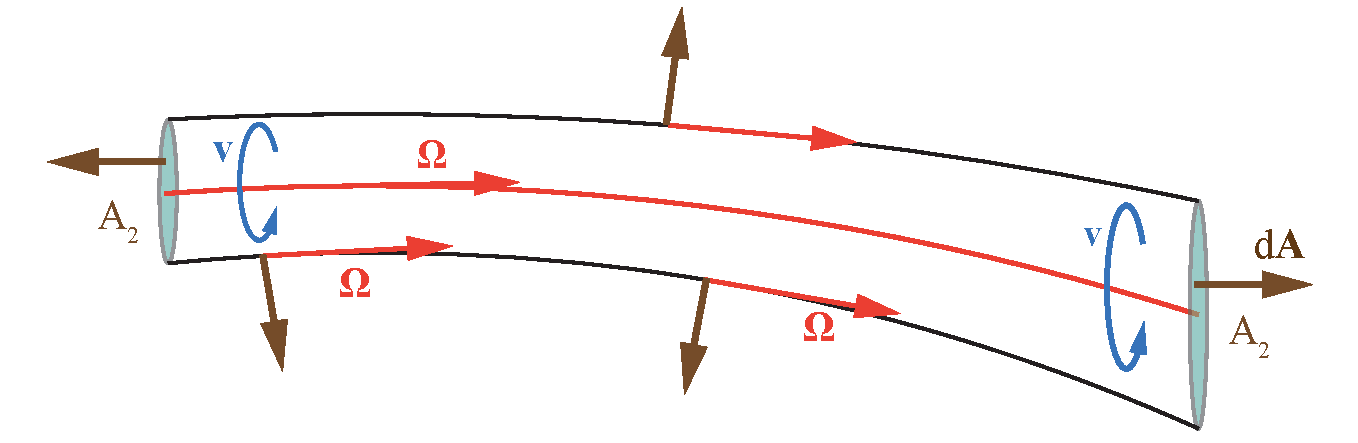
\includegraphics[width=\textwidth]{Wirbellinien}
  \caption[Veranschaulichung einer Wirbelr�hre]{Veranschaulichung einer
    Wirbelr�hre. Auf dem Mantel zeigt der Wirbelvektor parallel zur
    Oberfl�che. Er wird von Wirbellinien, die tangential an die Wirbelvektoren
    liegen, gebildet.}
    \label{abb:kontmech_Wirbelroehre}
\end{figure}


\subsection{Skalierungseigenschaften der Navier-Stokes-Gleichung}
\label{Skalierungseigenschaften!Navier-Stokes-Gleichung}

Wir haben gesehen, dass Str�mungen von vielen Faktoren abh�ngen. Oft untersucht
man jedoch technische Bauteile in Str�mungskan�len an verkleinerten Modellen.
Es ist m�glich, dabei zu Ergebnissen aus den Modellversuchen zu kommen, 
aus denen man direkt das Verhalten eines Systems bei realen Gr��enverh�ltnissen schlie�en kann.
Das liegt an den Skalierungseigenschaften der Navier-Stokes-Gleichung
\eqref{eq:kontmech_NavierStokesFrei}. Wir schreiben dazu die
Gleichung noch einmal auf,
\begin{equation*}
  \varrho \lk \lk \vec{v} \cdot \nablav \rk \vec{v} + \frac{\partial}
  {\partial t}\vec{v} \rk = \eta \, \Delta \vec{v} - \nablav p \; . \\
\end{equation*}
Um eine Skalierung der L�ngen durchf�hren zu k�nnen, f�hren wir eine
L�ngeneinheit $l$ so ein, dass wir in der Navier-Stokes-Gleichung nur
noch dimensionslose Ortsvariable stehen haben,
\begin{equation*}
  \vec{r} = l \, \tilde{\vec{r}} \, \qquad \nablav = \frac{1}{l} \tilde{\nablav}
  \; \quad \Delta = \frac{1}{l^2} \tilde{\Delta} \; .
\end{equation*}
Als weitere wichtige Gr��e geht die Str�mungsgeschwindigkeit ein. Auch f�r
diese f�hren wir mit der Geschwindigkeitseinheit $u$ �ber
\begin{equation*}
  \vec{v} = u \, \tilde{\vec{v}}
\end{equation*}
eine Skalierung ein. Aus diesen beiden folgt eine Zeiteinheit, die auch
auf Zeitableitungen anzuwenden ist,
\begin{equation*}
  t = \frac{l}{u} \, \tilde{t} \, \qquad \frac{\partial}{\partial t}
  = \frac{u}{l}\frac{\partial}{\partial \tilde{t}} \; .
\end{equation*}

Setzen wir alle diese Skalierungen ein, erhalten wir
\begin{equation*}
  \varrho \frac{u^2}{l} \lk \lk \tilde{\vec{v}} \cdot \tilde{\nablav} \rk
  \tilde{\vec{v}} + \frac{\partial}{\partial \tilde{t}} \tilde{\vec{v}} \rk
  = \frac{u}{l^2} \eta \, \tilde{\Delta} \tilde{\vec{v}} - \frac{1}{l}
  \tilde{\nablav} p \; , \\
\end{equation*}
was sich durch den Vorfaktor der linken Seite dividieren l�sst, sodass
wir
\begin{equation}
  \lk \tilde{\vec{v}} \cdot \tilde{\nablav} \rk \tilde{\vec{v}}
  + \frac{\partial}{\partial \tilde{t}} \tilde{\vec{v}} 
  = \frac{1}{u\,l\,\varrho} \eta \, \tilde{\Delta} \tilde{\vec{v}}
  - \tilde{\nablav} \frac{p}{\varrho\,u^2} \; \label{eq:kontmech_NavierStokesSkaliert01}
\end{equation}
erhalten.

Man erkennt also, dass man dasselbe Str�mungsverhalten erh�lt, wenn man die
\gls{reynoldszahl}\footnote{Osborne Reynolds (1842 -- 1912) war ein irisch-britischer Physiker. Nach ihm ist die Kennzahl zur Beurteilung viskoser Str�mungen und insbesondere deren �bergang zur Turbulenz benannt.}\indexp{Reynolds, Osborne}\index{Reynoldszahl}
\begin{equation}
  \mathrm{Re} = \frac{\varrho\,u\,l}{\eta}
\end{equation}
und den dimensionslosen Druck
\begin{equation}
  \tilde{p} = \frac{p}{\varrho\,u^2}
\end{equation}
konstant h�lt. In dieser Skalierung lautet die Navier-Stokes-Gleichung dann
\begin{equation}
  \lk \tilde{\vec{v}} \cdot \tilde{\nablav} \rk \tilde{\vec{v}}
  + \frac{\partial}{\partial \tilde{t}} \tilde{\vec{v}} 
  = \frac{1}{\mathrm{Re}} \, \tilde{\Delta} \tilde{\vec{v}}
  - \tilde{\nablav} \tilde{p} \; . \label{eq:kontmech_NavierStokesSkaliert02}
\end{equation}

�berschreitet die Reynolds-Zahl einen (problemabh�ngigen) kritischen Wert $\mathrm{Re}_\text{krit}$, wird eine bis dahin laminare Str�mung anf�llig gegen kleinste St�rungen und es findet ein �bergang von laminarer zu turbulenter Str�mung statt. F�r Experimente in der Hydrodynamik und Aerodynamik muss der Wert der Reynolds-Zahl von Original und verkleinerten Modell gleich sein, um ein �hnliches Str�mungsfeld zu erhalten. In der Literatur wird h�ufig ein Wert von $\mathrm{Re}_\text{krit} \approx 2300$ \cite{Schade1989, BergmannSchaefer1998} angegeben. 
Allerdings gibt die kritische Reynolds-Zahl nicht exakt den �bergang von einer laminaren zu einer turbulenten Str�mung an. H�ufig zerfallen Turbulenzen unterhalb der kritischen Reynolds-Zahl wieder schnell, insbesondere je kleiner die Reynolds-Zahl ist. Andererseits ist es in Experimenten gelungen, laminare Rohrstr�mungen mit Reynolds-Zahlen bis $\SI{50000}{}$ zu erzeugen, ohne dass dabei die Str�mung turbulent geworden ist \cite{Schade1989, BergmannSchaefer1998}. 




\clearpage
\section{Eigenschaften und Dynamik deformierbarer, fester K�rper}
\label{kap:kontmech_fest}\index{K�rper!elastische}\index{K�rper!deformierbare}

Bisher haben wir Fl�ssigkeiten und Gase als Beispiele f�r ein Kontinuum betrachtet. Doch wir ben�tigen auch
eine Beschreibung fester kontinuierlicher K�rper. Diese sind vor allem
durch ihr Verhalten bei Deformationen gekennzeichnet, das sich wesentlich von den Fluiden unterscheidet und das zur Beschreibung
ihrer Eigenschaften herangezogen wird. Diese Eigenschaften wollen wir zun�chst kl�ren,
bevor wir uns der Dynamik der Festk�rper-Kontinua widmen k�nnen.


\subsection{Eigenschaften deformierbarer K�rper}
\label{kap:kontmech_festEigenschaften}
\index{deformierbare K�rper!Eigenschaften}

Die Eigenschaften deformierbarer fester K�rper sind durch ihren (atomaren)
Aufbau gegeben. In einer einfachen klassischen Modellvorstellung k�nnen wir davon
ausgehen, dass alle Atomr�mpfe eines Festk�rpers sich so anordnen, dass
sich insgesamt und auch lokal ein energetisches (Potential-)Minimum ergibt. 
% im elektrostatischen Potential der Atome ein Minimum angenommen wird.
% Das elektrostatische Potentila ist ja bis hierher noch nicht eingef�ht.
Analog k�nnen wir in einer kontinuierlichen
Betrachtung modellieren, dass f�r eine bestimmte Konfiguration eines
materiellen Punkts des Kontinuums im Raum $\vec{r}_0$ ein Minimum des Potentials angenommen
wird. Wenn wir Deformationen betrachten, gehen wir von Abweichungen von
dieser idealen Lage der materiellen Punkte aus.

F�r kleine Abweichungen $\Delta \vec{r} = \vec{r} - \vec{r}_0$ entwickeln wir
das Potential in eine Potenzreihe um $\vec{r}_0$ (siehe auch \eqref{eq:bew_Schwingung_a} in \kap{bew_schwingung})
\begin{equation*}
  U(\vec{r}) = U(\vec{r}_0 + \D \vec{r}) = U(\vec{r}_0) + \nablav U(\vec{r}_0) \cdot \D \vec{r}
  + \frac{1}{2} \sum_{j,k}^3 \frac{\partial^2 U(\vec{r}_0)}{\partial x_j \,
    \partial x_k}\, \D x_j \, \D x_k + \dots \, ,
\end{equation*}
wobei oft nur die niedrigsten Ordnungen in Betracht gezogen werden m�ssen.
Die erste Ordnung verschwindet, da $\vec{r}_0$ ein Minimum darstellt,
wir erhalten also unter Benutzung der Einsteinschen Summenkonvention
\begin{equation*}
  U(\vec{r}) \approx \frac{1}{2} \, \frac{\partial^2 U(\vec{r}_0)}
  {\partial x_j \, \partial x_k}\, \D x_j \, \D x_k \; .
\end{equation*}
Das lineare Kraftgesetz ergibt sich in diesem Fall aus:
\begin{align}
  F_i(\vec{r}) &= \frac{1}{\d x_i} \, U(\vec{r}) \approx \frac{1}{2} \,
                  \frac{1}{\d x_i} \lek \frac{\partial^2 U(\vec{r}_0)} {\partial x_j \, \partial x_k}\, \stackrel{\downarrow}{\D x_j } \D x_k 
	                     +\frac{\partial^2 U(\vec{r}_0)} {\partial x_j \, \partial x_k}\,\D x_j \stackrel{\downarrow}{\D x_k }  \rek \notag \\
               &= \frac{1}{2} \lek \frac{\partial^2 U(\vec{r}_0)}{\partial x_j \,\partial x_k}\, \delta_{ij} \D x_k 
							                   + \frac{\partial^2 U(\vec{r}_0)}{\partial x_j \,\partial x_k}\, \delta_{ik} \D x_j \rek = \frac{\partial^2
  U(\vec{r}_0)} {\partial x_i \, \partial x_k}\, \Delta x_k \; . \label{eq:kontmech_kraefte_FK} 
\end{align}
Im Folgenden wollen wir verschiedene M�glichkeiten betrachten.

\subsubsection{Kontraktionen und Elastizit�tsmodul}
\label{kap:kontmech_festKontraktionen}
\index{Elastizit�tsmodul}

Als ersten Fall betrachten wir einen Festk�rper, der in eine Richtung
gedehnt wird und wollen die Kraftwirkung in genau diese Richtung wissen, siehe
\figref{kontmech_ElastTorsion}a. Wir interessieren uns also
f�r den Fall
\begin{equation}
  F_i = \frac{\partial^2 U(\vec{r}_0)}{\partial x_i \, \partial x_i}
  \, \Delta x_i \;,
  \label{eq:kontmech_Elastizitaetsmodul1}
\end{equation}
wobei wir von \eqref{eq:kontmech_kraefte_FK} zu \eqref{eq:kontmech_Elastizitaetsmodul1} zu kleinen Differenzgr��en $\Delta x_i $ �bergegangen sind. Dieser Fall tritt auf, wenn es keine Mischterme in den Ableitungen des Potentials
gibt. Es kann aber auch sein, dass ausschlie�lich $\Delta x_i \neq 0$.

\begin{figure}
  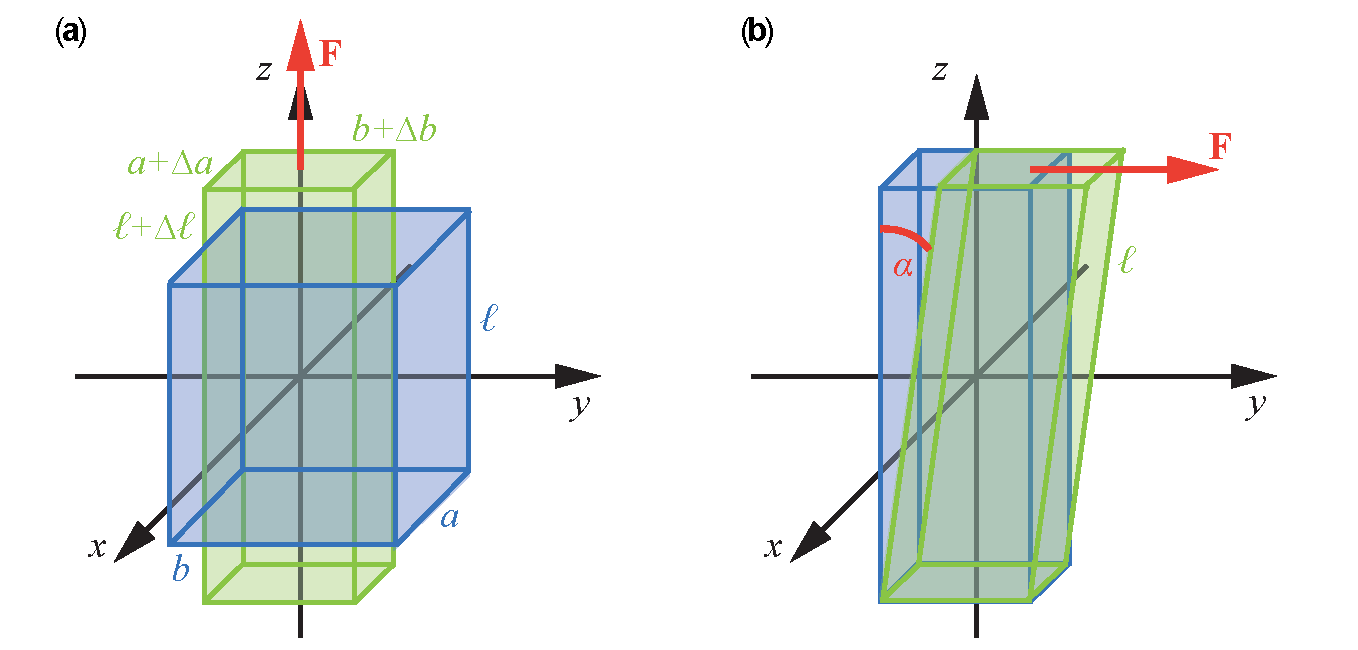
\includegraphics[width=\textwidth]{ElastTorsion.pdf}
  \caption[Zum Elastizit�tsmodul und Torsionsmodul]{Zum Elastizit�tsmodul und Torsionsmodul. \fa Darstellung einer
    Streckung mit der Zugkraft $\vec{F}$, die zur Definition des
    Elastizit�tsmoduls eingef�hrt wird. Dabei �ndern sich typischerweise auch
    die Ausdehnungen des K�rpers senkrecht zur Kraft. Die dazugeh�rigen
    Variablen $\Delta a$ und $\Delta b$ haben negative Werte. \fb Eine Scherung
    um den Winkel $\alpha$ f�hrt ebenfalls zu einem Widerstand, der durch die
    Kraft $\vec{F}$ �berwunden wird und �ber den sich das Torsionsmodul
    einf�hren l�sst.}
  \label{abb:kontmech_ElastTorsion}
\end{figure}

Mit dem Querschnitt $A$ des Elements des K�rpers, das verl�ngert wird, seiner
ungest�rten L�nge $\ell$ und der Verl�ngerung $\Delta \ell = \Delta x_i$
lasst sich Gleichung \eqref{eq:kontmech_Elastizitaetsmodul1} auf die Form
\begin{equation}
  F_i = \left ( \frac{\ell}{A} \frac{\partial^2 U(\vec{r}_0)}{\partial x_i
      \, \partial x_i} \right ) \, A \, \frac{\Delta \ell}{\ell}
  \label{eq:kontmech_Elastizitaetsmodul2}
\end{equation}
bringen. Mit dieser Form f�hrt man das \emph{\gls{Elastizitaetsmodul}}
\begin{equation}
  E = \frac{\ell}{A} \frac{\partial^2 U(\vec{r}_0)}{\partial x_i \,
    \partial x_i}
  \label{eq:kontmech_DefElastizitaetsmodul}
\end{equation}
ein und schreibt
\begin{equation}
  F = E \, A \, \frac{\Delta \ell}{\ell}
  \label{eq:kontmech_Elastizitaetsmodul3}
\end{equation}
beziehungsweise f�r die \emph{Zugspannung} $\sigma = F/A$
\begin{equation}
  \sigma = E \, \frac{\Delta \ell}{\ell} \; .
  \label{eq:kontmech_Elastizitaetsmodul4}
\end{equation}

�blicherweise �ndert sich jedoch nicht allein die L�nge des K�rpers. Es kommt
entlang der beiden Richtungen der Fl�che $A$ im Normalfall zu einer
Kontraktion. Um die Verk�rzung einer Richtung in der Fl�che zur Verl�ngerung
in der Richtung senkrecht dazu in Relation zu setzen (vgl.
\figref{kontmech_ElastTorsion}a), wird die \emph{\gls{Poissonzahl}}\footnote{Sim�on Denis Poisson (1781--1840 in Paris) war ein franz�sischer Physiker und Mathematiker. Er war Sch�ler von Laplace und besch�ftigte sich vor allem mit der Theorie der Wellen in der Akustik, der Elastizit�ts- und W�rmelehre, sowie �ber die Potentialtheorie der Elektrostatik. Als Mathematiker arbeitete Poisson vor allem auf den Gebietender Differentialgeometrie, der Infinitesimal- und Wahrscheinlichkeitsrechnung. Mehrere mathematische Begriffe sind mit seinem Namen verbunden. Er war sehr produktiv und ver�ffentlichte insgesamt �ber 300 Arbeiten.}\indexp{Poisson, Sim�on Denis}\index{Poissonzahl}
\begin{equation}
  \nu = -\frac{\Delta a\, /\, a}{\Delta \ell\, /\, \ell} =
  -\frac{\Delta b\, /\, b}{\Delta \ell\, /\, \ell}
  \label{eq:kontmech_Poissonzahl}
\end{equation}
eingef�hrt\footnote{Die Variablen $\Delta a$ und $\Delta b$, die die Stauchung
  in den beiden Richtungen senkrecht zur Streckung beschreiben, haben hier
  negative Werte. Die Poissonzahl ist so definiert, dass sie selbst positiv
  ist.}.
Typische Werte der Poissonzahl liegen f�r Metalle zwischen 0.2 und 0.4, f�r Beton bei 0.2 
und f�r Faserverbundstoffe bei kleiner 0.05.
Damit k�nnen wir nun die Deformation des gesamten Volumens betrachten. Diese
ergibt sich z.B. f�r eine rechteckige Fl�che zu
\begin{equation*}
  \Delta V = (a + \Delta a )(b + \Delta b )(\ell + \Delta \ell) - ab\ell \; ,
\end{equation*}
was f�r typischerweise kleine �nderungen in linearer N�herung zu
\begin{equation*}
  \Delta V = a b \Delta \ell + a \Delta b \ell + \Delta a b \ell
\end{equation*}
angegeben werden kann. F�r das Verh�ltnis findet man damit
\begin{equation*}
  \frac{\Delta V}{V} = \frac{\Delta \ell}{\ell} + \frac{\Delta a}{a} +
  \frac{\Delta b}{b} = \frac{\Delta \ell}{\ell} - \nu \frac{\Delta \ell}{\ell}
  -\nu \frac{\Delta \ell}{\ell}
  = ( 1 - 2 \nu )  \frac{\Delta \ell}{\ell} \; ,
\end{equation*}
was nun auch mit der angelegten Zugspannung verkn�pft werden kann,
\begin{equation*}
  \frac{\Delta V}{V} = \frac{\sigma}{E} ( 1 - 2 \nu ) \; .
\end{equation*}


\subsubsection{Inelastische K�rper}
\label{kap:kontmech_festinelastisch}
\index{deformierbare K�rper!inelastische}

Die bisherige Betrachtung ging davon aus, dass die Kraft allein durch die zweite
Ableitungen des Potentials ausgedr�ckt werden kann, also eine lineare Zunahme
der Kraft mit der Streckung oder Stauchung vorliegt. Dies ist der Fall
des Hookschen Gesetzes\index{Hooksches Gesetz|textbf}\indexp{Hooke, Robert}, das wir schon aus \kap{bew_newton_axioms}
kennen. Dies ist jedoch nicht beliebig der Fall, sondern gilt nur bis zur
\emph{Proportionalit�tsgrenze}\index{Proportionalit�tsgrenze!elastische K�rper}
im jeweiligen Material. Ist diese �berschritten, dehnt sich der K�rper bei
zunehmender Kraft st�rker aus, als es innerhalb der Proportionalit�tsgrenze
der Fall w�re.

Plastische Verformungen, die durch innere Umlagerungseffekte im Material
ausgel�st werden, treten bei noch h�heren Streckungen oder Kontraktionen auf.
Diese sorgen daf�r, dass das Material auch bei komplettem Verschwinden der
ausdehnenden Kraft nicht in seine urspr�ngliche Gestalt zur�ckkehrt.

Jedoch k�nnen auch innerhalb des Elastizit�tsbereichs zumindest kurzzeitige
Streckungen oder Stauchungen zur�ck bleiben, wenn keine Kraft mehr auf den
K�rper einwirkt. 
%Dies ist besonders bei sehr schnell einwirkenden Kr�ften der Fall.
In diesem Fall erh�lt man eine Hystereseschleife\index{Hysterese!elastische K�rper},
siehe \figref{kontmech_HystereseschleifeKompression}. Nach der Streckung des
K�rpers bis zum Punkt A durch die Zugspannung $\sigma_\text{A}$
und anschlie�ender Entspannung kehrt der K�rper nicht in den Ursprung zur�ck,
sondern es verbleibt eine restliche Streckung, die durch den Punkt C markiert
ist. Ein Druck bis zu $\sigma_\text{B}$ bewirkt eine Kompression bis zum
Punkt B. Entspannt man auch hier wieder bleibt die Stauchung, die durch den
Punkt D markiert ist, �brig.

\begin{figure}
  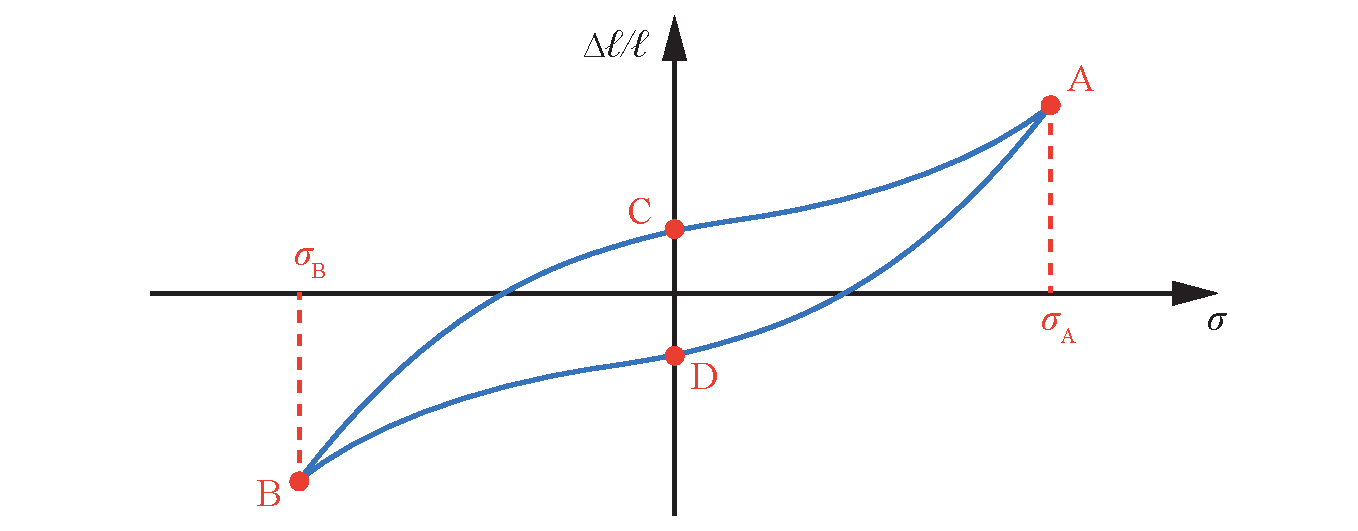
\includegraphics[width=\textwidth] {Spannungshysterese.pdf}
  \caption[Hystereseschleife\index{Hystereseschleife} bei Zugspannungen]{Mechanische
    Hystereseschleife bei der Kompression und Expansion eines elastischen
    K�rpers durch eine Zugspannung.}
  \label{abb:kontmech_HystereseschleifeKompression}
\end{figure}


\subsubsection{Scherungen und Torsionsmodul}
\label{kap:kontmech_festtorsion}
\index{Torsionsmodul|textbf}\index{Schubmodul|textbf}\index{Scherung}

Greift eine Kraft nicht senkrecht zur Fl�che eine K�rpers, sondern tangential
an, so f�hrt sie zu einer Scherung (siehe
\figref{kontmech_ElastTorsion}b). Der K�rper wird auch gegen diese
Bewegung einen Widerstand leisten, der durch eine Tangentialkraft $F_t$
�berwunden werden muss. Diese l�sst sich analog zu Gleichung
\eqref{eq:kontmech_Elastizitaetsmodul2} durch das innere Potential des
Festk�rpers ausdr�cken,
\begin{equation}
  F_t = \left ( \frac{1}{A} \frac{\partial^2 U(\vec{r}_0)}{\partial x_j
      \, \partial x_j} \frac{\partial \, (\Delta x_j)}{\partial \alpha} \right )
  \, A \, \alpha \; ,
  \label{eq:kontmech_Torsionsmodul1}
\end{equation}
wobei $\alpha$ der Winkel ist, um den die Scherung erfolgt. �hnlich
zum Elastizit�tsmoduls $E$ findet man f�r den Term in der Klammer
\begin{equation}
  G = \frac{1}{A} \frac{\partial^2 U(\vec{r}_0)}{\partial x_j
      \, \partial x_j} \frac{\partial (\Delta x_j)}{\partial \alpha} \; ,
  \label{eq:kontmech_Torsionsmodul2}
\end{equation}
der den Namen \emph{Torsionsmodul} oder \emph{\gls{Schubmodul}} erh�lt. �hnlich
der Zugspannung $\sigma$ l�sst sich unter Verwendung des Torsionsmoduls
die Scherspannung
\begin{equation}
  \tau = \frac{F_t}{A} = G \alpha
  \label{eq:kontmech_Torsionsmodul3}
\end{equation}
bilden.

F�r kleine Winkel kann man die Form von $G$ der von $E$ anpassen. Gehen wir davon
aus, dass $\alpha$ klein ist und somit $\sin \alpha \approx \alpha$ gilt, so
erhalten wir mit $\Delta x_j = \ell\, \sin \alpha \approx \ell\, \alpha$
\begin{equation*}
  \frac{\partial\, \Delta x_j}{\partial \alpha} = \frac{\partial \ell \alpha}
  {\partial \alpha} = \ell
\end{equation*}
und somit nimmt das Torsionsmodul die Gestalt
\begin{equation*}
  G = \frac{\ell}{A} \frac{\partial^2 U(\vec{r}_0)}{\partial x_j
    \, \partial x_j} 
\end{equation*}
an, die rein formal nicht mehr von der von $\ell$ zu unterscheiden ist. Ganz
analog findet man dann auch f�r die Tangentialkraft die zu
\eqref{eq:kontmech_Elastizitaetsmodul2} identische Form
\begin{equation}
  F_t = \lk \frac{\ell}{A} \frac{\partial^2 U(\vec{r}_0)}{\partial x_j
      \, \partial x_j} \rk \, A \, \frac{\Delta x_j}{\ell} \; .
  \label{eq:kontmech_Torsionsmodul4}
\end{equation}
Dabei muss man jedoch fest im Blick behalten, in welche Richtung die Kr�fte
angreifen. In der Komponentendarstellung, die wir gew�hlt haben, kommt nicht
zum Ausdruck, dass die Kraft tangential zur Fl�che angreift. Diese Tatsache
bildet jedoch den wesentlichen Unterschied zwischen Elastizit�ts- und Torsionsmodul.

\subsection{Dynamik deformierbarer K�rper}
\label{kap:kontmech_festDynamik}
\index{deformierbare K�rper!Dynamik}


\subsubsection{Lagrange-Formalismus f�r kontinuierliche K�rper}
\label{kap:kontmech_festLagrange}%
\index{Lagrange-Gleichung!kontinuierliche K�rper}%
%\index{schwingende Saite}
\index{Saite!schwingende|textbf}

Der Lagrange-Formalismus eignet sich gut, um dynamische Gleichungen auch f�r
elastische deformierbare K�rper aufzustellen. Um diesen motivieren zu k�nnen,
beginnen wir mit dem einfachen Beispiel einer schwingenden Saite. Diese
stellen wir uns zun�chst als eine Kette von Massepunkten identischer Masse $m$ vor,
die durch Federn der Ruhel�nge $d$ und der Federrichtgr��e $k_\text{F}$ miteinander
verbunden sind, siehe Abbildung \ref{abb:kontmech_SaiteMassepunkte}. Sp�ter
werden wir den Abstand $d$ zwischen den Massepunkten gegen Null gehen lassen,
um den �bergang zum kontinuierlichen System zu vollziehen.

\begin{figure}
  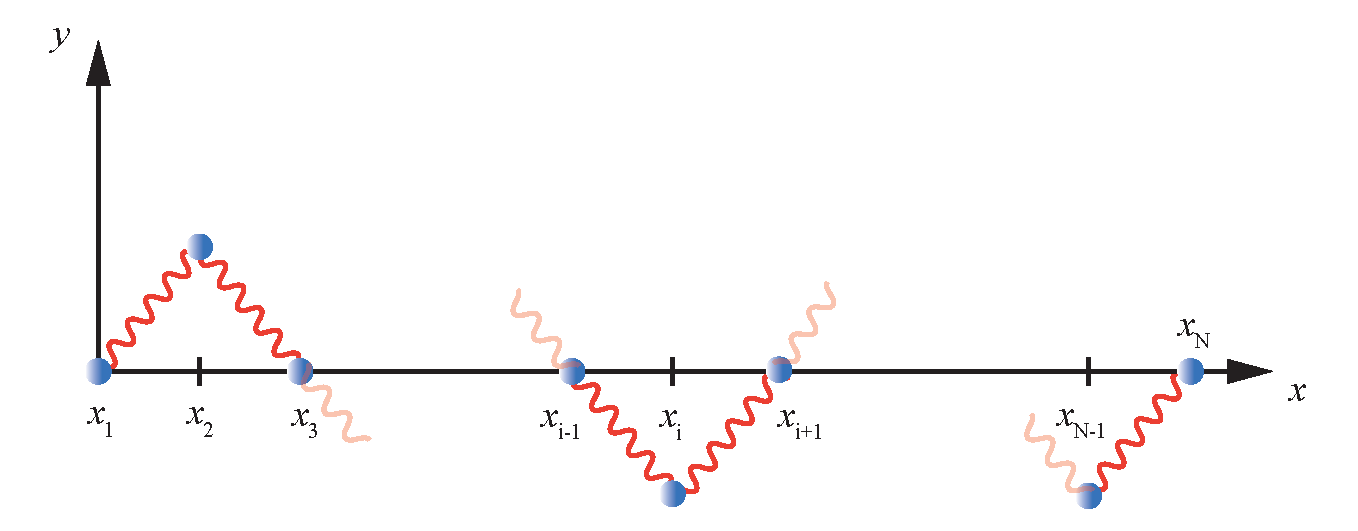
\includegraphics[width=\textwidth] {SchwingSaiteModell.pdf}
  \caption[Modell aus Massepunkten f�r eine schwingende Saite]{Eine schwingende
    Saite wird durch $N$ Massepunkte gleicher Masse $m_i=m$, die durch Federn verbunden
    sind, modelliert. Die Massen  $m_i$ f�r $i=0$ und $i=N-1$ sollen unbeweglich am
    Rand sein.}
    \label{abb:kontmech_SaiteMassepunkte}
\end{figure}

Entsprechend \kap{bew_Lagrange_II} m�ssen wir f�r die
Lagrange-Gleichungen zweiter Art zun�chst die kinetische Energie und das
Potential aufstellen. Das Modell setzt voraus, dass die Koordinaten $x_i$
fest bleiben und sich die Massepunkte nur in Richtung der $y_i$ bewegen k�nnen.
Damit ergibt sich f�r die kinetische Energie
\begin{equation*}
  T(\{\dot{y}_i\}) = \sum_{i=1}^N T_i = \sum_{i=1}^N \frac{m}{2} \,\dot{y}_i^2 \; .
\end{equation*}
F�r das Potential, das sich aus der angenommenen Feder zwischen den
Massepunkten $i-1$ und $i$ ergibt, gilt mit der Annahme, dass wir die
Abstands�nderungen in $x$-Richtung vernachl�ssigen k�nnen, weil diese Abst�nde als starr
angenommen werden und somit nicht zur Bewegung beitragen:
\begin{equation*}
  U(\{y_i\}) = \sum_{n=2}^{N} \frac{k_\text{F}}{2} (y_i - y_{i-1})^2 \; .
\end{equation*}
Somit l�sst sich die Lagrange-Funktion aufstellen zu
\begin{equation}
  \mathcal{L}(\{y_i\},\{\dot{y}_i\}) = T(\{\dot{y}_i\}) - U(\{y_i\})
  = \sum_{i=1}^N \frac{m}{2} \dot{y}_i^2
  - \sum_{i=2}^{N} \frac{k_\text{F}}{2} (y_i - y_{i-1})^2 \; .
  \label{kontmech_SaiteLagrangePunkte}
\end{equation}
Mit diesem Ansatz k�nnen wir zum kontinuierlichen System �bergehen. Dazu
verwenden wir die kontinuierliche Variable $x$ anstatt des Z�hlindex $i$
und schreiben f�r die Koordinaten
\begin{equation*}
  y_i \to y(x)\;, \qquad y_{i} - y_{i-1} \to \D x \, \left . \frac{\D y}{\D x} \right |_x  
\end{equation*}
und verwenden die (lineare) Dichte $\varrho_\mathrm{L}$ in $\SI{}{\kg\per\metre}$ statt der Masse $m$ sowie die Zugkraft\footnote{Diese entspricht hier in der eindimensionalen Betrachtung dem \gls{Elastizitaetsmodul} im mehrdimensionalen Fall.} $\Phi$ in $\SI{}{\N}$ statt der Federrichtgr��e $k_\text{F}$:
\begin{equation*}
  m = \varrho_\text{L} d \; , \qquad k_\text{F} = \frac{\Phi}{d} \; .
\end{equation*}
Dies f�hrt mit Gleichung \eqref{kontmech_SaiteLagrangePunkte} auf die
Lagrange-Funktion
\begin{align*}
  \mathcal{L} &= \sum_{i=1}^N \frac{\varrho_\text{L} d}{2} \lk \frac{\partial y(x,t)}
                {\partial t} \rk^2
                - \sum_{i=2}^{N} \frac{\Phi}{2 d} \lk \frac{\partial y(x,t)}
                {\partial x}
                \rk^2 d^2 \\
              &= \frac{\varrho d}{2} \left [
                \sum_{i=1}^N \lk \frac{\partial y(x,t)}{\partial t} \rk^2
                - \sum_{i=2}^{N} \frac{\Phi}{\varrho_\text{L}} \lk
                \frac{\partial y(x,t)}{\partial x} \rk^2 \right ] \; .
\end{align*}
Der Grenz�bergang zum kontinuierlichen System wird durch
\begin{equation*}
  d \sum_i \to \int \D x
\end{equation*}
vollzogen, was auf die kontinuierliche Lagrange-Funktion
\begin{equation}
   \mathcal{L} = \int \D x \; \frac{\varrho_\text{L}}{2} \left [
    \lk \frac{\partial y(x,t)}{\partial t} \rk^2 - \frac{\Phi}{\varrho_\text{L}}
    \lk \frac{\partial y(x,t)}{\partial x} \rk^2 \right ]
  \label{eq:kontmech_SaiteLagrangeFunktion}
\end{equation}
f�hrt.

In der Lagrange-Funktion \eqref{eq:kontmech_SaiteLagrangeFunktion} tritt die
\emph{Lagrange-Dichte}\index{Lagrange-Dichte|textbf}
\begin{equation}
  L \lk \frac{\partial y}{\partial t}, \frac{\partial y}{\partial x} \rk
  = \frac{\varrho_\text{L}}{2} \left [ \lk \frac{\partial y(x,t)}{\partial t} \rk^2
    - \frac{\Phi}{\varrho_\text{L}} \lk \frac{\partial y(x,t)}{\partial x} \rk^2
  \right ]
  \label{eq:kontmech_LagrangedichteSaite}
\end{equation}
auf, die wir heranziehen k�nnen, um die dynamischen Gleichungen zu gewinnen.

In \kap{bew_Lagrange_II} wurden die Lagrange-Gleichungen zweiter
Art aus denen erster Art durch den �bergang auf generalisierte Koordinaten
gewonnen. Man kann zeigen, dass sich dieselben Gleichungen aus einer
�quivalenten Forderung erhalten lassen. Die klassischen Bahnen sind n�mlich diejenigen, die
das \gls{Wirkungsfunktional}\index{Wirkungsfunktional}
\begin{equation*}
  S = \int \mathcal{L}(\{q_i\},\{\dot{q}_i\},t)\, \D t
\end{equation*}
extremal machen (siehe \cite{Schmutzer2005, Kuypers2012, Bartelmann2015}), f�r die also gilt
\begin{equation*}
  \delta S = \int \mathcal{L}(\{q_i+\delta q_i\},\{\dot{q}_i+\delta\dot{q}_i\}
  ,t)  \D t - \int \mathcal{L}(\{q_i\},\{\dot{q}_i\},t)\, \D t = 0  \; ,
\end{equation*}
wobei $\delta q_i(t)$ eine Variation der klassischen Bahn ist, die nur die
Randbedingung erf�llen muss, dass sie am Anfang und Ende der Bahn
verschwindet, also $\delta q_i(t_\mathrm{Start})=\delta q_i(t_\mathrm{Ende})=0$.
Dieselbe Forderung k�nnen wir an die Lagrange-Funktion\index{Lagrange-Funktion}
\eqref{eq:kontmech_SaiteLagrangeFunktion} der schwingenden Saite stellen. Dazu
f�hren wir die Variation der Auslenkung
\begin{equation*}
  y(x,t) = y(x,t) + \delta y(x,t)
\end{equation*}
ein und stellen das Wirkungsfunktional
\begin{equation}
  S = \int \mathcal{L}\,\D t = \int \D t \int \D x\,
  L \lk \frac{\partial y}{\partial t}, \frac{\partial y}{\partial x} \rk
\end{equation}
auf. Damit berechnen wir die Variation der Wirkung
\begin{align*}
  \delta S &= \int \D t \int \D x\,
             L \lk \frac{\partial y}{\partial t} + \frac{\partial \delta y}
             {\partial t},
             \frac{\partial y}{\partial x} + \frac{\partial \delta y}
             {\partial x}  \rk  - \int \D t \int \D x\,
             L \lk \frac{\partial y}{\partial t}, \frac{\partial y}
             {\partial x} \rk \; ,\\
  \intertext{was in linearer N�herung}
  \delta S &= \int \D t \int \D x\, \left [
             \frac{\partial L}{\partial \lk \frac{\partial y}{\partial t} \rk}
             \frac{\partial \delta y}{\partial t}
             + \frac{\partial L}{\partial \lk \frac{\partial y}{\partial x} \rk}
             \frac{\partial \delta y}{\partial x} \right ] \\
  \intertext{ergibt und mit partieller Integration auf}
  \delta S &= \int \D t \int \D x\, \left [
             -\frac{\partial}{\partial t} \frac{\partial L}
             {\partial \lk \frac{\partial y}{\partial t} \rk}
             - \frac{\partial}{\partial x} \frac{\partial L}
             {\partial \lk \frac{\partial y}{\partial x} \rk} \right ] \delta y
\end{align*}
f�hrt. Da die Variation $\delta y$ bis auf die Forderung nach verschwindenden Ver�nderungen an den Randpunkten
beliebig ist, fordert dies auch
\begin{equation}
  -\frac{\partial}{\partial t} \frac{\partial L}
  {\partial \lk \frac{\partial y}{\partial t} \rk}
  - \frac{\partial}{\partial x} \frac{\partial L}
  {\partial \lk \frac{\partial y}{\partial x} \rk} = 0
\end{equation}
und mit der Lagrange-Dichte\index{Lagrange-Dichte} der schwingenden Saite \eqref{eq:kontmech_LagrangedichteSaite}
erhalten wir schlie�lich:
\begin{equation}
  \varrho_\text{L} \frac{\partial^2 y(x,t)}{\partial t^2}
  - \Phi \frac{\partial^2 y(x,t)}{\partial x^2} = 0 \; .
  \label{eq:kontmech_PDGLSaite}
\end{equation}
Dies ist die gesuchte dynamische Gleichung f�r die schwingende Saite. Dividiert man beide Seiten von \eqref{eq:kontmech_PDGLSaite} durch die als konstant angenommene Querschnittsfl�che $A$, dann erh�lt man mit dem \gls{Elastizitaetsmodul} $E = \Phi / A$ die \emph{Wellengleichung}\index{Wellengleichung} f�r die schwingende Saite in der �blichen Darstellung mit der Volumendichte $\varrho$:
\begin{equation}
  \varrho \frac{\partial^2 y(x,t)}{\partial t^2}
  - E \frac{\partial^2 y(x,t)}{\partial x^2} = 0 \; .
  \label{eq:kontmech_PDGLSaite2}
\end{equation}


\newpage
%BEISPIEL %%%%%%%%%%%%%%%%%%%%%%%%%%%%%%%%%%%%%%%%%%%%%%%%%%%%%%%%%%%%%%%%%%%%%%%%%%%%%%%%%%
\begin{example}{Analytische L�sungen f�r die schwingende Saite}
\label{bsp:kontmech_schwingendeSaite}\index{Saite!schwingende}
\smallskip

Die Wellengleichung \eqref{eq:kontmech_PDGLSaite2} hat sehr
viele verschiedene L�sungen, die meist durch Randbedingungen eingeschr�nkt
sind. Wir wollen uns hier auf zwei L�sungstypen beschr�nken.

Zun�chst betrachten wir L�sungen, die wir mit dem Produktansatz
\begin{equation*}
  y(t,x) = a(t)\,b(x) 
\end{equation*}
finden. Setzt man diesen in \eqref{eq:kontmech_PDGLSaite2} ein, k�nnen wir
dies auf die Form
\begin{equation*}
  \frac{1}{a(t)} \frac{\partial^2 a(t)}{\partial t^2} = \frac{E}{\varrho}
  \frac{1}{b(x)} \frac{\partial^2 b(x)}{\partial x^2} = C
\end{equation*}
bringen, wobei $C$ eine Konstante sein muss, da eine Seite nur von $t$, die
andere nur von $y$ abh�ngt. Dies erm�glicht uns, die beiden separierten
Differentialgleichungen getrennt zu l�sen. So finden wir \zb sehr einfach
die L�sungen
\begin{align*}
  a(t) &= \alpha_1 \mathrm{e}^{\sqrt{C}t} + \alpha_2 \mathrm{e}^{-\sqrt{C}t}
         \; , \\
  b(x) &= \beta_1 \mathrm{e}^{\sqrt{\frac{\varrho}{E} C}x}
         + \beta_2 \mathrm{e}^{-\sqrt{\frac{\varrho}{E} C}x} \; .
\end{align*}
Interessant f�r das Verhalten einer schwingenden Saite sind dabei vor allem
L�sungen, die nicht exponentiell anwachsen. Diese erhalten wir f�r ein negatives
$C$ und wir setzen nun
\begin{equation*}
  \sqrt{C} = \im \omega \; , \qquad \sqrt{\frac{\varrho}{E} C} = \im k
  \; ,
\end{equation*}
womit wir 
\begin{align*}
  a(t) &= \alpha_1 \mathrm{e}^{\im \omega t} + \alpha_2
         \mathrm{e}^{-\im \omega t} \; , \\
  b(x) &= \beta_1 \mathrm{e}^{\im k x} + \beta_2 \mathrm{e}^{-\im k x} 
\end{align*}
beziehungsweise
\begin{equation*}
  y(t,x) = \left \{ \alpha_1 \mathrm{e}^{\im \omega t} + \alpha_2
    \mathrm{e}^{-\im \omega t} \right \} \left \{ \beta_1 \mathrm{e}^{\im k x}
    + \beta_2 \mathrm{e}^{-\im k x}  \right \}
\end{equation*}
erhalten. Dies sind stehende Wellen, bei denen periodische r�umliche Strukturen
unabh�ngig vom Zeitverlauf bestehen. Der Zeitverlauf �ndert allein die Gr��e
Auslenkungen, nicht aber ihre Position entlang der Saite. Leichter sichtbar wird das f�r den Spezialfall $\alpha_1 = \alpha_2
= \alpha/2$, $\beta_1 = \beta_2 = \beta/2$, was auf die L�sung
\begin{equation*}
  y(t,x) = \alpha \beta \cos(\omega t) \cos(k x) 
\end{equation*}
f�hrt. Graphische Darstellungen finden sich in Beispiel
\ref{bsp:kontmech_finiteDiffSaite}, in dem wir dieses System numerisch mit der
Methode der finiten Differenzen l�sen werden.

Einen zweiten Typ von L�sungen, den wir betrachten wollen, sind fortlaufende
Wellen, die eine nahezu beliebige funktionale Form haben d�rfen. Der
Ansatz
\begin{equation*}
  y(t,x) = f(\omega t \pm kx)
\end{equation*}
mit $k$ als Wellenzahl und $\omega$ als Kreisfrequenz l�st ganz allgemein, wie man durch Einsetzen erkennt,
\begin{equation*}
  \varrho \omega^2 f''(\omega t \pm kx) = E k^2 f''(\omega t \pm kx) \; ,
\end{equation*}
die Differentialgleichung, falls die \gls{Dispersionsrelation} \index{Dispersionsrelation} 
\begin{equation}
  \omega = \sqrt{\frac{E}{\varrho}}\,k
  \label{eq:kontmech_DispersionsRel}
\end{equation}
erf�llt ist. F�r eine beidseitig eingespannte Saite verbieten sich jedoch solche L�sungen wegen der Randbedingungen.
Da die
Differentialgleichung linear ist, sind jederzeit beliebige �berlagerungen von L�sungen der beidseitig eingespannte Saite m�glich,
die in der Summe sich als ausbreitende Wellen auf der Saite interpretieren lassen. Beispiele werden
wir in \probref{kontmech_WelleSaite} untersuchen.
\end{example}

%BEISPIEL %%%%%%%%%%%%%%%%%%%%%%%%%%%%%%%%%%%%%%%%%%%%%%%%%%%%%%%%%%%%%%%%%%%%%%%%%%%%%%%%%%


\subsubsection{Numerisches L�sungsverfahren �ber finite Differenzen}
\label{kap:kontemch_finiteDifferenzen}
\index{Finite Differenzen Methode}\index{Differenzen!finite}\index{Finite Differenzen Methode|textbf}

Lineare \emph{\gls{PDGL}en}\index{Differentialgleichung!partielle} (PDGL) der Form
\begin{equation}
  \left ( \sum_i a_i \frac{\partial^2}{\partial x_i^2} +
    \sum_i b_i \frac{\partial}{\partial x_i} + c \right )
  f(\vec{x}) + d = 0 \; ,   \label{eq:kontmech_GrundformPDGL1}
\end{equation}
zu denen auch die Differentialgleichung \eqref{eq:kontmech_PDGLSaite} der
schwingenden Saite geh�rt, lassen sich numerisch mit finiten Differenzen
l�sen. Wir k�nnen das hier nicht vollst�ndig einf�hren, wollen aber kurz die
Idee der L�sungsmethode vermitteln und verweisen auf das entsprechende Kapitel
im L�sungsteil \bzw auf die Literatur \cite{Otto2019, Fischer2014, Riley2006,
  Andrews2003}.
Wir beschr�nken uns auf den Fall einer PDGL 2. Ordnung mit zwei Variablen
($x_1 =x\,,\,\,x_2=t$), so dass aus \eqref{eq:kontmech_GrundformPDGL1} 
\begin{align}
  \lk a_{11} \frac{\partial^2}{\partial x^2} + a_{12} \frac{\partial^2}{\partial x\,\partial t} + a_{21} \frac{\partial^2}{\partial t\,\partial x } + a_{22} \frac{\partial^2}{\partial t^2} 
   + b_1 \frac{\partial}{\partial x} + b_2 \frac{\partial}{\partial t} + c \rk \,f(x,t)\nonumber \\
	&~~+ d = 0    \label{eq:kontmech_GrundformPDGL2}
\end{align}
wird.\\
Definiert man die Diskriminante
	\[\mathcal{D} = a_{11}\,a_{22} - \frac{a_{12}\,a_{21}}{4} \,,\]
dann unterscheidet man bei \eqref{eq:kontmech_GrundformPDGL2} verschiedene Typen:
Gilt $\mathcal{D}(x,t) > 0$, so hei�t die PDGL elliptisch im Punkt $(x,t)$, 
f�r $\mathcal{D}(x,t) = 0$ ist die PDGL parabolisch im Punkt $(x,t)$, 
und gilt $\mathcal{D}(x,t) <0$, so haben wir im Punkt $(x,t)$ eine hyperbolische PDGL vorliegen\footnote{Der Ursprung der Bezeichnungen elliptisch, parabolisch und hyperbolisch ergibt sich aus der Theorie der Kegelschnitte. Die allgemeine Kegelschnittgleichung $a_{11}\,x^{2}+a_{12}\,x\,y+a_{22}\,y^{2}+b_1\,x+b_2\,y+c=0$ 
ist von der Struktur her �hnlich aufgebaut wie die lineare partielle Differentialgleichung 2. Ordnung \eqref{eq:kontmech_GrundformPDGL2}.}.
Man findet unterschiedliche L�sungsprogramme f�r die einzelnen Typen. 
Die Wellengleichung als dynamische Gleichung f�r die schwingende Saite ist offensichtlich vom hyperbolischen Typus, denn es gilt $\mathcal{D}(x,t) = -\varrho E <0$.

Die L�sungsmethode der finiten Differenzen f�r diesen Fall baut nun darauf auf, dass man
die gesuchte Funktion $f(x,t)$ auf Gitterpunkten
\begin{equation*}
  (x = x_i \,, t = t_l)
\end{equation*}
definiert und damit das Differentialgleichungssystem diskretisiert. Man
bestimmt in der L�sung also die Daten $f(x_i,t_l)$ f�r alle
Indexkombinationen.

Dazu m�ssen nat�rlich auch die Ableitungen diskretisiert werden. Dies gelingt
zum Beispiel f�r ein (eindimensionales) Gitter aus �quidistanten Schritten $x_i = x_0 + i\,$
durch
\begin{subequations}
  \begin{align}
    \frac{\partial f(x_i)}{\partial x_i} &= \frac{f(x_{i+1}) - f(x_{i-1})}
                                           {2\Delta x}  \; ,
    \label{eq:kontmech_Diskretisierung1} \\
    \frac{\partial^2 f(x_i)}{\partial x_i^2} &= \frac{f(x_{i+1}) + f(x_{i-1})
                                               -2 f(x_i)}{\Delta x^2}
    \label{eq:kontmech_Diskretisierung2} \; ,
\end{align}
\end{subequations}
was nat�rlich analog f�r alle anderen Variablen gilt, w�hrend diese f�r
die $x$-Ableitungen festgehalten werden. Hier muss man nur
bedenken, dass die Randpunkte gesondert behandelt werden m�ssen, da die
Ableitungen symmetrisch aufgebaut sind. Bei unserer PDGL haben wir sogenannte 
Dirichlet\footnote{Dirichlet (1805�-1859) war ein deutscher Mathematiker, der haupts�chlich auf den Gebieten der Analysis und der Zahlentheorie t�tig war.}\indexp{Dirichlet, Peter Gustav Lejeune}-Randbedingungen\index{Randbedingungen!Dirichletsche}\footnote{Die Dirichlet-Randbedingung ist in der Mathematik eine Randbedingung, bei der die Ableitungen einer L�sung nur innerhalb der Dom�nengrenze angewendet wird.} vorliegen, die wir dadurch definieren, dass die Randwerte, \zb
$x_0,\, t_0$ und $x_{N+1},\, t_{N+1}$, auf einen festen Wert gesetzt werden,
\dh die Randpunkte werden im L�sungsverfahren nicht ge�ndert.

Prinzipiell kann man damit das Differentialgleichungssystem auf die 
Form einer Matrixgleichung f�r ein lineares Gleichungssystem
\begin{equation*}
  \mathbb{M} \,\vec{f} = \vec{0}
\end{equation*}
bringen (siehe auch \cite{Fischer2014}). Man sucht also f�r dieses lineare
Gleichungssystem den L�sungsvektor $\vec{f}$. Dieses Verfahren wird jedoch in
seiner Allgemeinheit relativ selten verwendet, da es sehr aufwendig ist.

In der Physik versucht man meist zu bestimmen, wie sich eine Bewegung K�rpers/Objektes
wie der schwingenden Saite in der Zeit ver�ndert. In diesem Fall
stellt man eine Iterationsgleichung f�r die Zeitschritte auf. Wie das
funktioniert, l�sst sich am einfachsten an einem Beispiel erkl�ren. Daf�r
greifen wir wieder auf die schwingende Saite zur�ck.

% BEISPIEL %%%%%%%%%%%%%%%%%%%%%%%%%%%%%%%%%%%%%%%%%%%%%%%%%%%%%%%%%%%%%%%%%%%%%%%%%%%%%%%%%%
\begin{example}{Numerische L�sungen zur schwingenden Saite}
\label{bsp:kontmech_finiteDiffSaite}\index{Saite!schwingende}
\smallskip
In der Differentialgleichung \eqref{eq:kontmech_PDGLSaite2} der schwingenden
Saite treten sowohl in $x$ als auch in $t$ ausschlie�lich zweite Ableitungen
auf. Mit dem Diskretisierungsansatz \eqref{eq:kontmech_Diskretisierung2},
stellen wir also die diskreten Terme
\begin{equation*}
  \frac{y(x_i,t_{l+1}) + y(x_i,t_{l-1}) -2 y(x_{i},t_{l})}{\Delta t^2}
  = \frac{\kappa}{\varrho} \frac{y(x_{i+1},t_l) + y(x_{i-1},t_l)-2 y(x_i,t_l)}
  {\Delta x^2}
\end{equation*}
auf. Dies l�sen wir nach $y(x_i,t_{l+1})$ auf, um die Entwicklung in
der Zeit iterativ zu berechnen. Man erh�lt
\begin{align}
\begin{split}
  y(x_i,t_{l+1}) = 2 y(x_{i},t_{l}) - y(x_i,t_{l-1}) \\
	&~~~+ \frac{\kappa}{\varrho}
  \frac{\Delta t^2}{\Delta x^2} \left ( y(x_{i+1},t_l) + y(x_{i-1},t_l)
    -2 y(x_i,t_l) \right ) \; .
\end{split} \label{eq:kontmech_bsp6}
\end{align}
Kennt man das volle Raumgitter also f�r die zwei vorherigen Zeitschritte,
l�sst sich die L�sung der partiellen Differentialgleichung auf diese Weise f�r
alle weiteren bestimmen.
Im \mscr~ \mlkontmechref{SchwingendeSaite01.m} findet sich ein Programm, das diese
L�sung umsetzt. Eine Schwingung wird f�r eine Saite der L�nge $L =
\SI{10}{\centi\metre}$ sowie die Materialparameter $\varrho = \SI{1150}
{\kilo\gram\per \metre^3}$ und $\kappa = \SI{3e9}{\pascal}$ (typisch f�r Darm- \bzw Nylonsaiten) berechnet. Zu Beginn wird
eine Welle angenommen, die die Randbedingungen $y(x=0,t) = y(x=L,t) = 0$
erf�llt. Sie wird f�r die ersten beiden Zeitschritte identisch eingesetzt,
um eine maximale Auslenkung zu implementieren. In
\figref{kontmech_SaiteStehendeWelle} ist das Ergebnis f�r mehrere
Zeitschritte dargestellt. Das typische Verhalten einer stehenden Welle
ist gut zu erkennen.

\begin{center}
  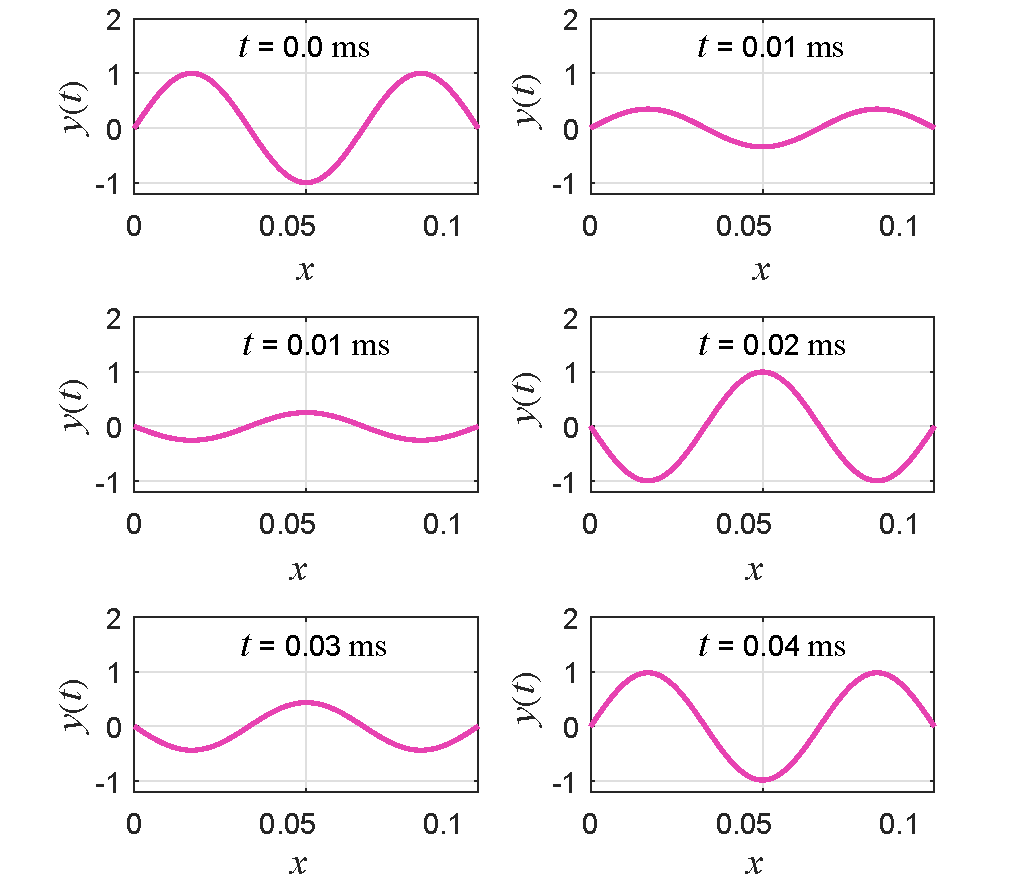
\includegraphics[width=\textwidth]{SchwingendeSaite01.pdf}
  \captionof{figure}{Stehende Welle\index{Welle!stehende} auf einer Saite. Siehe \mscr~ \mlkontmechref{SchwingendeSaite01.m}.}\label{abb:kontmech_SaiteStehendeWelle}
\end{center}

Selbstverst�ndlich k�nnen aber auch laufende Wellen\index{Welle!laufende}, f�r die analytische
L�sungen deutlich schwieriger zu finden sind mit dieser numerischen Methode
behandelt werden. Dies wollen wir in \probref{kontmech_WelleSaite}
tun.
\end{example}
% BEISPIEL %%%%%%%%%%%%%%%%%%%%%%%%%%%%%%%%%%%%%%%%%%%%%%%%%%%%%%%%%%%%%%%%%%%%%%%%%%%%%%%%%%

Geht man zu zwei Dimensionen �ber und betrachtet Schwingungen einer Ebene,
lassen sich die \emph{Chladnischen}\footnote{Ernst Florens Friedrich Chladni (1756--1827) war ein deutscher Physiker und Astronom. Er beschrieb die nach ihm benannten Klangfiguren und erkl�rte die Herkunft von Meteoriten.}\indexp{Chladni, Ernst Florens Friedrich} \emph{Klangfiguren} finden. Die zugeh�rige partielle
Differentialgleichung wird in \probref{kontmech_Chladni} gel�st.

Der gefundene kontinuierlichen Ansatz f�r die schwingende Saite l�sst sich
leicht erweitern. Ganz �hnlich l�sst sich z.B. das Problem der Achterbahn, die
in \probref{bew_achterbahn_diskret} durch diskrete Wagen simuliert wurde,
wieder aufgreifen, indem man den Grenzwert eines kontinierlichen Zuges bildet.
Auf diese Weise kann man sich dem kontinuierlichen Modell aus 
\kap{rollercoaster} ann�hern, ohne dabei die N�herung eines vollkommen
starren Zuges einf�hren zu m�ssen. Die Herleitung des Kontinuums-Grenzwerts
wird in \probref{kontmech_AchterbahnKont} durchgef�hrt,
\probref{kontmech_AchterbahnZug} widmet sich dann einer numerischen L�sung
und Betrachtungen f�r die Normalbeschleunigung erfolgen in
\probref{kontmech_AchterbahnBeschleunigungen}.


\subsubsection{Ausblick: Dynamik elastischer K�rper}
\label{kap:kontmech_festelastisch}
\index{K�rper!Dynamik elastischer}\index{K�rper!elastische}

Die Dynamik elastischer K�rper ist \iA sehr komplex. Dies hat
sich schon in \kap{kontmech_festEigenschaften} angedeutet,
da z.B. die Verl�ngerung eines K�rpers in der Regel auch eine Verk�rzung
in den Richtungen senkrecht dazu zur Folge hat. F�r eine vollst�ndige
Behandlung muss man alle Richtungen zusammen betrachten.
Ein solch umfangreicher Ansatz geht �ber den Umfang dieses Buches hinaus, wir verweisen auf die weiterf�hrende
Literatur, z.B. \cite{Altenbach1994,Altenbach2018,Rannacher2017}. Wir wollen hier aber angeben, welche Bewegungsgleichungen in der Dynamik elastischer K�rper gel�st werden m�ssen und
wie diese zu verstehen sind.

Als unabh�ngige Koordinaten f�r eine Ausgangskonfiguration bieten sich f�r
eine Betrachtung elastischer K�rper die materiellen Punkte $\vec{\hat{P}}$  nach der
Definition aus Gleichung \eqref{eq:kontmech_Materiepunkt} an. Wir w�hlen
jedoch die Materiepunkte nicht zu einem beliebigen Zeitpunkt $t_0$, sondern
so, dass sich alle Materiepunkte in einer Gleichgewichtslage befinden. In
dieser Gleichgewichtslage gilt also
\begin{equation*}
  \vec{r}_0 = \vec{\hat{P}}_0  \; .
\end{equation*}
Wir interessieren uns f�r die Auslenkungen eines Materiepunktes aus der Ruhelage, die wir mit $\vec{u}$ wollen:
\begin{equation*}
  \vec{u}(\vec{\hat{P}}) = \vec{r}(\vec{\vec{\hat{P}}}) - \vec{r}_{0}(\vec{\hat{P}})
  = \vec{r}(\vec{\hat{P}}) - \vec{\hat{P}}_0 \,.
\end{equation*}
Es ist zu erwarten, dass in einem
K�rper, der unter Spannung steht, diese Auslenkung f�r jeden Materiepunkt
verschieden ist\footnote{W�re sie f�r alle Punkte gleich, w�re dies nur
  eine Verschiebung des ganzen, unver�nderten K�rpers, was f�r die
  Betrachtung der inneren Dynamik uninteressant w�re.}. Alle m�glichen
Deformationen stellen wir durch die Ableitungen
\begin{equation}
  \frac{\partial r_i(\vec{\hat{P}})}{\partial r_j}
\end{equation}
dar. Sie enthalten Deformationen sowohl in L�ngs- als auch Querrichtung und
k�nnen prinzipiell als Elemente einer Matrix geschrieben werden.

Vollkommen analog betrachten wir die Spannungen im K�rper in allen m�glichen
Richtungen durch das Einf�hren des \emph{Spannungstensors}\index{Spannungstensor|textbf}
$\hat{\vec{\sigma}}$. Seine Diagonalelemente enthalten die Zug- und Druckspannungen,
w�hrend Scherspannungen in den Nichtdiagonalelementen notiert werden. Gehen wir
von einem Material aus, in dem die Deformationen linear von den Spannungen
abh�ngen, l�sst sich das verallgemeinerte Hooksche\indexp{Hooke, Robert}
Gesetz\index{Hooksches Gesetz}
\begin{equation}
    \hat{\vec{\sigma}} = \mathbb{C}\, \hat{\vec{\epsilon}} \quad \text{\bzw} \quad  \hat{\sigma}_{ij} = C_{ijkl} \,\hat{\epsilon}_{kl} 
\end{equation}
finden, wobei wir bei der Komponentenschreibweise die Einsteinschen Summenkonvention verwendet haben.
Im Spannungstensor $\hat{\vec{\sigma}}$ kommt der lineare und symmetrische
\emph{Verzerrungstensor}\index{Verzerrungstensor} $\hat{\vec{\epsilon}}$ vor:
\begin{align}
    \hat{\vec{\epsilon}} &= \frac{1}{2} \lk \nablav \vec{u} + \lk \nablav
    \vec{u} \rk^T \rk \quad \text{\bzw} \quad  \hat{\epsilon}_{kl} = \frac{1}{2} \lk \frac{\partial u_k}{\partial p_l} +
                 \frac{\partial u_l}{\partial p_k}  \rk \,.
\end{align}
Offensichtlich ist $\mathbb{C}$ ein Tensor vierter Stufe, der vier
Indizes besitzt. Ist das Material dar�ber hinaus isotrop, vereinfacht
sich der Zusammenhang und es ergeben sich die Beziehungen
\begin{subequations}
  \begin{align}
    \hat{\vec{\sigma}} &= 2 \mu \hat{\vec{\epsilon}} + \lambda \, \mathrm{Sp}(
                   \,\hat{\vec{\epsilon}}) \, \mathbb{I} \; , \\
    \hat{\vec{\sigma}} &= \mu \lk \nablav \vec{u} +  \lk \nablav \vec{u} \rk^T \rk
                   + \lambda \lk \nablav
                   \cdot \vec{u} \rk \,\mathbb{I}  \; , \\
    \hat{\sigma}_{ij} &= \mu \lk  \frac{\partial u_i}{\partial p_j} +
                  \frac{\partial u_j}{\partial p_i} \rk + \lambda
                  \,\frac{\partial u_k}{\partial p_k} \delta_{ij}
                  \label{eq:kontmech_Spannungstensor1}
  \end{align}
\end{subequations}
  mit der Einheitsmatrix $\mathbb{I}$. $\mathrm{Sp}(\hat{\vec{\epsilon}})$ ist die Spur des Tensors $\hat{\vec{\epsilon}}$ und die sogenannten \emph{Lam\'e}\footnote{Gabriel Lam\'e (1795--1870) war ein franz�sischer Mathematiker und Physiker, der 
auf dem Gebiet der Differentialgeometrie und der mathematischen Physik arbeitete. Er wurde ber�hmt f�r seine allgemeine L�sung der W�rmeleitungsgleichung.}\indexp{Lam\'e, Gabriel}-\emph{Konstanten}\index{Lam\'e-Konstanten} sind gegeben durch
\begin{subequations}
  \begin{align}
    \lambda &= \frac{\nu}{(1-2\nu)(1+\nu)} E \; ,\\
    \mu &= G = \frac{1}{2} \frac{1}{1+\nu} E \; ,
  \end{align}
\end{subequations}
wobei die zweite Lam\'e-Konstante $\mu$ dem bereits eingef�hrten Torsions-
oder \gls{Schubmodul}\index{Torsionsmodul}\index{Schubmodul} $G$ aus den
Gleichungen \eqref{eq:kontmech_Torsionsmodul1} bzw.
\eqref{eq:kontmech_Torsionsmodul3} entspricht und $\lambda$ offensichtlich in enger Beziehung zum Elastizit�tsmodul $E$ steht.

Dass die eingef�hrten Elastizit�ts- und Torsionsmodule aus den Kapiteln
\ref{kap:kontmech_festKontraktionen} und \ref{kap:kontmech_festtorsion}
die richtigen Spezialf�lle darstellen, die im dreidimensionalen
Spannungstensor enthalten sind, wird in \probref{kontmech_ElastizitaetTorsion}
herausgearbeitet. Als eine wichtige Anwendung von Spannungen in K�rpern wird
in \probref{kontmech_BogenSpannung} die Spannung eines Bogens durch eine
Saite untersucht.
  
Bleiben in der Dynamik alle Beziehungen linear, lautet die Bewegungsgleichung
f�r die Verzerrungen $\vec{u}$
  \begin{align}
    \varrho \,\frac{\partial^2 \vec{u}}{\partial t^2}
    &= \nabla \cdot \hat{\vec{\sigma}} + \varrho \,\vec{f} \quad \text{\bzw} \quad
    \varrho \,\frac{\partial^2 u_i}{\partial t^2}
    = \sum_j \frac{\partial \hat{\sigma}_{ji}}{\partial p_j} + \varrho\, f_i \; ,
  \end{align}
wobei $\vec{f}$ eine auf ein Volumenelement angreifende Kraftdichte in $\SI{}{\newton\per\metre\cubed}$ und
$\varrho$ die Massendichte ist.

%\clearpage
%\section{Tabellen}\label{kap:km_tabellen}

\clearpage



\clearpage
\input{kontmech/kontmech_uebungen} 
%\clearpage
%\section{L�sungsbeispiele Kapitel \ref{chap:kontmech} -- Physik des Kontinuums}\label{chap:kontmech_lsguebungen}

Die in den L�sungsvorschl�gen angegebenen \mscre finden sich im GitHub unter \githubSN \bzw
in den \onlineZ{} (\MKc).\\
Sie sind wirklich als Vorschlag f�r eine m�gliche L�sung gedacht, wohl wissend, dass es in der Physik oft ganz verschiedene, manchmal auch elegantere als die hier vorgestellten L�sungen gibt, um ein Problem zu l�sen. Das macht ja gerade den Reiz der Physik aus.
Wir laden die Leser ein, ihre L�sungen auch unter \githubSN \bzw auf den online-Seiten (\MKc) zu teilen.
Wir sind in jedem Fall gespannt.

%-----------------------------------------------------------------------------------------------------------

\subsection{�bungen zu Bewegungen von Fl�ssigkeiten und Gasen}

\medskip

%-----------------------------------------------------------------------------------------------------------

\begin{sol}{prob:kontmech_diffoperators}\label{lsg:kontmech_diffoperators} %�bung1
\textbf{Differentialoperatoren}
\begin{enumerate}
    \item [1.]
    \begin{enumerate}
        \item [a)]
        \begin{align}
            \Phi \lk \vec{r}\rk &= x\,y\,\e^{-r^2} ~~\rightarrow~~~ \gradv\,\Phi = \begin{pmatrix}
                y-2x^2\,y\\
                x-2x\,y^2\\
                -x\,y\,z
            \end{pmatrix}\,
            \e^{-r^2} \,. \label{eq:kontmech_Ueb1_01}
        \end{align}
        \item[b)]
        \begin{align}
        \begin{split}
             \Phi \lk\vec{r}\rk &= C\,\frac{\e^{-\alpha\,r}}{r} ~~\rightarrow~~~ \gradv\,\Phi =C\,\begin{pmatrix}
                x\,\lk 1+\alpha\,r\rk\\
                y\,\lk 1+\alpha\,r\rk\\
                z\,\lk 1+\alpha\,r\rk\\
            \end{pmatrix}\,
            \frac{\e^{-\alpha\,r}}{r^3}  \\
            &=
            \begin{pmatrix}
                x\\
                y\\
                z
            \end{pmatrix} \,C\,\frac{\lk 1+\alpha\,r\rk}{r^3}\,e^{-\alpha\,r} = C\,\vec{r}\,\frac{1+\alpha\,r}{r^3}\,\e^{-\alpha\,r} 
        \end{split} \,. \label{eq:kontmech_Ueb1_02}
        \end{align}
        Alternativ berechnen wir direkt in sph�rischen Koordinaten, da $\varphi$ nicht von den $\phi$ und $\theta$ abh�ngt, ist der Gradient einfach:
        \begin{align}
        \begin{split}
            \gradv\,\Phi &= \frac{\d\Phi}{\d r}\,\vec{e}_r =\frac{\d\Phi}{\d r}\,\frac{\vec{r}}{r}\\
            \frac{\d \Phi}{\d r}&= C\,\frac{\lk 1+\alpha\,r\rk}{r^2}\,\e^{-\alpha\,r}~~\rightarrow~~~\gradv\,\,\Phi = C\,\vec{r}\,\frac{\lk 1+\alpha\,r\rk}{r^3}\,\e^{-\alpha\,r}
        \end{split}  \,. \label{eq:kontmech_Ueb1_03} 
        \end{align}
    \end{enumerate}
    \item [2)]
    \begin{enumerate}
        \item [a)]
        \begin{align*}
            \divv\,\begin{pmatrix}
                x-z\\
                x\,z\\
                y^2
            \end{pmatrix}
            = 1+0+0 =1  \,. 
        \end{align*}
        \item [b)]
        \begin{align*}
            \divv\,
            \begin{pmatrix}
                5x^2\\
                3y^2\\
                0
            \end{pmatrix} =
            10x+6y+0 = 10x+6y  \,. 
        \end{align*}
    \end{enumerate}
    \item[3)]
    \begin{enumerate}
        \item [a)]
        \begin{align*}
            \rotv\,0.5\,\begin{pmatrix}
                y\,z^2\\
                -x\,z^2\\
                0
            \end{pmatrix} &= \rotv\,0.5\,
            \begin{pmatrix}
                f_1\\
                f_2\\
                f_3
            \end{pmatrix} =
             0.5\,
            \begin{pmatrix}
                \frac{\d f_3}{\d y} -\frac{\d f_2}{\d z} \\
                \frac{\d f_1}{\d z} -\frac{\d f_3}{\d x} \\
                \frac{\d f_2}{\d x} -\frac{\d f_1}{\d y}
            \end{pmatrix}
            = 0.5\,
            \begin{pmatrix}
                2x\,z\\
                2y\,z\\
                -2z^2
            \end{pmatrix}
            =
            \begin{pmatrix}
                x\,z\\
                y\,z\\
                z^2
            \end{pmatrix}  \,. 
        \end{align*}
        \item [b)]
        \begin{align*}
            \rotv\,
            \begin{pmatrix}
                0\\
                2x\,z + 3y^2\\
                4y\,z^2
            \end{pmatrix} 
            =
            \begin{pmatrix}
                -2x + 4z^2\\
                0\\
                2z
            \end{pmatrix}  \,. 
        \end{align*}
    \end{enumerate}
\end{enumerate}
Die Rechnungen finden sich im Detail im \mlkontmechref{VektorAnalysis01.m}. \\

Die graphischen Darstellungen zu den Differentialoperatoren finden sich in den \mscr en \mlkontmechref{GradientFunktion1.m},\mlkontmechref{GradientFunktion2.m},\mlkontmechref{GradientFunktion3.m}, \mlkontmechref{Divergenz.m} und \mlkontmechref{Rotation.m}. Einige Beispiele sind in den folgenden Bildern gezeigt.

\begin{figure}
    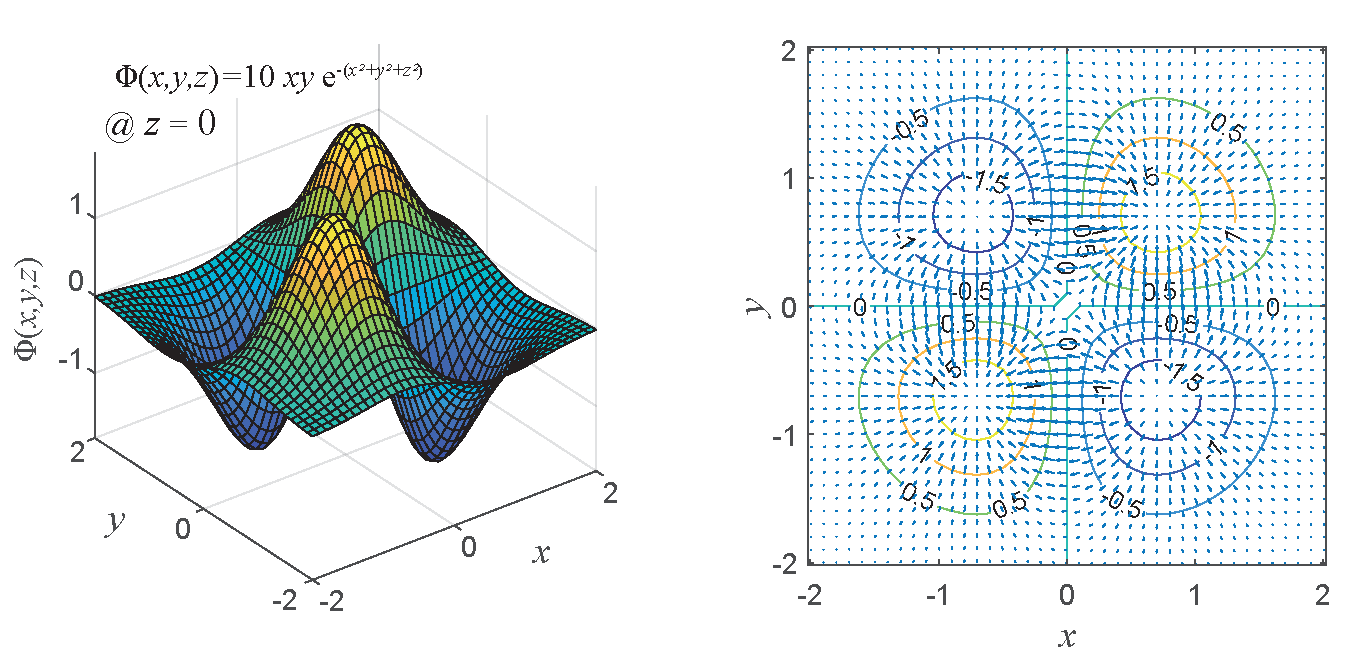
\includegraphics[width=\textwidth]{GradientExample.pdf}
    \caption[Funktion $\Phi = 10 x y \e^{-(x^2+y^2+z^2)}$ und Gradient der Funktion.]
    {Funktion $\Phi = 10 x y \e^{-(x^2+y^2+z^2)}$ und Gradient der Funktion.}
    \label{abb:kontmech_gradientexample1}
\end{figure}

\begin{figure}
    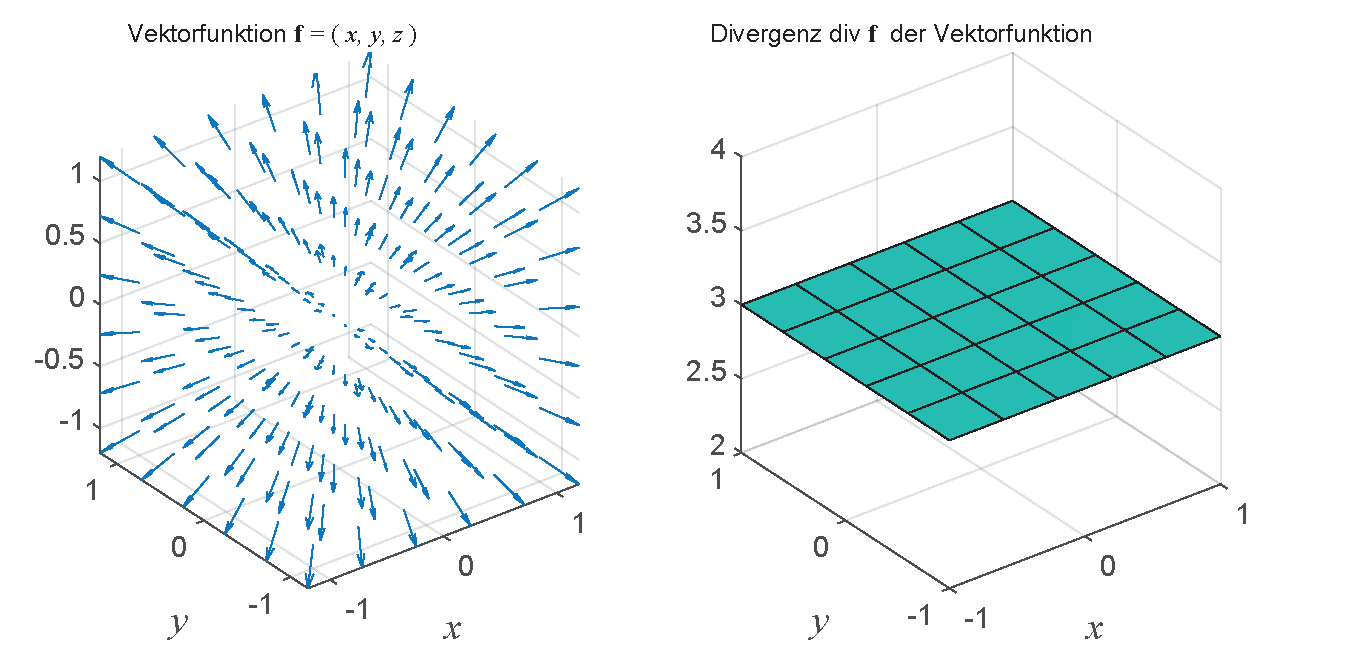
\includegraphics[width=\textwidth]{DivergenceExample.pdf}
    \caption[Vektorfunktion $\vec{f} = ( x, y, z ) $ und Divergenz der Funktion.]
    {Funktion $\vec{f}  = ( x, y, z ) $ und Divergenz der Funktion.}
    \label{abb:kontmech_divexample}
\end{figure}

\newpage
\begin{figure}
    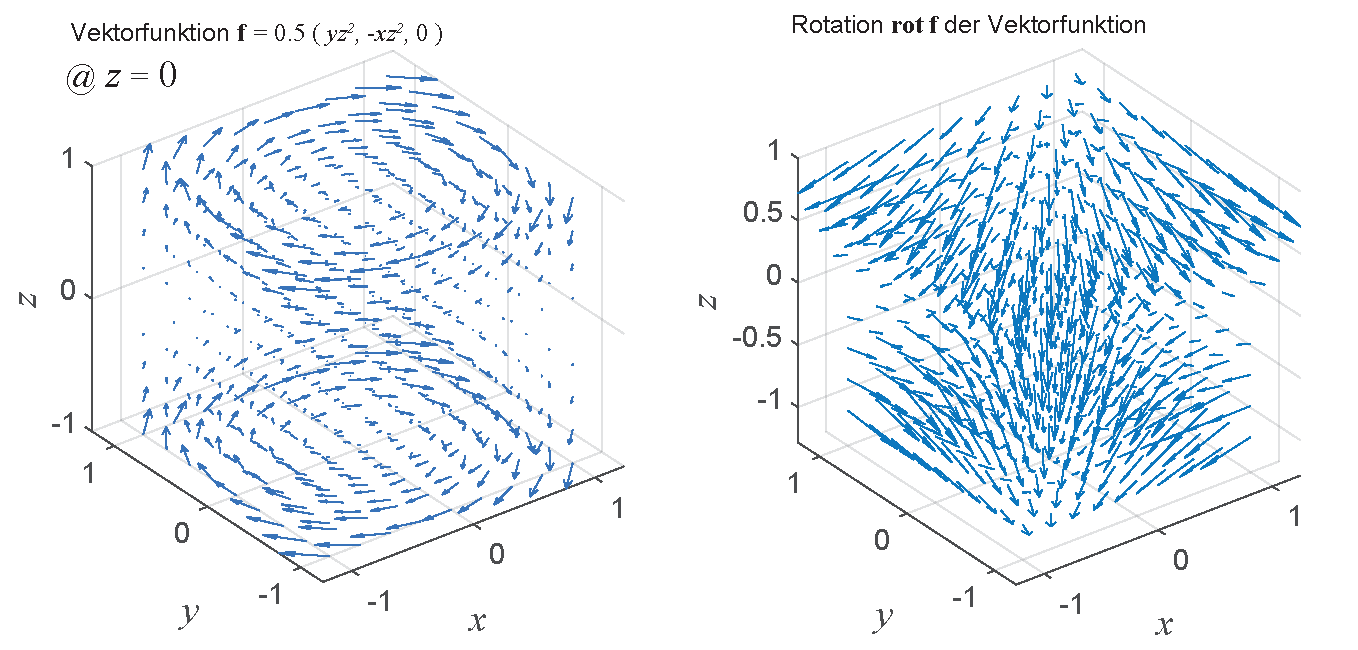
\includegraphics[width=\textwidth]{CurlExample.pdf}
    \caption[Vektorfunktion $\vec{f} = 0.5\,(yz^2, -xz^2, 0)$ und Rotation der Funktion.]
    {Funktion $\vec{f} = 0.5\,(yz^2, -xz^2, 0)$ und Rotation der Funktion.}
    \label{abb:kontmech_curlexample}
\end{figure}



\end{sol} 
\textcolor{blue} {$\rightarrow$ zur} \probref{kontmech_diffoperators}.\\
\noindent\rule[1ex]{\textwidth}{0.5pt}  \newpage  \clearpage

%-----------------------------------------------------------------------------------------------------------

\begin{sol}{prob:kontmech_ueb_vectoranalysis}\label{lsg:kontmech_ueb_vectoranalysis} %�bung2
\textbf{�bungen zur Vektorrechnung und Vektoranalysis}
\begin{enumerate}
    \item [a)] Wir geben exemplarisch die L�sung f�r die Gra�mann\footnote{Hermann G�nther Gra�mann (1809--1877) war ein deutscher Mathematiker und Physiker und einer der wesentlichen Wegbereiter der modernen Vektor- und Tensorrechnung.}-Identit�t \index{Gra�mann-Identit�t}\indexp{Gra�mann,Herrmann} $\vec{a} \times \lk \vec{b} \times \vec{c}\rk $ an, mit $\vec{a} = \lk a_1,a_2,a_3\rk^\intercal,\,\vec{b} = \lk b_1,b_2,b_3\rk^\intercal,\,\vec{c} = \lk c_1,c_2,c_3\rk^\intercal$:
    \begin{enumerate}
        \item [$\alpha$)] Rechnung in \textbf{kartesischen Koordinate}n:
        \begin{align}
            \vec{m} &= \vec{b} \times \vec{c} = 
						\begin{pmatrix}
                m_1 \\
                m_2\\
                m_3
            \end{pmatrix} =
            \begin{vmatrix}
                \vec{e_1} & b_1 & c_1\\
                \vec{e_2} & b_2 & c_2\\
                \vec{e_3} & b_3 & c_3\\
            \end{vmatrix}=
            \begin{pmatrix}
                b_2\,c_3 -b_3\,c_2\\
                b_3\,c_1-b_1\,c_3\\
                b_1\,c_2 -b_2\,c_1
            \end{pmatrix}\nonumber\\ 
            \vec{q} &= \vec{a}\times\vec{m} = 
            \begin{vmatrix}
                 \vec{e_1} & a_1 & m_1\\
                \vec{e_2} & a_2 & m_2\\
                \vec{e_3} & a_3 & m_3\\
            \end{vmatrix} =
            \begin{pmatrix}
                a_2\,m_3-a_3\,m_2\\
                a_3\,m_1-a_1\,m_3\\
                a_1\,m_2-a_2\,m_1
            \end{pmatrix}\nonumber \\
            &= 
            \begin{pmatrix}
                a_2\,b_1\,c_2 - a_2\,b_2\,c_1 - a_3\,b_3\,c_1 + a_3\,b_1\,c_3 \\
                a_3\,b_2\,c_3 - a_3\,b_3\,c_2 - a_1\,b_1\,c_2 + a_1\,b_2\,c_1 \\
                a_1\,b_3\,c_1 - a_1\,b_1\,c_3 - a_2\,b_2\,c_3 + a_2\,b_3\,c_2
            \end{pmatrix}
            = 
            \begin{pmatrix}
                b_1\,\lk a_2\,c_2 +a_3\,c_3\rk - c_1\,\lk a_2\,b_2 + a_3\,b_3\rk \\
                b_2\,\lk a_1\,c_1 +a_3\,c_3\rk - c_2\,\lk a_1\,b_1+a_3\,b_3\rk\\
                b_3\,\lk a_1\,c_1 +a_2\,c_2\rk - c_3\,\lk a_1\,b_1+a_2\,b_2\rk
            \end{pmatrix}\nonumber\\
            &= 
            \begin{pmatrix}
                b_1\,\lk a_i\,c_i\rk - \cancel{b_1\,a_1\,c_1} - c_1\,\lk a_i\,b_i\rk+ \cancel{c_1\,a_1\,b_1}\\
                b_2\,\lk a_i\,c_i\rk - \cancel{b_2\,a_2\,c_2} - c_2\,\lk a_i\,b_i\rk+ \cancel{c_2\,a_2\,b_2}\\
                b_3\,\lk a_i\,c_i\rk - \cancel{b_3\,a_3\,c_3} - c_3\,\lk a_i\,b_i\rk+ \cancel{c_3\,a_3\,b_3}
            \end{pmatrix}
            = \vec{b}\, \lk \vec{a} \,\vec{c} \rk - \vec{c}\, \lk \vec{a}\, \vec{b}\rk  \,.  \label{eq:kontmech_Ueb2_01} 
        \end{align}
        \item [$\beta$)] Rechnung mit \textbf{Levi-Civita-Symbol} und Einsteinscher Summenkonvention
        \begin{align}
            \vec{a}\times\vec{b} = \sum_{i=1}^3\sum_{j=1}^3\sum_{k=1}^3\,\epsilon_{ijk}\,a_i\,b_j\,\vec{e}_k=\epsilon_{ijk}\,a_i\,b_j\,\vec{e}_k \label{eq:kontmech_Ueb2_02}  \,. 
        \end{align}
        Damit:
        \begin{align}
            \vec{a}\times\underbrace{\lk \vec{b}\times\vec{c}\rk}_{\vec{m}} &=\epsilon_{ijk}\,a_i\,m_j\,\vec{e}_k ~~\rightarrow~~
            m_j = \epsilon_{\alpha\beta j}\,b_\alpha\,c_\beta ~~\rightarrow~~
           \lek \vec{a}\times\lk \vec{b}\times \vec{c}\rk \rek_k= \epsilon_{ijk}\,\epsilon_{\alpha\beta j}\,a_i\,b_\alpha\,c_\beta  \,. \label{eq:kontmech_Ueb2_03} 
        \end{align}
        Mit $\epsilon_{ijk} = -\epsilon_{ikj}$ und der Identit�t $ \epsilon_{\alpha\beta j}\,\epsilon_{ikj} = \delta_{\alpha i}\,\delta_{\beta k} - \delta_{\alpha k}\,\delta_{\beta i}$ erhalten wir:
        \begin{align}
            \epsilon_{\alpha\beta j}\,\epsilon_{ijk}\,b_\alpha\,a_i\,c_\beta &= -\epsilon_{\alpha\beta j}\,\epsilon_{ikj}\,b_\alpha\,a_i\,c_\beta 
            = \lk -\delta_{\alpha i}\,\delta_{\beta k} + \delta_{\alpha k}\,\delta_{\beta i}\rk\,b_\alpha\,a_i\,c_\beta \nonumber\\
            &= \delta_{\alpha k}\,b_\alpha\,\delta_{\beta i}\,a_i\,c_\beta - \delta_{\beta k}\,c_\beta\,\delta_{\alpha i}\,a_i\,b_\alpha 
             = \delta_{\alpha k}\,b_k\,a_i\,c_i - \delta_{\beta k}\,c_\beta\,a_i\,b_i \nonumber\\
            &= b_k\,\lk a_i\,c_i\rk -c_k\,\lk a_i\,b_i\rk ~~ \Leftrightarrow ~~\vec{a} \times \lk \vec{b} \times \vec{c}\rk = \vec{b}\,\lk \vec{a}\,\vec{c}\rk -\vec{c}\,\lk\vec{a}\,\vec{b}\rk\,. \label{eq:kontmech_Ueb2_05} 
        \end{align}
    \end{enumerate}
    \item [b)] Wir zeigen die Rechnung exemplarisch f�r \textbf{Zylinderkoordinaten} und bilden die Jacobi-Matrix f�r $q_1 =\rho\,\cos\phi,\,q_2= \rho\,\sin\phi,\,q_3=z$:
    \begin{align}
    \begin{split}
        \mathbb{J} = 
        \begin{pmatrix}
            \frac{\d x}{\d \rho} & \frac{\d x}{\d \phi} & \frac{\d x}{\d z} \\
            \frac{\d y}{\d \rho} & \frac{\d y}{\d \phi} & \frac{\d y}{\d z}\\
            \frac{\d z}{\d \rho} & \frac{\d z}{\d \phi} & \frac{\d z}{\d z}
        \end{pmatrix}
        &=
        \begin{pmatrix}
            \cos\phi & -\rho\,\sin\phi & 0 \\
            \sin\phi & \rho\cos\varphi & 0\\
            0&0&1
        \end{pmatrix}~~~~\text{sowie} ~~~\det \mathbb{J} = \rho
    \end{split} \,. \label{eq:kontmech_Ueb2_07}
    \end{align}
    Wir k�nnen nun schreiben
    \begin{align}
        \begin{pmatrix}
            \D x\\
            \D y\\
            \D z
        \end{pmatrix}
        = 
        \mathbb{J}\,
        \begin{pmatrix}
            \D \rho\\
            \D \phi\\
            \D z
        \end{pmatrix} ~~~\text{und f�r}~\det\mathbb{J}\neq 0: ~~~
        \begin{pmatrix}
            \D \rho\\
            \D \phi
            \D z
        \end{pmatrix}
        =
        \mathbb{J}^{-1}\,
        \begin{pmatrix}
            \D x\\
            \D y\\
            \D z
        \end{pmatrix}  \,. \label{eq:kontmech_Ueb2_09}
    \end{align}
    Die Spalten der Jacobi-Matrix sind gerade die Differentiale $\d\vec{r}/\d q_j$, was uns erlaubt, den neuen Einheitsvektor $\vec{e}_{q_j}$, wie man leicht nachrechnen kann, wie folgt zu schreiben 
    \begin{align}
        \vec{e}_{q_j} = \frac{1}{h_j}\,\frac{\d \vec{r}\lk q_k\rk}{\d q_j} ~~~ \text{mit} ~~~ j=1,2,3 ~~~~~~ \text{mit}~~~h_j =
        \begin{vmatrix}
            \frac{\d \vec{r}}{\d q_j}
        \end{vmatrix}  \,. \label{eq:kontmech_Ueb2_11}
    \end{align}
   Die Gr��en $h_j$ hei�en Skalenfaktoren. Unter Benutzung von \eqref{eq:kontmech_Ueb2_07} finden wir \zb f�r Zylinderkoordinaten mit $\vec{r} = \rho\,\cos\phi\,\vec{e}_x+\rho\,\sin\phi\,\vec{e}_y + z\,\vec{e}_z$ die folgenden Skalenfaktoren:
    \begin{align*}
        h_1 &= |\cos\rho\,\vec{e}_x + \sin\phi\,\vec{e}_y| = 1\,,\\
        h_2 &= |-\rho\,\sin\phi\,\vec{e}_x +\rho\,\cos\phi\,\vec{e}_y| = \rho\,,\\
        h_3 &= |\vec{e}_z| =1\,,
    \end{align*}
    woraus sich leicht die neuen orthogonalen Einheitsvektoren nach \eqref{eq:kontmech_Ueb2_11} berechnen lassen:
    \begin{align}
    \begin{split}
        \vec{e}_\rho &= \lk\cos\varphi,\sin\varphi,0\rk^\intercal\,,\\
        \vec{e}_\phi &= \frac{1}{\rho}\lk -\sin\varphi,\cos\varphi,0\rk^\intercal\,,\\
        \vec{e}_z &= \lk 0,0,1\rk^\intercal\,.
    \end{split}\label{eq:kontmech_Ueb2_12}
    \end{align}
    Wir erkennen hier die Spalten der Jacobi-Matrix wieder. Das Volumenelement, welches \zb f�r die Integration in den neuen Koordinaten ben�tigt wird, berechnet man am einfachsten �ber das Spatprodukt\index{Spatprodukt}. Man erh�lt:
    \begin{align}
    \begin{split}
        \D V &= h_1\,\D q_1\,\vec{e}_{q_1}\,\lk h_2\,\D q_2\,\vec{e}_{q_2} \times h_3\,\D q_3\,\vec{e}_{q_3}\rk = \sum_{j=1}^3\,h_j\,\D q_j = h_a\,h_2\,h_3\,\D q_1\,\D q_2\,\D q_3
    \end{split}  \,. \label{eq:kontmech_Ueb2_13}
    \end{align}
    und speziell f�r Zylinderkoordinaten:
    \begin{align}
        \D V = \rho\,\D\rho\,\D \phi\,\D z \label{eq:kontmech_Ueb2_14}\,.
    \end{align}
    Mit der Beziehung \eqref{eq:kontmech_Ueb2_11} kann man leicht die Beziehung f�r einen Gradienten \bzw den Nabla-Operator $\vec{\nabla}$ aus \eqref{eq:kontmech_nabladef} berechnen:
    \begin{align*}
        \D \Phi &= \frac{\D\Phi}{\d q_j}\,\D q_j = \nabla\Phi\,\D \vec{r}\,,~~~~ \D \vec{r} = \frac{\d \vec{r}}{\d q_j}\,\D q_j\,\vec{e}_j= h_j\,\D q_j\,\vec{e}_{q_j} \\
        \rightarrow ~~ \D \Phi &= \frac{\d \Phi}{\D q_j}\,\D q_j = \nabla\Phi\,h_j\,\D q_j\,\vec{e}_{q_j}  \,. 
    \end{align*}
    Aus dem Vergleich beider Seiten finden wir:
    \begin{align}
        \nabla = \frac{1}{h_j}\,\frac{\d}{\d q_j}\,\vec{e}_{q_j} =  \lk \frac{1}{h_1}\,\frac{\d}{\d q_1},\,\frac{1}{h_2}\,\frac{\d}{\d q_2},\,\frac{1}{h_3}\,\frac{\d}{\d q_3}\rk  \,. \label{eq:kontmech_Ueb2_15}
    \end{align}
    Speziell f�r Zylinderkoordinaten:
    \begin{align}
        \nabla = \lk \frac{\d}{\d \rho},\frac{1}{\rho}\,\frac{\d}{\d\phi},\frac{\d}{\d z }\rk \,. \label{eq:kontmech_Ueb2_17}
    \end{align}
    Aus der leicht zu berechnenden Jacobi-Matrix f�r sph�rische Koordinaten
    \begin{align}
        J = 
        \begin{pmatrix}
            \frac{\d x}{\d r} & \frac{\d x}{\d \theta} &  \frac{\d x}{\d \phi}\\
            \frac{\d y}{\d r} & \frac{\d y}{\d \theta} &  \frac{\d y}{\d \phi}\\
            \frac{\d z}{\d r} & \frac{\d z}{\d \theta} &  \frac{\d z}{\d \phi}
        \end{pmatrix}
        =
        \begin{pmatrix}
            \sin\theta\,\cos\phi & r\,\cos\theta\,\cos\phi & -r\,\sin\theta\,\sin\phi\\
            \sin\theta\,\sin\phi & r\,\cos\theta\,\sin\phi & -r\,\sin\theta\,\cos\phi\\
            \cos\theta & -r\,\sin\theta & 0
        \end{pmatrix}  \,. \label{eq:kontmech_Ueb2_18}
    \end{align}
    \begin{align}
        J^{-1} = 
        \begin{pmatrix}
            \frac{\d r}{\d x} & \frac{\d r}{\d  y} &  \frac{\d r}{\d z}\\
            \frac{\d \theta}{\d x} & \frac{\d \theta}{\d y} &  \frac{\d \theta}{\d z}\\
            \frac{\d \phi}{\d x} & \frac{\d \phi}{\d y} &  \frac{\d \phi}{\d z}
        \end{pmatrix}
        =
        \begin{pmatrix}
            \sin\theta\,\cos\phi & \sin\theta\,\sin\phi & \cos\theta\\
            \frac{1}{r}\,\cos\theta\,\cos\phi & \frac{1}{r}\,\cos\theta\,\sin\phi & -\frac{1}{r}\,\sin\theta \\
            -\frac{1}{r}\,\frac{\sin\phi}{\sin\theta} & \frac{1}{r}\,\frac{\cos\phi}{\sin\theta} & 0
        \end{pmatrix}  \label{eq:kontmech_Ueb2_19}
    \end{align}
    mit 
    \begin{align}
        \det\lk J\rk= r^2\,\sin\theta \label{eq:kontmech_Ueb2_20}
    \end{align}
    finden wir mit 
    \begin{align*}
        h_1 &= 1\,,~~~h_2 = \frac{1}{r\,\sin\theta}\,,~~~h_3 = \frac{1}{r}
    \end{align*}
    schlie�lich
    \begin{align}
        \nabla = \lk \frac{\d}{\d r},\frac{1}{r\,\sin\theta}\,\frac{\d}{\d \phi},\frac{1}{r}\,\frac{\d}{\d\theta}\rk\,. \label{eq:kontmech_Ueb2_21}
    \end{align}
		
		
    Die weiteren \textbf{Differentialoperatoren} $\divv$, $\rotv$, $\Delta$ findet man leicht mit Hilfe des Nabla-Kalk�ls, \zb erhalten wir f�r die Divergenz:
    \begin{align*}
        \divv \vec{f} = \nabla\,\vec{f} = \nabla\,\lk f_j\,\vec{e}_{q_j}\rk = \nabla \,\lk f_j\,\epsilon_{\alpha\beta j}\,\vec{e}_{q_\alpha} \times \vec{e}_{q_\beta}\rk\,.
    \end{align*}
    Dabei haben wir ber�cksichtigt, dass die $\vec{e}_{q_i}$ ein Rechtssystem bilden. Wir wollen diese Beziehung zun�chst f�r $j=1$ auswerten und erhalten mit \eqref{eq:kontmech_Ueb2_15}
    \begin{align*}
        \nabla\,\lk f_1\,\vec{e}_{q_2} \times \vec{e}_{q_3} \rk = \nabla\,\lk f_1\,h_2\,\nabla\,q_2\times h_3\,\nabla\,q_3\rk  \,. 
    \end{align*}
    Wir benutzen:
    \begin{align}
        \nabla q_1 &= \lk\frac{1}{h_1}\,\frac{\d q_1}{\d q_1},\underbrace{\frac{1}{h_2}\,\frac{\d q_1}{\d q_2}}_{=0},\underbrace{\frac{1}{h_3}\,\frac{\d q_1}{\d q_3}}_{=0}\rk~~\rightarrow ~~~~ h_1\,\nabla\,q_1 = \vec{e}_{q_1}  \,. 
    \end{align}
    \begin{align*}
        \nabla\,\lk f_1\,h_2\,\nabla\,q_2\times h_3\,\nabla\,q_3\rk &= \nabla\,\lk f_1\,h_2\,h_3 \,\lk \nabla\,q_2\times\nabla\,q_3\rk \rk \\
        &= \nabla\,\lk f_1\,h_2\,h_3\rk\,\cdot \lk \nabla q_2\times\nabla\,q_3\rk + f_1\,f_2\,h_3\,\underbrace{\nabla\,\lk \nabla\,q_2\times\nabla\,q_2\rk}_{=0}\\
        &= \nabla\,\lk f_1\,h_2\,h_3\rk\cdot\lk\frac{\vec{e}_2}{h_2}\times\frac{\vec{e}_3}{h_3}\rk = \nabla\,\lk f_1\,h_2\,h_3\rk\cdot\frac{\vec{e}_1}{h_2\,h_3}r\\
        &= \lek \frac{1}{h_1}\,\frac{\d \lk f_1 h_2 h_3 \rk}{\d q_1}\,\vec{e}_1+\ldots\,\vec{e}_2+\ldots\,\vec{e}_3\rek\cdot\frac{\vec{e}_1}{h_2\,h_3} = \frac{1}{h_1\,h_2\,h_3}\,\frac{\d}{\d q_1}\,\lk f_1\,h_2\,h_3\rk  \,. 
    \end{align*}
    Analog f�r $j=2,3$ in \eqref{eq:kontmech_Ueb2_15} erh�lt man:
    \begin{align}
        \divv \vec{f} &= \nabla\,\vec{f} = \frac{1}{h_1\,h_2\,h_3}\,\lek \frac{\d}{\d q_1}\,\lk h_2\,h_3\,f_1\rk + \frac{\d}{\d q_2}\,\lk h_3\,h_1\,f_2\rk + \frac{\d}{\d q_3}\,\lk h_1\,h_2\,f_3\rk\rek \,.\label{eq:kontmech_Ueb2_23}  
    \end{align}
    
		Alternativ kann die \textbf{Divergenz} auch mit Hilfe des \textbf{Integralsatzes von Gau�} berechnet werden:
    \begin{align*}
        \iiint_{\text{Vo}}\divv\,\vec{f}\,\D V = \iint_{\d \text{Vo}}\,\lk \vec{f}\,\vec{n}\rk\,\D A \,.
    \end{align*}
    Das Volumen, �ber das integriert wird, soll ein sehr kleines Parallelepiped sein, das von den kleinen krummlinigen Rechtecken in den drei Koordinatenebenen $q_1,q_1+\D q_1;q_2,q_2 +\D q_2;q_3,q_3 + \D q_3$ begrenzt wird; die Seitenl�ngen dieser Rechtecke sind durch $\D s_1,\D s_2,\D s_3$ gegeben. \\
    Das Volumen ist so klein, dass sich das Vektordifferential darin kaum �ndert und daher vor das Integral gezogen werden kann; das verbleibende Integral ist dann das kleine Volumenelement $\D V$. Damit ergibt sich folgender Ausdruck f�r die Divergenz:
    \begin{align}
        \divv\,\vec{f} = \frac{1}{\D V}\,\iint_{\d \text{Vo}}\,\lk \vec{f}\,\vec{n}\rk\,\D A := I_1+I_2+I_3\,.\label{eq:kontmech_Ueb2_24}
    \end{align}
    Das Oberfl�chenintegral $I$ wird n�herungsweise berechnet, indem der Wert von $\lk \vec{f}\,\vec{n}\rk$ mit der Gr��e der Fl�che multipliziert wird. Dann ergibt sich f�r die zwei Fl�chen $q_3$ und $q_3 + \D q_3$:
    \begin{align*}
        \text{Fl�che}\,q_3:\,&-\lk f_3\,h_1\,h_2\rk_{q_3}\,\D q_1\,\D q_2\,,\\
         \text{Fl�che}\,q_3 + \D q_3:\,&+\lk f_3\,h_1\,h_2\rk_{q_3+\D q_3}\,\D q_1\,\D q_2 \\
         &~~=\lk f_3\,h_1\,h_2\rk_{q_3}\,\D q_1\,\D q_2 + \frac{\d}{\d q_3}\,\lk f_3\,h_1\,h_2\rk_{q_3}\,\D q_3\,\D q_2\,\D q_2\,.
    \end{align*}
    Die Indices $q_3$ \bzw $q_3+\D q_3$ geben an, dass die Funktion in der Klammer an $q_3$ \bzw $q_3 + \D q_3$ zu berechnen ist. Die Summer obiger Terme gibt dann:
    \begin{align*}
        I_3= \frac{\d}{\d q_3}\,\lk f_3\,h_1\,h_2\rk\,\D q_1\,\D q_2\,\D q_3\,.
    \end{align*}
    Analog berechnet man die Integrale $I_1$ und $I_2$:
    \begin{align*}
        I_1&= \frac{\d}{\d q_1}\,\lk f_1\,h_2\,h_3\rk\,\D q_1\,\D q_2\,\D q_3\,,~~~I_2= \frac{\d}{\d q_2}\,\lk f_2\,h_2\,h_3\rk\,\D q_1\,\D q_2\,\D q_3\,.
    \end{align*}
    Die Summe $I_1+I_2+I_3$ wird durch das infinitesimale Volumen $\D V = h_1\,h_2\,h_3\,\D q_1\,\D q_2\,\D q_3$ dividiert. Dabei k�rzen sich die Differentiale und man erh�lt wieder den Ausdruck f�r die Divergenz, der nat�rlich mit \eqref{eq:kontmech_Ueb2_23} �bereinstimmt:
    \begin{align}
        \divv\,\vec{f} = \frac{1}{h_1\,h_2\,h_3}\,\lek \frac{\d}{\d q_1}\,\lk f_1\,h_2\,h_3\rk+\frac{\d}{\d q_2}\,\lk f_2\,h_1\,h_3\rk + \frac{\d}{\d q_3}\,\lk f_3\,h_2\,h_3\rk\rek \,. \label{eq:kontmech_Ueb2_25}
    \end{align}
		
    Eine Herleitung der \textbf{Rotation} findet man entsprechend �ber den \textbf{Integralsatz von Stokes}.
    \begin{align}
        \rotv\,\vec{f} = \iint_{\text{Ar}}\rotv\,\vec{f}\,\D \vec{A} = \oint\limits_{\d \text{Ar}}\vec{f}\,\D \vec{r}\,.\label{eq:kontmech_Ueb2_26}
    \end{align}
    Wir finden:
    \begin{align}
        \rotv\,\vec{f} = \nabla\times\vec{f} = \frac{1}{h_1\,h_2\,h_3}\,
        \begin{vmatrix}
            h_1\,\vec{e}_{q_1} & h_2\,\vec{e}_{q_2} & h_3\,\vec{e}_{q_3} \\
            \frac{\d}{\d q_1} & \frac{\d}{\d q_2} & \frac{\d}{\d q_3} \\
            h_1\,f_1 & h_2\,f_2 & h_3\,f_3
        \end{vmatrix} \,. \label{eq:kontmech_Ueb2_27}
    \end{align}
    
		F�r den \textbf{Laplace-Operator} $\Delta$ finden wir:
    \begin{align}
        \Delta\Phi = \nabla^2\Phi =\,&\frac{1}{h_1\,h_2\,h_3}\,\lek \frac{\d}{\d q_1}\,\lk \frac{h_2\,h_3}{h_1}\,\frac{\d \Phi}{\d q_1}\rk + \frac{\d}{\d q_2}\,\lk \frac{h_1\,h_3}{h_2}\,\frac{\d \Phi}{\d q_2}\rk + \frac{\d}{\d q_3}\,\lk \frac{h_2\,h_3}{h_3}\,\frac{\d \Phi}{\d q_3}\rk\rek \,.
    \end{align}\\
    
	 Zusammenfassend finden wir f�r \textbf{sph�rische Koordinaten}
    \begin{subequations}
    \begin{align}
        \nabla\Phi &= \frac{\d\Phi}{\d r}\,\hat{\vec{e}}_r + \frac{1}{r}\,\frac{\d\Phi}{\d\theta}\,\hat{\vec{e}}_\theta + \frac{1}{r\,\sin\theta}\,\frac{\d\Phi}{\d\phi}\,\hat{\vec{e}}_\phi  \,,\\
        \nabla\,\vec{f} &= \frac{1}{r^2}\,\frac{\d}{\d r}\,\lk r^2\,f_r\rk + \frac{1}{r\,\sin\theta\,\frac{\d}{\d \theta}}\,\lk \sin\theta\,f_\theta\rk + \frac{1}{r\,\sin\theta}\,\frac{\d f_\phi}{\d \phi}  \,,\\
        \nabla\times\vec{f} &= \frac{1}{r^2\,\sin\theta}\,
        \begin{vmatrix}
            \hat{\vec{e}}_r &  r\,\hat{\vec{e}}_\theta & r\,\sin\theta\,\hat{\vec{e}}_\phi\\
            \frac{\d}{\d r} & \frac{\d}{\d \theta} & \frac{\d}{\d \phi}  \,,\\
            f_r & r\,f_\theta & r\,\sin\theta\,f_\phi
        \end{vmatrix} \\
        \Delta\Phi &= \frac{1}{r^2}\,\frac{\d}{\d r}\,\lk r^2\,\frac{\d \Phi}{\d r}\rk + \frac{1}{r^2\,\sin\theta}\,\frac{\d}{\d\theta}\,\lk\sin\theta\,\frac{\d \Phi}{\d \theta}\rk + \frac{1}{r^2\,\sin^2\theta}\,\frac{\d^2\Phi}{\d \phi^2}  \,. 
    \end{align}\label{eq:kontmech_Ueb2_28}
    \end{subequations} 
    und analog f�r die \textbf{Zylinderkoordinaten}:
    \begin{subequations}
    \begin{align}
        \nabla\Phi &= \frac{\d\Phi}{\d \rho}\,\hat{\vec{e}}_\rho + \frac{1}{\rho}\,\frac{\d\Phi}{\d\phi}\,\hat{\vec{e}}_\phi + \frac{\d\Phi}{\d z}\,\hat{\vec{e}}_x \,,\\
        \nabla\,\vec{f} &= \frac{1}{\rho}\,\frac{\d}{\d \rho}\,\lk\rho\,f_\rho\rk + \frac{1}{\rho}\,\frac{\d f_\phi}{\d \phi} + \frac{\d f_z}{\d z} \,,\\
        \nabla\times\vec{f}&= \frac{1}{\rho}\,
        \begin{vmatrix}
            \hat{\vec{e}}_\rho & \rho\,\hat{\vec{e}}_\phi & \hat{\vec{e}}_z \\
            \frac{\d}{\d \rho} & \frac{\d}{\d \phi} & \frac{\d}{\d z} \\
            f_\rho & \rho\,f_\phi & f_z
        \end{vmatrix}  \,,\\
        \nabla^2\,\Phi &= \frac{1}{\rho}\,\frac{\d}{\d\rho}\,\lk\rho\,\frac{\d\Phi}{\d \rho} + \frac{1}{\rho^2}\,\frac{\d^2\Phi}{\d \phi^2} + \frac{\d^2\Phi}{\d z^2}\rk  \,.
    \end{align}\label{eq:kontmech_Ueb2_29}
    \end{subequations}
    \item[c)] Wir berechnen nun noch die \textbf{Geschwindigkeit und Beschleunigung in Zylinderkoordinaten}:
    \begin{align}
    \begin{split}
        \vec{r} &= \rho\,\vec{e}_\rho + z\,\vec{e}_z  \,,\\
        \dot{\vec{r}} &= \dot{\rho}\,\vec{e}_\rho+\dot{z} \vec{e}_z + \rho\,\dot{\vec{e}}_\rho + z\,\dot{\vec{e}}_z = \dot{\rho}\,\vec{e}_\rho + \dot{z}\,\vec{e}_z + \rho\,
        \underbrace{
        \begin{pmatrix}
            -\sin\varphi\\
            \cos\varphi\\
            0
        \end{pmatrix}
        }_{=\vec{e}_\phi}\,\dot{\phi} +0 = \dot{\rho}\,\vec{e}_\rho  + \rho\,\dot{\phi} \,\vec{e}_\phi + \dot{z}\,\vec{e}_z  \,.
    \end{split}\label{eq:kontmech_Ueb2_30}
    \end{align}
    \begin{align}
    \begin{split}
        \ddot{\vec{r}} &= \ddot{\rho}\,\vec{e}_\rho + \dot{\rho}\,\dot{\phi}\,\vec{e}_\rho + \rho\,\ddot{\phi}\,\vec{e}_\phi + \ddot{z}\,\vec{e}_z +\dot{\rho}\,\dot{\vec{e}}_\rho + \rho\,\dot{\phi}\,\dot{\vec{e}}_\phi~~~\text{mit}~~~
        \dot{\vec{e}}_\rho = 
        \underbrace{
        \begin{pmatrix}
            -\sin\varphi\\
            \cos\varphi\\
            0
        \end{pmatrix}
        }_{=\vec{e}_\phi}\,\dot{\phi} ~~~\text{und}~~~\dot{\vec{e}}_\phi = 
        \underbrace{
        \begin{pmatrix}
            -\rho\,\sin\phi\\
            \rho\,\cos\phi\\
            0
        \end{pmatrix}
        }_{=-\vec{e}_\rho\,\dot{\phi}}\,\dot{\phi}\\
        &= \lk \ddot{\rho} -\rho\,\dot{\phi}^2\rk \, \vec{e}_\rho + \lk 2\dot{\rho}\,\dot{\phi} + \rho\,\ddot{\phi}\rk\,\vec{e}_\phi + \ddot{z}\,\vec{e}_z  \,.
    \end{split}\label{eq:kontmech_Ueb2_31}
    \end{align}
\end{enumerate}
\end{sol} 
\textcolor{blue} {$\rightarrow$ zur} \probref{kontmech_ueb_vectoranalysis}.\\
\noindent\rule[1ex]{\textwidth}{0.5pt}  \newpage  \clearpage


%-----------------------------------------------------------------------------------------------------------

\begin{sol}{prob:kontmech_integralsaetze}\label{lsg:kontmech_integralsaetze} %�bung3
\textbf{Integrals�tze der Vektoranalysis}
\begin{enumerate}
    \item [1)]
    \begin{align*}
        \vec{f}_1\lk \vec{r}\rk &= 0.5\,
        \begin{pmatrix}
            y\,z^2\\
            -x\,z^2\\
            0
        \end{pmatrix} 
				~~\rightarrow~~ \divv \vec{f}_1\lk\vec{r}\rk = 0 \quad \rotv \vec{f}_1\lk\vec{r}\rk = 
        \begin{pmatrix}
            x\,z\\
            y\,z\\
            -z^2
        \end{pmatrix} \\
        \vec{f}_2\lk \vec{r}\rk &= 
        \begin{pmatrix}
            0\\
            2x\,z + 3y^2\\
            4y\,z^2
        \end{pmatrix}
       ~~\rightarrow~~\divv \,\vec{f}_2\lk\vec{r}\rk = 0+6y+8y\,z = y\,\lk 3+4z\rk \quad  \rotv \vec{f}_2\lk\vec{r}\rk = 
        \begin{pmatrix}
            -2x+4z^2\\
            0\\
            2z
        \end{pmatrix}
    \end{align*}
    \begin{enumerate}
        \item [a)] \underline{Integralsatz von Gau� f�r $\vec{f}_1$}
        \begin{align*}
            \int\limits_{\text{Vo}} \divv \vec{f}_1\,\D V = 0 = \iint\limits_{\d \text{Vo}}\vec{f}_1\,\D \vec{A} = I
        \end{align*}
        Wir betrachten den Einheitskubus $V_o = \lek 0,1;0,1;0,1\rek$ mit den Au�enfl�chen:
        \begin{align*}
            A1:\,z=0,\,x=\lek 0,1\rek,\,y=\lek 0,1\rek ~~~~ \lk -\vec{e}_z-\text{Richtung}\rk \\
            A2:\,z=1,\,x=\lek 0,1\rek,\,y=\lek 0,1\rek ~~~~ \lk +\vec{e}_z-\text{Richtung}\rk\\
            A3:\,x=0,\,y=\lek 0,1\rek,\,z=\lek 0,1\rek ~~~~ \lk -\vec{e}_x-\text{Richtung}\rk\\
            A4:\,x=1,\,y=\lek 0,1\rek,\,z=\lek 0,1\rek ~~~~ \lk +\vec{e}_x-\text{Richtung}\rk \\
            A5:\,y=0,\,x=\lek 0,1\rek,\,z=\lek 0,1\rek ~~~~ \lk -\vec{e}_y-\text{Richtung}\rk\\
            A6:\,y=1,\,x=\lek 0,1\rek,\,z=\lek 0,1\rek ~~~~ \lk +\vec{e}_y-\text{Richtung}\rk
        \end{align*}
        \begin{align*}
            I_1 &= \int\limits_0^1\int\limits_0^1\,\vec{f}_1\,\lk z=0,x,y\rk\,\vec{e}_z\,\vec{e}_z\,\D x \D y = 0\quad\quad
            I_2 = \int\limits_0^1\int\limits_0^1\,\lk y\,z^2\,\vec{e}_x - x\,z^2\,\vec{e}_y\rk\,\vec{e}_z\,\D x \D y = 0\\
            I_3 &= \int\limits_0^1\int\limits_0^1\,y\,z^2\,\vec{e}_x\,\lk -\vec{e}_x\rk\,\D z\,D y = -\frac{1}{6}\quad\quad\quad
            I_4 = \int\limits_0^1\int\limits_0^1\,y\,z^2\,\vec{e}_x\,\lk \vec{e}_x\rk\,\D y\,D z = \frac{1}{6}\\
            I_5 &= \int\limits_0^1\int\limits_0^1\,-x\,z^2\,\vec{e}_y\,\lk - \vec{e}_y\rk\,\D x\,D z = \frac{1}{6}\quad\quad\quad
            I_6 = \int\limits_0^1\int\limits_0^1\,-x\,z^2\,\vec{e}_y\,\lk \vec{e}_y\rk \D x \D z = -\frac{1}{6}\\
            I &= \sum_{i=1}^6\,I_i = 0\\
        \end{align*}
        \item [b)] \underline{Integralsatz von Gau� f�r $\vec{f}_2$}
        \begin{align*}
            \int\limits_{\text{Vo}} \divv \vec{f}_2 \,\D V &= \int\limits_0^1\int\limits_0^1\int\limits_0^1 \lk 6y + 8y\,z\rk\,\D x \D y \D z = \int\limits_0^1\int\limits_0^1\lk 6y+8y\,z\rk\,\D y \D z = \int\limits_0^1\lk 3y^2+4y^2\,z\rk\, \D z = 5
        \end{align*}
        Wir betrachten wiederum den Einheitskubus mit den 6 Au�enfl�chen:
        \begin{align*}
             I_1 &= \int\limits_0^1\int\limits_0^1 -4y\,z^2 \D x \D y \,\Big|_{z=0} = 0\quad\quad\quad\quad
             I_2 = \int\limits_0^1\int\limits_0^1 4y\,z^2 \,\Big|\D x \D y =2\\
             I_3 &= \int\limits_0^1\int\limits_0^1 0\,\vec{e}_x\,\lk -\vec{e}_x\rk \,\D y\D z = 0\quad\quad\quad\quad
             I_4 = \int\limits_0^1\int\limits_0^1 0\,\vec{e}_x\,\lk +\vec{e}_x\rk \D y \D z = 0 \\
             I_5 &= \int\limits_0^1\int\limits_0^1 2x\,z\,\vec{e}_y\,\lk -\vec{e}_y\rk \D x \D z = -\frac{1}{2}\quad\quad
             I_6 = \int\limits_0^1\int\limits_0^1\lk 2x\,z+3\rk\,\vec{e}_y\,\lk +\vec{e}_y\rk \D x \D z = \frac{7}{2}\\
             I &= \sum_{i=1}^6 I_i = 2-\frac{1}{2}+3+\frac{1}{2} = 5
        \end{align*}
        Man sieht, dass manchmal die Volumenintegrale �ber die Divergenz oft einfacher zu berechnen sind als die Oberfl�chenintegrale, manchmal aber auch umgekehrt.
    \end{enumerate}
    \item[2)] F�r den Satz von Stokes betrachten wir exemplarisch das Einheitsquadrat bei $z=1$ parallel zur $x-y$-Ebene.
    \begin{enumerate}
        \item [a)] Funktion $\vec{f}_1$:
        \begin{align*}
        \int\limits_\text{Ar} \rotv \vec{f}_1\,\D \vec{A} = \int\limits_0^1\int\limits_0^1 -z^2\,\vec{e}_z\,\vec{e}_z \D x \D y \,\Big|_{z=1} =-1
        \end{align*}
        F�r das Linienintegral haben wir vier Abschnitte.
        \begin{align*}
            \int\limits_{\d \text{Ar}} \vec{f}_1 \D \vec{r} = I_1 + I_2+I_3+I_4
        \end{align*}
        \begin{align*}
            I_1: y=0,\,x=\lek 0,1\rek\quad\quad I_2: x=1,\,y=\lek 0,1\rek\quad \quad 
            I_3: y=1,\,x=\lek 0,1\rek\quad\quad I_4: x=0,\,y=\lek 0,1\rek\\
        \end{align*}
        \begin{align*}
            I_1 &= \int\limits_0^1 \frac{1}{2}\,y\,z^2\,\vec{e}_x\,\vec{e}_x\, \D x\,\Big|_{z=1,y=0} = 0\quad\quad\quad\quad\quad\quad
            I_2 = \frac{1}{2}\,\int\limits_0^1 -x\,z^2,\vec{e}_y\,\vec{e}_y\,\D y\,\Big|_{x,z=1} = \frac{1}{2}\,y\,\Big|_0^1 =-\frac{1}{2}\\
            I_3 &= \frac{1}{2}\,\int\limits_1^0 y\,z^2,\vec{e}_x\,\vec{e}_x\,\D x\,\Big|_{y,z=1} = \frac{1}{2}\,x\,\Big|_1^0 =-\frac{1}{2}\quad\quad
            I_4 = \frac{1}{2}\,\int\limits_0^1 -x\,z^2,\vec{e}_y\,\vec{e}_y\,\D y\,\Big|_{x=0,z=1} = 0\,y\,\Big|_1^0 =0\\
            I &= \sum_{i=1}^4 I_i = -1
        \end{align*}
        \item [b)] Funktion $\vec{f}_2$:
        \begin{align*}
            \int\limits_\text{Ar} \rotv \vec{f}_2 \,\D \vec{A} = \int\limits_0^1 \int\limits_0^1 2z \, \vec{e}_z \vec{e}_z \,\D x \D y =2
        \end{align*}
        \begin{align*}
            I_1 &= \int\limits_0^1 0\,\vec{e}_x\,\vec{e}_x\,\D x = 0\quad\quad\quad
            I_2 = \int\limits_0^1\lk 2x\,z+3y^2\rk\,\vec{e}_y\,\vec{e}_y \D y\,\Big|_{x,z=1} = 2y+y^3\,\Big|_0^1 = 3 \\
            I_3 &= \int\limits_1^0 0\,\vec{e}_x\,\vec{e}_x\,\D x = 0\quad\quad\quad
            I_4 = \int\limits_1^0 3y^2\,\vec{e}_y\,\vec{e}_y\,\D y\,\Big|_{x,z=1} = -\frac{3}{3}\,y^3\,\Big|_1^0= -1 \\
            I&= \sum_{i=0}^4\,I_i =2
        \end{align*}
    \end{enumerate}
    \item [3)] Die Divergenz von $\vec{f}\lk \vec{r}\rk$ ist gegeben durch:
    \begin{align*}
        \divv \begin{pmatrix}
            2x+3z\\
            -x\,z-\\
            y^2+2z
        \end{pmatrix} =
        \lk 2+\lk -1\rk +2\rk =3\,.
    \end{align*}
    Das Volumen der Kugel mit Radius 3 ist $\frac{4}{3}\,\pi\,3^3$, so dass der Gau�sche Integralsatz
    \begin{align*}
        \int\limits_{\d v_0}\vec{f}\,\D \vec{A} = \int\limits_{v_0} 3\,\D v = \cancel{3}\,\frac{4}{\cancel{3}}\,\pi\,3^3  = 108\,\pi
    \end{align*}
     ergibt. Hier ist offensichtlich, wie viel einfacher die Berechnung �ber das Volumenintegral ist. 
    \item [4)] F�r ein Vektorfeld $\vec{f}$ welches die Divergenz $\divv \vec{f} = 1$ hat, kann man das Volumen �ber
    \begin{align*}
        V=\int\limits_\text{Vo} \,\D V = \int\limits_\text{Vo} \divv \vec{f}\,\D V = \int\limits_{\d \text{Vo}}\,\vec{f}\,\D \,\vec{A}
    \end{align*}
    durch das Oberfl�chenintegral berechnen.
    \begin{enumerate}
        \item [i)] Wir nehmen als Funktion $\vec{f} = \frac{1}{2}\,\lk x,y,0\rk$ und k�nnen in dem wir Zylinderkoordinaten verwenden f�r das Volumen schreiben:
        \begin{align*}
            V = \int\limits_{\d \text{Vo}}\vec{f}\,\D \vec{A} = \int\limits_0^h\,\underbrace{\frac{1}{2}\,\rho\lk z\rk}_{f\lk z\rk}\,\underbrace{2\pi\,\rho\lk z\rk\,\D z}_{\D A}
        \end{align*}
        Die Deckfl�chen geben keine Beitrag, da $f_z = 0$ ist.\\
        Die Integration ergibt mit $\rho\lk z\rk = R\,\lek 1+a\,\sin\lk\frac{\pi\,z}{h}\rk\rek^{\frac{1}{2}}$
        \begin{align*}
            V&= \pi\,R^2\,\int\limits_0^h\lek 1+a\,\sin\lk\frac{\pi\,z}{h}\rk\rek\,\D z = \pi\,R^2\,h\,\lk 1+\frac{2a}{\pi}\rk
        \end{align*}
        \item [ii)]
        \begin{align*}
            \frac{x^2}{a^2} + \frac{z^2}{b^2} = \frac{\rho^2}{a^2} + \frac{z^2}{b^2} =1 ~~~~ \rightarrow ~~~~ \rho^2 = a^2\,\lk 1-\frac{z^2}{b^2}\rk
        \end{align*}
        \begin{align*}
            V &= \frac{1}{2}\,\int\limits_{-h}^h\,a^2\,\lk 1-\frac{z^2}{b^2}\rk\,2\pi\,\D z = \pi\,a^2\,\lek z-\frac{1}{3}\,\frac{z^3}{b^2}\rek_{-h}^h = 2\pi\,a^2\,h\,\lek 1-\frac{1}{3}\,\frac{h^2}{b^2}\rek
        \end{align*}
        F�r $z=h=2$ soll der Radius $=1$ sein
        \begin{align*}
            R^2 = \rho^2 = a^2 \,\lk 1-\frac{4}{b^2}\rk  \stackrel{!}{=}1
        \end{align*}
        Maximale Dicke bei $z=0$ soll $2\cdot 1.5$ sein
        \begin{align*}
            \rho^2 = a^2 \stackrel{!}{=}1.5^2 ~~~~\rightarrow ~~~~ a=1.5 ~~~~ \rightarrow ~~~~ b=2\,\sqrt{\frac{1}{1-\frac{1}{2.25}}}\approx 2.6833
        \end{align*}
        Mit diesen Werten ergibt sich ein Volumen von $\approx \SI{23}{\cubic\metre}$
    \end{enumerate}
		Die Berechnungen zum Volumen des Fasses unter Benutzung des Satzes von Gau� finden sich im \mscr{}\, \mlkontmechref{FassFormelGauss.m}.
\end{enumerate}


\end{sol} 
\textcolor{blue} {$\rightarrow$ zur} \probref{kontmech_integralsaetze}.\\
\noindent\rule[1ex]{\textwidth}{0.5pt}  \newpage  \clearpage

%-----------------------------------------------------------------------------------------------------------

\begin{sol}{prob:kontmech_bernoulli}\label{lsg:kontmech_bernoulli} %�bung4
\textbf{Bernoulli-Gleichung}\\ \\

Wir gehen von der Euler-Gleichung
\begin{equation}
  \varrho \lk \lk \vec{v} \cdot \nabla \rk \vec{v} + \frac{\partial}{\partial t}
  \vec{v} \rk = \vec{f}_\text{V}  + \vec{f}_\text{R} - \vec{\nabla} p \; .
  \label{eq:kontmech_exEulerGleichung}
\end{equation}
aus. Die Bernoulli-Gleichung gilt, wie bereits in Kapitel
\ref{kap:kontmech_EulerGl} erw�hnt wurde, in dem Fall, in dem keine
Reibung auftritt, also $\vec{f}_\text{R} = \vec{0}$. Weiterhin treten
auch keine Volumenkr�fte auf, $\vec{f}_\text{V} = \vec{0}$ und es wird
ausschlie�lich der Fall einer station�ren Str�mung betrachtet, also
\begin{equation*}
\frac{\partial}{\partial t} \vec{v} = \vec{0} \; .
\end{equation*}
Dies f�hrt auf 
\begin{equation}
  \varrho \lk \vec{v} \cdot \nabla \rk \vec{v}  = - \vec{\nabla} p \; .
  \label{eq:kontmech_exEulervereinfacht}
\end{equation}

Nun ber�cksichtigen wir, dass die Euler-Gleichung nur f�r eine Str�mung in
eine feste Richtung gilt. Wir k�nnen das Koordinatensystem ferner so w�hlen, dass die Geschwindigkeit nur eine Komponente in $x$-Richtung hat:
\begin{equation*}
   \vec{v} = v_x \veceX
\end{equation*}
Damit haben wir es nur mit einem Geschwindigkeitsgradienten in
$x$-Richtung zu tun. Daraus l�sst sich aber mit Gleichung
\eqref{eq:kontmech_exEulervereinfacht} schlie�en, dass auch der Druckgradient
nur in $x$-Richtung vorliegt,
\begin{equation*}
  \vec{v}(\vec{r}) = v_x(x) \veceX \; , \qquad
  \vec{p}(\vec{r}) = \vec{p}(x) \; .
\end{equation*}
Es reicht also eine eindimensionale Beschreibung
\begin{equation}
  \varrho \lk v_x(x) \frac{\partial}{\partial x} \rk v_x(x)
  = - \frac{\partial p(x)}{\partial x} \; .
  \label{eq:kontmech_exEuler1D}
\end{equation}

Nun ber�cksichtigen wir noch, dass
\begin{equation*}
  \lk v_x(x) \frac{\partial}{\partial x} \rk v_x(x)
  = v_x(x) \frac{\partial v_x(x)}{\partial x}
  = \frac{1}{2} \frac{\partial v_x(x)^2}{\partial x}
  = \frac{\partial}{\partial x} \lk \frac{1}{2} v_x(x)^2 \rk \; .
\end{equation*}

Damit l�sst sich die eindimensionale Gleichung \eqref{eq:kontmech_exEuler1D}
zusammenfassen zu
\begin{align*}
  \frac{\partial}{\partial x} \lk \frac{\varrho}{2} v_x(x)^2 \rk
  + \frac{\partial}{\partial x} p(x) = 0
  \intertext{oder}
  \frac{\partial}{\partial x} \lk \frac{\varrho}{2} v_x(x)^2 +  p(x) \rk
  = 0 \; .
\end{align*}
Daraus l�sst sich schlie�en, dass der Term in der Klammer entlang der
Raumrichtung $x$ konstant sein muss,
\begin{equation*}
  \frac{\varrho}{2} v_x(x)^2 +  p(x) = \con
\end{equation*}
Dies ist genau die Aussage der Bernoulli-Gleichung.

\end{sol} 
\textcolor{blue} {$\rightarrow$ zur} \probref{kontmech_bernoulli}.\\
\noindent\rule[1ex]{\textwidth}{0.5pt}  \newpage  \clearpage

%-----------------------------------------------------------------------------------------------------------

\begin{sol}{prob:kontmech_magnus}\label{lsg:kontmech_magnus} %�bung5
\textbf{Magnus-Effekt, Flettner-Rotoren}\\ \\

Rotiert ein Zylinder (eine Kugel betrachten wir sp�ter in Band III) um eine senkrecht zu einer laminaren Str�mung (Geschwindigkeit $\vec{v}$) gerichteten Achse mit der Winkelgeschwindigkeit $\vec{\omega}_0$, so werden an der Grenzfl�che des K�rpers die Elemente des Fluids mitgenommen. Es ergibt sich dann aus dem laminare Str�mungsprofil (berechenbar als Str�mungsprofil einer Potentialstr�mung, \figref{kontmech_magnus01}\,a) durch �berlagerung der Grenzschichtstr�mung (\figref{kontmech_magnus01}\,b) ein Geschwindigkeitsprofil nach \figref{kontmech_magnus01}\,c.
Offensichtlich ist an der Seite, wo Stromrichtung und Rotationsrichtung �bereinstimmen, die Geschwindigkeit der Fluidelemente gr��er als auf der anderen Seite. Das f�hrt nach dem Bernoulli-Gesetz dazu, dass es auf der Seite, auf der die Fluidelemente mitbewegt werden, zu einer Druckerniedrigung kommt (im Bild links)  und entsprechend umgekehrt zu einer Druckerh�hung auf der anderen Seite (im Bild rechts). 

\begin{figure}
    \centering
    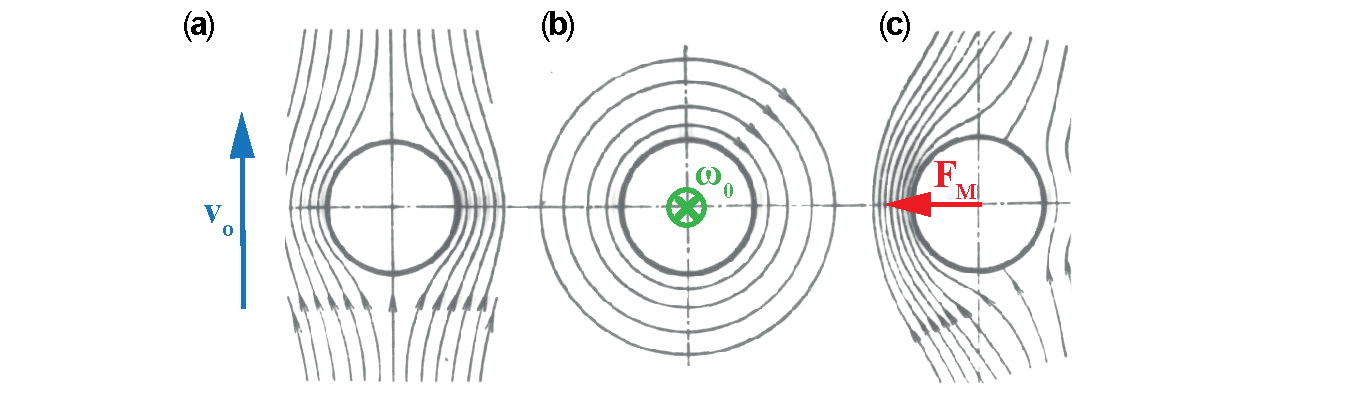
\includegraphics[width=\textwidth]{MagnusEffekt01.pdf}
    \caption[Laminare Str�mung um einen rotierenden Zylinder.]
    {Laminare Str�mung um einen rotierenden Zylinder. \fa Nichtrotierender Zylinder \fb Str�mung in der Grenzschicht \fc �berlagerung.}
    \label{abb:kontmech_magnus01}
\end{figure}

Wir wollen zun�chst eine einfache Plausibilit�tsableitung der Magnus-Kraft machen, bevor wir diese aus der \NVS{} herleiten.
Wir betrachten dabei einen unendlich ausgedehnten Zylinder der L�nge L ($L \gg R$), der sich in einer Str�mumg mit der Geschwindigkeit $\vec{v}_0$ befindet und mit einer Winkelgeschwindigkeit $\vec{\omega}_0$ rotiert.
Die resultierenden Relativgeschwindigkeiten der Fluidstr�mung bez�glich des rotierenden Zylinders ergeben sich dann nach \figref{kontmech_magnus01}\,c folgenderma�en:
\begin{align}
\begin{split}
  \text{linke Seite}:~~~ &\vec{v}_\text{L} = \vec{v}_0 + \vec{\omega}_0 \times \vec{r}~~~~\text{\bzw}\\
  \text{rechte Seite}:~~~&\vec{v}_\text{R} = \vec{v}_0 - \vec{\omega}_0 \times \vec{r}\,.
\end{split}  \label{eq:kontmech_magnus01}
\end{align}

�ber die Bernoulli-Gleichung erhalten wir die Druckdifferenz zwischen beiden Seiten:
\begin{align}
\begin{split}
\Delta p  &= p_\text{R}-p_\text{L} = \frac{\varrho}{2} \lk \vec{v}_\text{L}{}^2 -\vec{v}_\text{R}{}^2 \rk = 2\,\varrho\,\vec{r} \cdot \lk \vec{v}_0  \times \vec{\omega}_0 \rk \,.
\end{split}  \label{eq:kontmech_magnus02}
\end{align}
Daraus ergibt sich eine differentielle Kraft auf ein Oberfl�chenelement nach \figref{kontmech_magnus02} zu:
\begin{align}
\D \vec{F}_\text{M}  &=  2\,\varrho\,\lek \vec{r} \cdot \lk \vec{v}_0  \times \vec{\omega}_0 \rk \rek\, \D \vec{A}\,.
\label{eq:kontmech_magnus02a}
\end{align}
Das differentielle Oberfl�chenelement ist gegeben durch $\D \vec{A} = \vec{r} L\,\D \theta$, wobei wir bereits �ber die Zylinderl�nge $L$ integriert haben.
\begin{align}
\begin{split}
 \D \vec{F}_\text{M}  &=  2\,\varrho\,L \lek R \left| \vec{v}_0  \times \vec{\omega}_0 \right| \cos\theta \rek  \vec{r}\, \D \theta\,.
\end{split}  \label{eq:kontmech_magnus03}
\end{align}

\begin{figure}
    \centering
    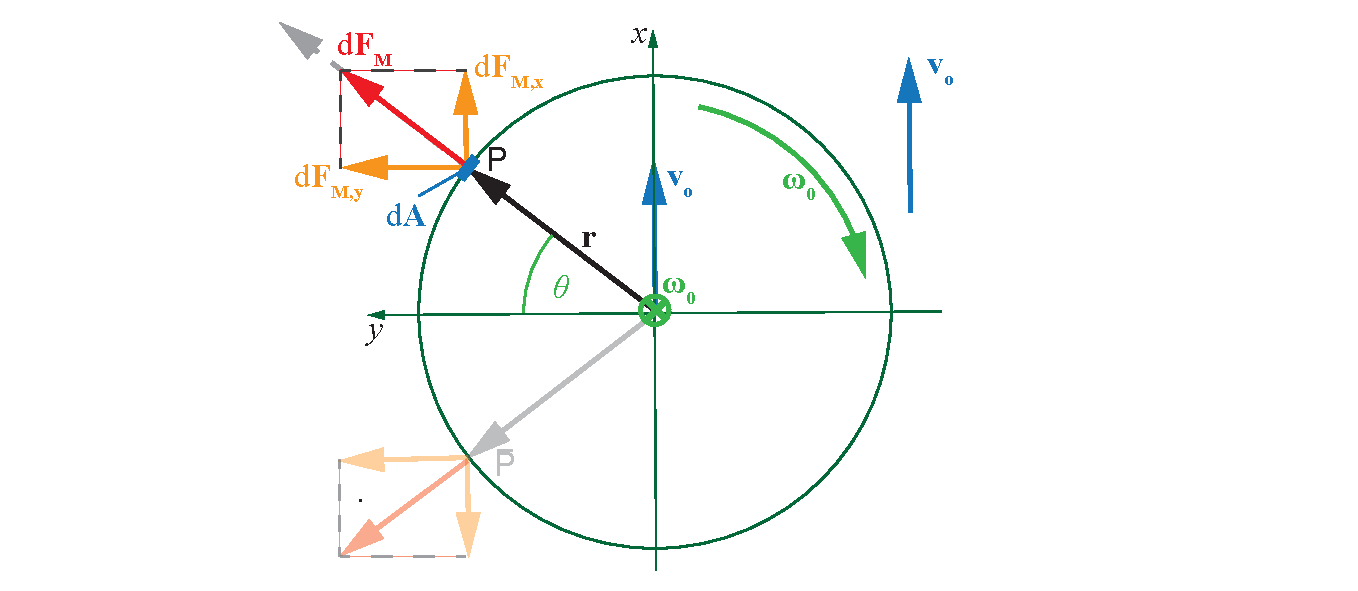
\includegraphics[width=\textwidth]{MagnusEffekt02.pdf}
    \caption[Kraftwirkung auf einen umstr�mten Kreiszylinder.]
    {Kraftwirkung auf einen umstr�mten Kreiszylinder.}
    \label{abb:kontmech_magnus02}
\end{figure}

Das Kraftelement $\D \vec{F}_\text{M}$ wirkt somit in Richtung des Radiusvektors. Wir nutzen jetzt die Symmetrie aus und sehen, dass wir jeweils einen zu $\mathrm{P}$ symmetrischen Punkt $\bar{\mathrm{P}}$ finden, der die gleiche $\D F_{\text{M},y}$-Komponente des Kraftelements hat, deren $\D F_{\text{M},x}$-Komponenten sich aber kompensieren, so dass wir die Integration �ber die gesamte Oberfl�che vereinfachen k�nnen zu:
\begin{align}
\begin{split}
 \vec{F}_\text{M}  & = 4\, \varrho\,L\,R^2\,\left|\vec{v}_0  \times \vec{\omega}_0 \right| \int\limits_{0}^{\pi} \cos^2\theta \,\,\D \theta \, \veceY  = 4\, \varrho\,L\,R^2\,\left|\vec{v}_0  \times \vec{\omega}_0 \right| \,\frac{\pi}2{} \, \veceY \\
                   & = 2\,\pi\,\varrho\,L\,R^2\,\left|\vec{v}_0  \times \vec{\omega}_0 \right| \, \veceY = 2\,\pi\,\varrho\,L\,R^2\, \lk \vec{v}_0  \times \vec{\omega}_0 \rk  \,
\end{split}  \label{eq:kontmech_magnus04}
\end{align}

Auf den Kreiszylinder wirkt also eine senkrecht zur Str�mung gerichtete Kraft, die durch die Zylinderrotation verursacht wird. Dieses Ergebnis findet Anwendung bei Flettner-Rotoren (Rotor-Segelschiffe).\\
Bei optimalen Windverh�ltnissen von \ca $\SI{20}{\metre\per\second}$ quer bis leicht von hinten zur Fahrtrichtung kann der Rotor eine Leistung von etwa 2 MW und mehr erbringen, wobei er mit bis zu 180 Umdrehungen pro Minute rotiert. Die erzeugte Leistung �bersteigt damit die verbrauchte elektrische Leistung von 50 kW des Elektromotors, der das ca 30 Meter hohe Rotorsegel antreibt, um ein Vielfaches. (Siehe \mscr{} \mlkontmechref{FlettnerRotoren.m}.)

Mit dem behandelten Problem des umstr�mten Kreiszylinders haben wir auch den Weg zur Beherrschung des Problems einer umstr�mten Flugzeugtragfl�che bereitet, deren Profil durch eine Abbildung aus dem Kreiszylinderprofil gewonnen werden kann. Bei einer exakten Behandlung eines Flugzeugfl�gels muss man nat�rlich die endliche L�nge des Tragfl�gels ber�cksichtigen, was eine deutliche komplexere 3-dimensionale Aufgabenstellung darstellt.\\
Der Magnus-Effekt spielt auch eine gro�e Rolle bei vielen Ballspielen (Fu�ball, Golf). Hier muss bei der mathematisch-physikalischen Behandlung ebenfalls die endliche Ausdehnung des Ball \bzw der Kugel ber�cksichtigt werden. 
Ebenso sei daraufhin gewiesen, dass wir bei der Herleitung von einer laminaren Str�mung ausgegangen sind, \dh die Betrachtungen gelten nur f�r kleine Reynolds-Zahlen. Bei gr��eren Reynolds-Zahlen treten Verwirbelungen auf, die zu zus�tzlichen Effekten f�hren. Wir werden uns mit solchen Effekten bei der Behandlung des Fliegens als auch bei Untersuchungn zum Ballsport im Band III dieser Reihe intensiver besch�ftigen und dort auch eine allgemeinere Ableitung f�r die Berechnung des Magnus-Effekts geben.

\end{sol} 
\textcolor{blue} {$\rightarrow$ zur} \probref{kontmech_magnus}.\\
\noindent\rule[1ex]{\textwidth}{0.5pt}  \newpage  \clearpage

%-----------------------------------------------------------------------------------------------------------

\begin{sol}{prob:kontmech_SchiffKanal}\label{lsg:kontmech_SchiffKanal} %�bung6
\textbf{Kr�fte auf ein Schiff in einem Kanal}\\ \\

Da Wasser in guter N�herung inkompressibel ist und der Fluss f�r jedes
Zeitintervall $\D t$ an allen Stellen des Schiffes konstant sein muss, k�nnen
wir die Flie�geschwindigkeit aus der verf�gbaren Querschnittsfl�che berechnen.
Die Flie�geschwindigkeit an der Stelle $x$ entlang des Schiffs verh�lt sich
also mit der dort verf�gbaren Fl�che
\begin{align}
  \varrho_\mathrm{W} v(x_1) A(x_1) &= \varrho_\mathrm{W} v(x_2) A(x_2) \notag \\
  \frac{v(x_2)}{v(x_1)} &= \frac{A(x_1)}{A(x_2)} \; , \notag \\
  \frac{v(x)}{v(0)} &= \frac{A(0)}{A(x_2)} \; , \notag \\
  v(x) &= v(0) \, \frac{A(0)}{A(x_2)} \; .
         \label{eq:kontmech_SchiffGeschwindigkeiten}
\end{align}
Als Bezugspunkt nehmen wir das Wasser direkt vor dem Bug des Schiffs. Dort
haben wir (von oben gesehen) auf der linken Seite (vgl.
\figref{kontmech_SchiffKanalAbmessungen}) die Fl�che
\begin{subequations}
  \begin{align}
    A_\mathrm{l}(0) &= a_1 (c_1+c_2) \label{eq:kontmech_SchiffFlaeche1} \\
    \intertext{und auf der rechten Seite}
    A_\mathrm{r}(0) &= a_2 (c_1+c_2) \label{eq:kontmech_SchiffFlaeche2}
  \end{align}
\end{subequations}

Die Querschnittsfl�che, durch die das Wasser str�men kann, h�ngt vom Abstand
$d$ zwischen der Schiffswand und der Wand des Kanals ab. Der Abstand $d$ ist
selbst wieder vom Abstand $x$ vom Bug und der H�he $z$ �ber dem Kiel abh�ngig.
Betrachten wir zun�chst die (von oben gesehen) linke Seite und dort die
Koordinate $y$, so finden wir anhand von
\figref{kontmech_SchiffKanalAbmessungen}
\begin{equation*}
  d_\mathrm{l}(x,z) = a_1 - \frac{B(x,z)}{2} \; .
\end{equation*}
Die von der H�he �ber dem Kliel und der Entfernung vom Bug abh�ngige Breite
$B(x,z)$ des Schiffs ergibt sich nach der Abbildung zu
\begin{equation*}
  B(x,z) = \begin{cases}
    \frac{B(x)}{c_2} \, z & \text{f�r } z < c_2 \; , \\
    B(x) & \text{f�r } c_2 < z \le c_1 + c_2 \; , \\
  \end{cases}
\end{equation*}
wobei im oberen Teil des Schiffes, wo es seine maximale Breite erreicht, gilt
\begin{equation*}
  B(x) = \begin{cases}
    \frac{b}{l_2}\, x & \text{f�r } x \le l_2 \; , \\
    b & \text{f�r } l_2 < x  \le l_1 + l_2 \; .
  \end{cases} 
\end{equation*}

Insgesamt erh�lt man
\begin{equation*}
  B(x,z) = \begin{cases}
    \frac{b}{l_2\,c_2}\, x \, z & \text{f�r } x \le l_2
    \text{ und } z < c_2 \; , \\
    \frac{b}{l_2}\, x  & \text{f�r } x \le l_2 \text{ und }
    c_2 < z \le c_1 + c_2 \; , \\
    \frac{b}{c_2}\, z  & \text{f�r } l_2 < x  \le l_1 + l_2
    \text{ und } z < c_2 \; , \\
    b & \text{f�r } l_2 < x  \le l_1 + l_2 \text{ und } c_2 < z \le c_1
    + c_2 \; .
  \end{cases} 
\end{equation*}
und damit auf der linken Seite
\begin{equation*}
  d_\mathrm{l}(x,z) = \begin{cases}
    a_1 - \frac{b}{2\,l_2\,c_2}\, x \, z & \text{f�r } x \le l_2
    \text{ und } z < c_2 \; , \\
    a_1 - \frac{b}{2\,l_2}\, x  & \text{f�r } x \le l_2 \text{ und }
    c_2 < z \le c_1 + c_2 \; , \\
    a_1 - \frac{b}{2\,c_2}\, z  & \text{f�r } l_2 < x  \le l_1 + l_2
    \text{ und } z < c_2 \; , \\
    a_1 - \frac{b}{2} & \text{f�r } l_2 < x  \le l_1 + l_2
    \text{ und } c_2 < z \le c_1 + c_2 \; .
  \end{cases} 
\end{equation*}
sowie analog auf der rechten Seite  
\begin{equation*}
  d_\mathrm{r}(x,z) = \begin{cases}
    a_2 - \frac{b}{2\,l_2\,c_2}\, x \, z & \text{f�r } x \le l_2 \text{ und }
    z < c_2 \; , \\
    a_2 - \frac{b}{2\,l_2}\, x  & \text{f�r } x \le l_2 \text{ und }
    c_2 < z \le c_1 + c_2 \; , \\
    a_2 - \frac{b}{2\,c_2}\, z  & \text{f�r } l_2 < x  \le l_1 + l_2
    \text{ und } z < c_2 \; , \\
    a_2 - \frac{b}{2} & \text{f�r } l_2 < x  \le l_1 + l_2 \text{ und }
    c_2 < z \le c_1 + c_2 \; .
  \end{cases} 
\end{equation*}

Dies k�nnen wir nun nutzen, um die Querschnittsfl�che zu berechnen. Wir
erhalten f�r $x < l_2$
\begin{multline*}
  A_\mathrm{l}(x) = \int_{0}^{c_1 + c_2} d_\mathrm{l}(x,z) \, \D z
  = \int_{0}^{c_2} \lk a_1 - \frac{b}{2\,l_2\,c_2}\, x \, z \rk \D z
  + \int_{c_2}^{c_1 + c_2}  \lk a_1 - \frac{b}{2\,l_2}\, x \rk \D z \\
  = a_1 \, c_2 -  \frac{b\,c_2}{4\,l_2} \, x
  + \lk a_1 - \frac{b}{2\,l_2}\, x \rk c_1
  = a_1 \lk c_1 + c_2 \rk - \frac{b \lk 2 c_1 + c_2 \rk}{4\,l_2} \, x 
\end{multline*}
und im Fall $l_2 < x \le l_1 + l_2$
\begin{multline*}
  A_\mathrm{l} = \int_{0}^{c_1 + c_2} d_\mathrm{l}(x,z) \, \D z
  = \int_{0}^{c_2} \lk a_1 - \frac{b}{2\,c_2}\, z \rk \D z
  + \int_{c_2}^{c_1 + c_2}  \lk a_1 - \frac{b}{2} \rk \D z \\
  = a_1 \, c_2 -  \frac{b\,c_2}{4} 
  + \lk a_1 - \frac{b}{2} \rk c_1
  = a_1 \lk c_1 + c_2 \rk - \frac{b \lk 2 c_1 + c_2 \rk}{4} 
\end{multline*}
Dies l�sst sich zusammenfassen zu
\begin{equation*}
  A_\mathrm{l}(x) = \begin{cases}
    a_1 \lk c_1 + c_2 \rk - \frac{b \lk 2 c_1 + c_2 \rk}{4\,l_2} \, x
    & \text{f�r } x < l_2 \; , \\
    a_1 \lk c_1 + c_2 \rk - \frac{b \lk 2 c_1 + c_2 \rk}{4}
    & \text{f�r } l_2 < x \le l_1 + l_2 \; .
  \end{cases}
\end{equation*}
und f�r die rechte Seite vollkommen analog berechnen zu
\begin{equation*}
  A_\mathrm{r}(x) = \begin{cases}
    a_2 \lk c_1 + c_2 \rk - \frac{b \lk 2 c_1 + c_2 \rk}{4\,l_2} \, x
    & \text{f�r } x < l_2 \; , \\
    a_2 \lk c_1 + c_2 \rk - \frac{b \lk 2 c_1 + c_2 \rk}{4}
    & \text{f�r } l_2 < x \le l_1 + l_2 \; .
  \end{cases}
\end{equation*}

Die bisher durchgef�hrten Zwischenrechnungen erm�glichen uns nun, die
Flie�gechwindigkeit des Wassers relativ zum Schiff abh�ngig vom Ort $x$
zu bestimmen. Zusammen mit \eqref{eq:kontmech_SchiffGeschwindigkeiten},
den Fl�chen $A_\mathrm{l}(0)$ und $A_\mathrm{r}(0)$ aus den Gleichungen
\eqref{eq:kontmech_SchiffFlaeche1} und \eqref{eq:kontmech_SchiffFlaeche1}
sowie $v(0) = v_0$ erhalten wir
\begin{align}
  v_\mathrm{l}(x) &= \begin{cases} v_0 \, \frac{a_1 \lk c_1 + c_2 \rk}{a_1
      \lk c_1 + c_2 \rk - \frac{b \lk 2 c_1 + c_2 \rk}{4\,l_2} \, x}
    & \text{f�r } x < l_2 \; , \\
    v_0 \, \frac{a_1 \lk c_1 + c_2 \rk}{a_1 \lk c_1 + c_2 \rk - \frac{b
        \lk 2 c_1 + c_2 \rk}{4}}
    & \text{f�r } l_2 < x \le l_1 + l_2 
  \end{cases} \\
  \intertext{und}
  v_\mathrm{r}(x) &= \begin{cases} v_0 \, \frac{a_2 \lk c_1 + c_2 \rk}{a_2
      \lk c_1 + c_2 \rk - \frac{b \lk 2 c_1 + c_2 \rk}{4\,l_2} \, x}
    & \text{f�r } x < l_2 \; , \\
    v_0 \, \frac{a_2 \lk c_1 + c_2 \rk}{a_2 \lk c_1 + c_2 \rk - \frac{b
        \lk 2 c_1 + c_2 \rk}{4}}
    & \text{f�r } l_2 < x \le l_1 + l_2 \; . 
  \end{cases} 
\end{align}

Sei $p_0$ der Druck im Wasser, das relativ zum Schiff die Flie�geschwindigkeit
$v_0$ habe. Dann l�sst sich mit der Bernoulli-Gleichung
\eqref{eq:kontmech_BernoulliGl} der Druck auf die Seitenw�nde des Schiffs
ermitteln. Wir finden auf der linken Seite
\begin{equation*}
  \frac{1}{2} \varrho \, v_l(x)^2 + p_l(x) = \frac{1}{2} \varrho \, v_0^2 + p_0
\end{equation*}
oder 
\begin{align*}
  p_l(x) &= p_0 + \frac{1}{2} \varrho \lk v_0^2 -  v_l(x)^2 \rk \\
         &= p_0 + \frac{1}{2} \varrho v_0^2 \begin{cases}
           1 - \lk \frac{a_1 \lk c_1 + c_2 \rk}{a_1\lk c_1 + c_2 \rk
             - \frac{b \lk 2 c_1 + c_2 \rk}{4\,l_2} \, x} \rk^2 
           & \text{f�r } x < l_2 \; , \\
         1 - \lk \frac{a_1 \lk c_1 + c_2 \rk}{a_1 \lk c_1 + c_2 \rk - \frac{b
             \lk 2 c_1 + c_2 \rk}{4}} \rk^2
         & \text{f�r } l_2 < x \le l_1 + l_2 \; .
         \end{cases}
\end{align*}
Analog findet man auf der rechten Seite
\begin{align*}
  p_r(x) &= p_0 + \frac{1}{2} \varrho \lk v_0^2 -  v_r(x)^2 \rk \\
         &= p_0 + \frac{1}{2} \varrho v_0^2 \begin{cases}
           1 - \lk \frac{a_2 \lk c_1 + c_2 \rk}{a_2\lk c_1 + c_2 \rk
             - \frac{b \lk 2 c_1 + c_2 \rk}{4\,l_2} \, x} \rk^2 
           & \text{f�r } x < l_2 \; , \\
         1 - \lk \frac{a_2 \lk c_1 + c_2 \rk}{a_2 \lk c_1 + c_2 \rk - \frac{b
             \lk 2 c_1 + c_2 \rk}{4}} \rk^2
         & \text{f�r } l_2 < x \le l_1 + l_2 \; .
         \end{cases}
\end{align*}
F�r die resultierende Kraft und das resultierende Moment auf das Schiff
reicht es, in den folgenden Schritten aufgrund der Symmetrie des Schiffs
von der Druckdifferenz auf beiden Seiten auszugehen. Nach
\figref{kontmech_SchiffKanalAbmessungen} erwarten wir einen gr��eren
Druck auf der linken Seite, da dort die Querschnittsfl�che gr��er und somit
die Flie�geschwindigkeit kleiner ist, und somit eine effektive Kraftwirkung
nach rechts. Diese wird von der Durckdifferenz
\begin{align}
  \Delta p &= p_l(x) - p_r(x) \\
           &= \frac{1}{2} \varrho v_0^2 \begin{cases}
             \lk \frac{a_1 \lk c_1 + c_2 \rk}{a_1\lk c_1 + c_2 \rk
               - \frac{b \lk 2 c_1 + c_2 \rk}{4\,l_2} \, x} \rk^2
             - \lk \frac{a_2 \lk c_1 + c_2 \rk}{a_2\lk c_1 + c_2 \rk
               - \frac{b \lk 2 c_1 + c_2 \rk}{4\,l_2} \, x} \rk^2 
             & \text{f�r } x < l_2 \; , \\
             \lk \frac{a_1 \lk c_1 + c_2 \rk}{a_1 \lk c_1 + c_2 \rk - \frac{b
                 \lk 2 c_1 + c_2 \rk}{4}} \rk^2
             - \lk \frac{a_2 \lk c_1 + c_2 \rk}{a_2 \lk c_1 + c_2 \rk - \frac{b
                 \lk 2 c_1 + c_2 \rk}{4}} \rk^2
             & \text{f�r } l_2 < x \le l_1 + l_2
           \end{cases}
               \label{eq:kontmech_SchiffKanalDruckdiff}
\end{align}
bewirkt.

Die Kraft und das Drehmoment sollen auf den Schwerpunkt des Schiffes bezogen
werden. Da wir uns nur an der Bewegung in der $x$-$y$-Ebene interessiert
sind, ben�tigen wir auch den Schwerpunkt nur in dieser. Aus Symmeriegr�nden
erkennt man sofort, dass $y_\mathrm{S} = 0$. F�r die $x$-Koordinate m�ssen
wir jedoch die Form des Bugs ber�cksichtigen. Wir berechnen unter
Ber�cksichtigung der homegenen Massendichte
\begin{subequations}
  \allowdisplaybreaks
  \begin{multline}
    x_\mathrm{S} = \frac{1}{V} \int_{0}^{l_1+l_2}\D x \, \int_{0}^{c_1+c_2} \D z \,
    \int_{-B(x,z)/2}^{B(x,z)/2} \D y \, x
    = \frac{1}{V} \int_{0}^{l_1+l_2}\D x \, \int_{0}^{c_1+c_2} \D z \, x \,
    B(x,z) \\
    = \frac{1}{V} \int_{0}^{l_1+l_2}\D x \left \{ \int_{0}^{c_2} \D z \, x \,
      \frac{B(x)}{c_2} \, z + \int_{c_2}^{c_1 + c_2} \D z \, x \, B(x) \right \}
    = \frac{1}{V} \int_{0}^{l_1+l_2}\D x \left \{ x \, \frac{c_2}{2} \, B(x)
      + x \, c_1 \, B(x) \right \} \\
    = \frac{1}{V} \int_{0}^{l_1+l_2}\D x \, x \lk \frac{c_2}{2} +c_1 \rk B(x)
    = \frac{1}{V} \lk \frac{c_2}{2} +c_1 \rk  \left \{ \int_{0}^{l_2}\D x
      \, \frac{b}{l_2}\, x^2 +  \int_{l_2}^{l_1 + l_2}\D x \, b \, x
    \right \} \\
    = \frac{1}{V} \lk \frac{c_2}{2} +c_1 \rk  \left \{ \frac{b\,l_2^2}{3}
      + \frac{b\,\lk l_1 + l_2 \rk^2}{2} - \frac{b\, l_2^2}{2}\right \}
    = \frac{1}{V} \lk \frac{c_2}{2} +c_1 \rk  b \left \{ \frac{\lk l_1 + l_2
        \rk^2}{2} - \frac{l_2^2}{6} \right \}
    \label{eq:kontmech_SchiffSchwerpunkt1}
  \end{multline}
  Mit dem Volumen des Schiffs
  \begin{multline}
    V = \int_{0}^{l_1+l_2}\D x \, \int_{0}^{c_1+c_2} \D z \,
    \int_{-B(x,z)/2}^{B(x,z)/2} \D y 
    = \int_{0}^{l_1+l_2}\D x \lk \frac{c_2}{2} +c_1 \rk B(x) \\
    = \lk \frac{c_2}{2} +c_1 \rk  \left \{ \int_{0}^{l_2}\D x
      \, \frac{b}{l_2}\, x +  \int_{l_2}^{l_1 + l_2}\D x \, b \right \} 
    = \lk \frac{c_2}{2} +c_1 \rk  \left \{ \frac{b\,l_2}{2}
      + b\,\lk l_1 + l_2 \rk - b\, l_2 \right \}
    = \lk \frac{c_2}{2} +c_1 \rk  b \lk l_1 + \frac{l_2}{2} \rk
    \label{eq:kontmech_SchiffVolumen}
  \end{multline}
  f�hrt das schlie�lich auf
  \begin{equation}
    x_\mathrm{S} = \frac{\frac{\lk l_1 + l_2 \rk^2}{2} - \frac{l_2^2}{6}}
    {l_1 + \frac{l_2}{2}} = \frac{3 \lk l_1 + l_2 \rk^2 - l_2^2}
    {6 \, l_1 + 3 \, l_2}
    = \frac{3 l_1^2 + 6 l_1 l_2 +2 l_2^2}{6 \, l_1 + 3 \, l_2}
    \; .
    \label{eq:kontmech_SchiffSchwerpunkt2}
  \end{equation}
\end{subequations}

Wir berechnen zun�chst die Kraft auf den Schwerpunkt. Diese hat zwei
Komponenten. Auf den Bug wirkt ein kleinerer Druck als auf das Heck. Das hat
eine Kraft in negativer $x$-Richtung zur Folge, die uns hier jedoch nicht
interessiert, da sie mit einer Kursabweichung des Schiffst nichts zu tun
hat und in dieser Richtung weitere Komponenten wie der Antrieb oder die
Reibung �berwiegen. Jedoch gibt es auch eine $y$-Komponente. Diese ergibt sich
aus dem Druckunterschied bezogen auf die projizierte Fl�che der Schiffswand
auf die $x$-$z$-Ebene, wobei die projizierte H�he  $c_1 + c_2$ betr�gt. Man
erh�lt
{ \allowdisplaybreaks
  \begin{multline}
    F_y = (c_1+c_2) \int_0^{l_1+ l_2} \Delta p(x)\,\D x \\
    = \frac{1}{2} \varrho v_0^2 \, (c_1+c_2) \int_0^{l_2}
    \left \{ \lk \frac{a_1 \lk c_1 + c_2 \rk}{a_1\lk c_1 + c_2 \rk
        - \frac{b \lk 2 c_1 + c_2 \rk}{4\,l_2} \, x} \rk^2
      - \lk \frac{a_2 \lk c_1 + c_2 \rk}{a_2\lk c_1 + c_2 \rk
        - \frac{b \lk 2 c_1 + c_2 \rk}{4\,l_2} \, x} \rk^2 \right \} \,\D x \\
    + \frac{1}{2} \varrho v_0^2 \, (c_1+c_2) \, l_1 \left \{
      \lk \frac{a_1 \lk c_1 + c_2 \rk}{a_1 \lk c_1 + c_2 \rk - \frac{b
          \lk 2 c_1 + c_2 \rk}{4}} \rk^2
      - \lk \frac{a_2 \lk c_1 + c_2 \rk}{a_2 \lk c_1 + c_2 \rk - \frac{b
          \lk 2 c_1 + c_2 \rk}{4}} \rk^2 \right \}  \\
    = \frac{1}{2} \varrho v_0^2 \, (c_1+c_2) \, \frac{4\,l_2}{b \lk 2 c_1
      + c_2 \rk}
    \left . \left \{ \frac{a_1^2 \lk c_1 + c_2 \rk^2}{a_1\lk c_1 + c_2 \rk
          - \frac{b \lk 2 c_1 + c_2 \rk}{4\,l_2} \, x} 
        - \frac{a_2^2 \lk c_1 + c_2 \rk^2}{a_2\lk c_1 + c_2 \rk
          - \frac{b \lk 2 c_1 + c_2 \rk}{4\,l_2} \, x}  \right \}
    \right |_{0}^{l_2} \\
    + \frac{1}{2} \varrho v_0^2 \, (c_1+c_2) \, l_1 \left \{
      \lk \frac{a_1 \lk c_1 + c_2 \rk}{a_1 \lk c_1 + c_2 \rk - \frac{b
          \lk 2 c_1 + c_2 \rk}{4}} \rk^2
      - \lk \frac{a_2 \lk c_1 + c_2 \rk}{a_2 \lk c_1 + c_2 \rk - \frac{b
          \lk 2 c_1 + c_2 \rk}{4}} \rk^2 \right \}  \\
    = \frac{1}{2} \varrho v_0^2 \, \frac{4\,l_2\lk c_1 + c_2\rk}{b\lk 2c_1
      + c_2 \rk}
    \Bigg \{ \frac{a_1^2 \lk c_1 + c_2 \rk^2}{a_1\lk c_1 + c_2 \rk
      - \frac{b \lk 2 c_1 + c_2 \rk}{4}}
    - a_1 \lk c_1 + c_2 \rk 
    - \frac{a_2^2 \lk c_1 + c_2 \rk^2}{a_2\lk c_1 + c_2 \rk
      - \frac{b \lk 2 c_1 + c_2 \rk}{4}} 
    + a_2 \, \lk c_1 + c_2 \rk  \Bigg \} \\
    + \frac{1}{2} \varrho v_0^2 \, (c_1+c_2) \, l_1 \left \{
      \lk \frac{a_1 \lk c_1 + c_2 \rk}{a_1 \lk c_1 + c_2 \rk - \frac{b
          \lk 2 c_1 + c_2 \rk}{4}} \rk^2
      - \lk \frac{a_2 \lk c_1 + c_2 \rk}{a_2 \lk c_1 + c_2 \rk - \frac{b
          \lk 2 c_1 + c_2 \rk}{4}} \rk^2 \right \}  \; . \\
  \end{multline}
}

W�hrend f�r die Kraft schnell einsichtig war, dass die auf die $x$-$z$-Ebene
projizierte Fl�che herangezogen werden kann, um die effektive Kraft zu
berechnen, ist eine �hnliche Vereinfachung f�r das Drehmoment nicht so
schnell zu erkennen. Doch auch hier k�nnen wir einen recht einfachen Ausdruck
finden, der sich auf die Druckdifferenz zur�ckf�hren l�sst. Um das zu erkennen
betrachten wir \figref{kontmech_SchiffKanalKraefte}.

\begin{figure}
  \centering
  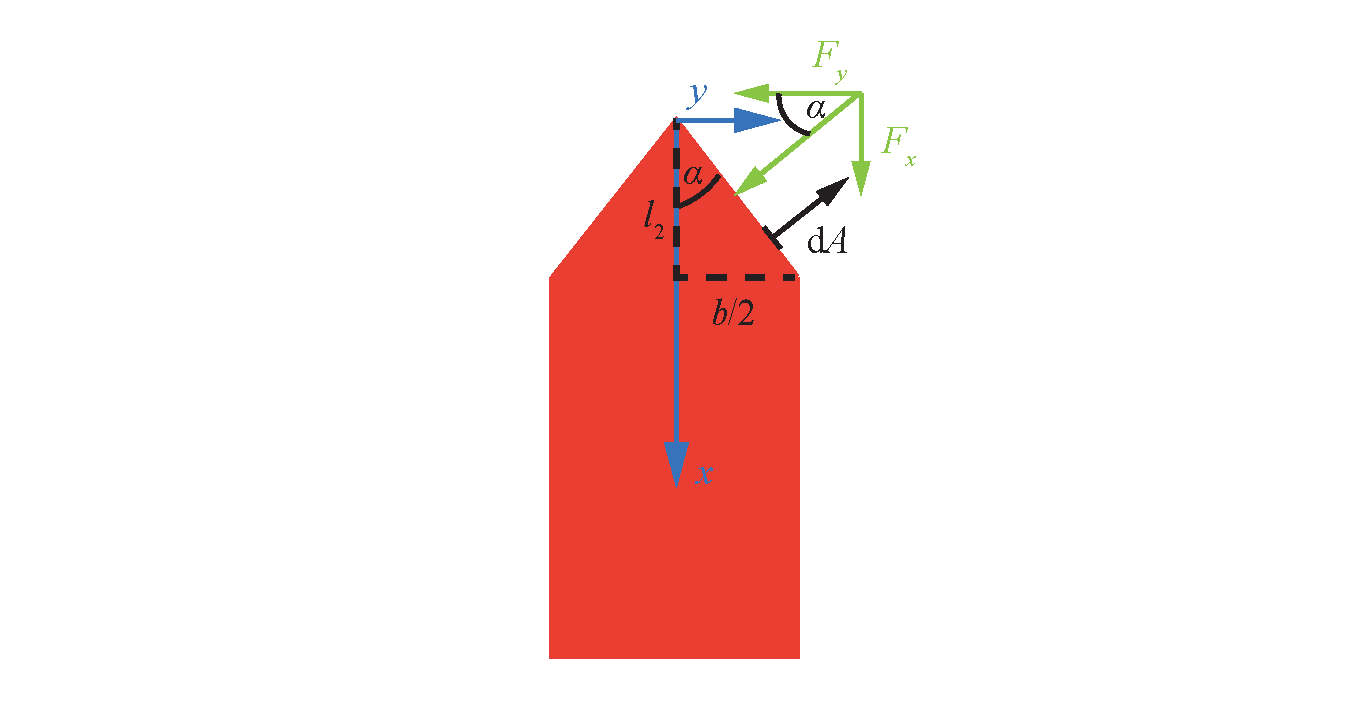
\includegraphics[width=\textwidth]{SchiffKanalKraefte}
  \caption[Kr�fte auf ein Schiff im Kanal]
  {Kr�fte auf eine Schiff im Kanal, wie sie durch den Wasserdruck
    verursacht werden.}
  \label{abb:kontmech_SchiffKanalKraefte}
\end{figure}

Da wir nur an Drehungen um die $z$-Achse interessiert sind, m�ssen wir
keine Kraftkomponenten in $z$-Richtung beachten, denn diese k�nnten kein
solches Drehmoment bewirken. In jeder H�he interessieren wir uns also nur
vom Abstand des Angriffspunkts einer Kraft von der $z$-Achse um den
Schwerpunkt, den wir entsprechend auf der linken und rechten Seite des
Bugs mit 
\begin{equation}
  \vec{r}_r = \begin{pmatrix} x-x_\mathrm{S} \\ y \\ 0 \end{pmatrix} \; , \qquad
  \vec{r}_l = \begin{pmatrix} x-x_\mathrm{S} \\ -y \\ 0 \end{pmatrix} 
\end{equation}
angeben k�nnen. F�r Kr�fte, die auf beiden Seiten jeweils auf das
Fl�chenelement $\D A$ wirken, finden wir
\begin{equation}
  \D \vec{F}_r = \begin{pmatrix} p_r \,\D A\, \sin\alpha \\
    -p_r \, \D A \, \cos\alpha \\ 0 \end{pmatrix} \; , \qquad
  \D \vec{F}_l = \begin{pmatrix} p_l \,\D A\, \sin\alpha \\
    p_l \, \D A \, \cos\alpha \\ 0 \end{pmatrix} \; .
\end{equation}
Um unteren schr�gen Teil des Rumpfes wirkt die Kraft durch den Druck
nat�rlich nicht nur in der $x$-$y$-Ebene. Da wir sp�ter jedoch wieder
�ber die H�he $c_1$ integrieren, um das gesamte Drehmoment zu erhalten,
und nicht �ber die schr�ge Fl�che ber�cksichtigen wir automatisch nur
die relevante Kraftkomponente. Die $z$-Komponente der Kraft ist, wie oben
beschrieben, f�r uns nicht relevant und wird hier zur �bersichtlichkeit
in der Rechnung nicht angegeben.

Das Drehmoment berechnet sich dann zu
\begin{equation}
  \D \vec{M} = \vec{r}_r \times \vec{F}_r + \vec{r}_l \times \vec{F}_l 
  = \begin{pmatrix} x-x_\mathrm{S} \\ y \\ 0 \end{pmatrix}
  \times \begin{pmatrix} p_r \,\D A\, \sin\alpha \\
    -p_r \, \D A \, \cos\alpha \\ 0 \end{pmatrix}
  + \begin{pmatrix} x-x_\mathrm{S} \\ -y \\ 0 \end{pmatrix}
  \times \begin{pmatrix} p_l \,\D A\, \sin\alpha \\
    p_l \, \D A \, \cos\alpha \\ 0 \end{pmatrix}
\end{equation}
mit der f�r uns relevanten $z$-Komponente
\begin{multline}
  \D M_z = - (x-x_\mathrm{S}) p_r \, \D A\, \cos\alpha - y\, p_r \, \D A \,
  \sin\alpha
  + (x-x_\mathrm{S}) p_l \, \D A\, \cos\alpha - y\, p_l \, \D A \, \sin\alpha \\
  = -(x \, \cos\alpha + y\, \sin\alpha) p_r \,\D A + x_\mathrm{S} \, \cos\alpha
  \, p_r \, \D A 
  + (x \, \cos\alpha + y\, \sin\alpha) p_l \,\D A - x_\mathrm{S} \, \cos\alpha
  \, p_l \, \D A \\
  = (x \, \cos\alpha + y\, \sin\alpha) \Delta p(x) \,\D A
  - x_\mathrm{S} \, \cos\alpha \, \Delta p(x) \, \D A \; .
\end{multline}
Hier erkennen wir bereits, dass erneut nur die Druckdifferenz entscheidend
ist. Die Ausdr�cke lassen sich jedoch weiter vereinfachen. Wir ber�cksichtigen,
dass nach \figref{kontmech_SchiffKanalKraefte}
\begin{equation}
  \tan \alpha = \frac{y}{x} \qquad \text{bzw.} \qquad
  y(x) = \tan\alpha\, x \; .
\end{equation}
Damit erhalten wir
\begin{equation}
  \D M_z = \lk x \, \cos\alpha + x\, \frac{\sin^2\alpha}{\cos\alpha} \rk
  \Delta p(x) \,\D A - x_\mathrm{S} \, \cos\alpha \, \Delta p(x) \, \D A 
  = \frac{x}{\cos\alpha}\, \Delta p(x) \,\D A
  - x_\mathrm{S} \, \cos\alpha \, \Delta p(x) \, \D A \; .
\end{equation}
Wenn wir nun noch nach \figref{kontmech_SchiffKanalKraefte} ber�cksichtigen,
dass
\begin{equation}
  \D A = \lk c_1 + c_2 \rk \frac{\D x}{\cos\alpha} \; ,
\end{equation}
dann f�hrt das auf
\begin{equation}
  \D M_z = \frac{x}{\cos^2\alpha}\, \Delta p(x) \, \lk c_1 + c_2 \rk \, \D x
  - x_\mathrm{S} \, \Delta p(x) \, \lk c_1 + c_2 \rk \, \D x \; .
\end{equation}
Schlie�lich dr�cken wir den Winkel $\alpha$ durch bekannte Ma�e des Schiffs
aus,
\begin{equation*}
  \cos \alpha = \frac{l_2}{\sqrt{l_2^2 + (b/2)^2}} \;, \qquad \text{also}
  \qquad \frac{1}{\cos^2\alpha} = \frac{l_2^2 + b^2/4}{l_2^2}
  = 1 + \frac{b^2}{4 l_2^2} \; ,
\end{equation*}
und erhalten daraus
\begin{equation}
  \D M_z = x \, \Delta p(x) \, \lk 1 + \frac{b^2}{4 l_2^2} \rk 
  \lk c_1 + c_2 \rk \, \D x
  - x_\mathrm{S} \, \Delta p(x) \, \lk c_1 + c_2 \rk \, \D x \; .
\end{equation}

F�r den Anteil des Bugs erhalten wir damit
{
  \allowdisplaybreaks
  \begin{multline}
    \lk M_1 \rk_z = \int_0^{l_2} \D M_z
    = \lk 1 + \frac{b^2}{4 l_2^2} \rk \lk c_1 + c_2 \rk  \int_0^{l_2} x \,
    \Delta p(x) \, \D x
    - x_\mathrm{S} \, \lk c_1 + c_2 \rk \, \int_0^{l_2} \Delta p(x) \, \D x \\
    % 
    = \frac{1}{2} \varrho v_0^2 \, \lk 1 + \frac{b^2}{4 l_2^2} \rk \lk c_1
    + c_2 \rk  \int_0^{l_2} x \, \left \{ \lk \frac{a_1 \lk c_1 + c_2 \rk}
      {a_1\lk c_1 + c_2 \rk - \frac{b \lk 2 c_1 + c_2 \rk}{4\,l_2} \, x} \rk^2
      - \lk \frac{a_2 \lk c_1 + c_2 \rk}{a_2\lk c_1 + c_2 \rk
        - \frac{b \lk 2 c_1 + c_2 \rk}{4\,l_2} \, x} \rk^2 \right \} \, \D x \\
    - \frac{1}{2} \varrho v_0^2 \, x_\mathrm{S} \lk c_1 + c_2 \rk \, \int_0^{l_2}
    \left \{ \lk \frac{a_1 \lk c_1 + c_2 \rk}{a_1\lk c_1 + c_2 \rk
        - \frac{b \lk 2 c_1 + c_2 \rk}{4\,l_2} \, x} \rk^2
      - \lk \frac{a_2 \lk c_1 + c_2 \rk}{a_2\lk c_1 + c_2 \rk
        - \frac{b \lk 2 c_1 + c_2 \rk}{4\,l_2} \, x} \rk^2 \right \} \,\D x \\
    % 
    = \frac{1}{2} \varrho v_0^2 \, \lk 1 + \frac{b^2}{4 l_2^2} \rk \lk c_1
    + c_2 \rk \, \frac{4\,l_2}{b \lk 2 c_1 + c_2 \rk}
    \left . x \, \left \{ \frac{a_1^2 \lk c_1 + c_2 \rk^2}{a_1\lk c_1 + c_2 \rk
          - \frac{b \lk 2 c_1 + c_2 \rk}{4\,l_2} \, x} 
        - \frac{a_2^2 \lk c_1 + c_2 \rk^2}{a_2\lk c_1 + c_2 \rk
          - \frac{b \lk 2 c_1 + c_2 \rk}{4\,l_2} \, x}  \right \}
    \right |_{0}^{l_2} \\
 - \frac{1}{2} \varrho v_0^2 \, \lk 1 + \frac{b^2}{4 l_2^2} \rk \lk c_1
    + c_2 \rk \, \frac{4\,l_2}{b \lk 2 c_1 + c_2 \rk} \int_0^{l_2} 
    \left \{ \frac{a_1^2 \lk c_1 + c_2 \rk^2}{a_1\lk c_1 + c_2 \rk
        - \frac{b \lk 2 c_1 + c_2 \rk}{4\,l_2} \, x} 
      - \frac{a_2^2 \lk c_1 + c_2 \rk^2}{a_2\lk c_1 + c_2 \rk
        - \frac{b \lk 2 c_1 + c_2 \rk}{4\,l_2} \, x}  \right \} \, \D x \\
    - \frac{1}{2} \varrho v_0^2 \, x_\mathrm{S} \frac{4\,l_2 \lk c_1 + c_2 \rk}
    {b \lk 2c_1 + c_2 \rk}
    \Bigg \{ \frac{a_1^2 \lk c_1 + c_2 \rk^2}{a_1\lk c_1 + c_2 \rk
      - \frac{b \lk 2 c_1 + c_2 \rk}{4}}
    - a_1 \lk c_1 + c_2 \rk 
    - \frac{a_2^2 \lk c_1 + c_2 \rk^2}{a_2\lk c_1 + c_2 \rk
      - \frac{b \lk 2 c_1 + c_2 \rk}{4}} 
    + a_2 \, \lk c_1 + c_2 \rk  \Bigg \} \\
    % 
    = \frac{1}{2} \varrho v_0^2 \, \lk 1 + \frac{b^2}{4 l_2^2} \rk \,
    \frac{4\,l_2^2 \lk c_1 + c_2 \rk}{b \lk 2 c_1 + c_2 \rk}
    \left \{\frac{a_1^2 \lk c_1 + c_2 \rk^2}{a_1\lk c_1 + c_2 \rk
        - \frac{b \lk 2 c_1 + c_2 \rk}{4}} 
      - \frac{a_2^2 \lk c_1 + c_2 \rk^2}{a_2\lk c_1 + c_2 \rk
        - \frac{b \lk 2 c_1 + c_2 \rk}{4}}  \right \} \\
    + \frac{1}{2} \varrho v_0^2 \, \lk 1 + \frac{b^2}{4 l_2^2} \rk \,
    \frac{16\,l_2^2 \lk c_1 + c_2 \rk}{b^2 \lk 2 c_1 + c_2 \rk^2}  
    \Biggl \{ a_1^2 \lk c_1 + c_2 \rk^2 \ln \lk a_1\lk c_1 + c_2 \rk
          - \frac{b \lk 2 c_1 + c_2 \rk}{4\,l_2} \, x \rk \\
        - a_2^2 \lk c_1 + c_2 \rk^2 \ln \lk a_2\lk c_1 + c_2 \rk
          - \frac{b \lk 2 c_1 + c_2 \rk}{4\,l_2} \, x \rk  \Biggr \}
    \Biggr |_{0}^{l_2} \\
    - \frac{1}{2} \varrho v_0^2 \, x_\mathrm{S} \frac{4\,l_2}{b}
    \Bigg \{ \frac{a_1^2 \lk c_1 + c_2 \rk^2}{a_1\lk c_1 + c_2 \rk
      - \frac{b \lk 2 c_1 + c_2 \rk}{4}}
    - a_1 \lk c_1 + c_2 \rk 
    - \frac{a_2^2 \lk c_1 + c_2 \rk^2}{a_2\lk c_1 + c_2 \rk
      - \frac{b \lk 2 c_1 + c_2 \rk}{4}} 
    + a_2 \, \lk c_1 + c_2 \rk  \Bigg \} \\ 
    % 
    = \frac{1}{2} \varrho v_0^2 \, \lk 1 + \frac{b^2}{4 l_2^2} \rk \,
    \frac{4\,l_2^2 \lk c_1 + c_2 \rk}{b \lk 2 c_1 + c_2 \rk}
    \left \{\frac{a_1^2 \lk c_1 + c_2 \rk^2}{a_1\lk c_1 + c_2 \rk
        - \frac{b \lk 2 c_1 + c_2 \rk}{4}} 
      - \frac{a_2^2 \lk c_1 + c_2 \rk^2}{a_2\lk c_1 + c_2 \rk
        - \frac{b \lk 2 c_1 + c_2 \rk}{4}}  \right \} \\
    + \frac{1}{2} \varrho v_0^2 \, \lk 1 + \frac{b^2}{4 l_2^2} \rk \,
    \frac{16\,l_2^2 \lk c_1 + c_2 \rk}{b^2 \lk 2 c_1 + c_2 \rk^2}  
    \Biggl \{ a_1^2 \lk c_1 + c_2 \rk^2 \ln \lk \frac{a_1\lk c_1 + c_2 \rk
          - \frac{b \lk 2 c_1 + c_2 \rk}{4}}{a_1\lk c_1 + c_2 \rk} \rk \\
        - a_2^2 \lk c_1 + c_2 \rk^2 \ln \lk \frac{a_2\lk c_1 + c_2 \rk
          - \frac{b \lk 2 c_1 + c_2 \rk}{4}}{a_2\lk c_1 + c_2 \rk} \rk
        \Biggr \} \\
    - \frac{1}{2} \varrho v_0^2 \, x_\mathrm{S} \frac{4\,l_2}{b}
    \Bigg \{ \frac{a_1^2 \lk c_1 + c_2 \rk^2}{a_1\lk c_1 + c_2 \rk
      - \frac{b \lk 2 c_1 + c_2 \rk}{4}}
    - a_1 \lk c_1 + c_2 \rk 
    - \frac{a_2^2 \lk c_1 + c_2 \rk^2}{a_2\lk c_1 + c_2 \rk
      - \frac{b \lk 2 c_1 + c_2 \rk}{4}} 
    + a_2 \, \lk c_1 + c_2 \rk  \Bigg \} \; .
  \end{multline}
}

F�r den hinteren Teil des Schiffs der L�nge $l_1$ wirkt nur eine Kraft
in $y$-Richtung. Dadurch ergibt sich f�r das Drehmoment
\begin{equation}
  \D \vec{M} = \begin{pmatrix} x-x_\mathrm{S} \\ y \\ 0 \end{pmatrix}
  \times \begin{pmatrix} 0 \\ -p_r \, \D A \\ 0 \end{pmatrix}
  + \begin{pmatrix} x-x_\mathrm{S} \\ -y \\ 0 \end{pmatrix}
  \times \begin{pmatrix} 0 \\  p_l \, \D A \\ 0 \end{pmatrix}
\end{equation}
mit der $z$-Komponente
\begin{equation}
  \D M_z = - (x-x_\mathrm{S}) p_r \, \D A + (x-x_\mathrm{S}) p_l \, \D A 
  = (x-x_\mathrm{S}) \Delta p \, \D A \; .
\end{equation}
Mit
\begin{equation}
  \D A = \lk c_1 + c_2 \rk \D x 
\end{equation}
in diesem geraden Teil des Schiffs ergibt sich
\begin{equation}
  \D M_z = (x-x_\mathrm{S}) \Delta p \, \lk c_1 + c_2 \rk \D x \; .
\end{equation}

Insbesondere beachten wir, dass der Druck hier nicht von $x$ abh�ngt, wie
wir aus \eqref{eq:kontmech_SchiffKanalDruckdiff} wissen. Der entsprechende
Beitrag zum Drehmoment berechnet sich damit zu
{ \allowdisplaybreaks
  \begin{multline}
    \lk M_2 \rk_z = \int_{l_2}^{l_1+l_2} \D M_z
    = \Delta p \, \lk c_1 + c_2 \rk \int_{l_2}^{l_1+l_2} \D M_z (x-x_\mathrm{S})
    \D x 
    = \Delta p \, \lk c_1 + c_2 \rk \left \{ \left . \frac{1}{2} x^2
      \right |_{l_2}^{l_1+l_2} - x_s l_1 \right \} \\
    = \Delta p \, \lk c_1 + c_2 \rk \left \{ \frac{1}{2} l_1^2 + l_1 \lk
      l_2 - x_\mathrm{S} \rk \right \} \\
    = \frac{1}{2} \varrho v_0^2 \,  \lk c_1 + c_2 \rk \left \{ \frac{1}{2}
      l_1^2 + l_1 \lk l_2 - x_\mathrm{S} \rk \right \} \left \{
      \lk \frac{a_1 \lk c_1 + c_2 \rk}{a_1 \lk c_1 + c_2 \rk - \frac{b
          \lk 2 c_1 + c_2 \rk}{4}} \rk^2
      - \lk \frac{a_2 \lk c_1 + c_2 \rk}{a_2 \lk c_1 + c_2 \rk - \frac{b
          \lk 2 c_1 + c_2 \rk}{4}} \rk^2 \right \} \; .
  \end{multline}
}

Fasst man die Beitr�ge vom Bug und dem Rest des Schiffs zusammen, finden
wir f�r das Drehmoment, das eine Rotation um die $z$-Achse durch den
Schwerpunkt des Schiffs bewirkt,
{ \allowdisplaybreaks
  \begin{multline}
    M_z = \lk M_1 \rk_z + \lk M_2 \rk_z \\
    = \frac{1}{2} \varrho v_0^2 \, \lk 1 + \frac{b^2}{4 l_2^2} \rk \,
    \frac{4\,l_2^2 \lk c_1 + c_2 \rk}{b \lk 2 c_1 + c_2 \rk}
    \left \{\frac{a_1^2 \lk c_1 + c_2 \rk^2}{a_1\lk c_1 + c_2 \rk
        - \frac{b \lk 2 c_1 + c_2 \rk}{4}} 
      - \frac{a_2^2 \lk c_1 + c_2 \rk^2}{a_2\lk c_1 + c_2 \rk
        - \frac{b \lk 2 c_1 + c_2 \rk}{4}}  \right \} \\
    + \frac{1}{2} \varrho v_0^2 \, \lk 1 + \frac{b^2}{4 l_2^2} \rk \,
    \frac{16\,l_2^2 \lk c_1 + c_2 \rk}{b^2 \lk 2 c_1 + c_2 \rk^2}  
    \Biggl \{ a_1^2 \lk c_1 + c_2 \rk^2 \ln \lk \frac{a_1\lk c_1 + c_2 \rk
      - \frac{b \lk 2 c_1 + c_2 \rk}{4}}{a_1\lk c_1 + c_2 \rk} \rk \\
    - a_2^2 \lk c_1 + c_2 \rk^2 \ln \lk \frac{a_2\lk c_1 + c_2 \rk
      - \frac{b \lk 2 c_1 + c_2 \rk}{4}}{a_2\lk c_1 + c_2 \rk} \rk
    \Biggr \} \\
    - \frac{1}{2} \varrho v_0^2 \, x_\mathrm{S} \frac{4\,l_2}{b}
    \Bigg \{ \frac{a_1^2 \lk c_1 + c_2 \rk^2}{a_1\lk c_1 + c_2 \rk
      - \frac{b \lk 2 c_1 + c_2 \rk}{4}}
    - a_1 \lk c_1 + c_2 \rk 
    - \frac{a_2^2 \lk c_1 + c_2 \rk^2}{a_2\lk c_1 + c_2 \rk
      - \frac{b \lk 2 c_1 + c_2 \rk}{4}} 
    + a_2 \, \lk c_1 + c_2 \rk  \Bigg \} \\
    + \frac{1}{2} \varrho v_0^2 \, \lk c_1 + c_2 \rk \left \{ \frac{1}{2}
      l_1^2 + l_1 \lk  l_2 - x_\mathrm{S} \rk \right \} \left \{
      \lk \frac{a_1 \lk c_1 + c_2 \rk}{a_1 \lk c_1 + c_2 \rk - \frac{b
          \lk 2 c_1 + c_2 \rk}{4}} \rk^2
      - \lk \frac{a_2 \lk c_1 + c_2 \rk}{a_2 \lk c_1 + c_2 \rk - \frac{b
          \lk 2 c_1 + c_2 \rk}{4}} \rk^2 \right \} \; .
  \end{multline}
}

Mit den Werten aus der Aufgabenstellung und $\varrho = \SI{1}{\kilo\gram\per
  \metre^3}$ ergeben sich $F_y = \SI{148}{\kilo\newton}$ und $M_z
= \SI{49.6}{\giga\newton\,\metre}$. Das sind Kr�fte und Drehmomente, die
tas�chlich nach ausreichender Zeit in der Lage sind, ein Schiff wie die
Ever Given ($m\approx \SI{224e6}{\kilo\gram}$) mit dem Heck gegen die
Kanalwand zu drehen.

\end{sol} 
\textcolor{blue} {$\rightarrow$ zur} \probref{kontmech_SchiffKanal}.\\
\noindent\rule[1ex]{\textwidth}{0.5pt}  \newpage  \clearpage

%-----------------------------------------------------------------------------------------------------------

\begin{sol}{prob:kontmech_BarometrischeHoehenformel}\label{lsg:kontmech_BarometrischeHoehenformel} %�bung7
\textbf{Barometrische H�henformel}\\ \\

Wir gehen von der Euler-Gleichung
\begin{equation*}
  \varrho \big( \lk \vec{v} \cdot \nabla \rk \vec{v} + \frac{\partial}
  {\partial t} \vec{v} \big) = \vec{f}_\text{V}  + \vec{f}_\text{R}
  - \vec{\nabla} p \; .
\end{equation*}
f�r einen statischen Fall, also $\vec{v}=\vec{0}=\text{const}$ und ohne
Reibungskraftdichte $\vec{f}_\text{R}=\vec{0}$ aus. Mit der Kraftdichte f�r
die Schwerkraft $\vec{f}_\text{V} = \vec{f}_g = -\varrho g \veceZ$ erhalten
wir daraus
\begin{equation*}
  \vec{\nabla} p = -\varrho g \veceZ \; .
\end{equation*}

In einer statischen Atmosph�re wird der Druck nur in der H�he, beschrieben
durch die Koordinate $z$, variieren. Wir k�nnen daher von der eindimensionalen
Gleichung
\begin{equation}
  \frac{\D p}{\D z} = -\varrho g
  \label{eq:kontmech_EulerAtmoStatisch}
\end{equation}
ausgehen. Aus der Zustandsgleichung idealer Gase
\begin{equation*}
  p V = j R T = \frac{\varrho V}{M} R T
\end{equation*}
mit der molaren Masse $M$ gewinnen wir die ben�tigte Beziehung zwischen
dem Druck und der Dichte,
\begin{equation*}
  \varrho = \frac{p M}{RT} \; .
\end{equation*}
Dies setzen wir in die umgeformte Euler-Gleichung
\eqref{eq:kontmech_EulerAtmoStatisch} ein und erhalten
\begin{align*}
  \frac{\D p}{\D z} &= - g \frac{p M}{RT} ~~~~\text{\bzw}~~~~
  \frac{\D p}{p} &= - \frac{g M}{RT} \D z \; .
\end{align*}
Dies integrieren wir auf beiden Seiten,
\begin{align*}
  \int_{p(0)}^{p(h)} \frac{\D p}{p} &= - \int_0^h \frac{g M}{RT} \D z ~~~\rightarrow~~~
  \ln\lk p(h) \rk - \ln\lk p(0) \rk &=  -\frac{g M h}{RT}
\end{align*}
und erhalten das Ergebnis
\begin{equation}
  p(h) = p(0) \exp \lk -\frac{gMh}{RT} \rk\,.
\end{equation}
Um den Verlauf der Dichte zu erhalten, verwenden wir erneut die Beziehung
aus der Euler-Gleichung \eqref{eq:kontmech_EulerAtmoStatisch}
und finden
\begin{equation}
  \varrho = - \frac{1}{g} \frac{\D p}{\D z} = - \frac{1}{g} \frac{\D p}{\D h}
  = p(0) \frac{M}{RT} \exp \lk -\frac{gMh}{RT} \rk
  = \varrho(0) \exp \lk -\frac{gMh}{RT} \rk \; .
\end{equation}
Sowohl der Druck als auch die Dichte w�rden also in einer Atmosph�re
konstanter Temperatur mit zunehmender H�he exponentiell abnehmen.
Tats�chlich gibt es durch verschiedene Temperaturen Bereiche mit
unterschiedlichen Exponenten.

\end{sol} 
\textcolor{blue} {$\rightarrow$ zur} \probref{kontmech_BarometrischeHoehenformel}.\\
\noindent\rule[1ex]{\textwidth}{0.5pt}  \newpage  \clearpage

%-----------------------------------------------------------------------------------------------------------

\begin{sol}{prob:kontmech_rotating_sprinkler}\label{lsg:kontmech_rotating_sprinkler} %�bung8
\textbf{Rotierender Rasensprinkler}\\

	\begin{figure}
    \centering
    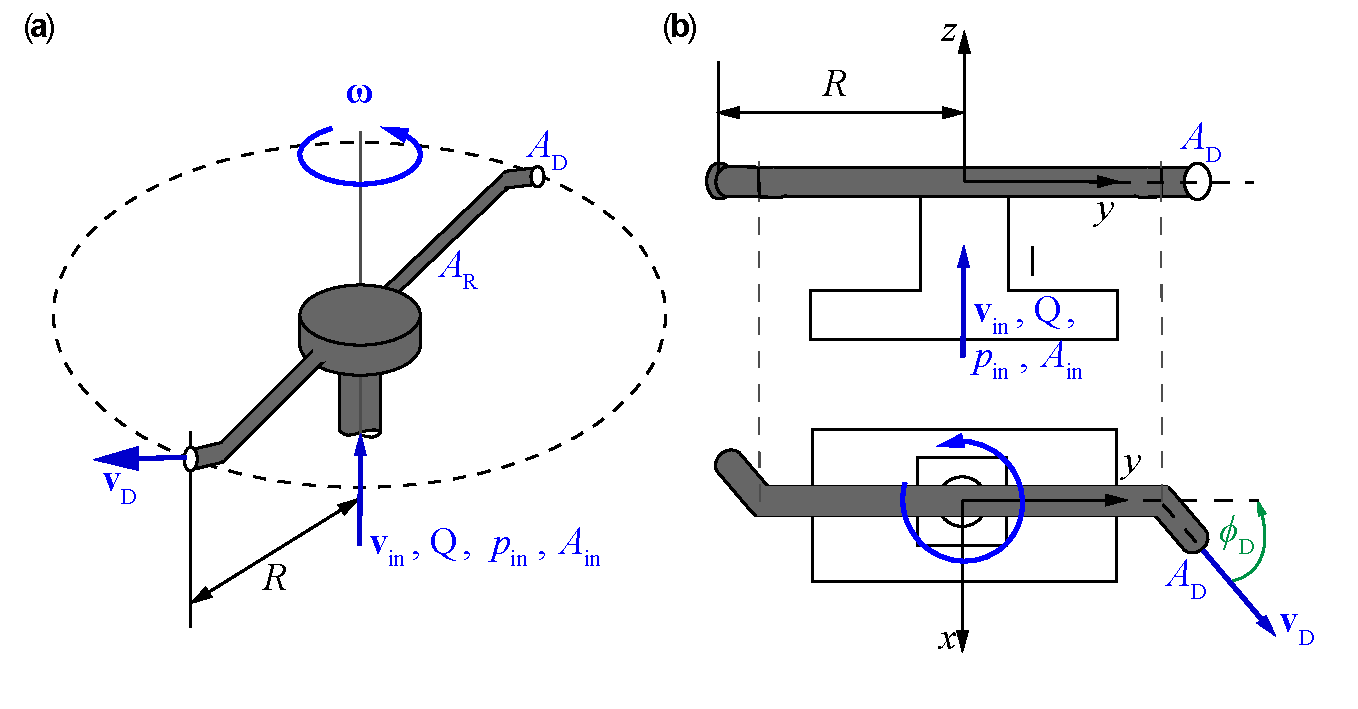
\includegraphics[width=\textwidth]{RegularSprinkler.pdf}
    \caption[Physik am Rasensprinkler.]{Physik am Rasensprinkler. \fa Prinzipaufbau und physikalische Gr��en. \fb Geometrie. Die D�sen haben einen Winkel $\phi_\text{D}$ relativ zur Tangente des durch die horizontalen Arme definierten Kreises. }
    \label{abb:kontmech_sprinkler01}
  \end{figure}
	
\begin{enumerate} 
\item [a)] \textbf{Drehzahl}\\
Mit \figref{kontmech_sprinkler01} k�nnen wir im Inertialsystem, den Drehimpuls-Drehmomenten-Satz aufschreiben.\\
\begin{align}
    \frac{\d}{\d t}\,\vec{L} = \frac{\d}{\d t}\,\lek \vec{L}_{\lk\text{Vol}\rk} + \vec{L}_{\lk\text{Aussto�}\rk}\rek = \vec{M}_{\text{Reibung}}\,. \label{kontmech_sprinkler01}
\end{align}
$\d/\d t\,\vec{L}_{\lk\text{Vol}\rk}$ ist die �nderung des Gesamtvolumens des flie�enden Wassers im Sprinkler und $\d/\d t\,\vec{L}_{\lk\text{Aussto�}\rk}$ die entsprechende Drehimpuls�nderung durch das aus der D�se ausgesto�ene Wasser. $\vec{M}_{\text{Reibung}}$ ist das Reibungsmoment.\\
Wir schreiben genauer:
\begin{align}
    \underbrace{\frac{\d}{\d t}\,\int\limits_{\lk\text{Vol}\rk}\varrho\,\vec{r}\times\vec{v}\,\D V}_{I_1} + \underbrace{\int\limits_{\lk{2 A_\text{D}}\rk}\varrho\,\vec{r}\times\vec{v}\,\lk \vec{v}_\text{D}-\vec{v}_\text{S}\rk\,\D \vec{Q}}_{I_2} =-\eta\,\vec{\omega} = -\eta\,\omega\,\veceZ\,.\label{kontmech_sprinkler02}
\end{align}
$\eta$ ist ein Koeffizient der Reibung. \\
Im station�ren Fall ist $I_1=0$. Das zweite Integral $I_2$ wird ermittelt, indem �ber die Querschnittsfl�che $A_\text{D}$ der D�sen�ffnung integriert wird. $\vec{v}_\text{D}$ ist die Geschwindigkeit des Wassers an der die D�sen�ffnung und $\vec{v}_\text{S} = \omega\,R\,\vec{e}_\phi$ die aus der Rotation resultierende Geschwindigkeit des Sprinklerarms am Ort der D�se, $Q$ ist der gesamte station�re Fluss durch die zwei Austrittsfl�chen $A_\text{D}$.\\
Die f�r den Drehimpuls relevante Austrittsgeschwindigkeit in Richtung $\vec{e}_\phi$ im Inertialsystem ist dann:
\begin{align}
    \vec{v}_\text{D}-\vec{v}_\text{S} = \frac{Q}{2}\,\frac{1}{A_\text{D}}\,\cos\phi_\text{D}\,\vec{e}_\phi-\omega\,R\,\vec{e}_\phi\,,\label{kontmech_sprinkler03}
\end{align}
worin $\phi_\text{D}$ der Winkel der D�senrichtung zur Tangente an den Kreis mit Radius $R$ (\figref{kontmech_sprinkler01})\,b ist. Damit erhalten wir f�r den station�ren Fall aus \eqref{kontmech_sprinkler02} einfach
\begin{align}
    I_2 = 2\varrho\,\frac{Q}{2}\,\lek \lk R\,\vec{e}_\text{r} \times \frac{Q}{2A_\text{D}}\,\cos\phi_\text{D}-\omega\,R\rk\,\vec{e}_\phi \rek = \eta\,\omega\,\veceZ\,. \label{kontmech_sprinkler04}
\end{align}
Hieraus erhalten wir schlie�lich
\begin{align}
    \omega= \frac{Q\,\cos\phi_\text{D}}{2A_\text{D}\,\lek R+\eta/\lk\varrho\,Q\,R\rk\rek}\,. \label{kontmech_sprinkler05}
\end{align}

Wir machen noch zum Vergleich die analogen Betrachtungen im mitbewegten Koordinatensystem, wobei wir wieder vom station�ren Fall ausgehen. Aus Gleichung \eqref{kontmech_sprinkler02} wird:
\begin{align}
    I_2 = \int\limits_{\lk{2A_\text{D}}\rk}\varrho\,\vec{r}\times\vec{v}_\text{D}\,\D Q = \vec{M}_\text{Reibung}+ \vec{M}_\text{Tr�gheit}\,.\label{kontmech_sprinkler06}
\end{align}
Hier haben wir auf der rechten Seite ein zus�tzliches Drehmoment ber�cksichtigt, was aus den Tr�gheitskr�ften (speziell der Coriolis-Kraft) im mitbewegten System resultiert. Wir werten \eqref{kontmech_sprinkler06} aus und erhalten:
\begin{align}
\begin{split}
    2\varrho\,\frac{Q}{2}\,\lek R\,\vec{e}_r \times \frac{Q}{2A_\text{D}}\,\cos\phi_\text{D}\,\vec{e}_\phi \rek &= -\eta\,\omega\,\veceZ + \int\limits_{\lk{\text{Vol}}\rk} \varrho\,\vec{r}\times\vec{f}_\text{Cor}\,\,\D V \\
    &= \eta\,\omega\,\vec{e}_z + \int\limits_{\lk{\text{Vol}}\rk} \varrho\,r\,2\omega\,v_\text{r} \,\,\D V\,\vec{e}_z
\end{split}\label{kontmech_sprinkler07}
\end{align}
mit $v_r = \vec{v}\,\vec{e}_r = Q/2A_r$ als die Str�mungsgeschwindigkeit des Wassers in den Sprinklerarmen (deren Querschnittsfl�che ist $A_r$) und der Corioliskraftdichte
\begin{align}
    \vec{f}_\text{Cor} = -2\omega\,v_r\,\vec{e}_{\phi} \,.\label{kontmech_sprinkler08}
\end{align}
Es wird \eqref{kontmech_sprinkler07} �ber das Volumenelement $\D V =A_r \,\D r$ integriert, woraus folgt:
\begin{align}
    -\varrho\,\frac{Q^2}{2A_\text{D}}\,R\,\cos\phi_\text{D} = -\eta\,\omega - 2\,\varrho\,\omega\,Q\,\int\limits_0^\text{R} r\,\D r\,. \label{kontmech_sprinkler09}
\end{align}
Hier haben wir bei der Integration �ber die Corioliskraftdichte einen Faktor 2 ber�cksichtigt, da die Corisoliskraft in den beiden Armen des Sprinklers in gleicher Weise wirkt und wir nur �ber eine Arml�nge von $0$ bis $R$ integrieren. 
Nach Umformung erhalten wir wieder:
\begin{align}
    \omega = \frac{Q\,\cos\,\phi_\text{D}}{2A_\text{D}\,\lek R+\eta / \lk \varrho\,Q\,R\rk\rek}\,, \label{kontmech_sprinkler10}
\end{align}
was nat�rlich mit \eqref{kontmech_sprinkler05} �bereinstimmt.\\
Wenn man eine station�re Umdrehungszahl von \ca $\SI{30}{\per\minute} = \SI{0.5}{\per\second}$ annimmt, erh�lt man f�r typische Werte $R=\SI{30}{\cm}$, $A_\text{D}  = \pi/4\,d_\text{D}{}^2 = \pi/4\,\SI{4}{\square\mm}$, $Q = \SI{0.1}{\cubic\dm\per\second}$, $\phi_\text{D} = 10\degree$ und $\varrho \approx \SI{1}{\kg\per\cubic\metre}$ f�r das Reibungsmoment 
\begin{equation}
	\eta = Q\,R\,\varrho\,\lek \frac{Q\,\cos\phi_\text{D}}{2A_\text{D}\,\omega}-R \rek \approx \SI{0.1}{\newton\metre\second} \,.\\ 
	\label{kontmech_sprinkler10a}
\end{equation}
Man kann sich die Fragen stellen, wie gro� $\omega$ wird, wenn die Reibung $\eta$ gegen $0$ geht? Aus \eqref{kontmech_sprinkler10} erhalten wir
    \begin{align*}
        \omega = \frac{Q\,\cos\phi_\text{D}}{2A_\text{D}\,R} ~~~~\rightarrow ~~~~ v = \omega\,R\approx\frac{Q\,\cos\phi_\text{D}}{2A_\text{D}} = v_\text{D}\,\cos\phi_\text{D}\,.
    \end{align*}
Die Tangentialgeschwindigkeit des Sprinklers am Ort der D�se wird also gleich der Ausstr�mgeschwindigkeit, was ja auch zu erwarten war.\\

\item [b)] \textbf{Wasserdruck}\\

Welchen Wasserdruck braucht man, damit bei einem Reibungskoeffizienten von $\eta=\SI{10}{\newton\metre\second}$ eine Rotationsfrequenz von $\omega = 30\ldots60\,\SI{}{\per\minute}$ zustande kommt? \\
Wir m�ssen dazu das Bernoulli-Gesetz im mitrotierenden System anwenden, da wir nur dort einen station�ren Punkt f�r die D�se und damit Anwendung des Bernoulli-Gesetzes finden k�nnen. Wir erhalten dann mit \figref{kontmech_sprinkler01}\,b:
    \begin{align}
        p_\text{L} + \underbrace{\frac{1}{2}\,\varrho\,v_\text{D}{}^2-\frac{1}{2}\,\varrho\,\omega^2\,R^2}_{\text{Ort: D�se}} = \underbrace{p_\text{in} + \frac{1}{2}\,\varrho\,v_\text{in}{}^2}_{\text{Ort: Inlet}} \,. \label{kontmech_sprinkler11}
    \end{align}
    Der dritte Term auf der linken Seite mag etwas �berraschen. Da wir aber im bewegten System sind, ist dies nichts anderes als der Druck, der durch die Zentrifugalkraft des ausstr�menden Wassers aus dem rotierenden Sprinkler hervorgerufen wird. Dieser Wert ist auch dann vorhanden, wenn der Sprinkler rotiert und der Einlass blockiert wird.
    Wir setzen $v_\text{D} = Q/A_\text{D}$, $v_\text{in} = Q/A_\text{in}$ und $p_\text{L}\approx \SI{1013e2}{\Pa}$.
    Dann folgt:
    \begin{align}
        \Delta p = p_\text{in} - p_\text{L} = \frac{1}{2}\,\varrho\,\lek \frac{Q^2}{{A_\text{D}}^2}-\frac{Q^2}{{A_\text{in}}^2}-\omega^2\,R^2\rek\,. \label{kontmech_sprinkler12}
    \end{align}
    Damit eine Rotation zustande kommt muss offensichtlich $\Delta p > 0$ und $A_\text{D}<A_\text{in}$ sein und der Flu� 
    \begin{align*}
        Q = \frac{\omega R A_\text{D}}{\sqrt{1-A_\text{D}{}^2/A_\text{in}{}^2}}\,.
    \end{align*}
		Mit unseren Werten von oben und $A_\text{in}  = \pi/4\,\SI{1.25}{\square\cm}$, erhalten wir $\Delta p/p_\text{L} \approx 1.3$, siehe dazu auch \figref{kontmech_sprinkler02}.\\
		
		
	\begin{figure}
    \centering
    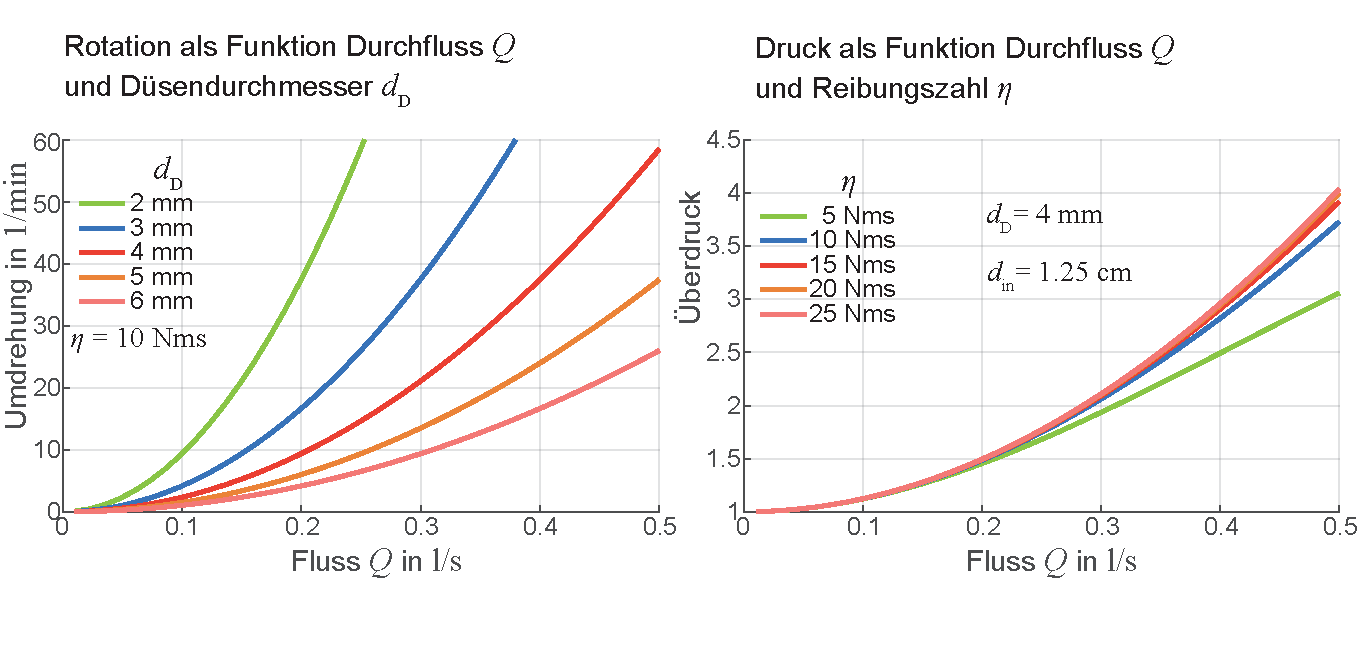
\includegraphics[width=\textwidth]{RegularSprinkler02.pdf}
    \caption[Physik am Rasensprinkler.]{Physik am Rasensprinkler. Berechnung verschiedener Parameter.}
    \label{abb:kontmech_sprinkler02}
  \end{figure}


\item [c)] \textbf{Blockierter Gartenschlauch}\\

Warum schie�t das Wasser aus einem Sprinkler \bzw einem Wasserschlauch h�her \bzw weiter, wenn man die  �ffnung teilweise blockiert? Diese scheinbar einfache Frage ist gar nicht so einfach zu beantworten. Eine alleinige Betrachtung mit der Bernoulli-Gleichung reicht nicht aus, da wir bei diesem Problem die Viskosit�t der Fl�ssigkeit mit ber�cksichtigen m�ssen. Wir empfehlen den interessierten Leser die analytischen und numerischen Betrachtungen in \cite{Alam2021} und geben hier nur eine anschauliche Erkl�rung an:\\        
Wird ein Gartenschlauch an der Ausgangs�ffnung teilweise blockiert, so kommt es zu einer Reduktion des Volumenflusses $Q$ innerhalb des Schlauches, damit auch zu einer geringeren viskosen Reibung im Schlauch und damit einen geringeren Druckabfall. Vergleiche dazu \eqref{eq:kontmech_StroemungsGeschwKreisrohr} (Gesetz von Hagen\footnote{Gotthilf Heinrich Ludwig Hagen (1797--1884) war ein deutscher Wasserbauingenieur und Hochschullehrer. Er gab das erste in deutscher Sprache erschienene Handbuch der Wasserbaukunst heraus.}\indexp{Hagen, Gotthilf Heinrich Ludwig}-Poiseuille\footnote{Jean L�onard Marie Poiseuille (1797-�1869) war ein franz�sischer Physiologe und Physiker. Er arbeitete vorwiegend auf dem Gebiet der Physiologie des Blutkreislaufs und versuchte physikalische  Erkenntnisse auf die Physiologie zu �bertragen.}\indexp{Poiseuille, Jean L�onard Marie}\index{Gesetz von Hagen-Poiseuille} genannt). Es steht also mehr Druck zur Verf�gung, der die Fl�ssigkeitsteilchen am Ende des Schlauches auf eine h�here  Geschwindigkeit beschleunigt.
\end{enumerate}

\end{sol} 
\textcolor{blue} {$\rightarrow$ zur} \probref{kontmech_rotating_sprinkler}.\\
\noindent\rule[1ex]{\textwidth}{0.5pt}  \newpage  \clearpage


%-----------------------------------------------------------------------------------------------------------


\begin{sol}{prob:kontmech_reverse_sprinkler}\label{lsg:kontmech_reverse_sprinkler} %�bung9
\textbf{Feynmans inverser Rasensprinkler}\\ \\

Eine gute Darstellung des Diskussionsstands zu allen Effekten, die uns in
dieser Aufgabe interessieren, findet sich bei Jenkins \cite{Jenkins2004}.
Tats�chlich zeigt eine neuere, sehr detaillierte Betrachtung, dass f�r ein
vollst�ndiges Bild die Geometrie in Verbindung mit Reibungseffekten sehr
genau analysiert werden muss, um mit experimentellen Beobachtungen in
Einklang zu kommen \cite{Wang2024}.

Im wesentlichen l�sst sich die Tatsache, dass der inverse Sprinkler (abgesehen
vom Anlaufen und Anhalten des Wasserflusses und ohne die asymmetrischen Effekt
aus \cite{Wang2024}) nicht zu einer Drehung angeregt wird, mit seiner
besonderen Konstruktion begr�nden. Eine vereinfachte L-f�rmige Darstellung
eines Arms des Sprinklers als wesentliches Bauteil, an dem erkl�rt werden kann,
dass das Drehmoment verschwindet, ist nach der Idee von Jenkins
\cite{Jenkins2004} in \figref{kontmech_inverserSprinklerKonstr} zu sehen.
Tats�chlich verschwindet allein schon an einem Arm das resultierende
Drehmoment. Es handelt sich nicht um einen Effekt des Ausgleichs mehrerer Arme.

\begin{figure}
  \centering
  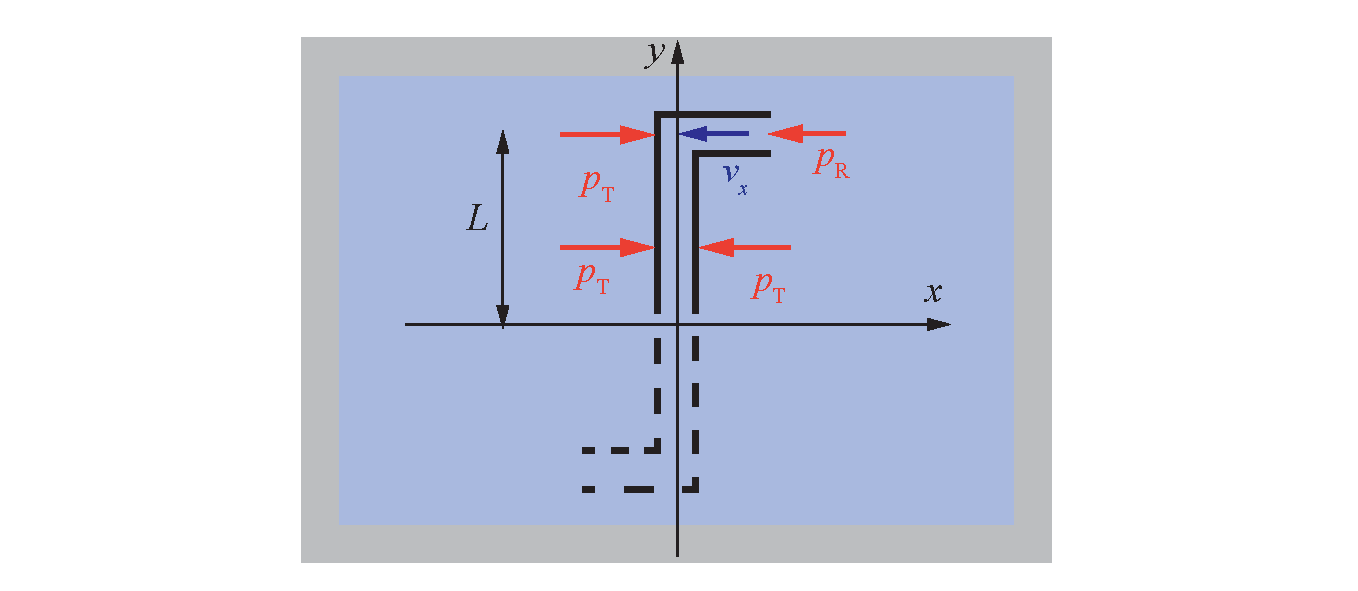
\includegraphics[width=\textwidth]{InverserSprinklerDruck.pdf}
  \caption[Aufbau des inversen Sprinklers mit Druckbilanz.]%
  {Aufbau des inversen Sprinklers mit Druckbilanz und Geschwindigkeit,
    die zu einer Impuls�nderung f�hrt.}
  \label{abb:kontmech_inverserSprinklerKonstr}
\end{figure}

Betrachten wir zun�chst die Druckbilanz, wie in der Aufgabenstellung
vorgeschlagen wird. Das Wasser des inversen Sprinklers wird in der
Beschreibung Feynmans durch eine Saugpumpe angetrieben. Somit handelt es sich
um eine Wasserbewegung, die von einem Druckuntrschied am Laufen gehalten
wird. Der Druck $p_\mathrm{R}$ im Saugrohrarm muss also geringer sein als
der Druck $P_\mathrm{T}$ im Tank, der von allen Seiten auf den Sprinklerarm
wirkt. Damit ergibt sich mit einem Rohrquerschnitt der Fl�che $A$ eine
resultirende Kraft
\begin{equation*}
  F_\mathrm{D} = (p_\mathrm{T}-p_\mathrm{R})\,A
\end{equation*}
durch den Druckunterschied auf die Wand. Mit der Arml�nge $l$ (die wir bis
zur Mitte auf der angreifenden Fl�che $A$ messen), erhalten wir daraus
ein Drehmoment von
\begin{equation*}
  M_\mathrm{D} = (p_\mathrm{T}-p_\mathrm{R})\, A\, L \; .
\end{equation*}

W�rde nur das Drehmoment durch den Druckunterschied bestehen, m�sste der
Sprinkler sich beschleunigt drehen, bis eine Reibungskraft im Gleichgewicht
zur Beschleunigung steht. Wir m�ssen jedoch auch ber�cksichtigen, dass
das Wasser an der Fl�che $A$ seine Flussrichtung �ndert. Das einstr�mende
Wasser hat einen Impuls in negative $x$-Richtung. Dieser Impuls muss
vollst�ndig abgebremst werden, was einen weitere Kraft auf den Arm
bewirkt.\footnote{Nat�rlich nimmt das Wasser auch einen Impuls in negativer
  $y$-Richtung auf, jedoch muss dieser uns nicht interessieren, da die daf�r
  notwendige Kraft vom Fu� des Sprinklers aufgebracht wird und zus�tzlich
  parallel zum Arm verl�uft und somit kein Drehmoment aus�ben kann.}
Diese Kraft k�nnen wir direkt aus der Impuls�nderung des Wassers ableiten.
Dabei ist die Kraft auf das Rohr negativ zu der, die das Rohr auf das
Wasser aus�ben muss, um dieses abzubremsen, also
\begin{equation*}
  F_\mathrm{I} = -\frac{\D m_\mathrm{W}\,v_x}{\D t} = -\frac{\D m_\mathrm{W}}{\D t}\, v_x \; .
\end{equation*}
Das Str�mungsverhalten an der Rohr�ffnung ist sicher komplex. Wir k�nnen
uns jedoch auf die Massenerhaltung verlassen. Damit die Str�mung im Rohr
station�r sein kann (und genau diesen Fall betrachten wir bisher), muss im
Zeitintervall $\D t$ gerade so viel im Tank stehendes Wasser auf die
Flie�geschwindigkeit $v_x$ im Rohr beschleunigt werden, wie im Rohr am Knick
umgelenkt wird und an $x$-Impuls verliert. Diese Beschleunigung des Wasservolumens 
geschieht aber gerade durch den Druckgradienten, sodass auch gilt
\begin{align*}
  \frac{\D m_\mathrm{W}\, v_x}{\D t} = \frac{\D m_\mathrm{W}}{\D t}\, v_x
  = F_\mathrm{D} = (p_\mathrm{T}-p_\mathrm{R})\, A \; .
\end{align*}
In Summe erh�lt man, dass $F_\mathrm{I} = - F_\mathrm{D}$, die Kraft durch den
Impuls�bertrag wirkt also genau der Kraft durch den Druckunterschied entgegen.
Gleiches gilt f�r die Drehmomente, $M_\mathrm{I} = - M_\mathrm{D}$. Der
Drehimpuls bez�glich des Fu�es des Sprinklers ist also konstant. Ist er zu
Beginn Null, bleibt er es und es kommt keine Rotation zustande.

Das war bisher nur der station�re Fall. Nun wollen wir den Anlaufprozess
betrachten. Bei diesem besteht durch die eingeschaltete Pumpe bereits
der Druckgradient. Bis das Wasser jedoch so beschleunigt wurde, dass die
Str�mung das erste Mal auf die Wand des Sprinklers am Knick trifft, fehlt
jedoch der Impuls�bertrag, der die Kraft aufgrund des Druckunterschieds
ausgleichen k�nnte. Es kommt zu einer Beschleunigung in Richtung des
offenen Endes des Rohres. Der Sprinkler bewegt sich im Uhrzeigersinn.

Genau das Gegenteil passiert beim Abschalten. Hier bricht der Druckunterschied
schlagartig ab. Das Wasser ben�tigt jedoch einige Zeit, um zum Stillstand
zu kommen. Kurzzeitig wird die Kraft aus dem Impuls�bertrag nicht ausgeglichen
und es kommt zu einer Beschleunigung vom offenen Ende weg. Insgesamt erh�lt
man damit folgendes ideales Bewegungsbild f�r einen Fall ohne Reibung: Durch
den Anlaufprozess wird eine Kreisbewegung im Uhrzeigersinn in Gang gesetzt.
Nach dem Anlaufprozess gibt es keine Beschleunigung mehr und die Kreisbewegung
setzt sich mit konstanter Winkelgeschwindigkeit fort. Mit dem Abschalten der
Pumpe kommt diese Kreisbewegung wieder zum Stehen.

Geht man genauer auf die Form und die Anordnung der D�sen ein \cite{Wang2024}, stellt sich heraus, dass
sich in der Geometrie nach \figref{kontmech_inverserSprinklerKonstr} unter Ber�cksichtigung von Reibungseffekten beim Ansaugen des
Wassers ein asymmetrischen Geschwindigkeits- \bzw Druckprofil herausbilden kann,
 \dh es gilt nicht �berall $p_\mathrm{T}=\con$. Genaueres
�berlegen f�hrt dazu, dass ein solches sogar ziemlich wahrscheinlich ist, denn das
Wasser muss ja die Biegung im Arm umstr�men. Eine solche Asymmetrie f�hrt aber
nun dazu, dass es doch ein resultierendes effektives (kleines) Drehmoment gibt, das (auch im
station�ren Fluss) eine Drehbewegung verursachen kann.\\
Dem interessierten Leser empfehlen wir die Darstellung der aktuellen "`Forschungsergebnisse"' zu dem Thema in \cite{Wang2024}.

\end{sol} 
\textcolor{blue} {$\rightarrow$ zur} \probref{kontmech_reverse_sprinkler}.\\
\noindent\rule[1ex]{\textwidth}{0.5pt}  \newpage  \clearpage

%-----------------------------------------------------------------------------------------------------------

\begin{sol}{prob:kontmech_StroemungRechteckrohr}\label{lsg:kontmech_StroemungRechteckrohr} %�bung10
\textbf{Str�mung durch Rohre}\\ \\

\begin{enumerate}

\item F�r die Str�mung durch ein Rohr, muss die Differentialgleichung
  \eqref{eq:kontmech_NaStstat}, 
  \begin{equation*}
    \eta \, \Delta \vec{v} - \nablav p = \vec{0} \; ,
  \end{equation*}
  f�r eine Fl�che senkrecht zur Str�mung gel�st werden. Wenn wir die
  Fl�che parallel zur $x$-$y$-Ebene ansehen und f�r eine station�re
  Str�mung annehmen, dass $\vec{v} = v_z(x,y) \veceZ$, also die $v_z$-Komponente
  selbst nicht von $z$ abh�ngt (vergleiche Beispiel
  \ref{bsp:kontmech_laminareStroemungen} in Kapitel
  \ref{kap:kontmech_laminareStroemungenFluessigkeiten}), so reduziert
  sich die Differentialgleichung auf
  \begin{equation*}
    \eta \, \left ( \frac{\partial^2}{\partial x^2} + \frac{\partial^2}
      {\partial y^2} \right ) v_z = \frac{\partial p}{\partial z}
  \end{equation*}
  mit einem konstanten Druckgradienten in $z$-Richtung.

  Diese partielle Differentialgleichung wird mit Hilfe der Partial
  Differential Equation Toolbox von \matlab{} gel�st und zwar mit der 
  \textcolor{mygreen}{\texttt{solvepde}}-Routine.
  Die Kreisgeometrie
  wird mit der vordefinierten Kreisfl�che des Radius 1 (entspricht in
  unserem Fall $\SI{1}{\metre}$) beschrieben. Dar�ber hinaus werden die
  Zahlenwerte $a = \SI{20}{\centi\metre}$, $b = \SI{30}{\centi\metre}$,
  $\eta = 1$ (Wasser) sowie ein angenommener geringer Druckgradient von
  $\partial p/\partial z = \SI{20}{\pascal\per\metre}$ verwendet. Das
  Beispielprogramm ist in der \matlab{}-Datei \mlkontmechref{Kreisrohr.m}
  gegeben.

  Man erh�lt die in \figref{kontmech_KreisRohrGeschwindigkeit} dargestellte
  L�sung. Der Paraboloid, den wir bereits aus Beispiel
  \ref{bsp:kontmech_laminareStroemungen} kennen, ist deutlich zu erkennen.
  Daneben ist die Differenz der numerischen und der analytischen L�sung
  aus Gleichung \eqref{eq:kontmech_StroemungsGeschwKreisrohr} gezeigt. Sie f�llt
  so klein aus, dass sie allein durch numerische Fehler zu erkl�ren ist.  
  
  \begin{figure}
    \centering
    \includegraphics[width=\textwidth]{KreisRohrGeschwindigkeit.pdf}
    \caption[Geschwindigkeitsprofil einer Str�mung in einem kreisrunden Rohr.]
    {\fa Geschwindigkeitsprofil der Str�mung durch ein kreisrundes Rohr bei einem
      konstanten Druckgradienten senkrecht zum Rohrquerschnitt. \fb Differenz zwischen der numerischen Berechnung und der
      analytischen L�sung aus \eqref{eq:kontmech_StroemungsGeschwKreisrohr}. Siehe \mscr~ \mlkontmechref{Kreisrohr.m}}
    \label{abb:kontmech_KreisRohrGeschwindigkeit}
  \end{figure}

  
\item Nun muss dieselbe Differentialgleichung auf einem rechteckigen Gebiet
  gel�st werden, das wir durch $-a/2 < x < a/2$ und $-b/2 < y < b/2$
  beschreiben. Auf dem Rand m�ssen die Dirichlet-Randbedingungen
  $v_z(-a/2,y) = v_z(a/2,y) = v_z(x,-b/2) = v_z(x,b/2) = 0$ erf�llt sein.

  Mit diesen Angaben und denselben Zahlenwerten wie im vorherigen
  Aufgabenteil erh�lt man das Beispiel, das im \matlab{}-Programm
  \mlkontmechref{Rechteckrohr.m} gegeben ist. Das Ergebnis ist in
  \figref{kontmech_RechteckRohrGeschwindigkeit} dargestellt.

  \begin{figure}
    \centering
    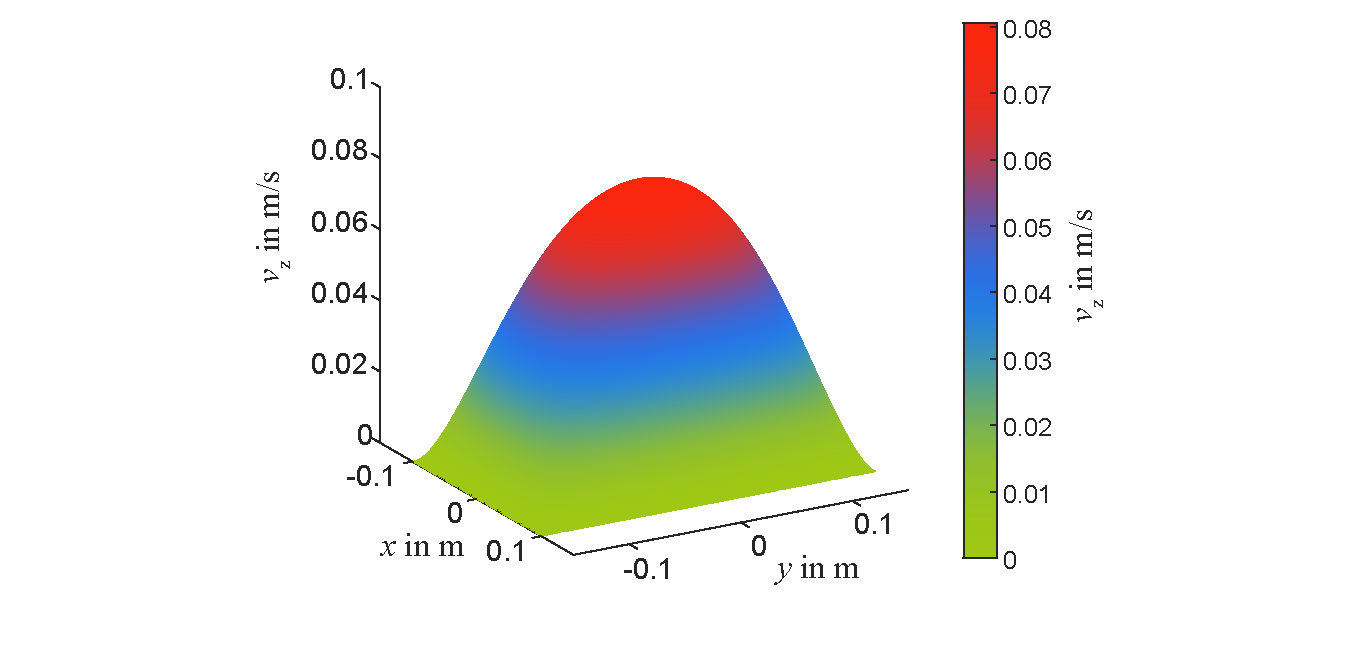
\includegraphics[width=0.8\textwidth]{RechteckRohrGeschwindigkeit.pdf}
    \caption[Geschwindigkeitsprofil einer Str�mung in einem rechteckigen Rohr.]
    {Geschwindigkeitsprofil der Str�mung durch ein rechteckiges Rohr bei einem
      konstanten Druckgradienten senkrecht zum Rohrquerschnitt.}
    \label{abb:kontmech_RechteckRohrGeschwindigkeit}
  \end{figure}
  �hnlich der L�sung im kreisrunden Rohr liegt in der Mitte
  des Rohres die h�chste Geschwindigkeit vor. Zu den R�ndern hin f�llt
  sie rasch ab. Anders als im runden Rohr ist der Abfall jedoch nicht rein
  quadratisch. Insbesondere findet man, dass er auf den Diagonalen, entlang
  derer der Weg von der Mitte zur Wand am gr��ten ist, langsamer ist als in
  der Mitte der Kanten. In den Ecken flacht das Profil erkennbar ab.
\end{enumerate}


\end{sol} 
\textcolor{blue} {$\rightarrow$ zur} \probref{kontmech_StroemungRechteckrohr}.\\
\noindent\rule[1ex]{\textwidth}{0.5pt}  \newpage  \clearpage

%-----------------------------------------------------------------------------------------------------------

\begin{sol}{prob:kontmech_StroemungTorricelli}\label{lsg:kontmech_StroemungTorricelli} %�bung11
\textbf{Str�mung aus einer Tonne - Gesetz von Torricelli}\index{Torricelli-Gesetz}\\ \\

Zur Herleitung geht man von der Bernoulli-Gleichung \index{Bernoulli-Gleichung} aus:
Man macht die Annahme, dass der Beh�lter gro� ist, so dass sich der Wasserspiegel kaum �ndert. 
Die Gr��en mit dem Index 1 gelten an der Wasseroberfl�che, die Gr��en mit dem Index 2 am Ausfluss. An der Oberfl�che ist die Geschwindigkeit $v_1$ (fast) null. Legt man die $x$-Achse in den Ausfluss, ist $h_2=0$ und $h_1$ entspricht dem H�henunterschied $H$. Der Umgebungsdruck $p_0$ sei oben und unten ann�hernd gleich gro�. Somit vereinfacht sich die Bernoulli-Gleichung zu:
\begin{align*}
\frac{v_1{}^2}{2} +\frac{p_1}{\varrho} + g\,h_1 &= \frac{v_2{}^2}{2} +\frac{p_2}{\varrho} + g\,h_2\\
\rightarrow~~~\frac{p_0}{\varrho} + g\,H &= \frac{v_2{}^2}{2} +\frac{p_0}{\varrho} \\
\rightarrow~~~\frac{p_0}{\varrho} + g\,H &= \frac{v_2{}^2}{2} +\frac{p_0}{\varrho} ~~\rightarrow v_\text{A} = v_2 =\sqrt{2g\,H}\,.\\
\end{align*}
In der Formel f�r die Austrittsgeschwindigkeit taucht der Querschnitt der Austritts�ffnung nicht auf. Damit ist auch der Auftreffpunkt des Wasserstrahls nicht von diesem Querschnitt abh�ngig. In der Praxis treten nat�rlich durch die Form der Austritts�ffnung (z.B. verrundet oder scharfkantig) und durch die Einschn�rung des Wasserstrahls teilweise starke Abweichungen der Austrittsgeschwindigkeit vom theoretischen Wert auf. Trotzdem zeigen auch viele eine verbl�ffende �bereinstimmung.

Diese Formel wurde von dem italienischen Mathematiker und Physiker Evangelista Torricelli\indexp{Torricelli, Evangelista} gefunden und nach ihm benannt.\index{Torricelli-Gleichung}

Um das Str�mungsfeld  zu berechnen, schreiben wir die Navier-Stokes-Gleichung
\eqref{eq:kontmech_NavierStokes} f�r den Fall auf, dass das Geschwindigkeitsfeld
station�r ist:
\begin{equation}
  \varrho \lk \vec{v} \cdot \nablav \rk \vec{v} = \vec{f}_\text{V}
  + \eta \, \Delta \vec{v} - \nablav p \;.
  \label{eq:kontmech_torricelli_NavierStokes}
\end{equation}
Weiterhin ber�cksichtigen wir die Konituit�tsgleichung
\eqref{eq:kontmech_KontinuitaetsglDiff}, wobei im Tank keinerlei Quellen
oder Senken existieren sollen und die Fl�ssigkeit inkompressibel sei ($\varrho =
\text{const}$):
\begin{equation}
  \frac{\partial}{\partial t}\varrho + \divv \lk \varrho\, \vec{v} \rk
  \varrho \divv \vec{v} = 0 \qquad \Rightarrow\text{d.h.} \qquad \divv \vec{v} = 0
  \; .
  \label{eq:kontmech_torricelli_kont}
\end{equation}


Die numerische L�sung des hier vorlegenden rein zweidimensionalen Problems
l�sst sich einfacher finden, wenn man das Geschwindigkeitsfeld $\vec{v}$
durch die Stromfunktion $\vec{u}$ und den Wirbelvektor $\Omega$ nach \eqref{eq:kontmech_Wirbelvektor}
ausdr�ckt. F�r die Stomfunktion gilt: 
\begin{equation}
  \vec{v} = \rotv \vec{u}
  \label{eq:kontmech_Stromfunktion}
\end{equation}
Das Einf�hren der Stromfunktion \eqref{eq:kontmech_Stromfunktion}
ist insbesondere m�glich, da sich $\vec{v}$ aufgrund der Kontinuit�tsgleichung
\eqref{eq:kontmech_torricelli_kont} als Rotation eines Vektorfeldes darstellen
lassen muss. Durch diese Darstellung ist die Kontinuit�tsgleichung automatisch
erf�llt und muss nun nicht weiter betrachtet werden.

Wir legen das Koordinatensystem so, dass die $x$-Achse in die horizontale
Richtung zeigt und die vertikale Richtung durch die $y$-Achse beschrieben
wird. Der Ursprung liegt in der linken unteren Ecke des Tanks. In diesem
Fall k�nnen wir im vorliegenden zweidimensionalen Problem
\begin{equation}
  \vec{u} = u(x,y)\veceZ
  \label{eq:komtech_torricelli_ansatzu}
\end{equation}
ansetzen und erhalten
\begin{align*}
  v_x &= \frac{\partial u}{\partial y} \;,~~~~
  v_y = -\frac{\partial u}{\partial x} \; .
\end{align*}
Weiterhin erhalten wir
\begin{equation*}
  \vec{\Omega} = \frac{1}{2} \rotv \vec{v} = \frac{1}{2} \rotv \rotv \vec{u}
  = \frac{1}{2} \lk \gradv \divv \vec{u} - \Delta \vec{u} \rk \; ,
\end{equation*}
was sich mit \eqref{eq:komtech_torricelli_ansatzu} auf
\begin{equation*}
  \vec{\Omega} = - \frac{1}{2} \Delta u(x,y)\veceZ
\end{equation*}
reduziert. Das hei�t, wir haben
\begin{equation}
  \vec{\Omega} = \Omega(x,y) \veceZ ~~~\text{und}~~~
  \Omega(x,y)  = -\frac{1}{2} \Delta u = -\frac{1}{2} \lk \frac{\partial^2}
  {\partial x^2} + \frac{\partial^2}{\partial y^2} \rk u \; .
  \label{eq:kontmech_torricelli_pdgl1}
\end{equation}

Um auch die Navier-Stokes-Gleichung durch $u$ und $\Omega$ auszudr�cken,
nehmen wir die Rotation von \eqref{eq:kontmech_torricelli_NavierStokes}.
Aus der vorherigen Berechung der Austrittsgeschwindigkeit wissen wir bereits,
dass die Volumenkraft (Gravitation) eine reine Gradientenkraft ist. Auch
der Druck hat nur einen Gradienten und keine Rotationskomponente. Entsprechend
fallen diese Terme weg. Das st�rt uns aber nicht. Die Randbedingungen,
wie sie sich durch den Fluss der Fl�ssigkeit im Gravitationsfeld ergeben,
sind durch die Berechnung der Geschwindigkeit der ausstr�menden Fl�ssigkeit
hinreichend gegeben. Wir haben nur noch das Ziel, das Geschwindigkeitsfeld
innerhalb des Tanks zu bestimmen. In den gew�hlten zweidimensionalen
Koordinaten reduziert sich die Navier-Stokes-Gleichung auf
\begin{equation}
  \varrho \lk \frac{\partial u}{\partial y}\frac{\partial \Omega}{\partial x}
  - \frac{\partial u}{\partial x}\frac{\partial \Omega}{\partial y} \rk
  = \eta \lk \frac{\partial^2 \Omega}{\partial x^2} + \frac{\partial^2 \Omega}
  {\partial y^2} \rk \; .
  \label{eq:kontmech_torricelli_pdgl2}
\end{equation}

Die Gleichungen \eqref{eq:kontmech_torricelli_pdgl1} und
\eqref{eq:kontmech_torricelli_pdgl2} bilden zusammen ein gekoppeltes,
partielles lineares Differentialgleichungssystem, das gel�st werden muss. Wichtig sind
dabei zus�tzlich die Randbedingungen, die erf�llt werden m�ssen, um das
korrekte Str�mungsbild zu erhalten.

Die numerische L�sung eines solchen Systems kann nicht einfach durch die in
\probref{kontmech_StroemungRechteckrohr} verwendete \matlab~Routine 
\textcolor{mygreen}{\texttt{solvepde}} erfolgen.
Man wendet f�r solche partiellen nichtlinearen Differentialgleichungssysteme
das sogenannte  SOR-Verfahren (�berrelaxationsverfahren)\index{SOR-Verfahren}\index{�berrelaxationsverfahren} an \cite{Meister2014}.  
Um zu sehen, wie dieses funktioniert, wollen wir dieses ausf�hrlich
anhand von Gleichung \eqref{eq:kontmech_torricelli_pdgl1} diskutieren.
Diese diskretisieren wir zun�chst,
\begin{equation*}
  \Omega(x_i,y_j) = -\frac{1}{2\Delta h^2} \left \{ u(x_{i+1},y_j)
    + u(x_{i-1},y_j) - 2 u(x_i,y_j) + u(x_i,y_{j+1}) + u(x_i,y_{j-1})
    - 2 u(x_i,y_j) \right \} \; ,
\end{equation*}
wobei wir davon ausgegangen sind, dass die Schrittweite in $x$- und
$y$-Richtung identisch ist und $\Delta h$ betr�gt.
Das l�sst sich umformen zu
\begin{align*}
  u(x_{i+1},y_j) + u(x_{i-1},y_j) + u(x_i,y_{j+1}) + u(x_i,y_{j-1})
  - 4 u(x_i,y_j) + 2\Delta h^2 \, \Omega(x_i,y_j)
  &= 0 \\
  \text{bzw.}~~~
  \frac{1}{4} \left \{ u(x_{i+1},y_j) + u(x_{i-1},y_j) + u(x_i,y_{j+1})
  + u(x_i,y_{j-1}) + 2\Delta h^2 \, \Omega(x_i,y_j) \right \} - u(x_i,y_j)
  &= 0 \; .
\end{align*}
F�r eine L�sung des Differentialgleichungssystems wird diese Gleichung
exakt erf�llt sein. Im SOR-Verfahren startet man mit Werten f�r die
$u(x_i,y_j)$ und $\Omega(x_i,y_j)$, die die Differentialgleichung
nicht l�sen werden. Es ergibt sich also eine nichtverschwindende Differenz
\begin{equation*}
  r^{(u)}_{ij} = \frac{1}{4} \left \{ u(x_{i+1},y_j) + u(x_{i-1},y_j)
    + u(x_i,y_{j+1}) + u(x_i,y_{j-1}) + 2\Delta h^2 \, \Omega(x_i,y_j)
  \right \} - u(x_i,y_j)
  \; ,
\end{equation*}
die gewichtet durch einen Konvergenzparameter (�berrelaxationsparameter)
\index{Konvergenzparameter}\index{�berrelaxationsparameter} $0\le s \le 2$
in einer Iteration auf den Wert von $u(x_i,y_j)$ aufaddiert wird,
\begin{equation*}
  u(x_i,y_j)^{(n+1)} = u(x_i,y_j)^{(n)} + s \, r^{(u,n)}_{ij}  \; ,
\end{equation*}
bis eine zufriedenstellende Konvergenz erreicht ist.

Analog l�sst sich f�r die zweite Differentialgleichung
\eqref{eq:kontmech_torricelli_pdgl2} ein Differenzparameter
\begin{multline*}
  r^{(\Omega)}_{ij} = \frac{1}{4} \bigg \{ \Omega(x_{i+1},y_j)
  + \Omega(x_{i-1},y_j) + \Omega(x_i,y_{j+1}) + \Omega(x_i,y_{j-1})  \\
    -\frac{\varrho}{4\,\eta} \bigg [ 
      \lk u(x_i,y_{j+1}) - u(x_i,y_{j-1}) \rk \lk \Omega(x_{i+1},y_j)
      - \Omega(x_{i-1},y_j) \rk \\
      - \lk u(x_{i+1},y_j) - u(x_{i-1},y_j) \rk \lk \Omega(x_i,y_{j+1})
      - \Omega(x_i,y_{j-1}) \rk \bigg ] \bigg \} - \Omega(x_i,y_j)
  \; ,
\end{multline*}
f�r die Iteration
\begin{equation*}
  \Omega(x_i,y_j)^{(n+1)} = \Omega(x_i,y_j)^{(n)} + s \, r^{(\Omega,n)}_{ij}  
\end{equation*}
finden.

In der Numerik verwenden wir die kinematische Viskosit�t $\nu
= \eta/\varrho$. Weiterhin bietet es sich an, die Symmetrie des Systems
auszunutzen und nur eine H�lfte des Tanks von der linken Wand bis zur Mitte
des Lochs zu berechnen. Dann ergeben sich die Randbedingungen dadurch, dass
kein Fluss durch die W�nde erfolgt und in der Mitte (also am rechten Rand des
berechneten Bereichs) ein Fluss senkrecht nach unten stattfindet. Ein Beispiel
f�r die Umsetzung, die auf \cite{Landau2018} beruht, kann in der 
\matlab{}-Datei \mlkontmechref{Torricelli.m} gefunden werden.

\begin{figure}
  \centering
  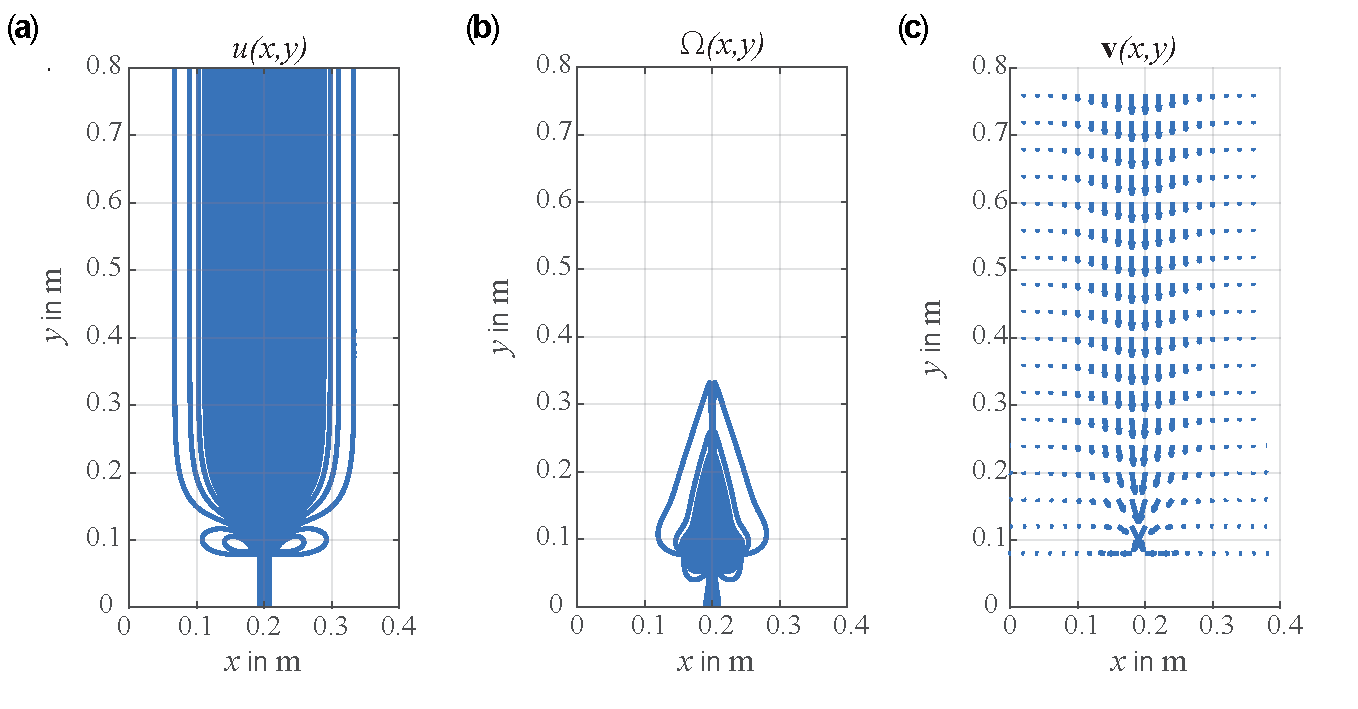
\includegraphics[width=\textwidth]{Torricelli_Fluss.pdf}
  \caption[Geschwindigkeitsprofil einer Str�mung aus einem Tank.]
  {Geschwindigkeitsprofil der Str�mung aus einem Tank bei erf�lltem Gesetz
    von Torricelli. Dargestellt sind \fa die Flusslinien (Linien mit konstantem
    $u$), \fb die Wirbellinien (Linien mit konstantem $\Omega$) sowie \fc das
    Geschwindigkeitsfeld $\vec{v}$ als Vektordiagramm.}
  \label{abb:kontmech_Torricelli_Fluss}
\end{figure}

Die Linien f�r konstantes $u$ und konstantes $\Omega$ sind in
\figref{kontmech_Torricelli_Fluss} dargestellt. Die $u$-Linien zeigen den
Fluss des Wassers an. Man erkennt das Str�men nach unten, aber auch das
Ausbilden von Wirbeln links und rechts des Ausflusses nahe am Boden. Diese
kommen dadurch zustande, dass aufgrund der Viskosit�t die zum Ausfluss
benachbarten Fl�ssigkeitsschichten mitgenommen werden. Das Nachstr�men des
Wassers f�hrt zu einer Kreisbewegung. Dem interessierten Leser wird geraten,
die kinematische Viskosit�t zu variieren, um zu beobachten, wie das zu
st�rkeren und schw�cheren Auspr�gungen der Wirbel f�hrt.

Die $\Omega$-Linien, oder Wirbellinien, zeigen an, wo der Wirbelvektor
konstant ist. Wo die Linien dicht liegen, �ndert sich der Wirbelvektor stark.
Dies ist nahe des Ausflusses der Fall und best�tigt die Beobachtung aus den
Flusslinien.

In der untersten Zeile der Abbildung sehen wir  das Geschwindigkeitsfeld als
Vektordiagramm. Es veranschaulicht noch einmal, was die Fluss- und Wirbellinien
bereits verraten. Die Fl�ssigkeit str�mt von oben zum Ausfluss, w�hrend links
und rechts von diesem am Boden Str�me zum Rand entstehen, die eine Konsequenz
der Wirbelbildung sind.

Es ist interessant, wie die Geometrie in diesem station�ren Problem zur
Ausbildung von Wirbeln f�hrt. Dem Leser wird empfohlen, den Ausfluss an die
Seite des Beh�lters zu legen, um die Ver�nderung der  Wirbelbildung zu
verfolgen. Man �berlege sich die entsprechenden Randbedingungen.


\end{sol} 
\textcolor{blue} {$\rightarrow$ zur} \probref{kontmech_StroemungTorricelli}.\\
\noindent\rule[1ex]{\textwidth}{0.5pt}  \newpage  \clearpage

%-----------------------------------------------------------------------------------------------------------

\begin{sol}{prob:kontmech_StroemungTank}\label{lsg:kontmech_StroemungTank} %�bung12
\textbf{Str�mung durch einen Tank}\\ \\

In dieser �bung k�nnen wir vollst�ndig auf die Numerik aus
\probref{kontmech_StroemungTorricelli} zur�ckgreifen. Es m�ssen erneut
die Navier-Stokes-Gleichungen f�r einen zweidimensionalen Fall gel�st werden.
Anders sind nun die Randbedingungen. Die m�ssen ber�cksichtigen:
\begin{itemize}
\item Das Einfluss- und Ausflussloch sind gleich gro�, also m�ssen direkt
  an diesen die Geschwindigkeiten den gleichen Betrag haben.
\item An den linken und rechten R�ndern gibt es oberhalb und unterhalb der
  L�cher keine Geschwindigkeit. Der Geschwindigkeitsvektor verschwidet hier.
\item Die Str�mung soll zun�chst oben entlanglaufen, da das Einflussloch
  in der oberen H�lfte des Tanks liegt. Wir nehmen also am oberen Rand eine
  kleine Geschwindigkeit nach rechts an. Am unteren Rand liegt keine
  Geschwindigkeit vor. 
\end{itemize}

L�st man das Problem numerisch mit diesen Randbedingungen, erh�lt man das
in \figref{kontmech_Tank_Fluss} dargestellte Ergebnis. Der zugeh�rige
\mscr~ \mlkontmechref{Tank.m} folgt erneut dem Vorgehen aus
\probref{kontmech_StroemungTorricelli} \bzw der Darstellung in \cite{Landau2018}.

\begin{figure}
  \centering
  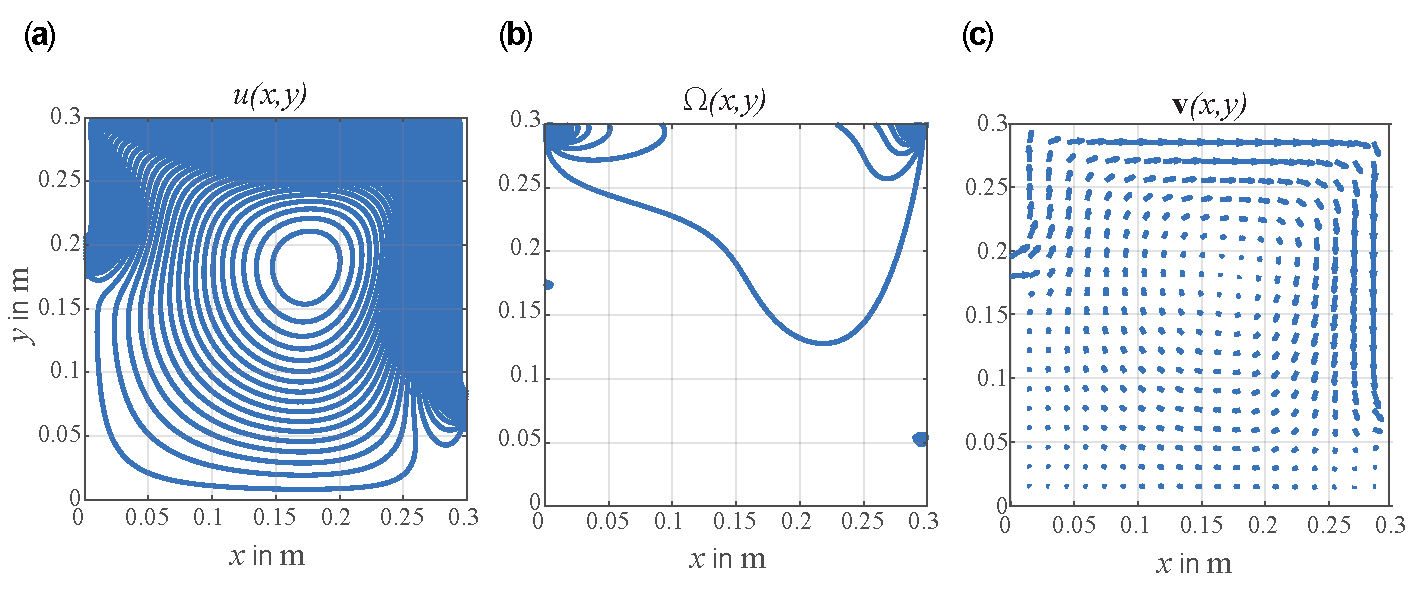
\includegraphics[width=\textwidth]{Tank_Fluss.pdf}
  \caption[Geschwindigkeitsprofil einer Str�mung durch einen Tank.]
  {Geschwindigkeitsprofil der Str�mung durch einen Tank von einem Einflussloch
    links zu einem Ausflussloch rechts. Dargestellt sind \fa die Flusslinien
    (Linien mit konstantem $u$), \fb die Wirbellinien (Linien mit konstantem
    $\Omega$) sowie \fc das Geschwindigkeitsfeld $\vec{v}$ als Vektordiagramm.}
  \label{abb:kontmech_Tank_Fluss}
\end{figure}

Tats�chlich bildet sich ein Strom der Fl�ssigkeit von links nach rechts aus,
die am oberen Rand orientiert ist.
Durch die Viskosit�t bildet sich ein Wirbel aus. Die Fl�ssigkeitsschichten,
die an die Str�mung von links nach rechts angrenzen, werden mitgenommen. Die
Kontinuit�tsgleichung (bzw. die Massenerhaltung) zwingt das Wasser zum
Nachstr�men, sodass sich ein Fluss im Kreis ausbildet.

Die Wirbellinien zeigen, dass der Wirbelvektor sich am st�rksten in den
Ecken �ndert. Dies ist zu erwarten. Bei nahezu parallelen Str�mungen muss
sich mit dem Abstand zur Wand ein Gradient der Geschwindigkeit ausbilden.

Auch hier empfehlen wir dem Leser, die gegenseitige Lage von Eintritts und Austritts�ffnung zu variieren.

\end{sol} 
\textcolor{blue} {$\rightarrow$ zur} \probref{kontmech_StroemungTank}.\\
\noindent\rule[1ex]{\textwidth}{0.5pt}  \newpage  \clearpage
%-----------------------------------------------------------------------------------------------------------

\begin{sol}{prob:kontmech_IdealerWirbel}\label{lsg:kontmech_IdealerWirbel} %�bung13
\textbf{Idealer Wirbel}\\ \\

Der Wirbelvektor \eqref{eq:kontmech_Wirbelvektor}, 
\begin{equation*}
  \vec{\Omega} = \frac{1}{2} \rotv \vec{v} \; ,
\end{equation*}
l�sst sich aus dem Geschwindigkeitsprofil berechnen. Im ersten Fall, dem
Wirbelkern, haben wir eine kreisrunde Rotation mit konstanter
Winkelgeschwindigkeit. Diese ist durch
\begin{equation*}
  \vec{v}_\mathrm{K} = r \omega \, \vec{e}_\varphi
\end{equation*}
gegeben. Damit erh�lt man den Wirbelvektor
\begin{equation*}
  \vec{\Omega}_\mathrm{K} = \frac{1}{2} \rotv \, r \omega\, \vec{e}_\varphi
  = \frac{1}{2} \, \veceZ \frac{1}{r} \frac{\partial}{\partial r} \left ( r^2
    \omega \right ) = \omega \veceZ \; .
\end{equation*}

Im �u�eren Bereich ist die Umlaufgeschwindigkeit konstant, was sich durch
\begin{equation*}
  \vec{v}_\mathrm{A} = v_\varphi \vec{e}_\varphi
\end{equation*}
mit konstantem $v_\varphi$ ausdr�cken l�sst. Der zugeh�rige Wirbelvektor lautet
\begin{equation*}
  \vec{\Omega}_\mathrm{A} = \frac{1}{2} \rotv \, v_\varphi \vec{e}_\varphi
  = \frac{1}{2} \, \veceZ \frac{1}{r} \frac{\partial}{\partial r} \left ( r
    v_\varphi \right ) = \frac{v_\varphi}{2 r} \, \veceZ \; .
\end{equation*}

An beiden Beispielen rechnen wir die Beziehung
\eqref{eq:kontmech_ZirkulationWirbelvektor} nach. Zun�chst tun wir dies
f�r den Wirbelkern. Die direkte Berechnung der Zirkulation aus der
Definition \eqref{eq:kontmech_Zirkulation} entlang des Kreises mir Radius
$R$ ergibt
\begin{equation*}
  Z_\mathrm{K} = \oint_{\partial A} \vec{v}_\mathrm{K} \cdot \D\vec{s}
  = \int_0^{2\pi} R \omega \, R \, \D \, \varphi = 2\pi\, R^2 \omega \; .
\end{equation*}
Nach \eqref{eq:kontmech_ZirkulationWirbelvektor} muss dies identisch sein
mit dem Fl�chenmittelwert des Betrags des Wirbelvektors mal der doppelten
Fl�che, also
\begin{equation*}
  Z_\mathrm{K} = \frac{2A}{A} \int_{A} \left | \vec{\Omega}_\mathrm{K}
  \right | \D A = 2 \int_{A} \left | \vec{\Omega}_\mathrm{K} \right | \D A
  = 2 \int_0^R r \, \D r \, \int_0^{2\pi}\, \D \varphi \, \omega
  = 2\pi\, R^2 \omega \; ,
\end{equation*}
was tats�chlich exakt �bereinstimmt.

F�r den �u�eren Bereich ergibt sich aus der direkten Berechnung
\begin{equation*}
  Z_\mathrm{A} = \oint_{\partial A} \vec{v}_\mathrm{A} \cdot \D\vec{s}
  = \int_0^{2\pi} \, v_\varphi \, R \, \D \, \varphi = 2\pi\, R v_\varphi \; .
\end{equation*}
�ber den Betrag des Wirbelvektors erh�lt man
\begin{equation*}
  Z_\mathrm{A} = 2 \int_{A} \left | \vec{\Omega}_\mathrm{A} \right | \D A
  = 2 \int_0^R r \, \D r \, \int_0^{2\pi}\, \D \varphi \, \frac{v_\varphi}{2 r}
  = 2\pi\, R v_\varphi \; .
\end{equation*}
Auch dies stimmt wieder �berein. Hier muss man jedoch beachten, dass die
Herleitung von \eqref{eq:kontmech_ZirkulationWirbelvektor} davon ausgeht, dass
der funktionale Zusammenhang $\vec{v} = \vec{v}(r,\varphi)$ sich nicht �ndert.
Man muss also im Fl�chenintegral immer die Form annehmen, die im �u�eren
Bereich vorliegt.


\end{sol} 
\textcolor{blue} {$\rightarrow$ zur} \probref{kontmech_IdealerWirbel}.\\
\noindent\rule[1ex]{\textwidth}{0.5pt}  \newpage  \clearpage

%-----------------------------------------------------------------------------------------------------------

\begin{sol}{prob:kontmech_UmformungWirbelsatz}\label{lsg:kontmech_UmformungWirbelsatz} %�bung14
\textbf{Helmholtzscher Wirbelsatz}\\ \\

Zum Beweis der Identit�t
\begin{equation*}
  \rotv \underbrace{\lk \lk \vec{v} \cdot \nablav \rk \vec{v} \rk}_{\vec{A}}
  = \rotv \underbrace{\lk  \rotv \vec{v} \times \vec{v} \rk}_{\vec{A}}
\end{equation*}
beginnen wir mit dem Term auf der linken Seite und subtrahieren die Rotation eines
Gradientenfeldes hinzu, was den Term nicht ver�ndert, da die Rotation
eines Gradientenfeldes immer verschwindet,
\begin{equation*}
  \rotv \lk \lk \vec{v} \cdot \nablav \rk \vec{v} \rk
  = \rotv \lk \lk \vec{v} \cdot \nablav \rk \vec{v} \rk - \rotv \frac{1}{2}
  \nablav (\vec{v}\cdot\vec{v}) \\
  = \rotv \lk \lk \vec{v} \cdot \nablav \rk \vec{v} - \frac{1}{2}
  \nablav (\vec{v}\cdot\vec{v}) \rk = \rotv \vec{A}
\end{equation*}
Den Term in der Klammer dr�cken wir nun in Indexschreibweise (siehe Kap. Mathematische Grundlagen im L�sungsteil)
aus.
\begin{align*}
  \vec{A} & = \lk \vec{v} \cdot \nablav \rk \vec{v} - \frac{1}{2}
  \nablav (\vec{v}\cdot\vec{v}) = \lk \sum_i v_i \frac{\partial}{\partial x_i} \sum_j v_j \vec{e}_j \rk
  - \frac{1}{2} \sum_j \vec{e}_j \frac{\partial}{\partial x_j} \lk
  \sum_i \vec{v}_i \vec{v}_i \rk \\
  &= \sum_i \sum_j \vec{e}_j v_i \frac{\partial v_j}{\partial x_i} 
  - \sum_i \sum_j \vec{e}_j v_i \frac{\partial v_i}{\partial x_j}\,.
\end{align*}
Im n�chsten Schritt f�hren wir zwei Kronecker-Deltas so ein, dass alle
Variablen dieselben Bezeichnungen tragen:
\begin{align*}
  \vec{A} &= \sum_i \sum_j \vec{e}_j v_i \frac{\partial v_j}{\partial x_i} 
  - \sum_i \sum_j \vec{e}_j v_i \frac{\partial v_i}{\partial x_j} \\
  &= \sum_i \sum_j \sum_l \sum_m \delta_{mj} \delta_{li} \vec{e}_j v_i
  \frac{\partial v_m}{\partial x_l} 
  - \sum_i \sum_j \sum_l \sum_m \delta_{mi} \delta_{lj} \vec{e}_j v_i
  \frac{\partial v_m}{\partial x_l} \\
  &= \sum_i \sum_j \sum_l \sum_m \lk \delta_{mj} \delta_{li}
  - \delta_{mi} \delta_{lj} \rk \vec{e}_j v_i \frac{\partial v_m}{\partial x_l} 
  = \sum_i \sum_j \sum_l \sum_m  \epsilon_{kml} \epsilon_{kji}
  \vec{e}_j v_i \frac{\partial v_m}{\partial x_l} \\
  &= - \sum_i \sum_j \sum_l \sum_m  \epsilon_{klm} \epsilon_{kji}
  \vec{e}_j v_i \frac{\partial v_m}{\partial x_l}
  = - \sum_i \sum_j  \epsilon_{kji} \vec{e}_j v_i \lk \nablav \times \vec{v}
  \rk_k \\
  &= - \sum_i \sum_j  \epsilon_{jik} \vec{e}_j v_i \lk \nablav \times \vec{v}
  \rk_k 
  = - \sum_i \sum_j  \epsilon_{jki} \vec{e}_j \lk \nablav \times \vec{v}
  \rk_k v_i = \lk \nablav \times \vec{v} \rk \times \vec{v} = \rotv \vec{v} \times \vec{v} = \vec{A}\,.
\end{align*}
Zusammenfassend erhalten wir also die gesuchte Identit�t.


\end{sol} 
\textcolor{blue} {$\rightarrow$ zur} \probref{kontmech_UmformungWirbelsatz}.\\
\noindent\rule[1ex]{\textwidth}{0.5pt}  \newpage  \clearpage

%-----------------------------------------------------------------------------------------------------------

\begin{sol}{prob:kontmech_fluesse}\label{lsg:kontmech_fluesse} %�bung15
\textbf{Ist der Rhein laminar oder turbulent?}

  \begin{figure}
    \centering
    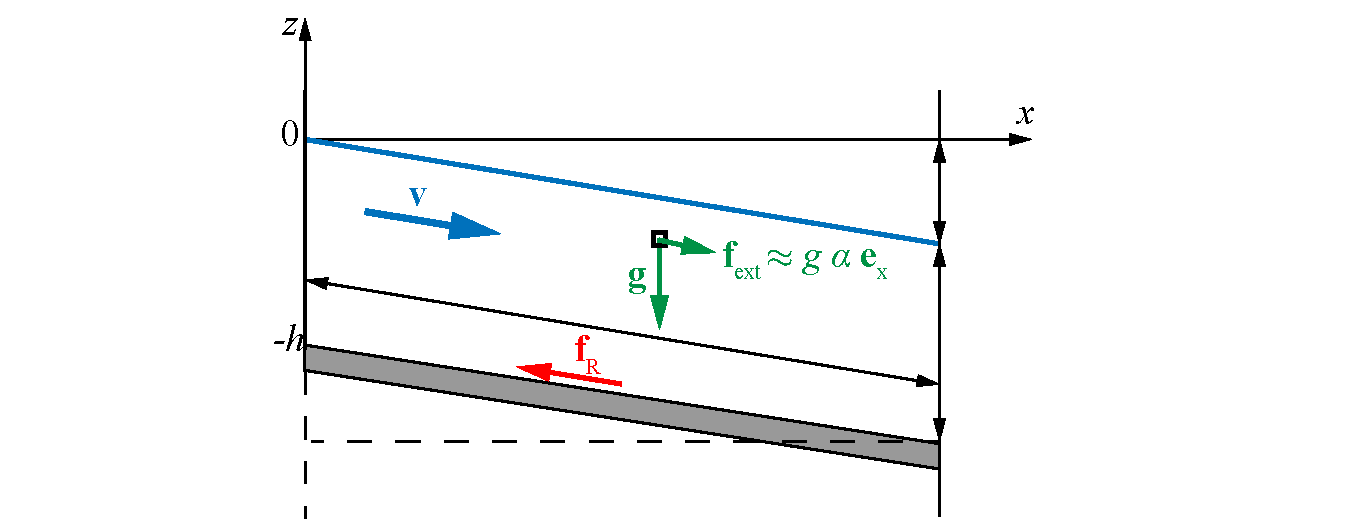
\includegraphics[width=\textwidth]{Flussgefaelle.pdf}
    \caption[Flussgef�lle mit gleichf�rmiger Wasserspiegellage.]
    {Flussgef�lle mit gleichf�rmiger Wasserspiegellage.}
    \label{abb:kontmech_fluesse01}
  \end{figure}

Wir betrachten mit \figref{kontmech_fluesse01} einen Fluss mit einer Tiefe $h$ und einem Gef�lle von 
\begin{align}
    \alpha =   \arctan \frac{\Delta h}{l} \approx \frac{\Delta h}{l} \ll 1\,. \label{eq:kontmech_fluesse01}
\end{align}
Auf ein Volumenelement des Wassers wirkt dann in $x-$-Richtung die externe (Gravitations-) Kraft:
\begin{align}
    \vec{f}_\text{ext} = -\varrho\,g\,\sin\alpha\,\veceX \approx \varrho\,g\,\alpha\,\veceX \,. \label{eq:kontmech_fluesse02}
\end{align}
F�r die inkompressible Fl�ssigkeit nehmen wir ferner an, dass die Breite des Flusses sehr viel gr��er ist als die H�he, sowie das Gef�lle konstant ist, so dass die Ableitungen der Geschwindigkeit nach $y$ und $x$ vernachl�ssigt werden k�nnen. \\
Die \NVS wird dann im laminaren Fall einfach:
\begin{align}
    0 = \vec{f}_r-\vec{f}_\text{ext} =\lk \eta\,\frac{\d^2v_x}{\d z^2}-\varrho\,g\,\alpha\rk\,\veceX\,, \label{eq:kontmech_fluesse03}
\end{align}
mit den Randbedingungen:
\begin{align*}
    z= 0:~~v_x = v_\text{F}~~~\text{\bzw}~~~z = -h:~~v_x = 0\,. 
\end{align*}
Daraus erhalten wir:
\begin{align}
    v\lk z\rk = \frac{1}{2}\,\frac{\varrho\,g\,\alpha}{\eta}\,\lk h^2-z^2\rk ~~~~~~~~0\geq z \geq -h \label{eq:kontmech_fluesse04}
\end{align}
Wir �berpr�fen f�r typische Parameter die Reynoldszahl Re ($h=\SI{2}{\metre}$, $\alpha= \SI{2e-3}{}$, $\eta = \SI{e-3}{\kg\per\metre\per\second}$), indem wir zun�chst $v_\text{F} = \frac{1}{2}\,\varrho\,g\,\alpha\,h^2/\eta$ berechnen. Mit den Parametern w�rden daraus v�llig unrealistische $v_\text{F} = \SI{20e3}{\metre\per\second}$ folgen. Umgekehrt erh�lt man bei einer typischen (schon gro�en) Flussgeschwindigkeit von $\SI{5}{\metre\per\second}$ und einem Volumenstrom (Durchflussrate) von $Q=v\,b\,h\approx \SI{100}{\cubic\metre\per\second}$ ergeben sich eine Reynoldszahl von  $\Re = \varrho\,v\,h/\eta \approx \SI{e6}{}$, 
\dh wir sind in jedem Fall im turbulenten Bereich. Der Ansatz eines laminaren Flusses und einer Reibung nach \eqref{eq:kontmech_fluesse03} ist also zu verwerfen.\\
Man kann nun f�r die Flie�geschwindigkeit $v_\text{F}$ verschiedene (halb) empirische Ans�tze machen, indem man die mittlere Flie�geschwindigkeit $\bar{v}_\text{F}$ des Gew�ssers in Beziehung zu einer Reibungskraft setzt, die sich aus der Turbulenz ergibt. Ein einfacher (Newtonscher) Ansatz f�r die Reibung besteht in:
\begin{align}
    \vec{f}_\text{R} = C\,\varrho\,\frac{\vec{v}_\text{F}{}^2}{h}\,\veceX\,,\label{eq:kontmech_fluesse05} 
\end{align}
worin $C$ ein (halb) empirischer Faktor ist, der die Reibungskraft in Bezug auf die Oberfl�cheneigenschaften des Flussbettes beschreibt. 
Man muss beachten, dass $h$ im Nenner eine Zunahme der Reibung mit geringer Wassertiefe bedeutet!\\
Mit \eqref{eq:kontmech_fluesse03} erh�lt man dann die Formel von Brahms\footnote{Albert Brahms (1692--1758) war ein bedeutender deutscher Deichbaupionier, der bereits 1757 wesentlichen noch heute g�ltige Grundlagen der Deich- und Wasserbaukunst ver�ffentlichte.} 
-Ch�zy\footnote{Antoine de Ch�zy (1718--1798) war ein franz�sischer Hydraulik-Ingenieur.}:
\begin{align*}
    \bar{v}_\text{F,BC} = C\,\sqrt{h\,\alpha\,g}\,.
\end{align*}
Ein anderer Ansatz besteht in der sogenannten Gauckler\footnote{Philippe Gaspard Gauckler (1826--1905) war ein franz�sischer Tiefbauingenieur.}-Manning\footnote{Robert Manning (1816--1897) war ein irischer Ingenieur. Er ver�ffentlichte 1891 die sp�ter unter Gauckler-Manning-Strickler-Flie�formel bekannte Formel in dem Artikel "`On the flow of water in open channels and pipes"' in Irland.}-Strickler\footnote{Albert Strickler (1887--1963) war ein Schweizer Maschinenbau- und Wasserbauingenieur, der durch seine Beitr�ge zur Fluiddynamik bekannt wurde.}\indexp{Brahm, Albert}\indexp{Ch�zy, Antoine de}\indexp{Gauckler, Philippe Gaspard}\indexp{Manning, Robert}\indexp{Strickler, Albert}-Formel. 
\begin{align*}
    \bar{v}_\text{F, GMS} = k_\text{S}\,\sqrt{\alpha}\,\sqrt[3]{h^2}\,.
\end{align*}
Aus der Literatur \cite{Martin2009} findet man f�r die Parameter $C$ \bzw $k_\text{S}$, die im Wesentlichen von der Rauigkeit des Flussbettes abh�ngen f�r Schotter-Werte im Bereich von $C = 20$ \bzw $k_\text{S} = \SI{30}{\per\cubic\metre\per\second}$ liegen. F�r den (turbulenten) Rhein ($\alpha= \SI{2e-4}{}$, $h = \SI{6}{\metre}$) ergibt sich daraus eine mittlere Flie�geschwindigkeit von
\begin{align*}
    \bar{v}_\text{F, BC} \approx \SI{1.52}{\metre\per\second} ~~~~ \text{\bzw} ~~~~ \bar{v}_\text{F, GMS} \approx \SI{1.41}{\metre\per\second}\,,
\end{align*}
was gut mit den beobachteten Geschwindigkeiten �bereinstimmt.\\
Die numerische Behandlung ist nicht trivial und stellt gegen�ber den in \probref{kontmech_StroemungRechteckrohr} \bzw \probref{kontmech_StroemungTank} dargestellten Verfahren, die sich jeweils auf laminare Probleme beziehen, eine nochmalige Komplikation dar. Das Problem ist dabei, dass auf Grund der Turbulenz die einzelnen Str�mungsgr��en (vor allem $\vec{v}\lk \vec{r},t\rk,\, p\lk \vec{r},t\rk$) in ihrem zeitlichen Verlauf und r�umlichen Strukturen nicht aufgel�st werden k�nnen (Speicherbedarf, Rechenkapazit�t).
Man arbeitet daher mit einer modifizierten Form der \NVS, den sogenannten Reynolds-Gleichungen\index{Reynolds-Gleichungen}, bei denen die einzelnen Str�mungsgr��en (\zb $\vec{v},\, p$) durch einen zeitlichen Mittelwert und eine Schwankungsgr��e ausgedr�ckt werden, also:
\begin{align*}
    \vec{v} = \bar{\vec{v}}+\vec{v}' ~~~~ \text{und} ~~~~ p = \bar{p} + p'\,.
\end{align*}
Die Reynoldsgleichungen f�r die inkompressible Fl�ssigkeit folgen dann, wenn man Dichte- und Viskosit�tsschwankungen vernachl�ssigt, \dh
\begin{align*}
    \frac{\d\rho}{\d t} &= 0 \leftrightarrow \rho = \text{const.} ~~~\text{\bzw}~~~
    \frac{\d\eta}{\d t} = 0 \leftrightarrow \eta = \text{const.}
\end{align*}
in Komponentenschreibweise aus der \NVS
\begin{align}
        \rho\,\frac{\d v_i}{\d t} + \rho\,\lk \frac{\d v_i v_j}{\d x_j}\rk &= f_\text{ext,i} - \frac{\d p}{\d x_i} + \eta\,\frac{\d}{\d x_j}\,\lk \frac{\d v_i}{\d x_j} + \frac{\d v_j}{\d x_i}\rk \label{eq:kontmech_reynoldsequ01a}
\end{align} 
zu				
\begin{align}
  \rho\,\frac{\d \bar{v}_i}{\d t} + \rho\,\lk \frac{\d \bar{v}_i \bar{v}_j}{\d x_j}\rk &= \bar{f}_\text{ext,i} - \frac{\d \bar{p}}{\d x_i} + \frac{\d}{\d x_j}\,\lk \eta \lk \frac{\d \bar{v}_i}{\d x_j} + \frac{\d \bar{v}_j}{\d x_i}\rk - \underbrace{\rho\,\overline{v_i'v_j'}}_{\substack{\text{RST}}}\rk\,,
\label{eq:kontmech_reynoldsequ01b}
\end{align} 
wobei $\overline{v_i'v_j'}$ die zeitliche Mittelung �ber die Schwankungsgr��en bedeutet. Die Reynolds-Gleichungen als modifizierte Form der Navier-Stokes-Gleichungen enthalten damit durch die Einf�hrung der Schwankungsterme den sogenannten Reynolds-Spannungstensor RST als zus�tzliche Unbekannte im Gleichungssystem. 
Wir betrachten den RST genauer:
\begin{align}
    -\mathrm{RST}_{ij}=-\sigma_{ij} = \rho\,\overline{v_i'v_j'}= \rho\,
    \begin{pmatrix}
        \:\overline{v_1'\,v_1'}\: & \overline{v_1'\,v_2'}\: & \overline{v_1'\,v_3'}\:\\
        \:\overline{v_2'\,v_1'}\: & \overline{v_2'\,v_2'}\: & \overline{v_2'\,v_3'}\:\\
        \:\overline{v_3'\,v_1'}\: & \overline{v_3'\,v_2'}\: & \overline{v_3'\,v_3'}\:
    \end{pmatrix}\label{eq:kontmech_reynoldsequ02}
\end{align}
Die Diagonalelemente des Tensors stellen Normalspannungen dar, w�hrend die Nichtdiagonal-Elemente Schubspannungen sind.\\
F�r die Berechnung dieser unbekannten Gr��en stehen allerdings nicht mehr Gleichungen zur Verf�gung. Das Gleichungssystem ist \eqref{eq:kontmech_reynoldsequ01b} ist damit nicht mehr geschlossen. Die "`Schlie�ung"' erreicht man durch zus�tzliche Annahmen f�r die Komponenten des Reynolds-Spannungstensors in Form von zus�tzlichen Gleichungen, die im Prinzip Turbulenzmodelle darstellen. Meist beruhen diese semi-empirischen Modellen und werden urch Experimente verifiziert.\\
In den meisten F�llen beruhen die Modelle auf einem Zusammenhangs zwischen den Schwankungstermen und einer gewissen makroskopischen Gr��e $\mu_i$, die als turbulente Viskosit�t bezeichnet wird.\\
Bei den sogenannten Wirbelviskosit�tsmodellen werden die Reynoldsspannungen in Analogie zur �blichen molekulare Viskosit�t $\eta$ hervorgerufenen Spannungen hervorgerufene Spannungen behandelt. Der Reynolds-Spannungstensor lautet folgt approximiert:
\begin{align}
    \rho\,\overline{v_i'v_j'} = -\mu_i\,\lk \frac{\d \bar{v}_i}{\d x_j} + \frac{\d \bar{v}_j}{\d x_i} \rk+ \frac{2}{3}\,\rho\,k\,\delta_{ij}\,.
		\label{eq:kontmech_reynoldsequ03}
\end{align}
Die turbulente Wirbelviskosit�t $\mu$ hat die Dimension $\SI{}{\metre\squared\per\second}$ und beschreibt die Erh�hung der molekularen Viskosit�t durch turbulente Schwankungsbewegungen. In der Regel �berschreitet $\mu$ die molekulare Viskosit�t deutlich. Der Term $\frac{2}{3}\,\rho\,k\,\delta_{ij}$ ist ein \anf{turbulenter Druckterm}, der notwendig ist, um Gleichungen auch f�r Normalspannungen anwenden zu k�nnen (\vgl auch \probref{kontmech_StokesReibung} und \cite{Hoffmann2000}). \\
Mit einem Turbulenzmodell nach \eqref{eq:kontmech_reynoldsequ03} kann die tats�chliche numerische L�sung wie in \probref{kontmech_StroemungRechteckrohr} durch die Finite-Differenzen Methode (FDM) erfolgen. Bei dieser Methode werden die partiellen Differentialgleichungen (Reynolds-Gleichungen) durch Differenzen approximiert und die Unbekannten an den Knotenpunkten mittels Taylor-Reihen ausgedr�ckt. Je nach Genauigkeitsanspruch k�nnen diese bei Gliedern h�herer Ordnung abgebrochen werden. Die partiellen Differentialgleichungen werden auf diese Weise in ein System algebraischer Gleichungen umgeformt \cite{Hoffmann2000, Tu2024}. \\
In der Praxis existiert eine Vielzahl an kommerziellen Softwarepaketen, in denen diese numerischen Verfahren implementiert sind. Diese Anwendung erm�glicht eine relativ \anf{bequeme} Berechnung beziehungsweise Simulation von Str�mungsvorg�ngen verschiedener Fluide. 
FLOW-3D\textregistered\, ist eines dieser Softwarepakete. Mit dessen Hilfe k�nnen viele Problemstellungen der Str�mungsmechanik gel�st werden. Ein Spezialgebiet sind Str�mungen von Fluiden mit freien Oberfl�chen. Wir empfehlen dem interessierten Leser, sich bei \url{www.flow3d.com} \bzw \cite{Tu2024, Hoffmann2000} einen �berblick zu verschaffen.

\end{sol} 
\textcolor{blue} {$\rightarrow$ zur} \probref{kontmech_fluesse}.\\
\noindent\rule[1ex]{\textwidth}{0.5pt}  \newpage  \clearpage
%-----------------------------------------------------------------------------------------------------------

\begin{sol}{prob:kontmech_StokesReibung}\label{lsg:kontmech_StokesReibung} %�bung16
\textbf{Stokes-Reibung}\index{Stokes-Reibung}\\ \\

Es gibt verschiedene Herleitungen der Stokes-Formel\footnote{Sir George Gabriel Stokes\indexp{Stokes, Sir George Gabriel} (1819--1903) war ein irischer Mathematiker und Physiker. Er arbeitete auf dem Gebiet der mathematischen und experimentellen Physik und besch�ftigte sich haupts�chlich mit der Hydrodynamik, der Elektrodynamik und der Akustik.Seine ber�hmte Formel ver�ffentlichte er erstmalig 1851 unter dem Titel "'On the effect of the internal friction of fluids on the motion of pendulums."' in den Transactions of the Cambridge Philosophical Society, Band 9, 1861, S. 8�106.}. Wir folgen hier im wesentlichen der exzellenten Darstellung in \cite{Schmutzer2005} folgen, die wir durch eine Plausibilit�tsbetrachtung, einen Einschub zum Spannungstensor und numerische Rechnungen erg�nzen.\\

\textbf{Absch�tzung, Plausibilit�tsbetrachtung}\\

Wir wollen zun�chst mit Hilfe von \figref{kontmech_stokesformel01} eine Absch�tzung treffen. Wir betrachten eine station�r flie�ende, inkompressible z�he Fl�ssigkeit ohne �u�ere Kr�fte, in der sich eine Kugel befindet. Im gro�en Abstand von der Kugel mit dem Radius $R_0$ hat die Str�mung eine konstanten Geschwindigkeit $\vec{v}_0 = v_0 \,\veceX$, auf der Kugeloberfl�che ist die Geschwindigkeit Null.  Wir k�nnen davon ausgehen, dass in einer Entfernung von $\approx\,R_0$ von der Kugeloberfl�che die Geschwindigkeit $\vec{v}_0$ nahezu wieder erreicht, was einem Geschwindigkeitsgradient von ungef�hr $\vec{v}_0/R_0$ entspricht. Nach \eqref{eq:kontmech_ReibungskraftInnere} entspricht das einer inneren Reibungskraft, die sich mit der Viskosit�t $\eta$ als Proportionalit�tsfaktor 
zu \begin{equation}
  \vec{F}_\text{R} \approx \eta \, A \, \frac{\partial v_z}{\partial y} \veceZ \approx \eta \, 4 \pi R_0{}^2 \,\frac{v_0}{R_0} \veceZ \approx  4\pi R_0{} v_0 \veceZ \;
  \label{eq:kontmech_kontmech_stokesformel_approx}
\end{equation}
ergibt. Das ist schon mal die richtige Gr��enordnung, wir werden im Folgenden sehen, dass die genaue Ber�cksichtigung der Geometrie bei der L�sung der \NVS{} einen 1.5 mal gr��eren Wert der Kraft ergibt.

  \begin{figure}
    \centering
    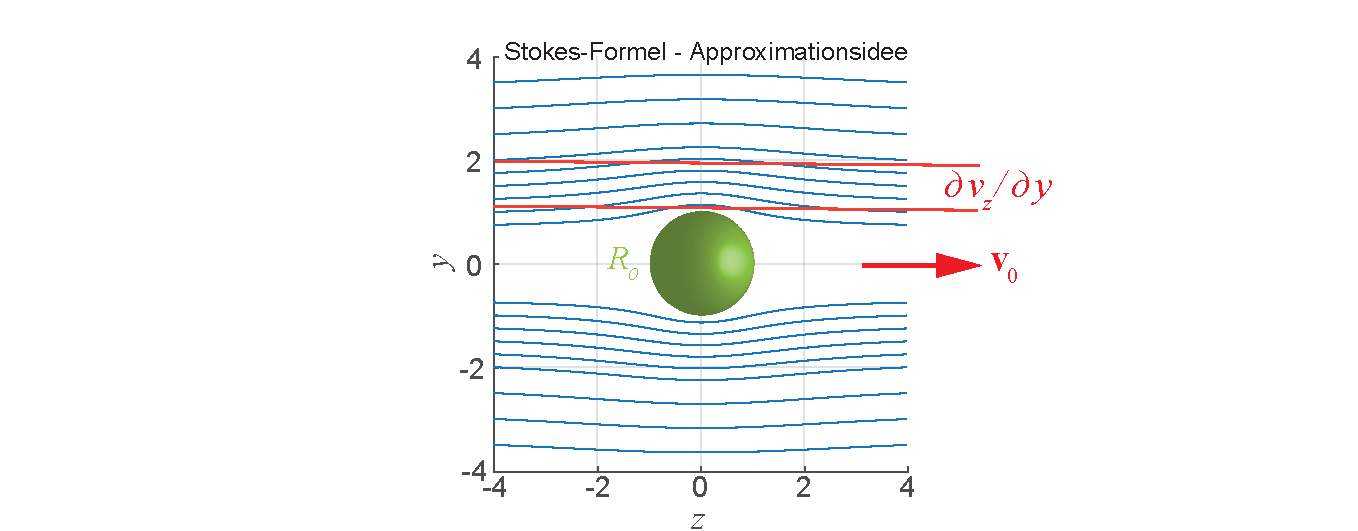
\includegraphics[width=\textwidth]{StokesFormel01.pdf}
    \caption[Geschwindigkeitsprofil einer viskosen Str�mung um eine Kugel (N�herung).]
    {Geschwindigkeitsprofil einer viskosen Str�mung um eine Kugel (N�herung).}
				\label{abb:kontmech_stokesformel01}
  \end{figure}

\textbf{Berechnung des Geschwindigkeitsfeldes aus der f�r den Stokes-Fall vereinfachten \NVS}\\

Neben der Kontinuit�ts- \bzw Inkompressibilit�tsgleichung \eqref{eq:kontmech_KontinuitaetsglInkompr} 
\begin{align}     
\divv\,\vec{v} = 0 ~~~~~~~~~ \text{mit}~~~ \varrho = \varrho_0 = \con \label{eq:kontmech_Stokes01} 
\end{align} 
ist also die Navier-Stokes-Gleichung \eqref{eq:kontmech_NavierStokesFrei}
\begin{align}   \varrho_0\,\lk\vec{v}\,\nablav\rk\,\vec{v} = -\gradv \,p + \eta\,\Delta\,\vec{v} \label{eq:kontmech_Stokes02}
\end{align} 
zu l�sen, wobei die Randbedingungen folgenderma�en lauten: 
\begin{align} ~~~~ \vec{v}(r~\rightarrow~\infty) = \vec{v}_0 = v_0\, \veceZ ~~~~~\text{und}~~~~~ \vec{v}(r~\rightarrow~R_0)= 0\,. \label{eq:kontmech_Stokes03} 
\end{align} 
Die zweite Randbedingung bringt das Haften der Fl�ssigkeit an der Kugeloberfl�che zum Ausdruck (no slip).\\

Wir linearisieren die \NVS{} unter der Annahme kleiner Reynolds-Zahlen, \dh 
$ \Re = \varrho_0 R_0 v_0\,/\,\eta_0 \,\ll\,1\,.$ Wir erhalten dann aus \eqref{eq:kontmech_Stokes02} 
\begin{align}     
\Delta\, \vec{v} = \frac{1}{\eta}\,\gradv \,p ~~~\text{und}~~~
  \rotv \lk \Delta \vec{v}\rk = 0\,. \label{eq:kontmech_Stokes05}
\end{align} 
Einen L�sungsansatz f�r die zweite Gleichung ist durch
\begin{align}     
 \vec{v} = \gradv \,\Psi + \bar{\vec{v}} ~~~~~~ \text{mit} ~~~ \Delta \bar{\vec{v}} = 0\,. \label{eq:kontmech_Stokes06} 
\end{align} 
gegeben.\footnote{Man beachte dabei die Vertauschbarkeit der partiellen Ableitungen.} Unter Ber�cksichtigung der Randbedingungen l�sen wir \eqref{eq:kontmech_Stokes06} f�r $r\neq 0$ durch 
\begin{align}     
\bar{\vec{v}} = \vec{v}_0\,\frac{A}{r} \,, \label{eq:kontmech_Stokes07} 
\end{align} 
worin $A$ eine Integrationskonstante ist.
Mit \eqref{eq:kontmech_Stokes01} folgt aus \eqref{eq:kontmech_Stokes06} 
\begin{align}     
\Delta\Psi = -\divv\,\bar{\vec{v}} = -A\,\vec{v}_0\,\gradv\lk\frac{1}{r}\rk = \frac{A}{r^2}\lk \vec{v}_0\,\vec{e}_r\rk  = \frac{A}{r^3}\lk \vec{v}_0\,\vec{r}\rk \,. \label{eq:kontmech_Stokes09} 
\end{align} 
Wir suchen nun eine L�sung dieser inhomogenen Differentialgleichung f�r $\Psi$. Wir versuchen den Ansatz \begin{align}    
\Psi = \lk \vec{v}_0\,\vec{r}\rk\,\Phi\lk r\rk\,,\label{eq:kontmech_Stokes10} 
\end{align} 
aus dem sich 
\begin{align}     
 \gradv\Psi = \lk \vec{v}_0\,\vec{r}\rk \,\gradv\Phi +\vec{v}_0\,\Phi ~~~~~~\text{und} ~~~~ \Delta\Psi = \lk \vec{v}_0\,\vec{r}\rk\,\Delta \Phi +2\vec{v}_0\,\gradv \Phi 
\label{eq:kontmech_Stokes11} 
\end{align} 
ergeben. Mit \eqref{eq:kontmech_Stokes09} erhalten wir die gew�hnliche inhomogene Differentialgleichung 
\begin{align}     
\Delta \Phi +\frac{2\vec{r}}{r^2}\,\gradv \Phi = \frac{A}{r^3} ~~~~ \text{\bzw} ~~~~~ \Phi'' +\frac{4}{r}\,\Phi' = \frac{A}{r^3}\,. \label{eq:kontmech_Stokes12} 
\end{align} 
Dabei bedeutet $\Phi'$ die Ableitung nach $r$ (Kugelkoordinate). Die homogene Differentialgleichung l�sen wir mit dem Potenzansatz 
\begin{align}     \Phi^{\lk h\rk} = r^\lambda\,, \label{eq:kontmech_Stokes13} 
\end{align} 
der auf $\lambda^2 + 3\lambda = 0$ und damit $\lambda_1 = 0\,, ~~\lambda_2 = -3$ f�hrt. F�r die L�sung der inhomogenen Gleichung ergibt sich
\begin{align}     
\Phi^{\lk \text{inh}\rk} = -\frac{A}{2r}\,, \label{eq:kontmech_Stokes14} 
\end{align} 
und damit folgt die allgemeine L�sung zu 
\begin{align}     \Phi = a + \frac{b}{r^3} - \frac{A}{2r} \,, \label{eq:kontmech_Stokes15} 
\end{align} 
worin $a,\,b\,$ Integrationskonstanten sind. 
�ber \eqref{eq:kontmech_Stokes10} und \eqref{eq:kontmech_Stokes06} ergibt sich damit f�r f�r das Geschwindigkeitsfeld:
\begin{align}     
\vec{v} = \frac{\vec{r}\,\lk \vec{v}_0\,\vec{r}\rk}{r^3}\,\lk -\frac{3b}{r^2}+\frac{A}{2}\rk + \vec{v}_0\,\lk a+\frac{b}{r^3} + \frac{A}{2r}\rk \,. \label{eq:kontmech_Stokes16} 
\end{align} 

Die Erf�llung der ersten Randbedingung liefert $a=1$ und aus der zweiten ergibt sich
\begin{align}     
\frac{\vec{r}_0\,\lk \vec{v}_0\,\vec{r}_0\rk}{R_0{}^3}\,\lk \frac{A}{2} - \frac{3b}{R_0{}^2}\rk + \vec{v}_0\,\lk 1 +\frac{b}{R_0{}^3} +\frac{A}{2R_0}\rk = 0 \,, \label{eq:kontmech_Stokes17} 
\end{align} 
wobei $\vec{r}_0$ der auf die Kugeloberfl�che zeigende winkelabh�ngige Radiusvektor ist. Aus dieser Gleichung folgt das Verschwinden der Koeffizienten 
\begin{align}     \frac{A}{2} - \frac{3b}{R_0{}^2} = 0~~~~\text{und}~~~~~ 1+\frac{b}{R_0{}^3} + \frac{A}{2R_0} = 0\,, \label{eq:kontmech_Stokes18} 
\end{align} 
da die Gleichung f�r alle $\vec{r}_0$ gelten muss. Die Aufl�sung dieser beiden Gleichungen ergibt 
\begin{align}     
A= -\frac{3R_0}{2}\,, ~~~~ b=-\frac{R_0{}^3}{4}\,, \label{eq:kontmech_Stokes19} 
\end{align} 
so dass sich das Geschwindigkeitsfeld  \eqref{eq:kontmech_Stokes16} endg�ltig als 
\begin{align}     
\vec{v} = \vec{v}_0\,\lek 1-\frac{R_0}{4r}\,\lk 3 + \frac{R_0{}^2}{r^2}\rk\rek -\vec{e}_r\,\frac{3R_0\,\lk \vec{v}_0\,\vec{e}_r\rk}{4r}\,\lk 1-\frac{R_0{}^2}{r^2}\rk \label{eq:kontmech_Stokes20} 
\end{align} 
schreiben l�sst. Man beachte, das $\vec{e}_r = \sin\vartheta\,\veceY + \cos\vartheta\,\veceZ$ ist mit $\vartheta = \arctan(y/z)$.\\ 

  \begin{figure}
    \centering
    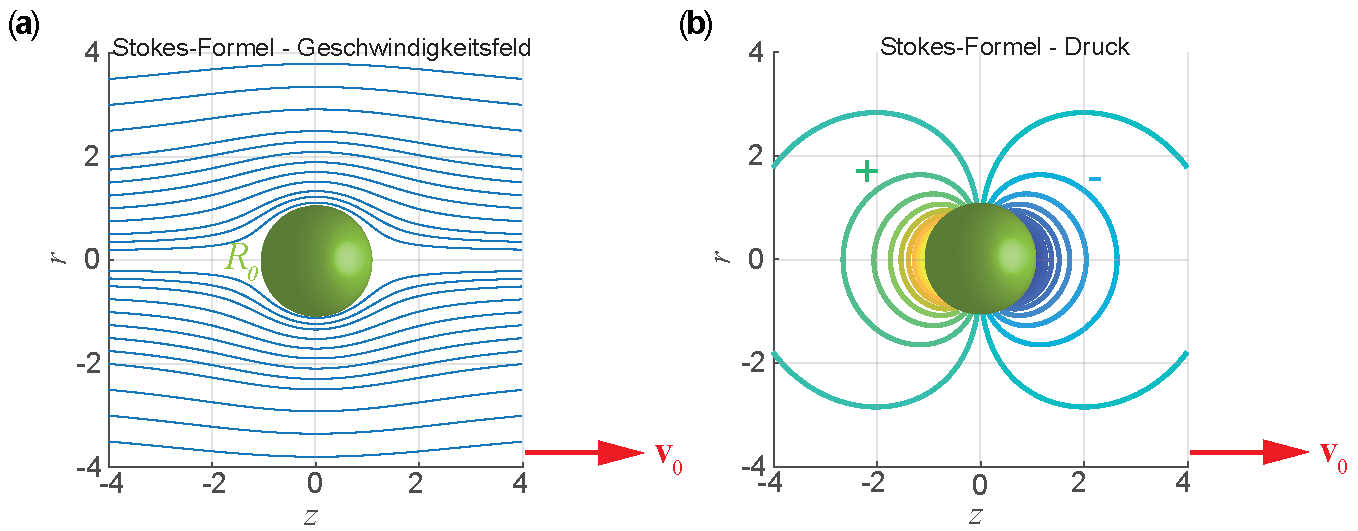
\includegraphics[width=\textwidth]{StokesFormel02.pdf}
    \caption[\fa Geschwindigkeitsprofil und \fb Druck einer viskosen Str�mung um eine Kugel.]
    {Geschwindigkeitsprofil und Druck einer viskosen Str�mung um eine Kugel.}
				\label{abb:kontmech_stokesformel02}
  \end{figure}

Die Auswertung von \eqref{eq:kontmech_Stokes20} ist in \figref{kontmech_stokesformel02} als das Geschwindigkeitsfeld \vec{v}(z,y) dargestellt (siehe auch \mscr{} \mlkontmechref{StokesReibung01.m}).\\

\textbf{Berechnung des Drucks aus dem Geschwindigkeitsfeld}\\

Den Druck kann man aus dem Geschwindigkeitsfeld �ber \eqref{eq:kontmech_Stokes06} aus \eqref{eq:kontmech_Stokes05} berechnen:
\begin{align}     
  \gradv p &= \eta\,\Delta \vec{v} = \eta\,\gradv\lk \Delta\Psi\rk~~\rightarrow~~ p &= p_0 +\eta\,\Delta\Psi \,. \label{eq:kontmech_Stokes21} 
\end{align} 
Wir �berlassen dem Leser die Differentiation, wobei wiederum vorteilhaft die Symbolic Toolbox von \matlab{} benutzt werden kann. Wir geben hier nur das Ergebnis an (siehe auch \figref{kontmech_stokesformel02}).
\begin{align}     
    p &= p_0 - \frac{3}{2}\frac{\eta\,v_0\,R_0\,z}{r^3}\,. \label{eq:kontmech_Stokes_pressure} 
\end{align} 


\textbf{Berechnung der Kraft}\\

Neben dem Druck ben�tigen wir zur Kraftberechnung auch den sogenannten Spannungstensor $\mathbb{T}$. den wir kurz einf�hren wollen (\figref{kontmech_stokesformel03}). Wir k�nnen hier nur eine (f�r den Umfang der �bungsaufgabe hinreichende) Zusammenfassung geben und verweisen den interessierten Leser auf die Literatur, insbesondere \cite{Garvin2023, Schmutzer2005, Bartelmann2015, Hoffmann2000}.

 \begin{figure}
    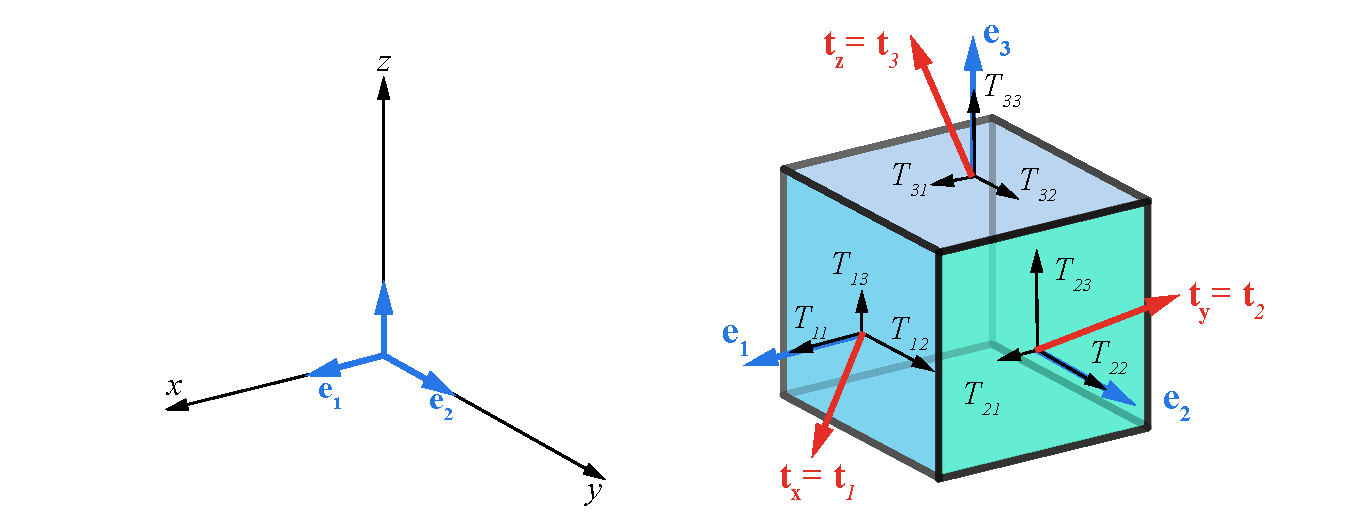
\includegraphics[width=\textwidth]{Spannungstensor.pdf}
    \caption[Komponentendarstellung des Spannungstensors.]
    {Komponentendarstellung des Spannungstensors $T_{ij}$.}
    \label{abb:kontmech_stokesformel03}
  \end{figure}

%Einschub*****************************************************************************************************************

\begin {infobox} {Der Spannungstensor}\index{Spannungstensor}

Bei der Herleitung der 
\begin{itemize}
	\item Euler-Gleichung \eqref{eq:kontmech_EulerGleichung} in \kap{kontmech_EulerGl},
	\item der inneren Reibung in \kap{kontmech_InnereReibung} und daraus folgend der 
	\item der \NVS{} \eqref{eq:kontmech_NavierStokes} in \kap{kontmech_NavierStokes}
\end{itemize}
hatten wir teilweise implizit die Annahme gemacht, dass die Grenzfl�chenkr�fte (auch Spannungsvektoren $\vec{t}_i$ genannt) senkrecht auf den Grenzfl�chen stehen bzw. in der Grenzfl�che liegen (innere Reibung). Wir wollen das nun etwas verallgemeinern und betrachten einen infinitesimal kleinen W�rfel, bei dem jeweils zwei Fl�chen in $x$-, $y$- und $z$-Richtung orientiert sind. Die Orientierung dieser Fl�chen ist gegeben durch den sogenannten Normalenvektor $\vec{e}_\text{n}$, der positiv sein soll, wenn er in Koordinatenrichtung zeigt.
Wir wollen nun zulassen, dass die Spannungsvektoren $\vec{t_x},\, \vec{t_y}$ und $\vec{t_z}$ beliebig zur Fl�che stehen k�nnen (\figref{kontmech_stokesformel03}). Der Spannungstensor $\mathbb{T}$ ist nun die Gr��e, die die Richtung der Kraft mit der Normalenrichtung verkn�pft, also:
\begin{align}     
    \D \vec{F} &= \D A\,\vec{t}\,= \,\D A \,\mathbb{T}\,\vec{e}_\text{n}  ~~~~\text{\bzw}~~~\D \vec{F}_i = \,\D A\, T_{ij}\, e_{\text{n}j} \,. \label{eq:kontmech_Stokes_einschub01} 
\end{align} 
Der Spannungstensor $\mathbb{T}$ \bzw $T_{ij}$ ist ein Tensor zweiter Stufe und fasst die Normalspannungen in Normalenrichtung, sowie tangential wirkende (transversale) Spannungen (auch Scherspannungen genannt) zu einem mathematisch-physikalischen Objekt zusammen. Die Komponenten des Spannungstensors haben die Dimension eines Drucks. Die Komponenten des Spannungstensors k�nnen wir schreiben als.
\begin{align}     
 \mathbb{T}=\left(\vec{t_x},\ \vec{t_y},\ \vec{t_z}\right)=\left(\begin{matrix}T_{xx}&T_{xy}&T_{xz}\\T_{yx}&T_{yy}&T_{yz}\\T_{zx}&T_{zy}&T_{zz}\\\end{matrix}\right) ~~~~\text{\bzw}~~~~~
T_{ij}=\left(\begin{matrix}T_{11}&T_{12}&T_{13}\\T_{21}&T_{22}&T_{23}\\T_{31}&T_{32}&T_{33}\\ \end{matrix}\right) \,.
	\label{eq:kontmech_Stokes_einschub03} 
\end{align}  
%\begin{align}   
%=\left(\begin{matrix}T_{xx}&T_{yx}&T_{zx}\\T_{xy}&T_{yy}&T_{zy}\\T_{xz}&T_{yz}&T_{zz}\\\end{matrix}\right)   
%=\left(\begin{matrix}T_{11}&T_{21}&T_{31}\\T_{12}&T_{22}&T_{32}\\T_{13}&T_{23}&T_{33}\\\end{matrix}\right) 
	%\label{eq:kontmech_Stokes_einschub04} 
%\end{align} 
Die Indizierung der einzelnen Komponenten folgt dabei einem einfachen Schema: Der erste Index $i$ von $T_{ij}$ steht f�r die Richtung der einzelnen Spannungs- \bzw Kraftkomponente. Der zweite Index $j$ steht f�r die Richtung des Normalenvektors. Betrachten wir also $T_{13}$, dann beschreibt dieser Wert die Spannung der $x$-Komponente zur Fl�che, deren Normalenvektor in $z$-Richtung zeigt. Der Tensor ist symmetrisch, \dh $T_{ij} = T_{ji}$, was eine Folge der Drehimpulserhaltung ist \cite{Garvin2023, Schmutzer2005}.\\
Mit dem Spannungstensor schreibt sich die gesamte Fl�chenkraft �ber eine beliebige Oberfl�che
\begin{align}
    \vec{F}_n =  \oint\limits_{\text{Ar}}\,\hat{T}\,\vec{e}_n\,\D A\,, 	\label{eq:kontmech_Stokes_Gesamtkraft} 
\end{align}
woraus mit dem Gau�-Satz folgt:
\begin{align}
    \vec{F}_\text{g} =  \oint\limits_{\text{Ar}}\,\mathbb{T}\,\vec{e}_n\,\D A +\int\limits_{\text{v}_0} \vec{f}_\text{ext} \D V = \int\limits_{\text{v}_0} \divv\,\mathbb{T}\,\D V\, + \vec{f}_\text{V} \,. \label{eq:kontmevh_einschub07}
\end{align}
Wir erhalten somit die allgemeine Bewegungsgleichung f�r ein Fluid  (eigentlich f�r jedes Kontinuum):
\begin{align}     
    \varrho \lk \lk \vec{v} \cdot \nablav \rk \vec{v} + \frac{\partial}{\partial t} \vec{v} \rk \D \vec{F} &= \gradv \cdot \mathbb{T} + \vec{f}_\text{V} \,. 
		\label{eq:kontmech_Cauchy}
\end{align} 
Diese wurde erstmalig von Cauchy\footnote{Augustin-Louis Cauchy (1789--1857) war ein franz�sischer Mathematiker und lieferte fundamentale Beitr�ge zur Analysis und insbesondere auch zur Gruppen- und Funktionentheorie. In der Physik begr�ndete er die modernen Grundlagen der Kontinuumstheorie. Er war in seiner Bedeutung vergleichbar mit dem in Deutschland wirkenden Carl Friedrich Gau�.}\indexp{Cauchy, Augustin-Louis} aufgestellt wurde und besagt, dass die Bewegungs�nderung eines Fluids durch innere und �u�ere Kr�fte hervorgerufen wird, wobei die ersteren sich als Gradient aus dem Spannungstensor ergeben.\footnote{Wir verweisen auf die �hnlichkeit mit der Ableitung der Kraft aus einem Potential f�r die Bewegung eines Massenpunktes.}

%\begin{align}
    %\varrho\,\lek \frac{\d \vec{v}}{\d t} + \lk \vec{v}\,\nablav\,\vec{v}\rek = \vec{f}_\text{ext} + \nablav\,\mathbb{T}\,. 
%\end{align}
Wie ist nun der Spannungstensor aufgebaut? Er besteht aus 3 Anteilen.
\begin{align}
    \mathbb{T} = \mathbb{T}^{\text{(Druck)}} + \mathbb{T}^{\text{(Volumen)}} + \mathbb{T}^{\text{(Viskos)}}\,. \label{eq:kontmech_einschub08}
\end{align}
$\mathbb{T}^{\text{(Druck)}}$ beschreibt die Spannung in einem Fluid, auch wenn dieses keine Bewegung zeigt, das ist genau der Druck:
\begin{align}
    \mathbb{T}^{\text{(Druck)}} = -p\,\mathbb{I} = 
    \begin{pmatrix}
        -p & 0 & 0\\
        0 & -p & 0\\
        0 & 0 & -p
    \end{pmatrix}\,,  \label{eq:kontmech_einschub09}
\end{align}
worin $\mathbb{I}$ der Einheitstensor ist. $\mathbb{T}^{\text{(Volumen)}}$ beschreibt die Spannung in einem Fluid, die durch Volumen�nderung des Fluids entsteht. Logischerweise verschwindet dieser Anteil, wenn die Fl�ssigkeit inkompressibel ist. 
\begin{align}
    \mathbb{T}^{\text{(Volumen)}} = \lambda\,\lk \nablav\,\vec{v}\rk\,\mathbb{I} = 
    \begin{pmatrix}
        \frac{\d v_i}{\d x_i} & 0 & 0\\
        0 & \frac{\d v_i}{\d x_i} & 0\\
        0 & 0 & \frac{\d v_i}{\d x_i}
    \end{pmatrix}\,,  \label{eq:kontmech_einschub09a}
\end{align}
worin wir wieder die Einsteinsche Summenkonvention benutzt haben. Der Proportianalit�tsfaktor $\lambda$ ist die sogenannte Volumenviskosit�t\index{Volumenviskosit�t} oder auch 2. Koeffizient der Viskosit�t genannt. Sie hat die Einheit $\SI{}{\pascal\second}$.\\
Der dritte Term des Spannungstensors beschreibt schlie�lich die durch innere Reibung hervorgerufenen Spannungen. Man k�nnte vermuten nach Behandlung der Reibungskr�fte im \kap{kontmech_InnereReibung}diesen als $\nablav\,\vec{v}$ zu definieren. Dann w�rde der Spannungstensor aber nicht mehr symmetrisch sein, weswegen der viskose Term folgenderma�en definiert wird:
\begin{align}
\begin{split}
    \mathbb{T}^{\text{(Viskos)}} &= \eta\,\lk \nablav\,\vec{v}+\lk\nablav\,\vec{v}\rk^\intercal\rk \\
    &= 
    \begin{pmatrix}
        2\eta\,\frac{\d v_x}{\d x} & \eta\,\lk \frac{\d v_x}{\d x} + \frac{\d v_x}{\d y}\rk & \eta\,\lk \frac{\d v_z}{\d x} + \frac{\d v_x}{\d z}\rk\\
        \eta\,\lk \frac{\d v_x}{\d y} + \frac{\d v_y}{\d x}\rk & 2\eta\,\frac{\d v_y}{\d y} & \eta\,\lk \frac{\d v_z}{\d y} + \frac{d v_y}{\d z}\rk\\
        \eta\,\lk \frac{\d v_x}{\d z} + \frac{\d v_z}{\d x}\rk & \eta\,\lk \frac{\d v_y}{\d z} + \frac{\d v_z}{\d y}\rk & 2\eta\,\frac{\d v_z}{\d z}
    \end{pmatrix}\,,  
\end{split}   \label{eq:kontmech_Stokes_viskoserT} 
\end{align}
$\eta$ ist die dynamische Viskosit�t \bzw der erste Koeffizient der Viskosit�t. Damit kann der Gesamtspannungstensor in Indexschreibweise geschrieben werden als:
\begin{align}
    T_{ij} = -p\,\delta_{ij} + \lambda\,\lk\frac{\d v_k}{\d x_k}\rk\,\delta_{ij} + \eta\,\lk \frac{\d v_i}{\d x_j} + \frac{\d v_j}{\d x_i}\rk\,.\label{eq:kontmech_einschub11a}
\end{align}
F�r inkompressible Fl�ssigkeiten ist $\lambda=0$ und wir erhalten 
\begin{align}
    T_{ij}= -p\,\delta_{ij} + 2\eta\,\lk \frac{1}{2}\,\frac{\d v_i}{\d x_j} + \frac{\d v_j}{\d x_i}\rk\,,\label{eq:kontmech_einschub12}
\end{align}
woraus mit \eqref{eq:kontmech_Cauchy} eingesetzt, die uns bekannte \NVS{} \eqref{eq:kontmech_NavierStokes} aus \kap{kontmech_NavierStokes} folgt. F�r sogenannte Newton-Fl�ssigkeiten gilt \ia der folgende n�herungsweise g�ltige Zusammenhang:
\begin{align}
    \lambda = -\frac{2}{3}\,\eta\,, \label{eq:kontmech_einschub13}
\end{align}
womit wir eine allgemeinere Form der \NVS{} erhalten:
\begin{align}
    \varrho\,\lek \frac{\vec{v}}{\d t} + \lk \vec{v}\,\nablav\rk\,\vec{v}\rek =  \vec{f}_\text{ext} - \nablav\,\lk \frac{2}{3}\,\eta\,\lk \nablav\,\vec{v}\rk\rk + \nablav\,\lk \eta\lk \nablav\,\vec{v}\rk + \lk \nablav\,\vec{v}\rk^\intercal\rk\,. \label{eq:kontmech_einschub14}
\end{align}


\end{infobox}
% Ende Einschub*************************************************************************************** 
\medskip

Zur�ck zur Herleitung der Kraft f�r den Fall einer Kugel in einer viskosen Str�mung. Wir brauchen den nach \eqref{eq:kontmech_Stokes21} berechneten Druck und den viskosen Spannunsgtensor \eqref{eq:kontmech_Stokes_viskoserT}. Dieser lautet in unserem Fall, da wir Inkompressibilit�t und damit $\lambda=0$ voraussetzen: %wegen \eqref{eq:kontmech_Stokes01}
\begin{align}     
  T_{ij}^{\lk \text{visk} \rk} = \eta\,\lk \frac{\d v_{i}}{x_j} +  \frac{\d v_{j}}{x_i} \rk\,. \label{eq:kontmech_Stokes22} 
\end{align} 

Der Gesamtspannungstensor lautet dann
\begin{align}     
T_{ij}  =  T_{ij}^{\lk \text{visk}\rk} + T_{ij}^{\lk \text{p}\rk} = \eta\,\lk \frac{\d v_{i}}{x_j} +  \frac{\d v_{j}}{x_i} \rk - \lk p_0 +\eta\,\Delta\Psi\rk\,\delta_{ij}\,. \label{eq:kontmech_Stokes23} 
\end{align} 
F�r die auf die Kugel wirkende Kraft ergibt sich mit \eqref{eq:kontmech_Stokes_Gesamtkraft} zu:
\begin{align} 
\begin{split}     
   \vec{F}^{\lk \d \text{K}\rk} &= \vec{e}_i F_i^{\lk \d \text{K} \rk} = \vec{e}_i\int\limits_{\d \text{K}} T_{ij} \,\D A_j  = \eta\,\lek \underbrace{\vec{e}_i \int\limits_{\d \text{K} }\,\eta\,\lk \frac{\d v_{i}}{x_j} +  \frac{\d v_{j}}{x_i} \rk\,\D A_j}_{I_1} -\underbrace{\int\limits_{\d \text{K}}\Delta\Psi\,\D\vec{A}}_{I_2}\rek\,. 
		\label{eq:kontmech_Stokes24} 
\end{split} 
\end{align} 
Im folgenden wollen wir die beiden auftretenden Integrale einzeln berechnen, wobei wir die Fl�chenelemente der Kugelfl�che in Polarkoordinaten verwenden:
\begin{align*}     
  \D\vec{A} = \vec{n}\,\D A = \vec{e}_r\,\D A_r ~~ \text{mit} ~~~~\D A_r = R_0{}^2\,\sin\theta\,\D\phi\,\D \theta\,.
\end{align*} 

\begin{enumerate}
\item  [1)] \textbf{Zwischenrechnung f�r Integral} $I_1$\\ 

Wir schreiben: 
\begin{align}
    I_1 = \vec{e}_i \int\limits_{\lk \d \text{K}\rk} \lk \frac{\d v_i}{\d x_j} + \frac{\d v_j}{\d x_i}\rk\,\D A_j = \int\limits_{\lk \d \text{K}\rk} \lk \frac{\d \vec{v}}{d x_j} + \vec{e}_i\,\frac{\d v_j}{\d x_i}\rk \,\D A_j  = \int\limits_{\lk \d \text{K}\rk}\,\lk \frac{\d \vec{v}}{\d r} + \gradv v_r \rk\,\D A_r\,.
\label{eq:kontmech_Stokes25}
\end{align}
Aus dem Geschwindigkeitsfeld \eqref{eq:kontmech_Stokes20} erhalten wir die Beziehungen
\begin{subequations}
\begin{align}
    \vec{v}_0\,\vec{e}_r &= v_0\,\veceZ\,\vec{e}_r = v_0\,\cos\theta\,,\label{eq:kontmech_Stokes26a}\\
    v_r = \vec{v}\,\vec{e}_r &= v_0\,\cos\theta\,\lek 1-\frac{R_0}{2r}\,\lk 3-\frac{R_0{}^2}{r^2}\rk\rek\,.\label{eq:kontmech_Stokes26b}
\end{align}\label{eq:kontmech_Stokes26}
\end{subequations}
F�r die Kugeloberfl�che $\d \text{K}$ berechnet man aus \eqref{eq:kontmech_Stokes20} und \eqref{eq:kontmech_Stokes26b}:
\begin{enumerate}
    \item [a)] \begin{align}
    \frac{\d \vec{v}}{\d r} \,\Big\vert_{r=R_0} &= \frac{3}{2R_0}\,\lek \vec{v}_0 - \vec{0} - \vec{e}_r\,\lk \vec{v}_0\,\vec{e}_r\rk\rek = \frac{3}{2R_0}\,\vec{e}_r \times \lk \vec{v}_0 \times \vec{e}_r\rk = \frac{3}{2R_0} \,\lk \vec{v}_0 - \vec{e}_r\,v_0\,\cos\theta\rk \nonumber \\
    &= \frac{3v_0}{2R_0}\,\lek -\veceX\,\cos\phi\,\sin\theta\,\cos\theta - \veceY\,\sin\phi\,\sin\theta\,\cos\theta + \veceZ\,\sin^2\theta\rek\,\label{eq:kontmech_Stokes27}
\end{align}
    \item [b)] 
    \begin{align}
        \lk\gradv v_r\rk \Big\vert_{r= R_0}  = 0\,.  \label{eq:kontmech_Stokes27a}
    \end{align}
\end{enumerate}
Damit bekommen wir
\begin{align}
    I_2 &= \,\frac{3v_0\,R_0}{2}\int\limits_{\theta=0}^{\pi}\int\limits_{\phi=0}^{2\pi} \left[ -\veceX\,\cos\phi\,\sin^2\theta\,\cos\theta -\veceY\,\sin\phi\,\sin^2\theta\,\cos\theta + \veceZ\,\sin^3\theta\right]\,\D \phi\,\D \theta\,.
 \label{eq:kontmech_Stokes28}
\end{align}
Die Integration �ber $\phi$ ergibt f�r die ersten beiden Glieder des Integranden Nulln. Unter Verwendung einer Integraltafel \cite{Gradshteyn1980} finden wir mit $ \int_0^\pi \sin^3\theta\,\D \theta = 4/3$
aus \eqref{eq:kontmech_Stokes28}
\begin{align}
     I_2 = \frac{3v_0\,R_0}{2}\, 2\pi \veceZ \int_0^\pi \sin^3\theta\,\D \theta = 4\pi\,v_0\,R_0\,\veceZ \,. \label{eq:kontmech_Stokes29}
\end{align}
Der Anteil r�hrt vom viskosen Spannungstensor her und stimmt mit unserer Absch�tzung \eqref{eq:kontmech_kontmech_stokesformel_approx} gut �berein.\\
   
\item  [2)] \textbf{Zwischenrechnung f�r Integral} $I_2$\\

Aus \eqref{eq:kontmech_Stokes09} und \eqref{eq:kontmech_Stokes19} ergibt sich
\begin{align}
\begin{split}
    \int\limits_{\lk \d \text{K}\rk} \Delta\Psi \,\D \vec{A} = &-\frac{3v_0\,R_0}{2}\int\limits_{\theta=0}^{\pi}\int\limits_{\phi=0}^{2\pi}\lk\veceZ\,\vec{e}_r\rk\,\vec{e}_r\,\sin\theta\,\D\theta\,\D\phi\\ \label{eq:kontmech_Stokes30}
    = &-\frac{3v_0\,R_0}{2}\int\limits_{\theta=0}^{\pi}\int\limits_{\phi=0}^{2\pi}\lek \veceX\,\cos\phi\,\sin\theta + \veceY\,\sin\phi\,\sin\theta +\veceZ\,\cos\theta\rek\, \cos\theta\,\sin\theta\,\D\phi\,\D \theta\,.
\end{split}
\end{align}
Auch hier liefern wie oben die ersten beiden Terme des Integranden keinen Beitrag, so dass wir aus dem dritten Term erhalten:
\begin{align}
    \int\limits_{\lk \d \text{K}\rk}\Delta\Psi\,\D\vec{A}= -3\pi\,v_0\,R_0\,\veceZ\int\limits_{\theta=0}^\pi \cos^2\theta\,\sin\theta\,\D \theta = -\int\limits_{\theta=0}^\pi \cos^2\,\D \lk\cos\theta\rk = -\frac{1}{3}\,\cos^3\,\theta\,\Big\vert_0^\pi  = \frac{2}{3}\,.\label{eq:kontmech_Stokes32}
\end{align}
Damit erhalten wir 
\begin{align}
     I_2 = \int\limits_{\lk \d \text{K}\rk}\Delta \Psi \,\D \vec{A}= -2\pi\,v_0\,R_0\,\veceZ\,.\label{eq:kontmech_Stokes33}
\end{align}
Das ist der vom Druckglied herr�hrende Anteil, der in unserer Absch�tzung nicht ber�cksichtigt war.\\
\end{enumerate}

\medskip
\textbf{Zusammenfassung}\\

Die beiden Ergebnisse \eqref{eq:kontmech_Stokes29} und \eqref{eq:kontmech_Stokes33} ergeben zusammen f�r die auf die Kugel wirkende Kraft:
\begin{align}
    \vec{F}^{\lk \d \text{K}\rk} = 6\pi\,\eta\,R_0\,\vec{v}_0 \,, \label{eq:kontmech_Stokes34}
\end{align}
welche verst�ndlicherweise  die Richtung der Geschwindigkeit der Grundstr�mung besitzt. Diese Stokes-Formel gilt wie vorausgesetzt nur bei sehr kleinen Reynolds-Zahlen.\\
Die Stokes-Formel findet Anwendungen in verschiedenen Gebieten der Physik. Erw�hnt sei hier der ber�hmte Millikan\footnote{Robert Andrews Millikan (1868-1953)  war ein US-amerikanischer Experimentalphysiker, der 1923 den Nobelpreis f�r Physik f�r seine ber�hmten �ltr�pfchen-Experimente (Millikan-Versuch) erhielt, mit denen er die Elementarladung eines Elektrons ermittelte.}\indexp{Millikan, Robert Andrews}-Versuch zur Bestimmung der elektrischen Elementarladung durch Messung der Fallgeschwindigkeit elektrisch geladener �ltr�pfchen. \\

\end{sol} 
\textcolor{blue} {$\rightarrow$ zur} \probref{kontmech_StokesReibung}.\\
\noindent\rule[1ex]{\textwidth}{0.5pt}  \newpage  \clearpage

%-----------------------------------------------------------------------------------------------------------
%-----------------------------------------------------------------------------------------------------------

\subsection{�bungen zur Dynamik deformierbarer, fester K�rper}

\medskip


%-----------------------------------------------------------------------------------------------------------


\begin{sol}{prob:kontmech_WelleSaite}\label{lsg:kontmech_WelleSaite} %�bung17
\textbf{Fortschreitende Welle auf der eingespannten Saite}\\ \\

Beide L�sungen lassen sich durch Anpassungen am \matlab{}-Programm
\mlkontmechref{SchwingendeSaite01.m} finden. Diese gehen wir
nacheinander durch.

\begin{enumerate}
\item Wir setzen die Gau�sche St�rung als Anfangsbedingung auf das
  Gitter der Werte $y(x_i,t=0)$. Da die Differentialgleichung von zweiter
  Ordnung in der Zeit ist , muss noch ein zweiter Zeitschritt vorgegeben
  werden. Die St�rung in Form eines Gau�-Pakets soll sich nicht verformen.
  Dies ist m�glich, da die Differentialgleichung \eqref{eq:kontmech_PDGLSaite}
  eine lineare Dispersionsrelation besitzt. Die Anfangsbedingung f�r den
  zweiten Zeitschritt muss jedoch dazu passen. Die Phasengeschwindigkeit
  auf der Saite betr�gt $v_\mathrm{ph} = \sqrt{\kappa/\varrho}$ und
  entsprechend muss das Gau�-Paket im zweiten Zeitschritt um den
  Wert $\sqrt{\kappa/\varrho} \Delta t$ verschoben werden.

  Gibt man dies vor, erh�lt man eine L�sung, wie sie in
  \figref{kontmech_SaiteGausswelle} dargestellt ist. Das Gau�-Paket wandert
  nach rechts, wird dort mit einer Phasenverschiebung von $\pi$ reflektiert
  und kehrt zur�ck.
  
  \begin{figure}
    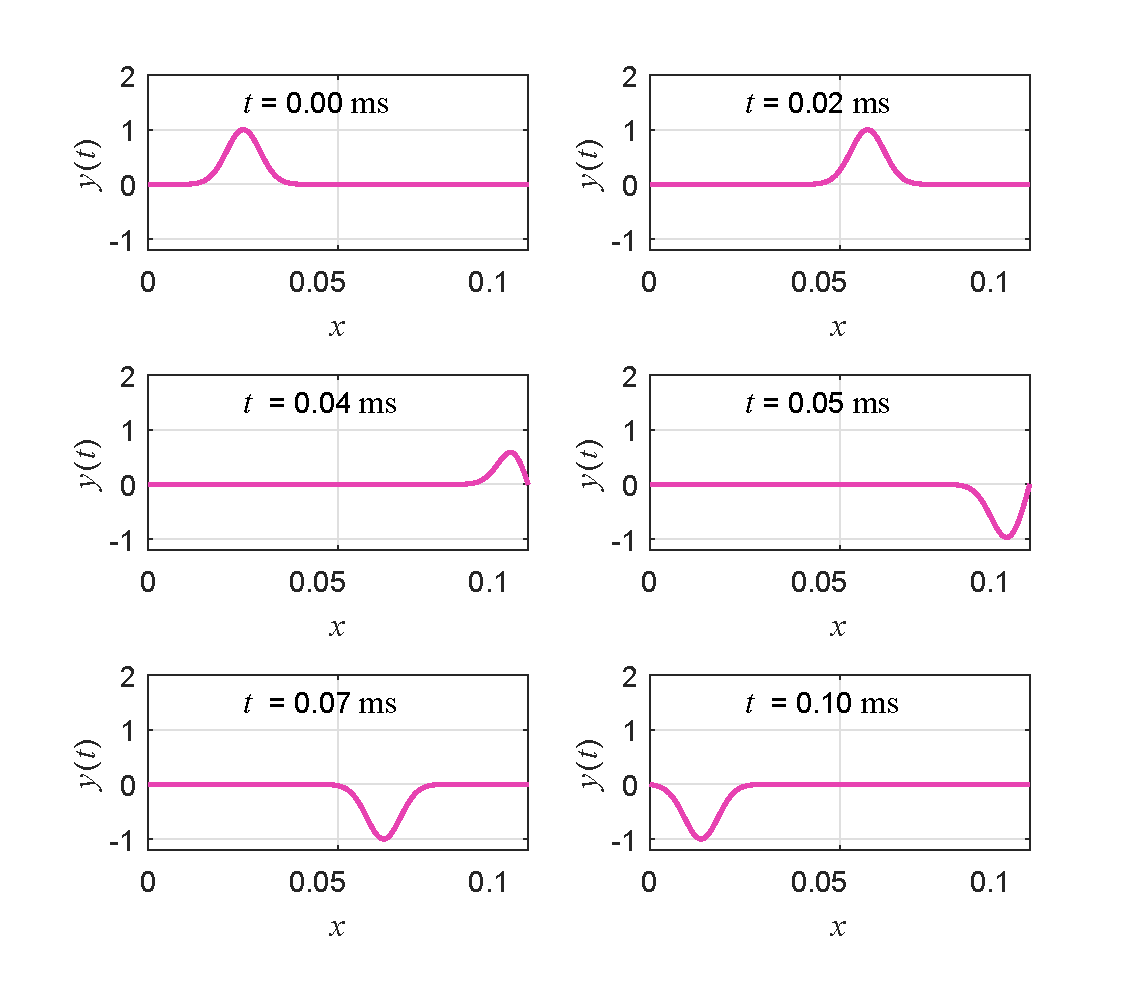
\includegraphics[width=\textwidth]{SchwingendeSaite02.pdf}
    \caption[Gau�sche St�rung auf der eingespannten Saite.]{Eine Gau�sche St�rung
      breitet sich auf der beidseitig eingespannten Saite aus.}
    \label{abb:kontmech_SaiteGausswelle}
  \end{figure}

  \begin{figure}
  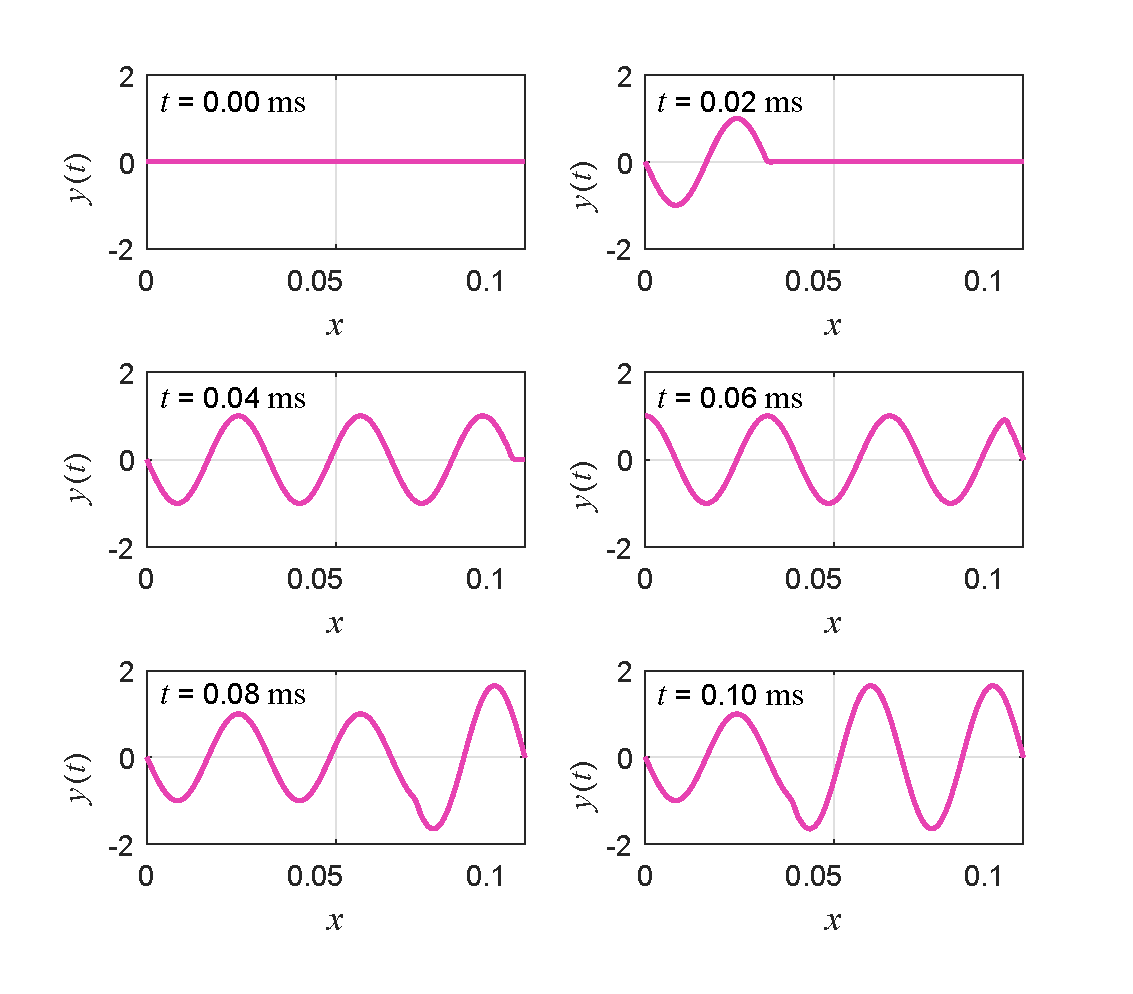
\includegraphics[width=\textwidth]{SchwingendeSaite03.pdf}
  \caption[Angeregte Welle auf der eingespannten Saite.]{Eine Welle wird
    am linken Rand der eingespannten Saite angeregt und am rechten
    Rand reflektiert.}
    \label{abb:kontmech_SaiteAngeregteWelle}
  \end{figure}

\item Im zweiten Fall wird die Anfangsbedingung so gesetzt, dass
  $y(x_i,t=0) = y(x_i,t=\Delta t) = 0$. Einzig der Wert an linken Rand,
  f�r den bisher immer $y(x=0,t_l)= 0$ galt, erh�lt jetzt eine periodische
  Funktion in der Zeit der Form
  \begin{equation*}
    y(x=0,t_l) = \sin \left (\frac{10\,\pi}{T_\mathrm{max}}\, t_l \right ) \;,
  \end{equation*}
  worin $T_\mathrm{max}$ die Ausbreitungszeit �ber die L�nge der Saite ist, \dh die Saite wird mit
	einer Frequenz $5/T_\mathrm{max}$ periodisch am linken Rand angeregt.
	Damit ergibt sich die L�sung aus \figref{kontmech_SaiteAngeregteWelle},
  die eine Welle darstellt, die sich vom linken Rand ausbreitet. Sobald
  sie am rechten Rand ankommt und reflektiert wird, �berlagern sich die
  einlaufende und reflektierte Welle.
  
\end{enumerate}


\end{sol} 
\textcolor{blue} {$\rightarrow$ zur} \probref{kontmech_WelleSaite}.\\
\noindent\rule[1ex]{\textwidth}{0.5pt}  \newpage  \clearpage

%-----------------------------------------------------------------------------------------------------------


\begin{sol}{prob:kontmech_AchterbahnKont}\label{lsg:kontmech_AchterbahnKont} %�bung18
\textbf{Achterbahn-Bewegungsgleichungen im kontinuierlichen Ansatz}\\ \\

Wir starten mit dem Potential nach \eqref{eq:bew_ABdiskret02} aus der
\hyperref[lsg:bew_achterbahn_diskret]{L�sung} zu
\probref{bew_achterbahn_diskret}
\begin{equation*}
  U\lk \{x_i\},\{z_i\}\rk = m\,g\,\sum_{i=1}^{N}z_i + \frac{1}{2}\,k\sum_{i=1}^{N-1}\lk \sqrt{\lk x_{i+1}-x_i\rk^2 + \lk z_{i+1}-z_i\rk^2 }- s_0\rk^2
\end{equation*}
und der kinetischen Energie nach \eqref{eq:bew_ABdiskret02}
\begin{equation}
  T\lk\{\dot{x}_i\},\{\dot{z}_i\}\rk = \frac{1}{2}\,m\sum_{i=1}^{N}\lk \dot{x}_i{}^2 + \dot{z}_i{}^2\rk\,.
  \label{eq:kontmech_AchterbahnGeschw}
\end{equation}
Zun�chst setzen wir hier direkt die Beziehung $z_i=h(x_i)$ ein, um auf die
generalisierte Koordinaten $x_i$ �berzugehen. Dann wird aus den Termen
\begin{equation}
  U\lk \{x_i\}\rk = m\,g\,\sum_{i=1}^{N} h(x_i) + \frac{1}{2}\,k\sum_{i=1}^{N-1}\lk \sqrt{\lk x_{i+1}-x_i\rk^2 + \lk h(x_{i+1})-h(x_i)\rk^2 }- s_0\rk^2
\end{equation}
und der kinetischen Energie nach \eqref{eq:bew_ABdiskret02}
\begin{equation}
  T\lk\{\dot{x}_i\},\{\dot{z}_i\}\rk = \frac{1}{2}\,m\sum_{i=1}^{N}\lk \dot{x}_i{}^2 + \dot{h}(x_i){}^2\rk = \frac{1}{2}\,m\sum_{i=1}^{N}\lk  1 + h'(x_i){}^2 \rk \dot{x}_i{}^2 \,.  
\end{equation}

Die Materiepunkte des Zuges beschreiben wir durch eine Variable $l$ mit
der Eigenschaft $0\leq l \leq L$, wobei $L$ die L�nge des Zuges im
entspannten Zustand auf einer geraden Strecke sein soll. Die tats�chliche
Lage der Materiepunkte im Inertialsystem zu einem beliebigen Zeitpunkt $t$
stellen wir durch die Orte $x(l,t)$ dar.\footnote{Wir wenden also eine
  Beschreibung in Euler-Koordinaten an. Man beachte, dass die Materiepunkte
  unabh�ngig von der aktuellen Lage oder Dehnung des Zuges sich immer auf den
  entspannten Zug auf einer geraden Strecke beziehen und somit die materiellen
  Koordinate $l$ nur Werte zwischen $0$ und $L$ annimmt. Die tats�chliche
  L�nge des Zuges m�ssen wir im Ortsraum bestimmen. Sie ist zu einem
  festen Zeitpunkt $t$ durch $x(L,t)-x(0,t)$ gegeben und kann Werte gr��er
  oder kleiner als $L$ annehmen.}
Um den Kontinuums-Grenzwert vorzubereiten, stellen wir auf:
\begin{subequations}
  \begin{align}
    x_i &\to x(l,t) \\
    s_0 &= \D l \\
    x_{i+1} - x_i &\to \frac{\partial x}{\partial l} \, s_0 =
                          \frac{\partial x}{\partial l} \, \D l\\
    h(x_{i+1}) - h(x_i) &\to \frac{\partial h}{\partial l} \, s_0 = \frac{\partial h}
                          {\partial x} \frac{\partial x}{\partial l} \,s_0
                          = h'(x) \frac{\partial x}{\partial l} \,\D l\\
    m &= \varrho_L \,s_0 = \varrho_L \,\D l \\
    k &= \frac{\Phi}{s_0}
  \end{align}
\end{subequations}
Darin ist $s_0 = \D l$ der Abstand zwischen zwei Wagen in der Ruhelage und
$\varrho_L$ eine L�ngen-Massendichte. Im �bergang vom diskreten Modell zum 
Kontinuum haben wir dann den Kontinuumsgrenzwert f�r $s_0
\to 0$ und $N \to \infty$ bei konstanter Gesamtmasse $M = \varrho_\text{L}\,L$ des Zuges zu bilden.

Mit diesen Definitionen formen wir zun�chst das Potential um. F�r dieses
finden wir
\begin{subequations}
  \begin{align}
    U\lk \{x_i\}\rk
    &= m\,g\,\sum_{i=1}^{N} h(x_i) + \frac{1}{2}\,k\sum_{i=1}^{N-1} \lk
      \sqrt{\lk x_{i+1}-x_i\rk^2 + \lk h(x_{i+1})-h(x_i) \rk^2 }- s_0\rk^2
      \notag \\
    &=  \varrho_L\,g\,\sum_{i=1}^{N} h(x_i) s_0 + \frac{1}{2}\,k\sum_{i=1}^{N-1} \lk
      \sqrt{\lk \frac{\partial x}{\partial l} s_0 \rk^2 + \lk h'(x)
      \frac{\partial x}{\partial l} \,s_0 \rk^2 }- s_0\rk^2 \notag \\
    &=  \varrho_L\,g\,\sum_{i=1}^{N} h(x_i) s_0 + \frac{1}{2}\,k\sum_{i=1}^{N-1}
      \lk \sqrt{1 + h'(x)^2 }\, \frac{\partial x}{\partial l} \, s_0 - s_0\rk^2
      \notag \\
    &=  \varrho_L\,g\,\sum_{i=1}^{N} h(x_i) s_0 + \frac{1}{2}\,k\sum_{i=1}^{N-1}
      \lk \sqrt{1 + h'(x)^2 }\, \frac{\partial x}{\partial l} \, - 1\rk^2 s_0^2
      \notag \\
    &=  \varrho_L\,g\,\sum_{i=1}^{N} h(x_i) s_0 + \frac{1}{2}\,\Phi\,
      \sum_{i=1}^{N-1} \lk \sqrt{1 + h'(x)^2 }\, \frac{\partial x}{\partial l}
      \, - 1\rk^2 s_0
  \end{align}
  Im Grenzwert $s_0 = \D l \to 0$, $N\to\infty$ erkennen wir darin zweimal das
  Riemann\footnote{Georg Friedrich Bernhard Riemann\indexp{Riemann, Georg Friedrich Bernhard} (1826--1866) war ein deutscher Mathematiker, der trotz seines relativ kurzen Lebens als einer der bedeutendsten Mathematiker gilt. Er arbeitete unter anderem bahnbrechend auf den Gebieten der Analysis, Differentialgeometrie und der mathematischen Physik.}-Integral\footnote{Das Riemann-Integral l�sst sich �ber die anschauliche Vorstellung des Integrals als Fl�cheninhalt zwischen der $x$-Achse und dem Graphen einer Funktion definieren. Die zugrundeliegende Idee besteht darin, den gesuchten Fl�cheninhalt mit Hilfe des leicht zu berechnenden Fl�cheninhalts von Rechtecken anzun�hern, \zb von von sogenannten "`Obersummen"' und "`Untersummen"' von Rechtecken, die so gebildet werden, dass der Funktionsgraph zwischen diesen liegt. Indem man  die Anzahl der Rechtecke gegen $\infty$ gehen l�sst, erh�lt man eine immer genauere Approximation des Fl�cheninhalts zwischen dem Funktionsgraphen und der $x$-Achse \cite{Arens2008}.}, was uns f�r einen Zug der L�nge $L$ auf
  \begin{equation}
    U\lk x , \frac{\partial x}{\partial l}\rk =
    \int_{0}^{L} \left \{ \varrho_L\,g\, h(x(l)) + \frac{1}{2}\,\Phi\,
      \lk \sqrt{1 + h'(x(l))^2}\, \frac{\partial x(l)}{\partial l} \, - 1\rk^2
      \right \} \, \D l
    \end{equation}
    f�hrt.
\end{subequations}
Analog finden wir im selben Grenzwert f�r die kinetische Energie
\begin{align}
  T\lk x , \frac{\partial x}{\partial t} \rk
  &= \frac{1}{2}\,m\sum_{i=1}^{N}\lk  1 + h'(x_i){}^2 \rk \dot{x}_i{}^2
  = \frac{1}{2}\,\varrho_L \sum_{i=1}^{N}\lk  1 + h'(x_i){}^2 \rk \dot{x}_i{}^2
  \, s_0 \notag \\
  &= \int_{0}^{L} \frac{1}{2}\,\varrho_L \lk  1 + h'(x(l)){}^2 \rk
    \lk \frac{\partial x}{\partial t} \rk^2 \, \D l \; .
\end{align}
Zusammengef�gt ergibt sich die Lagrange-Funktion
\begin{subequations}
  \begin{equation}
    \mathcal{L} \lk x , \frac{\partial x}{\partial t} , \frac{\partial x}{\partial l} \rk
     = \int_{0}^{L} L \lk x , \frac{\partial x}{\partial t} , \frac{\partial x}{\partial l} \rk \, \D l
  \end{equation}
  mit der Lagrange-Dichte
  \begin{multline}
    L \lk x , \frac{\partial x}{\partial t} , \frac{\partial x}{\partial l} \rk
    = \frac{1}{2}\,\varrho_L \lk  1 + h'(x(l)){}^2 \rk \lk \frac{\partial x}
    {\partial t} \rk^2 \\
    - \varrho_L\,g\, h(x(l)) - \frac{1}{2}\,\Phi\, \lk \sqrt{1 + h'(x(l))^2}
    \, \frac{\partial x(l)}{\partial l} \, - 1\rk^2 \,. \label{eq:kontmech_AchterbahnKont07}
  \end{multline}
\end{subequations}

Wir vergleichen \eqref{eq:kontmech_AchterbahnKont07} mit der
Lagrange-Funktion $\mathcal{L}$ aus \kap{bew_lagrange_formalism} f�r
Massepunkte. Offensichtlich hat im Kontinuumsfall die Lagrange-Dichte
noch eine zus�tzliche unabh�ngige Variable $x' = \partial x / \partial l$, die
wir bereits bei der schwingenden Saite (Beispiel
\ref{bsp:kontmech_schwingendeSaite}) kennen gelernt und ber�cksichtigt hatten. 
Im Unterschied zur schwingenden Saite h�ngt hier nun die Lagrange-Dichte
nicht nur von $\partial x/\partial l$ und $\partial x/\partial t$ ab, sondern
auch noch explizit von $x$. Dies l�sst sich jedoch leicht ber�cksichtigen und 
stellt kein Problem f�r die Variationsrechnung\footnote{Zur Erinnerung: In der
  Variationsrechnung werden die Positionen $x(l)$, die Geschwindigkeiten
  $\dot{x}(l)=\partial x/\partial t$ und die Dehnung $x'(l)=\partial x/
  \partial l$ variiert, wobei die Gesamtl�nge $L$ und die Gesamtzeit der
  Bewegung $T$ konstant bleibt.} dar, mit der wir die Bewegungsgleichung
ableiten wollen. Wir stellen das Wirkungsfunktional
\begin{subequations}
  \allowdisplaybreaks
  \begin{equation}
    S =  \int \D t\, \int_{0}^{L} \D l \, L \lk x , \frac{\partial x}
    {\partial l} , \frac{\partial x}{\partial t} \rk  = \int \D t\, \int_{0}^{L} \D l \, L \lk x , \dot{x}, x' \rk 
  \end{equation}
  auf und f�hren dessen Variation ein,
  \begin{align}
    \delta S &= \int_0^T \D t\, \int_{0}^{L} \D l \, \left \{ L \lk x
               + \delta x ,
               \frac{\partial x}{\partial l} + \frac{\partial \delta x}
               {\partial l},
               \frac{\partial x}{\partial t} + \frac{\partial \delta x}
               {\partial t}
               \rk
               - L \lk x , \frac{\partial x}{\partial l} , \frac{\partial x}
               {\partial t}\rk \right \} \notag \\
             &\overset{\text{Linearisierung}}{\approx}
               \int_0^T \D t\, \int_{0}^{L} \D l \, \left \{
               L \lk x, \frac{\partial x}{\partial l}, \frac{\partial x}
               {\partial t} \rk
               + \frac{\partial L}{\partial x} \, \delta x
               + \frac{\partial L}{\partial \frac{\partial x}{\partial l}}
               \frac{\partial \delta x}{\partial l}
               + \frac{\partial L}{\partial \frac{\partial x}{\partial t}}
               \frac{\partial \delta x}{\partial t}
               - L \lk x , \frac{\partial x}{\partial l} , \frac{\partial x}
               {\partial t}\rk \right \} \notag \\
             &= \int_0^T \D t\, \int_{0}^{L} \D l \, \left \{
               \frac{\partial{L}}
               {\partial x}\,\delta x + \frac{\partial L}{\partial
               \frac{\partial x}{\partial l}} \,  \frac{\partial \delta x}
               {\partial l} + \frac{\partial L}{\partial
               \frac{\partial x}{\partial t}} \,  \frac{\partial \delta x}
               {\partial t} \right \} \notag \\
             &\underset{\text{zweiter Term}}{\overset{\text{part. Int.}}{=}}
               \underbrace{\lek \frac{\partial L}{\partial\frac{\partial x}
               {\partial l}}\, \delta x \rek_0^L}_{=0}
               + \int_0^T \D t\, \int_{0}^{L} \D l \, \left \{
               \frac{\partial{L}}{\partial x}\,\delta x
               - \lk \frac{\partial}{\partial l} \frac{\partial L}
               {\partial\frac{\partial x}{\partial l}} \rk \delta x
               + \frac{\partial L}{\partial \frac{\partial x}{\partial t}}
               \,  \frac{\partial \delta x}{\partial t} \right \} \notag \\
             &\underset{\text{dritter Term}}{\overset{\text{part. Int.}}{=}}
               \underbrace{\lek \frac{\partial L}{\partial\frac{\partial x}
               {\partial t}}\, \delta x \rek_0^T}_{=0}
               + \int_0^T \D t\, \int_{0}^{L} \D l \, \left \{
               \frac{\partial{L}}{\partial x}\,\delta x
               - \lk \frac{\partial}{\partial l} \frac{\partial L}
               {\partial\frac{\partial x}{\partial l}} \rk \delta x
               - \lk \frac{\partial}{\partial t} \frac{\partial L}
               {\partial \frac{\partial x}{\partial t}} \rk \delta x
               \right \} \notag \\
             &= \int_0^T \D t\, \int_{0}^{L} \D l \, \left \{
               \frac{\partial{L}}{\partial x}
               - \frac{\partial}{\partial l} \frac{\partial L}{\partial
               \frac{\partial x}{\partial l}}
               - \frac{\partial}{\partial t} \frac{\partial L}{\partial
               \frac{\partial x}{\partial t}}
               \right \}  \, \delta x \; .
  \end{align}
\end{subequations}
Die Randterme liefern in der partiellen Integration keinen Beitrag, da die
Variation $\delta x$ definitionsgem�� am Rand verschwindet. Die sie aber
ansonsten beliebig ist, lesen wir die notwendige Bedingung
\begin{equation}
  \frac{\partial{L}}{\partial x}
  - \frac{\partial}{\partial t} \frac{\partial L}{\partial
    \frac{\partial x}{\partial t}}
	- \frac{\partial}{\partial l} \frac{\partial L}{\partial
    \frac{\partial x}{\partial l}}=
  \frac{\partial{L}}{\partial x}
  - \frac{\partial}{\partial t} \frac{\partial L}{\partial \dot{x}} 
  - \frac{\partial}{\partial l} \frac{\partial L}{\partial x'} =0
  \label{eq:kontmech_AchterbahnLagrangeDGL}
\end{equation}         
ab. 

Zum Aufstellen der Bewegungsgleichungen m�ssen wir die entsprechenden
Ableitungen bilden. Diese sind:
\begin{subequations}
  \allowdisplaybreaks
  \begin{align}
    \frac{\partial{L}}{\partial x} &= \varrho_L h'(x)h''\frac{\partial L}{\partial\frac{\partial x}{\partial l}} - \varrho_L g h'(x)
                                     - \Phi \lk \sqrt{1 + h'(x)^2}\, \frac{\partial x}{\partial l} - 1 \rk \frac{h'(x)h''(x)} {\sqrt{1 + h'(x)^2}} \,\frac{\partial x}
                                     {\partial l} \, \notag \\
                                   &= \varrho_L h'(x)h''(x) \lk \frac{\partial x}{\partial t} \rk^2 - \varrho_L g h'(x) -\Phi\, h'(x)h''(x) \lk \frac{\partial x}{\partial l} \rk^2 + \Phi\, \frac{h'(x)h''(x)}{\sqrt{1 + h'(x)^2}}\,\frac{\partial x}{\partial l} \\
    \frac{\partial{L}}{\partial \frac{\partial x}{\partial l}} &=- \Phi\, \lk \sqrt{1 + h'(x)^2}\, \frac{\partial x}{\partial l} \,
                                                                 - 1 \rk \sqrt{1 + h'(x)^2} =- \Phi\,\lk \lk \sqrt{1 + h'(x)^2} \rk\, \frac{\partial x}{\partial l} - \sqrt{1 + h'(x)^2} \rk  \\
    \frac{\partial}{\partial l}\frac{\partial L}{\partial\frac{\partial x}{\partial l}} &= - 2 \Phi\, h'(x)h''(x) \, \lk \frac{\partial x}{\partial l} \rk^2 - \Phi\, \lk 1 + h'(x)^2 \rk \frac{\partial^2 x}{\partial l^2} + \Phi\, \frac{h'(x)h''(x)}{\sqrt{1 + h'(x)^2}} \, \frac{\partial x}{\partial l} \\
    \frac{\partial L}{\partial\frac{\partial x}{\partial t}} &= \varrho_L \lk  1 + h'(x){}^2 \rk \frac{\partial x}{\partial t} \\
    \frac{\partial}{\partial t} \frac{\partial L}{\partial\frac{\partial x}{\partial t}} &= 2 \varrho_L \, h'(x)h''(x) \lk \frac{\partial x}{\partial t} \rk^2 + \varrho_L \lk  1 + h'(x){}^2 \rk \frac{\partial^2 x}{\partial t^2}\,.
  \end{align}
\end{subequations}

Dies fasst man in der Bewegungsgleichung
\eqref{eq:kontmech_AchterbahnLagrangeDGL} zusammen zu
\begin{subequations}
  \begin{multline}
    -\varrho_L h'(x)h''(x) \lk \frac{\partial x}{\partial t} \rk^2
    - \varrho_L g h'(x)
    +\Phi\, h'(x)h''(x) \lk \frac{\partial x}{\partial l} \rk^2 \\
    + \Phi\, \lk 1 + h'(x)^2 \rk \frac{\partial^2 x}{\partial l^2}
    - \varrho_L \lk  1 + h'(x){}^2 \rk \frac{\partial^2 x}{\partial t^2}
    = 0 \; ,
  \end{multline}
  was noch nach
  \begin{equation}
    \frac{\partial^2 x}{\partial t^2} = -\frac{h'(x)h''(x)}{1 + h'(x){}^2}
    \lk \frac{\partial x}{\partial t} \rk^2
    - \frac{g h'(x)}{1 + h'(x){}^2}
    +\frac{\Phi}{\varrho_L}\, \frac{h'(x)h''(x)}{1 + h'(x){}^2} \lk
    \frac{\partial x}{\partial l} \rk^2
    + \frac{\Phi}{\varrho_L}\, \frac{\partial^2 x}{\partial l^2}
    \label{eq:kontmech_DGLkontAchterbahn}
  \end{equation}
  aufgel�st werden kann.


  Man beachte insbesondere, dass f�r einen
  starren Zug, der seine L�nge nicht ver�ndern kann, f�r den also
  \begin{equation*}
    x' = \frac{\partial x}{\partial l} = x'' = \frac{\partial^2 x}{\partial l^2}
    = 0
  \end{equation*}
  gilt, die Bewegungsgleichung \eqref{eq:kontmech_DGLkontAchterbahn}
  die Form
  \begin{equation*}
    \ddot{x} = - \frac{h'(x)h''(x)}{1 + h'(x){}^2}\dot{x}^2
    - \frac{g h'(x)}{1 + h'(x){}^2}
  \end{equation*}
  annimmt, die wir schon aus der \hyperref[lsg:bew_achterbahn]{L�sung}
  zu \probref{bew_achterbahn} (vgl. mit den Gleichungen
  \eqref{eq:bew_Achterbahn03} und \eqref{eq:bew_Achterbahn05}) kennen.
\end{subequations}
  
\end{sol} 
\textcolor{blue} {$\rightarrow$ zur} \probref{kontmech_AchterbahnKont}.\\
\noindent\rule[1ex]{\textwidth}{0.5pt}  \newpage  \clearpage

%-----------------------------------------------------------------------------------------------------------

\begin{sol}{prob:kontmech_AchterbahnZug}\label{lsg:kontmech_AchterbahnZug} %�bung19
\textbf{Elastischer Achterbahnzug auf einer Gau�kurven-Strecke}\\ \\

Analog zum Vorgehen bei der schwingenden Saite in Beispiel
\ref{bsp:kontmech_finiteDiffSaite} diskretisieren wir die Bewegungsgleichung.
F�r die erste und zweite Ableitung von $x$ nach der Zeit schreiben wir
\begin{align*}
  \frac{\partial x}{\partial t}
  &\to \frac{x(l_i,t_{j}) - x(l_i,t_{j-1})}{\Delta t} \; ,\\
  \frac{\partial^2 x}{\partial t^2}
  &\to \frac{x(l_i,t_{j+1}) + x(l_i,t_{j-1}) -2 x(l_{i},t_{j})}{\Delta t^2}
    \; .
\end{align*}
Analog bilden wir f�r die Ableitung nach der materiellen Koordinate $l$
\begin{align*}
  \frac{\partial x}{\partial l}
  &\to \frac{x(l_i,t_j) - x(l_{i-1},t_j)}{\Delta l} \; ,\\
  \frac{\partial^2 x}{\partial l^2}
  &\to \frac{x(l_{i+1},t_j) + x(l_{i-1},t_j) -2 x(l_{i},t_{j})}{\Delta t^2}
    \; .
\end{align*}
Eingesetzt in die Differentialgleichung erh�lt man
\begin{align}
\begin{split}
  \frac{x(l_i,t_{j+1}) + x(l_i,t_{j-1}) -2 x(l_{i},t_{j})}{\Delta t^2}
  = -\frac{h'(x)h''(x)}{1+h'(x)^2} \lk \frac{x(l_i,t_{j}) - x(l_i,t_{j-1})}
  {\Delta t} \rk^2 \\
  - g \frac{h'(x)}{1+h'(x)^2}
  + \frac{\Phi}{\varrho_L} \frac{h'(x)h''(x)}{1+h'(x)^2}
  \lk \frac{x(l_i,t_j) - x(l_{i-1},t_j)}{\Delta l} \rk^2 \\
  + \frac{\Phi}{\varrho_L} \frac{x(l_{i+1},t_j) + x(l_{i-1},t_j)
    -2 x(l_{i},t_{j})}{\Delta t^2} \; .  
\end{split} \label{eq:kontmech_DGLkontAchterbahn02}
\end{align}
Dies f�hrt auf die Iterationsgleichung in der Zeit:
\begin{align}
\begin{split}
  x(l_i,t_{j+1}) = 2 x(l_{i},t_{j}) - x(l_i,t_{j-1}) 
  - \frac{h'(x)h''(x)}{1+h'(x)^2} \lk x(l_i,t_{j}) - x(l_i,t_{j-1}) \rk^2 \\
  - g \frac{h'(x)}{1+h'(x)^2} \Delta t^2
  + \frac{\Phi}{\varrho_L} \frac{h'(x)h''(x)}{1+h'(x)^2} \lk \frac{\Delta t}
  {\Delta l} \rk^2 \lk x(l_i,t_j) - x(l_{i-1},t_j) \rk^2 \\
  + \frac{\Phi}{\varrho_L} \lk \frac{\Delta t}
  {\Delta l} \rk^2 \lk x(l_{i+1},t_j) + x(l_{i-1},t_j)
  -2 x(l_{i},t_{j}) \rk
\end{split} \label{eq:kontmech_DGLkontAchterbahn03}
\end{align}
Eine numerische L�sung dieser Gleichung mithilfe der \matlab{}-Datei
\mlkontmechref{AchterbahnKont.m} ist in
\figref{kontmech_AchterbahnKont} dargestellt. Der Zug startet
in diesem Programm zur Zeit $t=0$ weit weg von der Gau�kurvenstrecke und
f�hrt auf diese zu. 
\begin{figure}
  \centering
  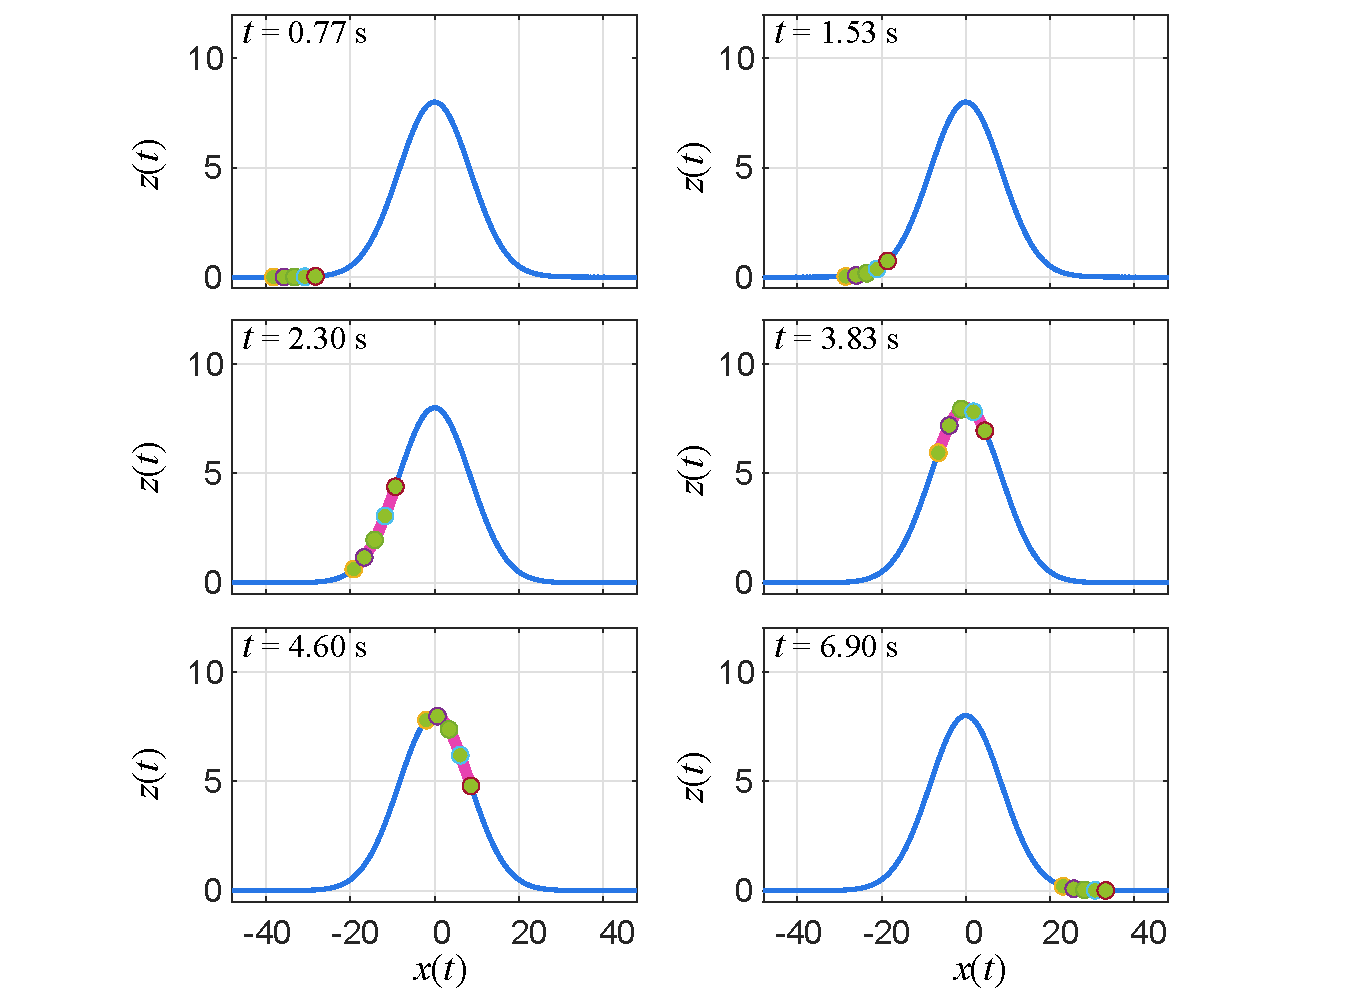
\includegraphics[width=\textwidth]{AchterbahnKont.pdf}
  \caption[Elastischer Achterbahnzug auf der Gau�kurvenstrecke.]
  {Elastischer Achterbahnzug zu verschiedenen Zeitpunkten auf der
    Gau�kurvenstrecke. Die gr�nen Punkte entsprechen materiellen Koordinaten
    in �quidistanten Abst�nden.}
  \label{abb:kontmech_AchterbahnKont}
\end{figure}
In der Berechnung des diskreten Systems eines Zuges aus Wagen, die mit
Federn gekoppelt sind, in der \hyperref[lsg:bew_achterbahn_diskret]{L�sung} zu
\probref{bew_achterbahn_diskret} hat sich bereits gezeigt, dass der Abstand
zwischen den ersten beiden Wagen zun�chst sinkt, wenn der erste Wagen in
die Steigung der Gau�kurvenstrecke f�hrt, und anschlie�end steigt, wenn die
Feder gegen die Bewegung dr�ckt und immer weitere Teile des Zuges gegen
die Gravitation ank�mpfen m�ssen. Dies ist von einer Schwingung durch
die Federn �berlagert. In \figref{kontmech_KreisRohrGeschwindigkeit} ist
etwas �hnliches zu erkennen. Die gr�nen Punkte markieren Punkte mit
konstantem Abstand der materiellen Koordinaten. F�r einen ruhenden, entspannten
Zug sind auch ihre r�umlichen Abst�nde konstant. W�hrend dies kurz vor dem
Erreichen der Gau�kurvenstrecke noch der Fall ist, sieht man wie zu $t=
\SI{1.53}{\second}$ der Abstand zwischen den ersten beiden Wagen steigt. Dies
verst�rkt sich f�r alle Wagen zur Zeit $t=\SI{2.30}{\second}$.

Um die Spitze des Berges herum verdichten sich die Punkte, nach deren
�berwinden steigen die Abst�nde wieder. Auch das hat sich im diskreten Modell
so gezeigt. Mit zunehmender Beschleunigung der hinteren Zugteile, w�hrend der
vordere bereits wieder auf flacheren Streckenteilen unterwegs ist, verk�rzen
sich die Abst�nde nach vorne. Nach �berwinden des Gau�-Berges finden noch
Schwingungsbewegungen des elastischen Zuges statt. Das hei�t, der Zug kehrt
nicht zu seiner reinen Schwerpunktsbewegung zur�ck, die er vor der Gau�kurve
hatte. Ein Teil der Energie wurde in die Relativbewegung der einzelnen
Zugteile gegeneinander transferiert. Diesen Effekt konnte man bereits
im diskreten Modell sehen (vgl.\ \hyperref[lsg:bew_achterbahn_diskret]{L�sung}
zu \probref{bew_achterbahn_diskret}). In einem realen Zug w�rden nat�rlich
sowohl die Relativ- als auch die Schwerpunktsbewegung ged�mpft werden, sodass der
Zug am Ende wieder die urspr�ngliche, entspannte Form annehmen w�rde, aber
auch langsamer w�re als am Beginn der Kurve.

\end{sol} 
\textcolor{blue} {$\rightarrow$ zur} \probref{kontmech_AchterbahnZug}.\\
\noindent\rule[1ex]{\textwidth}{0.5pt}  \newpage  \clearpage

%-----------------------------------------------------------------------------------------------------------

\begin{sol}{prob:kontmech_AchterbahnBeschleunigungen}\label{lsg:kontmech_AchterbahnBeschleunigungen} %�bung20
\textbf{Normalbeschleunigung eines Fahrgastes im Achterbahnzug}\\ \\

Jeder Fahrgast sp�rt in jedem Fall seine Gewichtskraft, die zu einer
Fallbeschleunigung $-g\veceZ$ f�hrt. Dar�ber hinaus folgt er der
Bewegung des Wagens und sp�rt die Radialbeschleunigung der nicht-geradlinigen
Bewegung. Die $x$-Komponente kann prinzipiell aus der Bewegungsgleichung
\eqref{eq:kontmech_DGLkontAchterbahn} extrahiert werden. Wir wollen
hier jedoch die Normalkomponenten mit einer eigenen Betrachtung finden.

Die Radialbeschleunigung hat den Betrag
\begin{equation}
  a_r = \frac{v^2}{r}
\end{equation}
mit der Geschwindigkeit $v$ entlang der Bahn und dem Radius $r$ des Kreises,
der an der Bahn anliegt und deren Kr�mmung im entsprechenden Bahnpunkt
wiedergibt. Die Geschwindigkeit $v$ erhalten wir direkt aus der numerischen
L�sung des Bahnverlaufs.
Um $r$ zu bestimmen, suchen wir erst den Kreis, der an der Bahn anliegt und
dessen Funktion $z(x)$ die Kr�mmung der Bahn richtig wiedergibt, siehe
\figref{kontmech_KreisAnliegend}.

\begin{figure}
  \centering
  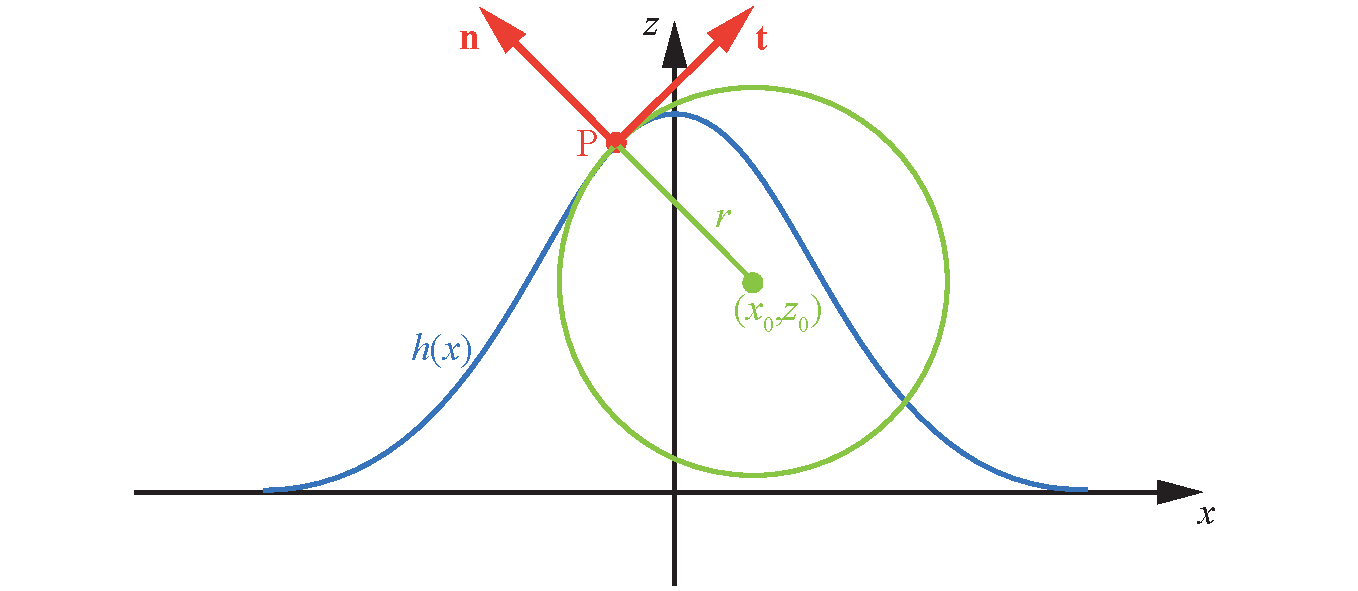
\includegraphics[width=\textwidth]{AchterBahnKreis.pdf}
  \caption[Kreis zur Bestimmung der Radialbeschleunigung.]
  {Kreis, der an die Achterbahnkurve anliegt und die Kr�mmung am Punkt
    P korrekt beschreibt, um daraus die Radialbeschleunigung zu bestimmen.}
  \label{abb:kontmech_KreisAnliegend}
\end{figure}

Zur Berechnung l�sen wir die Kreisgleichung
\begin{subequations}
  \begin{equation}
    (x-x_0)^2 + (z-z_0)^2 = r^2
  \end{equation}
  nach 
  \begin{equation}
    z(x) = \pm \sqrt {r^2 - (x-x_0)^2 }
  \end{equation}
\end{subequations}
auf. Um die richtige Steigung f�r das Anliegen und die richtige Kr�mmung
bestimmen zu k�nnen, ben�tigen wir die erste und die zweite Ableitung. Beide
m�ssen anschlie�end mit der Bahn �bereinstimmen. Die erste Ableitung
f�hrt auf
\begin{subequations}
  \begin{equation}
    \frac{\D z}{\D x} = \mp \frac{x-x_0}{\sqrt {r^2 - (x-x_0)^2 }}
    = - \frac{x-x_0}{z-z_0}
  \end{equation}
  und damit erhalten wir
  \begin{multline}
    \frac{\D^2 z}{\D x^2} = \frac{\D}{\D x} \lk - \frac{x-x_0}{z-z_0} \rk
    = - \frac{x-x_0}{z-z_0} = - \frac{1}{z-z_0} + \frac{x-x_0}{(z-z_0)^2}
    \frac{\D z}{\D x} \\
    = - \frac{1}{z-z_0} - \frac{1}{(z-z_0)} \lk \frac{\D z}{\D x} \rk^2 
    = - \frac{1}{z-z_0} \lk 1 + \lk \frac{\D z}{\D x} \rk^2 \rk
  \end{multline}
\end{subequations}

Damit der Kreis wie gew�nscht an der Kurve anliegt, m�ssen die drei
Gleichungen
\begin{subequations}
  \begin{align}
    z(x) &= \pm \sqrt {r^2 - (x-x_0)^2 } \overset{!}{=} h(x) \\
    \frac{\D z}{\D x} &= - \frac{x-x_0}{z-z_0} \overset{!}{=} h'(x) \\
    \frac{\D^2 z}{\D x} &= - \frac{1}{z-z_0} \lk 1 + \lk \frac{\D z}{\D x}
                          \rk^2 \rk = - \frac{1}{z-z_0} \lk 1 + h'(x)^2
                          \rk \overset{!}{=} h''(x)
  \end{align}
\end{subequations}
erf�llt sein. Die letzte Gleichung l�sst sich zu
\begin{subequations}
  \begin{equation}
   z-z_0 = \frac{1+h'^2}{h''}
 \end{equation}
 aufl�sen, was mit der zweiten auf
  \begin{equation}
   x-x_0 = - \frac{1+h'^2}{h''} h'
 \end{equation}
 f�hrt und schlie�lich mit der ersten zur Bestimmung des Radius nach
 \begin{equation}
   r = \frac{1+h'^2}{h''} \sqrt{1+h'^2}
 \end{equation}
\end{subequations}
herangezogen werden kann.

Mit dem Geschwindigkeitsquadrat nach \eqref{eq:kontmech_AchterbahnGeschw}
\begin{equation}
  v^2 = (1+h'^2) \dot{x}^2
\end{equation}
ergibt sich die Radialbeschleunigung zu
\begin{equation}
  a_r = \frac{h''}{1+h'^2}\sqrt{1+h'^2}\, \dot{x}^2 \; .
\end{equation}
Um ihr eine Richtung zu geben, f�hren wir den normierten Tangentialvektor an
die Achterbahnkurve (siehe \figref{kontmech_KreisAnliegend})
\begin{subequations}
  \begin{equation}
    \vec{t} = \frac{1}{\sqrt{\D x^2 + \D z^2}} \begin{pmatrix} \D x \\
      \D z \end{pmatrix}
    = \frac{1}{\sqrt{(1 + h'(x)^2) \D x^2}} \begin{pmatrix} \D x \\
      h'(x) \D x \end{pmatrix}
    =  \frac{1}{\sqrt{1 + h'(x)^2}} \begin{pmatrix} 1 \\
      h'(x)  \end{pmatrix}
  \end{equation}
  ein und bilden den dazu Normalenvektor, der immer nach au�en zeigt,
  \begin{equation}
    \vec{n} = \frac{1}{\sqrt{1 + h'(x)^2}} \begin{pmatrix} -h'(x) \\
      1 \end{pmatrix} \; .
  \end{equation}
\end{subequations}
Damit lautet die vektorielle Darstellung der Radialbeschleunigung
\begin{equation}
  \vec{a}_r = \frac{h''}{1+h'^2}\sqrt{1+h'^2}\,  \dot{x}^2 \, \vec{n}
  = \frac{h''}{1+h'^2} \dot{x}^2 \begin{pmatrix} -h'(x) \\ 1 \end{pmatrix}
  \; .
\end{equation}
Daraus gewinnen wir die Komponenten
\begin{subequations}
  \begin{align}
    a_{r,x} &= -\frac{h'' h'}{1+h'^2}\, \dot{x}^2 \; , \\
    a_{r,z} &= \frac{h''}{1+h'^2}\, \dot{x}^2 \; .
  \end{align}
\end{subequations}

Zur Vollst�ndigkeit geben wir die Normalkomponenten der Schwerebeschleunigung
\begin{equation}
  g_n = -g\veceZ\cdot \vec{n} = - \frac{g}{\sqrt{1+h'^2}}
\end{equation}
an. Damit lautet die Normalbeschleunigung
\begin{equation}
  a_n = a_r + g_n = \frac{h''}{1+h'^2}\sqrt{1+h'^2}\, \dot{x}^2
  - \frac{g}{\sqrt{1+h'^2}}
\end{equation}
und sie hat die Komponenten
\begin{subequations}
  \begin{align}
    a_{n,x} &= a_x = -\frac{h'' h'}{1+h'^2}\, \dot{x}^2 \; , \\
    a_{n,z} &= \frac{h''}{1+h'^2}\, \dot{x}^2 -g \; .
  \end{align}
\end{subequations}

\begin{figure}
  \centering
  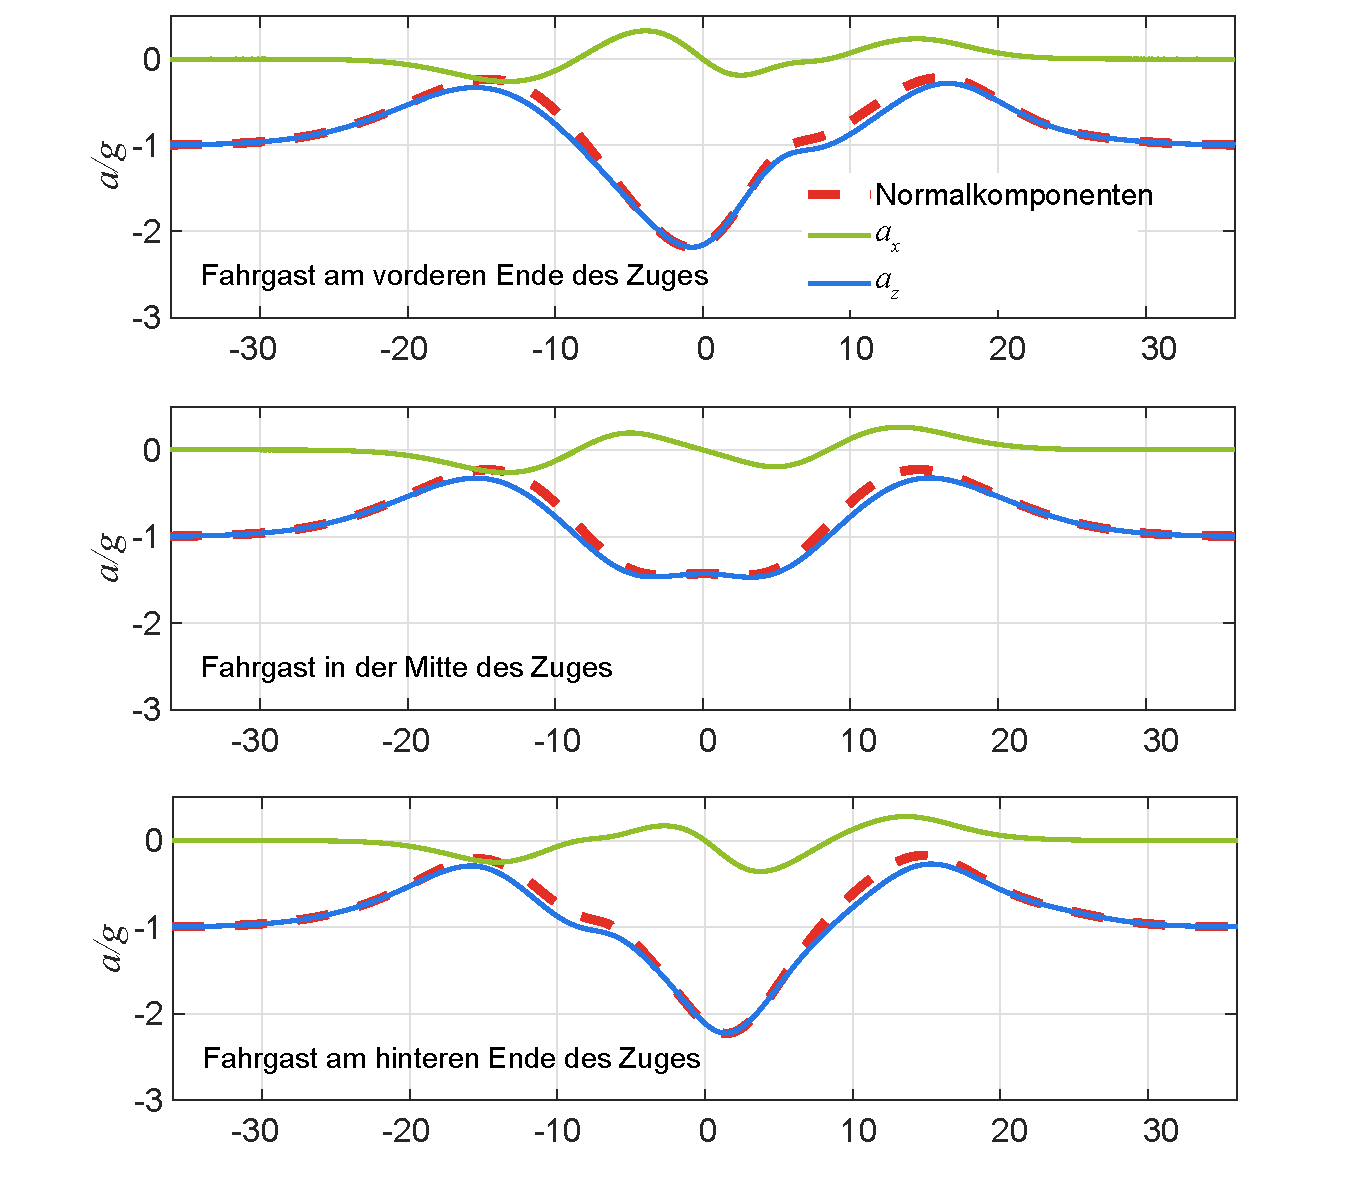
\includegraphics[width=\textwidth]{ABKontNormBeschl.pdf}
  \caption[Normalbeschleunigung auf einen Fahrgast im Achterbahnzug.]{Normalbeschleunigung auf einen Fahrgast im
    Achterbahnzug auf der Gau�kurvenstrecke. Gezeigt sind zus�tzlich die
    $x$- und $z$-Komponenten.}
  \label{abb:kontmech_AchterbahnKontNormalBeschl}
\end{figure}

Ein Beispiel f�r eine L�sung wird im \matlab{}-Programm
\mlkontmechref{AchterbahnKontBeschl.m} vorgestellt.
Die Normalbeschleunigung sowie ihre $x$- und $z$-Komponenten sind in
\figref{kontmech_AchterbahnKontNormalBeschl} f�r den Fall einer
Gau�-Kurve als Achterbahn dargestellt. Im Vergleich mit dem
diskreten Modell, das wir aus der \hyperref[lsg:bew_achterbahn_diskret]{L�sung}
zu \probref{bew_achterbahn_diskret} kennen, f�llt zun�chst auf, dass die
Kr�fte deutlich weniger symmetrisch um den Berg der Achterbahn wirken. Das
liegt daran, dass im elastischen kontinuierlichen Modell deutlich st�rker
Energie in die Schwingungsbewegung eingekoppelt wird, als es bei diskreten
Wagen, die mit wenigen harten Federn verbunden sind, der Fall ist. Dadurch
wirkt die Form der Kraft auch deutlich unruhiger.
Der qualitative Verlauf des diskreten Modells best�tigt sich jedoch. Um
den Berg herum, ist eine deutliche negative (also nach innen bzw. unten
gerichtete) Normalkraft n�tig, um den Fahrgast auf der Bahn zu halten.
W�hrend er sich zwischen Sitz und Sicherheitshaltung bewegt hat der das Gef�hl,
abzuheben (Airtime) und wird dann aus seiner Sicht in die Sicherheitshaltung
gedr�ckt. Ebenfalls wie im diskreten Modell zeigt sich, dass ein Fahrgast im
mittleren Wagen um den Berg herum eine schw�chere Normalkraft erf�hrt als
Fahrg�ste am Rand.

\end{sol} 
\textcolor{blue} {$\rightarrow$ zur} \probref{kontmech_AchterbahnBeschleunigungen}.\\
\noindent\rule[1ex]{\textwidth}{0.5pt}  \newpage  \clearpage

%-----------------------------------------------------------------------------------------------------------

\begin{sol}{prob:kontmech_ElastizitaetTorsion}\label{lsg:kontmech_ElastizitaetTorsion} %�bung21
\textbf{Elastizit�ts-/Torsionsmodul im dreidimensionalen Spannungstensor}\\ \\

Der Spannungstensor eines elastischen, dreidimensionalen K�rpers hat die
Form
\begin{equation}
  \sigma_{ij} = i \lk  \frac{\partial u_i}{\partial p_j} +
  \frac{\partial u_j}{\partial p_i} \rk + \lambda
  \sum_k \frac{\partial u_k}{\partial p_k} \delta_{ij}
  \label{eq:kontmech_SpannungstensorAufg}
\end{equation}
mit
\begin{subequations}
  \begin{align}
    \lambda &= \frac{j}{(1-2j)(1+j)} E \; ,
              \label{eq:kontmech_ElModAufg} \\
    i &= G = \frac{1}{2} \frac{1}{1+j} E \; .
          \label{eq:kontmechTorModAufg}
  \end{align}
\end{subequations}

Aus diesem m�ssen sich Elastizit�ts- und Torsionsmodul erneut gewinnen
lassen.

Ein Fall, in dem sich ausschlie�lich ein Elastizit�tsmodul bemerkbar macht,
entspricht einer Streckung oder Stauchung in Richtung der Kraftwirkung.
Wir ben�tigen also ein Element $\sigma_{ii}$ des Spannungstensors.
Beispielhaft rechnen wir dies f�r das Element $\sigma_{xx}$ durch. Zusammen
mit den Lam\'e-Konstanten \eqref{eq:kontmech_ElModAufg} und
\eqref{eq:kontmechTorModAufg} erhalten wir in der Definition
\eqref{eq:kontmech_SpannungstensorAufg} des Spannungstensors
\begin{multline}
  \sigma_{xx} = 2 i \frac{\partial u_x}{\partial p_x}
  + \lambda \lk \frac{\partial u_x}{\partial p_x} +
  \frac{\partial u_y}{\partial p_y} + \frac{\partial u_z}{\partial p_z} \rk
  = 2 i \frac{\partial u_x}{\partial p_x}
  + \lambda \lk 1-2j \rk \frac{\partial u_x}{\partial p_x} \\
  = 2 \frac{1}{2} \frac{1}{1+j} E \frac{\partial u_x}{\partial p_x}
  + \frac{j}{(1-2j)(1+j)} E \lk 1-2j \rk \frac{\partial u_x}
  {\partial p_x} \\
  = \frac{1 + j}{1+j} E \frac{\partial u_x}{\partial p_x}
  = E \frac{\partial u_x}{\partial p_x}
  = E \frac{\Delta \ell}{\ell}
\end{multline}
Es ergibt sich also genau die Streckung oder Stauchung mit dem
Elastizit�tsmodul.

Eine Scherung entspricht einem tangentialen Angreifen der Kraft, beispielsweise
ist ausschlie�lich die Verschiebung
\begin{equation*}
  \frac{\partial u_y}{\partial p_x}
\end{equation*}
nichtverschwindend, weil die Verschiebung einer Ebene mit konstantem $p_x$ in
Richtung $u_y$ betrachtet wird. Die zugeh�rigen Elemente des Spannungstensors
lauten
\begin{equation}
  \sigma_{xy} = \sigma_{yx} = i \frac{\partial u_y}{\partial p_x}
  = G \frac{\partial u_y}{\partial p_x} \; .
\end{equation}
Daher ist es sehr konsequent, dass das Torsionsmodul direkt im
Spannungstensor als Vorfaktor auftritt.

\end{sol} 
\textcolor{blue} {$\rightarrow$ zur} \probref{kontmech_ElastizitaetTorsion}.\\
\noindent\rule[1ex]{\textwidth}{0.5pt}  \newpage  \clearpage

%-----------------------------------------------------------------------------------------------------------

\begin{sol}{prob:kontmech_BogenSpannung}\label{lsg:kontmech_BogenSpannung} %�bung22
  \textbf{Bogen mit Spannung durch eine Saite}\\ \\

  Um die Schwingungsfrequenz des Bogens zu berechnen, l�sen wir die
  Differentialgleichung
  \begin{equation*}
    \frac{\partial^4 n}{\partial s^2} = 
    \frac{m \omega^2}{E I h} n + \frac{F}{E I h} \; .
  \end{equation*}
  Sie l�sst sich sehr gut mit einem Runge-Kutta-Algorithmus 4. Ordnung
  und fester Schrittweite integrieren. Dazu schreiben wir die
  Differentialgleichung 4. Ordnung in vier Differentialgleichungen 1. Ordnung
  um,
  \begin{align*}
    \frac{\partial n_0}{\partial s} &= n_1 \; , \\
    \frac{\partial n_1}{\partial s} &= n_2 \; , \\
    \frac{\partial n_2}{\partial s} &= n_3 \; , \\
    \frac{\partial n_3}{\partial s} &=
    \frac{m \omega^2}{E I h} n + \frac{F}{E I h} \; .
  \end{align*}
  Als Startwerte f�r die Integration werden $n_0(0) = n_a$, $n_1(0) = n'_a$,
  $n_2(0) = 0$ und $n_3(0) = 0$ verwendet. Die Werte von $n'_a$ und $\omega$
  werden so lange variiert, bis am Ende der Integration bei $s=L$ die
  Randbedingungen $n_2(L) = 0$ und $n_3(L) = 0$ erf�llt sind. Dies
  l�sst sich mit der nichtlinearen Nullstellensuche \texttt{fsolve} aus
  der Optimization Toolbox von \matlab{} automatisiert umsetzen. Ein
  Beispielprogramm ist in der \matlab{}-Datei \mlkontmechref{GespannterBogen.m}
  gegeben.

  Das Beispielprogramm arbeitet mit 2000 Integrationsschritten. Jeweils 10
  Schritte vom Rand wird die Spannkraft der Saite mit
  \begin{equation*}
    F= T_1 \cos(\vartheta)\, \left | \frac{\partial n}{\partial s} \right |
    - 2k\,n\, \sin^2(\vartheta)
  \end{equation*}
  angesetzt. Der Betrag wird eingef�hrt, um sicherzustellen, dass die
  Spannkraft unabh�ngig vom Vorzeichen der gew�hlten Anfangsbedingungen immer
  in dieselbe Richtung zeigt. Die Saite zieht am Bogen. In allen anderen
  Integrationsschritten gilt $F=0$. F�r die Bestimmung der Eigenfrequenz des
  Bogens ohne spannende Saite wird $F=0$ in allen Integrationsschritten
  angesetzt.
  
  F�r die Parameter aus der Aufgabenstellung ist die Schwingungsfrequenz
  ohne Saite ($f_0$) und f�r die Spannkr�fte von $T_1 = \SI{20}{\newton}$,
  $\SI{50}{\newton}$ und $\SI{100}{\newton}$ in
  \figref{kontmech_GespannterBogen1} gezeigt. Man sieht deutlich, dass bei
  niedrigen Biegungen in der Ruhelage (kleinen Winkeln $\vartheta$) die
  Schwingungsfrequenz kleiner als f�r den Bogen ohne �u�ere Spannung ist.
  F�r gr��eres $\vartheta$ steigt die Frequenz jedoch an und erreicht
  schlie�lich deutlich h�here Werte als $f_0$.

  \begin{figure}
    \centering
    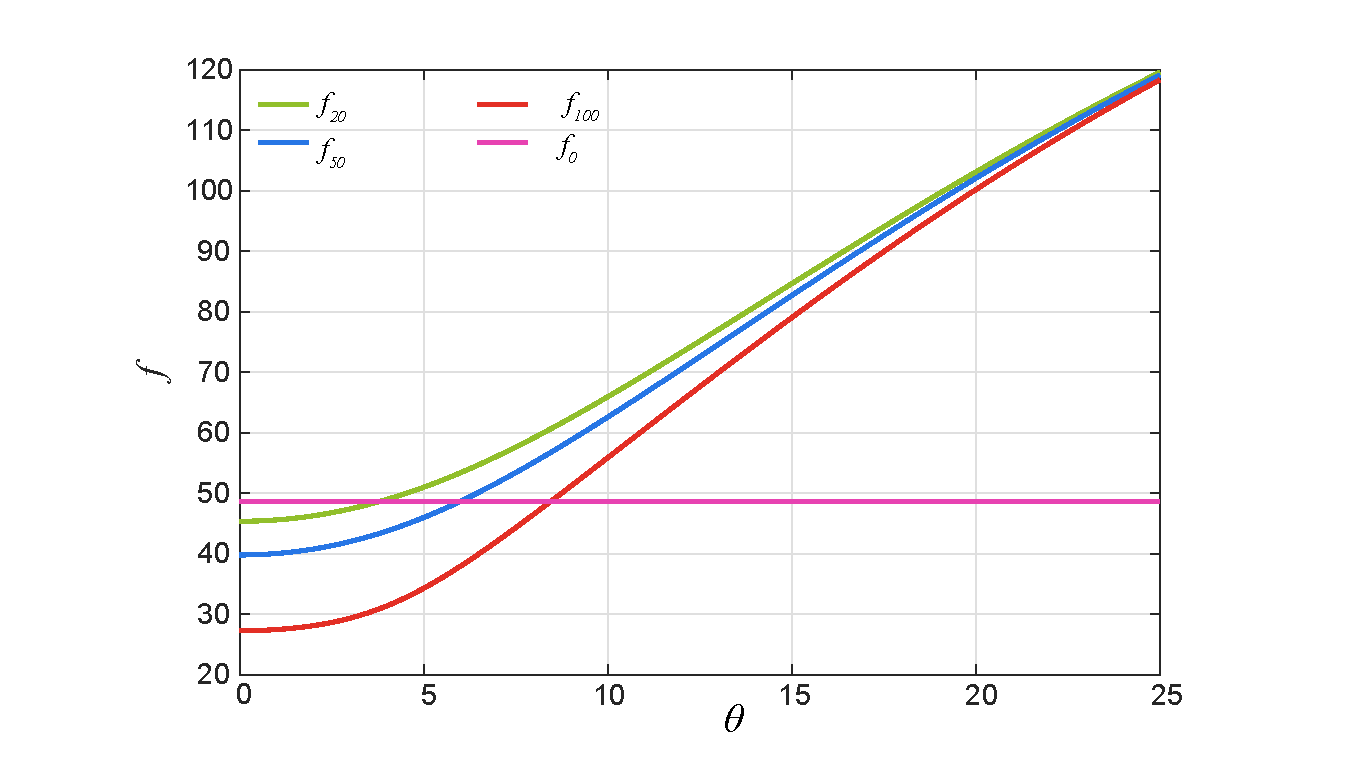
\includegraphics[width=\textwidth]{GespannterBogen1.pdf}
    \caption[Schwingungsfrequenzen eines gespannten Bogens.]
    {Schwingungsfrequenzen eines gespannten Bogens f�r verschiedene
      Winkel $\theta$ der Kr�mmung in der Ruhelage.}
    \label{abb:kontmech_GespannterBogen1}
  \end{figure}

  Der Grund f�r die zwei verschiedenen Verhalten l�sst sich mit den
  verschiedenen Richtungen erkl�ren, in denen die Saite wirkt. F�r einen
  geraden Bogen ($\vartheta = 0$) oder eine schwache Kr�mmung entsteht erst
  durch die Auslenkung der Schwingung eine von der Saite verursachte
  Kraftkomponente senkrecht zur Achse des Bogens, also in Richtung der
  Auslenkung. Diese unterst�tzt die Auslenkung. Der Bogen wirkt dadurch
  weicher und die Schwingungsfrequenz sinkt \cite{Cross2001}. Bei einer
  gr��eren Kr�mmung �berwiegt der Effekt, dass der Bogen durch die Form
  bereits eine Spannkraft hat, die durch die Spannkraft der Saite unterst�tzt
  wird. �hnlich wie in dem Fall, dass parallel an zwei Federn gezogen wird,
  addieren sich die Federkonstanten und der Bogen wird steifer
  \cite{Cross2001}. Die Schwingungsfrequenz steigt folglich.

  Damit l�sst sich auch der Unterschied der Wirkung der gespannten Saite
  auf einen Bogen und einen Schl�ger erkl�ren. Bei einem Schl�ger sind die
  Saiten eintlang der Hauptachsen des Schl�gers gespannt. Sie verursachen
  die Kr�mmung des Schl�gers nicht. Das kommt dem Fall einer sehr geringen
  Kr�mmung $\vartheta \approx 0$ sehr nahe und wie oben beschrieben unterst�tzt
  die Saite damit die Schwingungsbewegung. Sie l�sst den Schl�ger weicher
  wirken. Anders sieht es bei einem Bogen aus. Bei diesem ist die Saite
  typischerweise so gespannt, dass die Kr�mmung des Bogens erst durch sie
  gegeben ist oder die Saite diese verst�rkt. Wir sind also im Fall eines
  gro�en Winkels $\vartheta \gg 0$ und die Saite verst�rkt die R�ckstellkr�ft.
  Sie l�sst den Bogen h�rter wirken als im Fall ohne Saite.
  
  Eine typische Auslenkung und deren erste Ableitung ist f�r den h�chsten
  Winkel $\vartheta = 25^\circ$ im Fall der Federspannung
  $T_1 = \SI{100}{\newton}$ in \figref{kontmech_GespannterBogen2} dargestellt.
  Die zweite und dritte Ableitung sind in \figref{kontmech_GespannterBogen3}
  aufgetragen. Den Einfluss der Seite kann an an den beiden Stellen, an denen
  sie angreift, gut erkennen.

  \begin{figure}
    \centering
    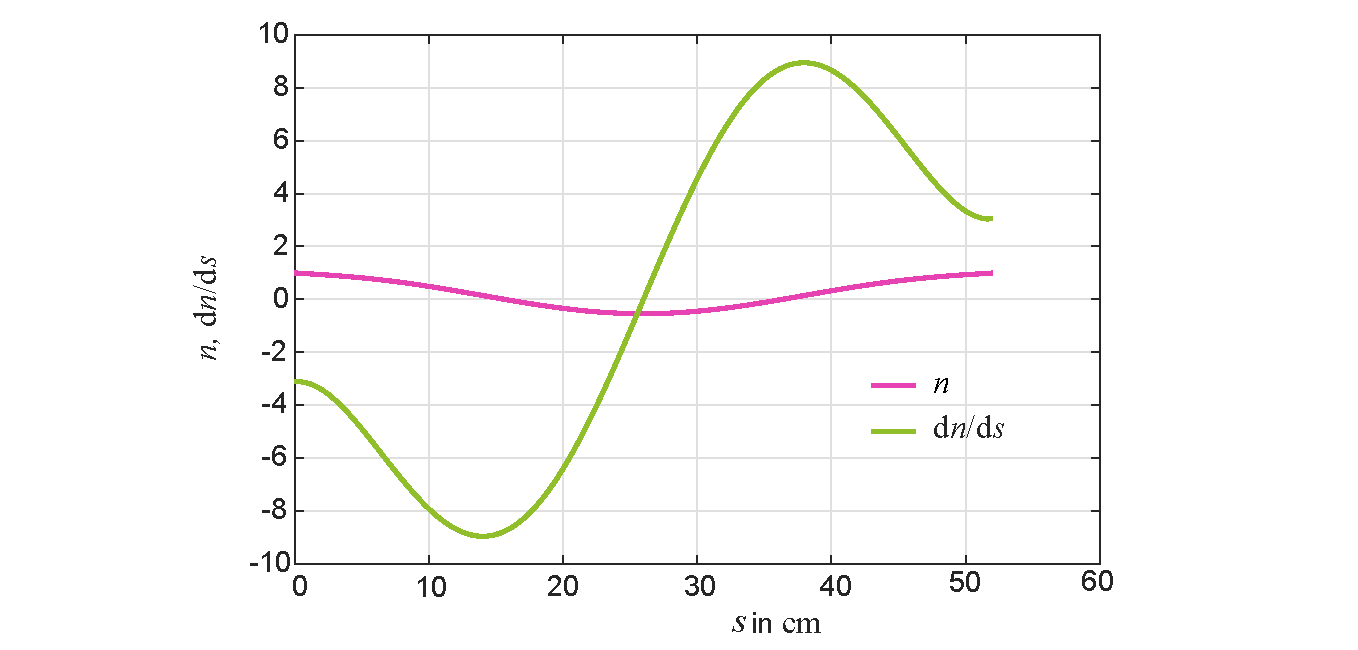
\includegraphics[width=\textwidth]{GespannterBogen2.pdf}
    \caption[Auslenkung der Schwingung eines gespannten Bogens.]
    {Auslenkung der Schwingung eines gespannten Bogens f�r den
      Winkel $\theta = 25^\circ$ und die Spannkraft $T_1 = \SI{100}{\newton}$.}
    \label{abb:kontmech_GespannterBogen2}
  \end{figure}

  \begin{figure}
    \centering
    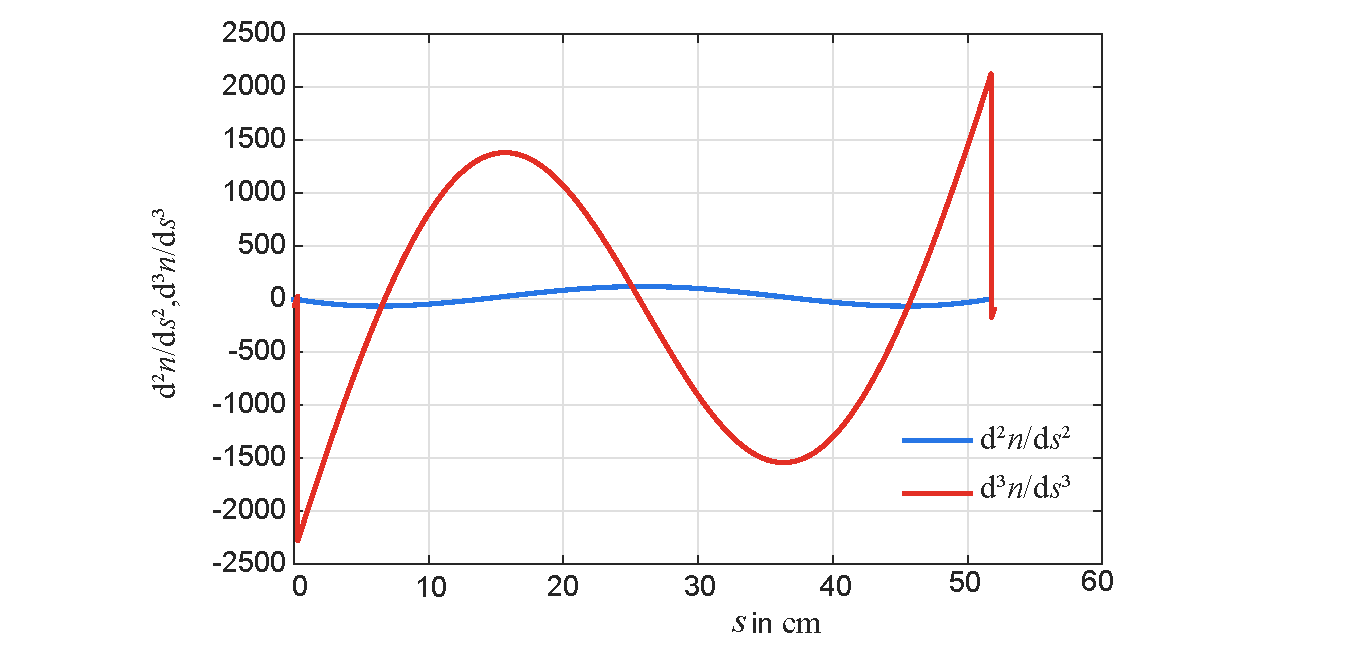
\includegraphics[width=\textwidth]{GespannterBogen3.pdf}
    \caption[Zweite und dritte Ableitung der Schwingung eines gespannten Bogens.]
    {Zweite und dritte Ableitung der Auslenkung der Schwingung eines gespannten
      Bogens f�r den Winkel $\theta = 25^\circ$ und die Spannkraft
      $T_1 = \SI{100}{\newton}$.}
    \label{abb:kontmech_GespannterBogen3}
  \end{figure}
\end{sol} 
\textcolor{blue} {$\rightarrow$ zur} \probref{kontmech_BogenSpannung}.\\
\noindent\rule[1ex]{\textwidth}{0.5pt}  \newpage  \clearpage

%-----------------------------------------------------------------------------------------------------------

\begin{sol}{prob:kontmech_Chladni}\label{lsg:kontmech_Chladni} %�bung23
\textbf{Chladnische Klangfiguren}\\ \\

Die schwingende Scheibe stellt einen zweidimensionalen elastischen K�rper
dar. F�r die Berechnung legen wir die Koordinaten der Scheibe in die
$x$-$y$-Ebene und beschreiben die Auslenkung aus der Ruhelage durch eine
Verschiebung $u_z(x,y,t)$ in $z$-Richtung. Die Differentialgleichung f�r die
elastische Scheibe l�sst sich entsprechend zu
\begin{equation}
  \varrho \frac{\partial^2 z(x,y,t)}{\partial t^2} = i \lk
  \frac{\partial^2 z(x,y,t)}{\partial x^2}
  + \frac{\partial^2 z(x,y,t)}{\partial y^2} \rk
  \label{eq:kontmech_schwingendeScheibe}
\end{equation}
aufstellen. Die Randbedingung bestehen darin, dass auf dem Kreisring, der
die Scheibe begrenzt, die Auslenkung verschwindet, $z=0$.

Ein solches Problem l�sst sich mit der Partial Differential Equation Toolbox
von \matlab{} recht einfach l�sen, indem man die Differentialgleichung
aufstellt und dann mittels des \matlab{}-Kommandos \mlcmd{solvepdeeig}
l�st. Ein Beispiel f�r eine runde Gummischeibe ist in der \matlab{}-Datei
\mlkontmechref{Chladni01.m} gegeben. In \figref{kontmech_ChladniKreis} sind
die L�sungen f�r die ersten sechs Eigenwerte gezeigt.


Vollkommen analog l�sst sich das Problem f�r eine andere Form der Scheibe
l�sen. Einzig die Form des Rands �ndert sich und die Randbedingungen m�ssen
daran angepasst werden. In Abbildung \figref{kontmech_ChladniQuadrat}
ist dies f�r eine quadratische Platte gezeigt, die wiederum nur ein
Spezialfall der rechteckigen Platte aus \figref{kontmech_ChladniRechteck}
ist. Die zugeh�rigen \matlab{}-Dateien sind \mlkontmechref{Chladni02.m}
und \mlkontmechref{Chladni03.m}.

\newpage
\begin{figure}
  \centering
  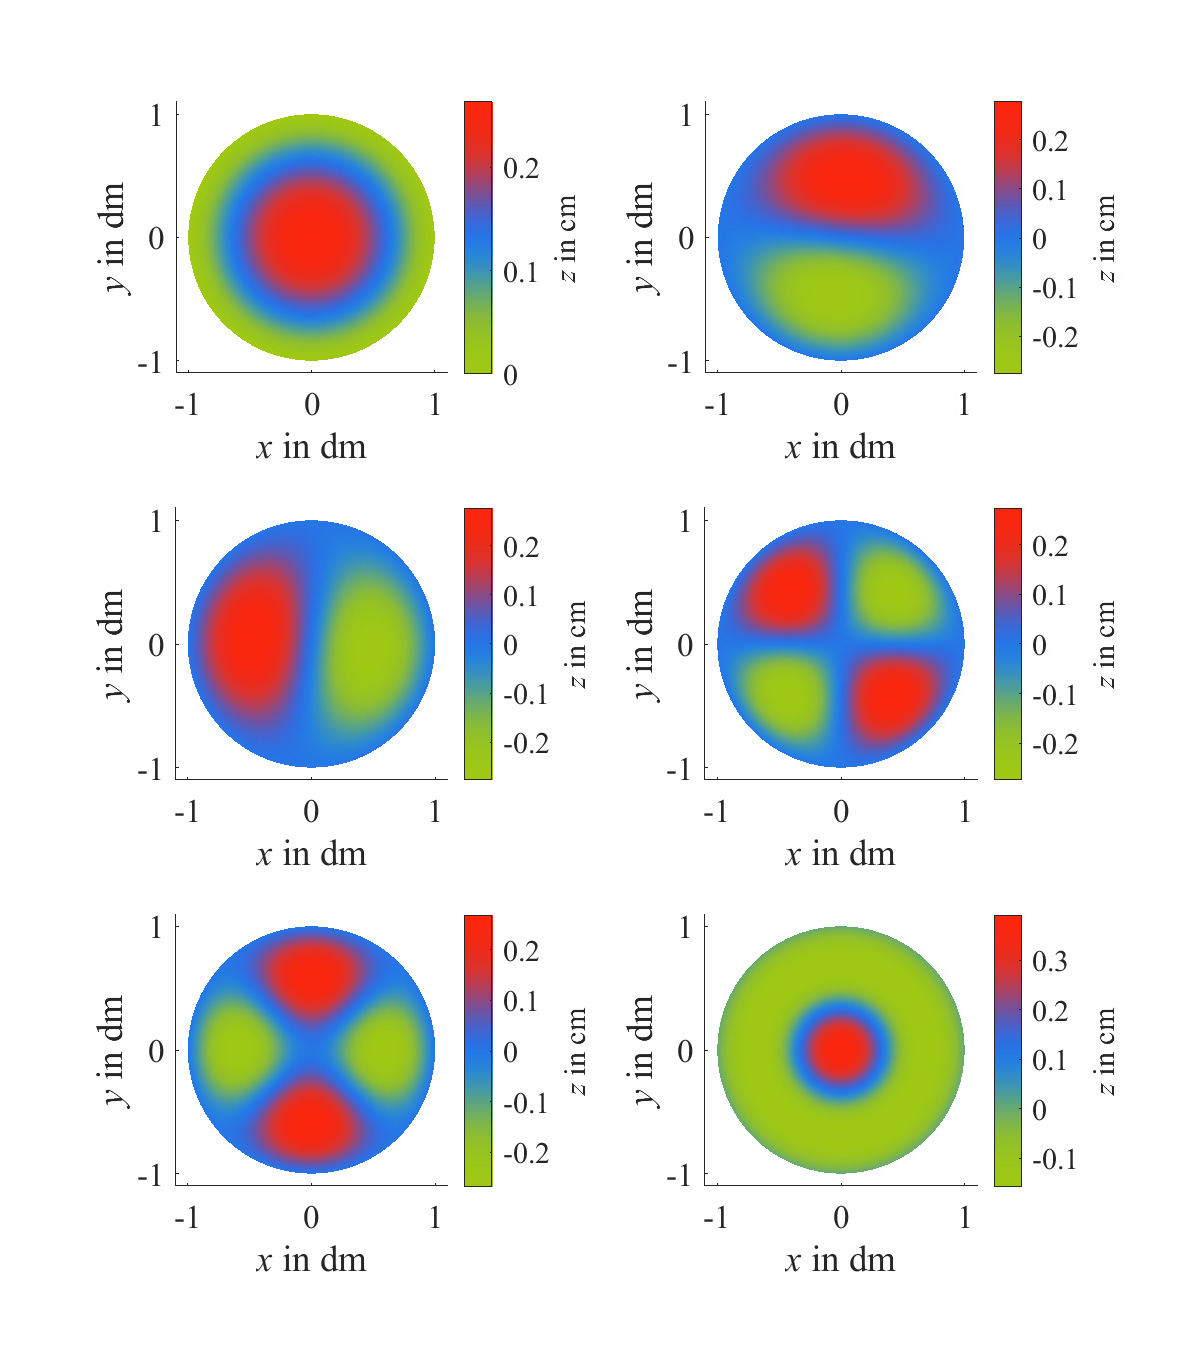
\includegraphics[width=\textwidth]{Chladni_Kreis.pdf}
  \caption[Chladnische Klangfiguren f�r eine kreisf�rmige Fl�che.]
  {Chladnische Klangfiguren f�r eine kreisf�rmige Fl�che. Dargestellt sind die
    numerischen L�sungen f�r die ersten sechs Eigenschwingungen der
    elastischen Fl�che.}
  \label{abb:kontmech_ChladniKreis}
\end{figure}

\newpage
\begin{figure}
  \centering
  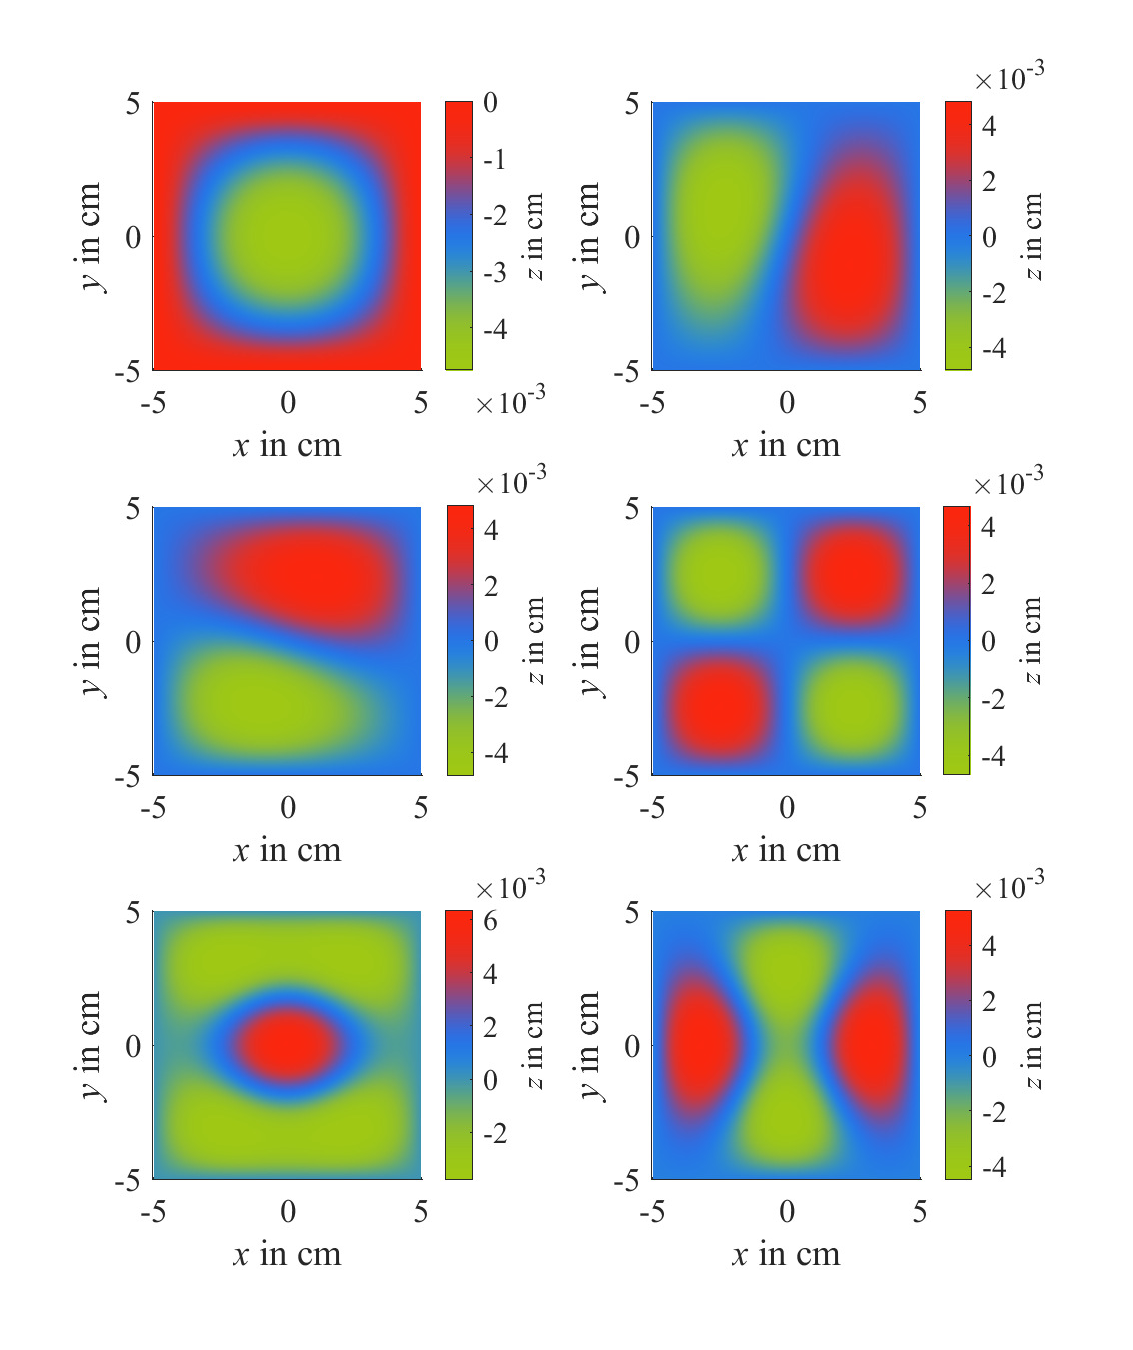
\includegraphics[width=\textwidth]{Chladni_Quadrat.pdf}
  \caption[Chladnische Klangfiguren f�r eine quadratische Fl�che.]
  {Chladnische Klangfiguren f�r eine quadratische Fl�che. Dargestellt sind die
    numerischen L�sungen f�r die ersten sechs Eigenschwingungen der
    elastischen Fl�che.}
  \label{abb:kontmech_ChladniQuadrat}
\end{figure}

\newpage
\begin{figure}
  \centering
  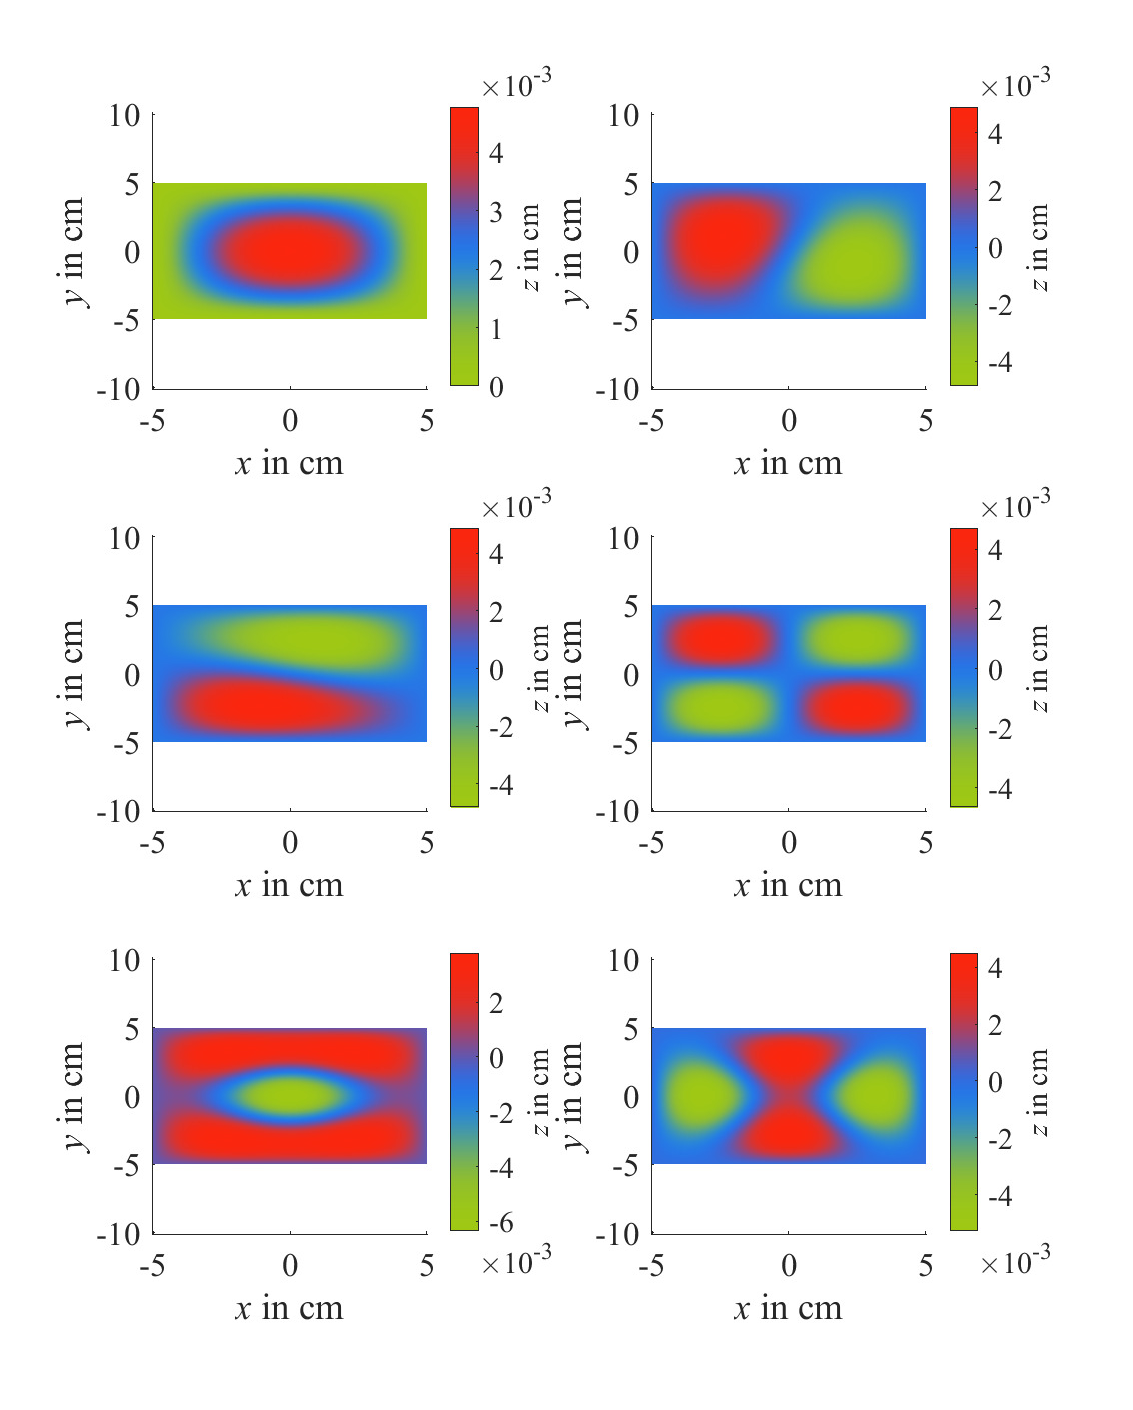
\includegraphics[width=\textwidth]{Chladni_Rechteck.pdf}
  \caption[Chladnische Klangfiguren f�r eine rechteckige Fl�che.]
  {Chladnische Klangfiguren f�r eine rechteckige Fl�che. Dargestellt sind die
    numerischen L�sungen f�r die ersten sechs Eigenschwingungen der
    elastischen Fl�che.}
  \label{abb:kontmech_ChladniRechteck}
\end{figure}

\end{sol} 
\textcolor{blue} {$\rightarrow$ zur} \probref{kontmech_Chladni}.\\
\noindent\rule[1ex]{\textwidth}{0.5pt}  \newpage  \clearpage

% ----------------------------------------------------------------------------------------------------------
% ----------------------------------------------------------------------------------------------------------

\newpage
\subsection{�bungen zu Wellen}

\medskip

% ----------------------------------------------------------------------------------------------------------

%-----------------------------------------------------------------------------------------------------------

\begin{sol}{prob:kontmech_Dispersion}\label{lsg:kontmech_Dispersion} %�bung24
\textbf{Wellenausbreitung und Dispersion}\\

Die L�sung ist im Detail im \mscr{} \mlkontmechref{DispersionWelle.m} hinterlegt.
  \begin{figure}
    \centering
    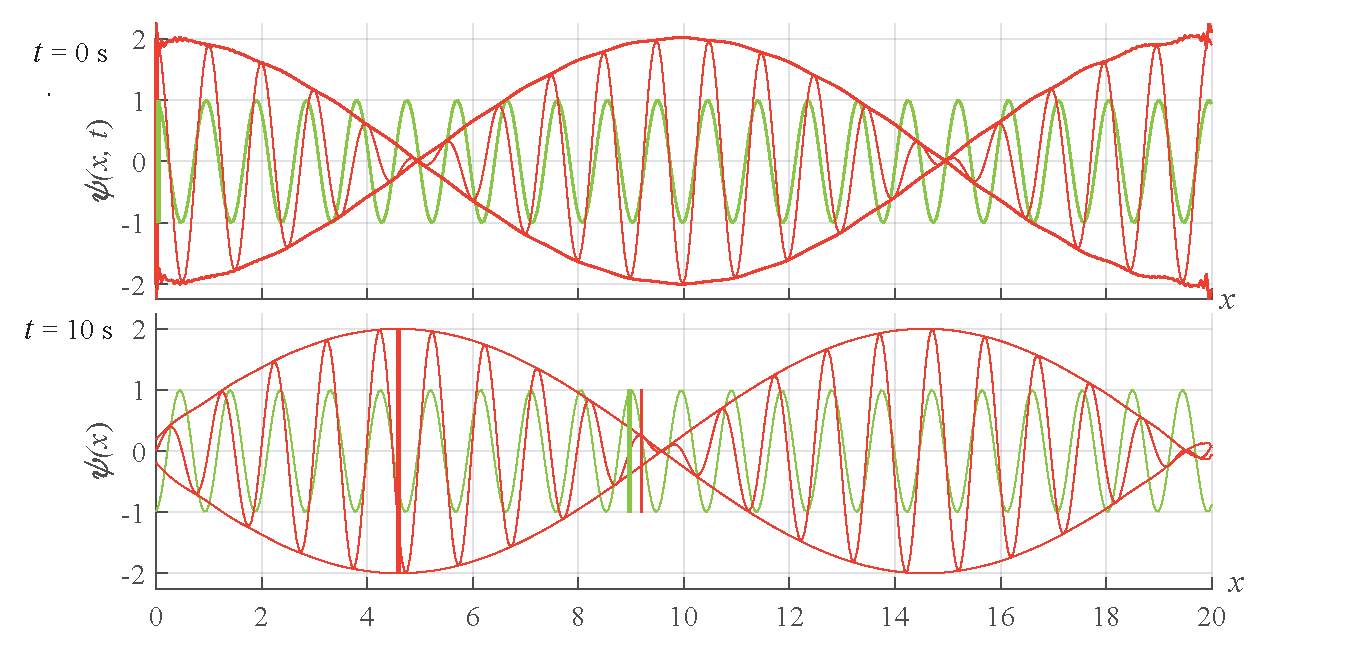
\includegraphics[width=0.85\textwidth]{DispersionWelle.pdf}
    \caption[Ausbreitung einer �berlagerung von zwei Wellen �hnlicher Wellenl�nge.]
    {Ausbreitung einer �berlagerung von zwei Wellen �hnlicher Wellenl�nge. Die Wellenfunktion ist zu zwei verschiedenen Zeitpunkten gezeigt. Deutlich sind die Unterschiede von Phasen- und Gruppengeschwindigkeit erkennbar, der blaue Balken zeigt die Fortbewegung der Einh�llenden und der gr�ne Balken die der Phase. Bei den gew�hlten Parametern liegt normale Dispersion vor mit $v_\text{gr} = 0.5\, v_\text{ph}$.}
    \label{abb:kontmech_Dispersion01}
  \end{figure}
  \begin{figure}
    \centering
    \includegraphics[width=0.85\textwidth]{DispersionWellenPaket.pdf}
    \caption[Ausbreitung eines Wellenpakets.]
    {Ausbreitung eines Wellenpakets aus der �berlagerung von 50 einzelnen Wellen.}
    \label{abb:kontmech_Dispersion02}
  \end{figure}

\end{sol} 
\textcolor{blue} {$\rightarrow$ zur} \probref{kontmech_Dispersion}.\\
\noindent\rule[1ex]{\textwidth}{0.5pt}  \newpage  \clearpage

%-----------------------------------------------------------------------------------------------------------

\begin{sol}{prob:kontmech_Dispersion2}\label{lsg:kontmech_Dispersion2} %�bung25
\textbf{Ausbreitung eines Wellenpakets unter Dispersion}\\ \\

Die L�sung ist im Detail im \mscr{} \mlkontmechref{DispersionWellenpaket.m} hinterlegt.
Im einzelnen erfolgte die L�sung in folgenden Schritten:

\begin{enumerate}
\item Man berechne den Anfangsimpuls $\psi(x_n,t=0)$ im Ortsraum $0 \leq x_n \leq x_\text{end} =  \SI{4000}{\metre}, N_x = 40000,\,\delta x = \SI{0.1}{\metre}$. Aufgrund der zeitlichen Ausdehnung hat der Anfangsimpuls auch eine r�umliche Ausdehnung.
\item Man transformiere den Anfangsimpuls in den Fourier-Raum und erh�lt: $\Psi(k,t=0)$ F�r die Raumfrequenz bzw. Wellenzahl gilt: $0 \leq k_n \leq k_\text{end} = 2\pi / \delta x = 2\pi \SI{10}{\metre},\, N_k = 40000$.
\item Man bestimme die Phasengeschwindigkeiten $v_{\text{Ph},n}(k_n)$ und die Kreisfrequenzen $\omega_n(k_n)$ als Funktion der Wellenzahlen Dabei benutze man die gegebene Dispersionsrelation $v_ph(k)$.
\item Die Ausbreitung durch das Medium wird als zeitliche Evolution im Frequenzraum mit der Filterfunktion $\mathrm{exp}(\im \omega_n\,t_\text{mess})$ beschrieben, worin $t_\text{mess}$ die Zeit der Propagation durch das Medium ist.
\item Man multipliziere $\mathrm{exp}(\im \omega_n\,t_\text{mess})$ mit $\Psi(k_n,t=0)$ und bilde die R�cktransformation, was schlie�lich $\psi(x_n, t=t_\text{mess})$ ergibt.
\item Man erkennt sehr sch�n, dass sich das Wellenpaket bei der Ausbreitung im dispersiven Medium verbreitert (Energie bleibt konstant aber Intensit�t verringert sich) und als ganzes mit der Gruppengeschwindigkeit vorw�rts bewegt.
\end{enumerate}

  \begin{figure}
    \centering
    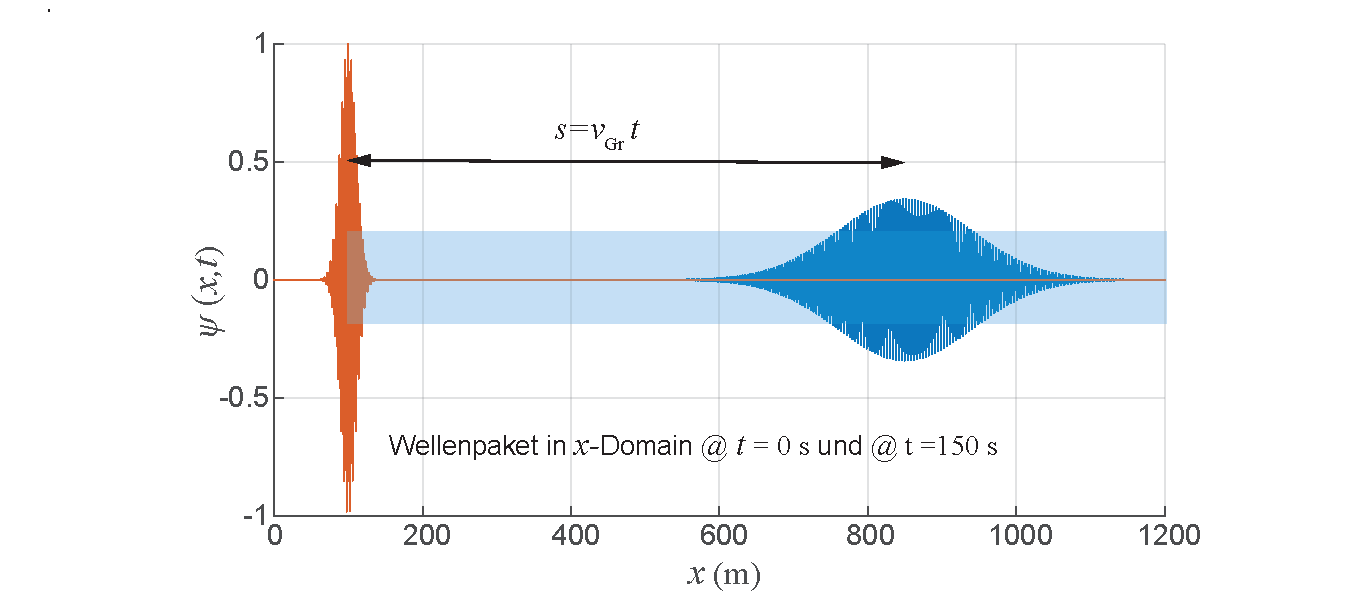
\includegraphics[width=\textwidth]{DispersionGaussWellenpaket.pdf}
    \caption[Ausbreitung eines Gau�-Wellenpakets in einem dispersivem Medium.]
    {Ausbreitung eines Gau�-Wellenpakets in einem dispersivem Medium. Man erkennt deutlich die Verbreiterung (das Auseinanderflie�en) des Wellenpakets, das sich selbst mit der Gruppengeschwindigkeit $v_\text{Gr}$ im Medium ausbreitet.}
    \label{abb:kontmech_DispersionGauss01}
  \end{figure}

Hinweise:
\begin{itemize}
	\item Die dargestellte Berechnung kann auch erfolgen, indem man von einer zeitlichen Anfangsverteilung ausgeht und dann im Fourier-Raum die Propagation durch das Medium betrachtet. Der entsprechende Propagator enth�lt dann die L�nge des Mediums als Messgr��e (Zusatz�bung).
	\item Wie erw�hnt liegt die Grundlage der beschriebenen Vorgehensweise in der Linearit�t der Wellengleichung. F�r den Gau�-f�rmigen Impuls kann man die L�sung auch analytisch berechnen (Zusatz�bung). Wir werden das im Band Optik an Hand der Wellengleichung f�r Lichtimpulse behandeln.
	\item Laut Vorgabe haben wir eine lineare Abh�ngigkeit der Phasengeschwindigkeit von der Wellenzahl, die Gruppengeschwindigkeit ist somit eine Konstante und zeigt selbst keine Dispersion. Im Allgemeinen zeigt auch die Gruppengeschwindigkeit eine Dispersion, n�mlich dann, wenn 
		\begin{align*}
			\frac{\d v_\text{Gr}}{\d k} = \frac{\d^2 \omega}{\d k^2} \neq 0\,.
		\end{align*}
	Man hat dann sogenannte Gruppengeschwindigkeitsdispersion vorliegen, die besonders bei optischen Impulsen in Fasern relevant zu ber�cksichtigen ist. Wir werden uns auch damit im Band Optik besch�ftigen.
\end{itemize}


  \begin{figure}
    \centering
    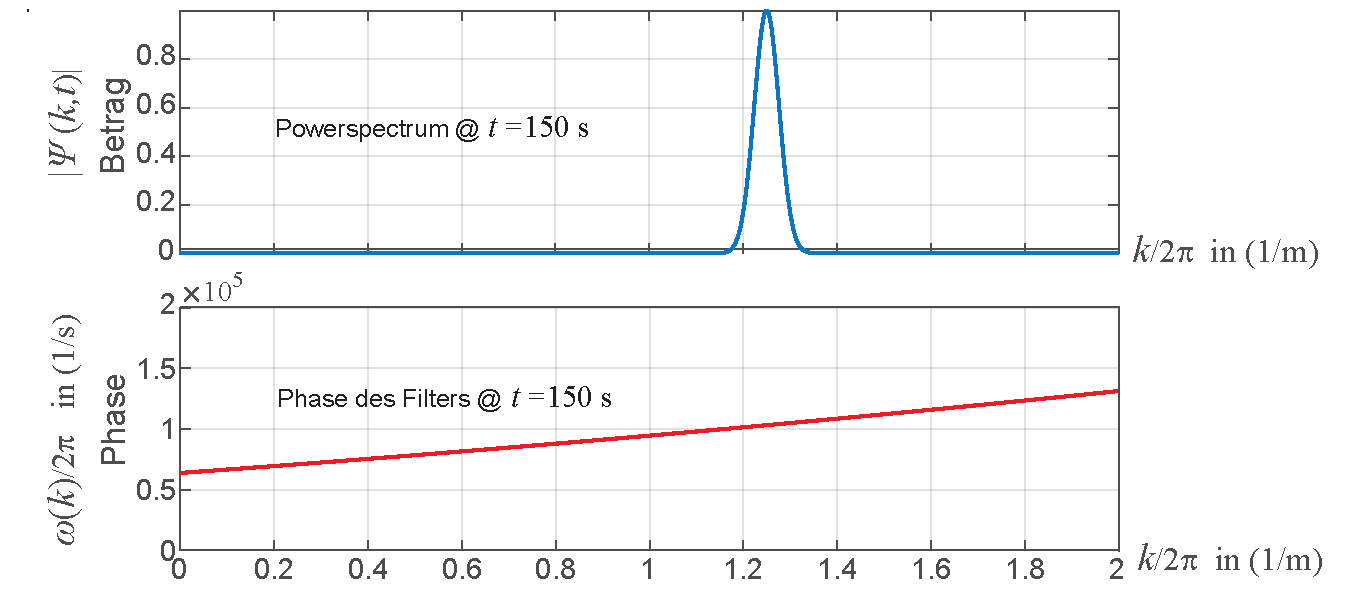
\includegraphics[width=\textwidth]{DispersionGaussWellenpaket02.pdf}
    \caption[Leistungsspektrum eines Gau�-Wellenpakets und Filtercharakteristik eines dispersiven Mediums.]
    {Leistungsspektrum eines Gau�-Wellenpakets und Filtercharakteristik eines dispersiven Mediums.}
    \label{abb:kontmech_DispersionGauss02}
  \end{figure}



\end{sol} 
\textcolor{blue} {$\rightarrow$ zur} \probref{kontmech_Dispersion2}.\\
\noindent\rule[1ex]{\textwidth}{0.5pt}  \newpage  \clearpage

%-----------------------------------------------------------------------------------------------------------

\begin{sol}{prob:kontmech_soliton1}\label{lsg:kontmech_soliton1} %�bung26
\textbf{Solitonen I}\index{Solitonen}\\ \\

Einerseits ist f�r die Korteweg-de-Vries-Gleichung
\begin{equation}
  \frac{\partial \psi}{\partial t} + 6\,\psi\,\frac{\partial \psi}{\partial x}
  + \frac{\partial^3 \psi}{\partial x^3} = 0
  \tag{\ref{eq:kontmech_soliton01}}
\end{equation}
mit
\begin{align}
    \psi(x,t) = \frac{c}{2}\;\sech^2\lek \frac{\sqrt{c}}{2}\;\lk x-ct \rk \rek
  \tag{\ref{eq:kontmech_soliton02}}
\end{align}
eine Einzel-Soliton-L�sung\footnote{Dar�ber hinaus gibt es weitere analytische
  L�sungen, z.B. f�r $N$ Solitonen, die jedoch �ber unsere Betrachtung
  hinausgehen.} analytisch bekannt, andererseits haben wir mit den numerischen
Methoden, partielle Differentialgleichungen zu l�sen, eine M�glichkeit an der
Hand, diese L�sungen genauer zu untersuchen und F�lle zu konstrieren, die
dar�ber hinausgehen. Dies alles wollen wir in dieser L�sung tun.

\begin{enumerate}
\item Zun�chst stellen wir die Soliton-L�sungen \eqref{eq:kontmech_soliton02} 
  dar. Ein Beispiel mit dem Parameter $c=1$ ist in
  \figref{kontmech_KdV1Soliton} gegeben. Eine solche L�sung ver�ndert,
  wie es von einem Soliton zu erwarten ist, ihre Form nicht. Die L�sung
  wandert in der Zeit zu gr��eren Orten $x$, was die einzige erkennbare
  Zeitwenticklung darstellt.

  \begin{figure}
    \centering
    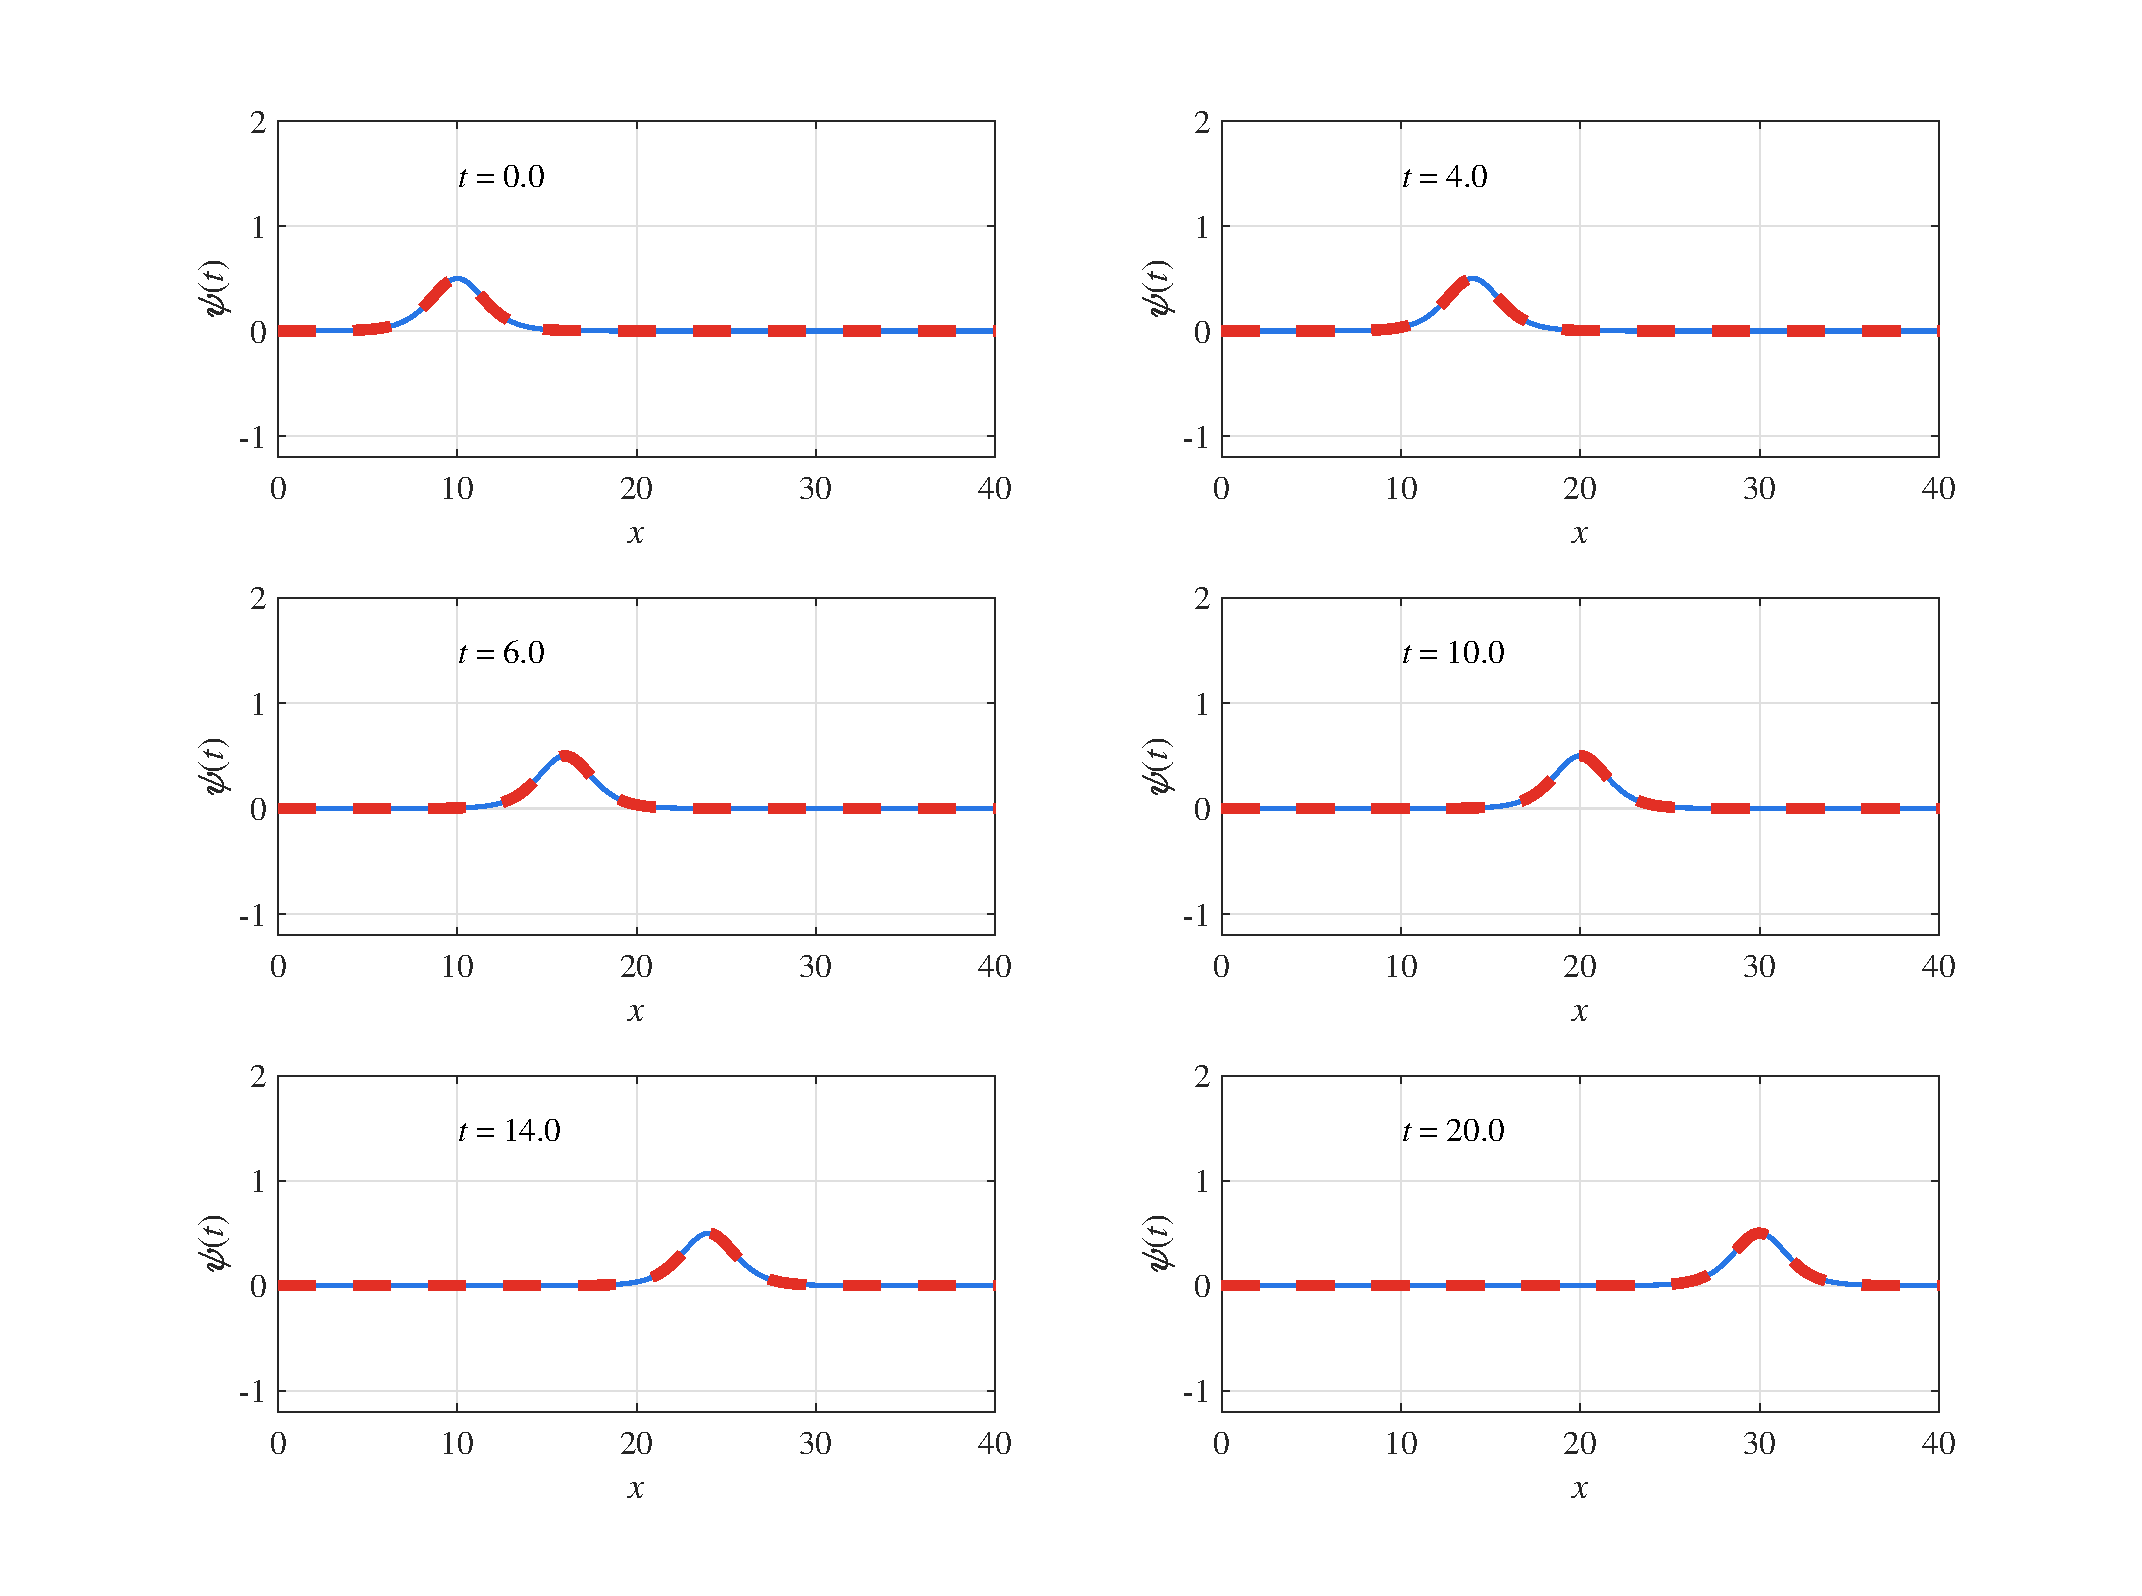
\includegraphics[width=\textwidth]{KdV1Soliton.pdf}
    \caption[Ausbreitung einer Soliton-L�sung der Korteweg-de-Vries-Gleichung.]
    {Ausbreitung einer einzelnen Soliton-L�sung der Korteweg-de-Vries-Gleichung
      nach Gleichung \eqref{eq:kontmech_soliton02} f�r $c = 1$ (blaue,
      durchgezogene Linie). Die Stabilit�t der Form ist erkennbar, w�hrend
      sich das Soliton nach rechts bewegt. Eine numerische L�sung der
      partiellen Differentialgleichung \eqref{eq:kontmech_soliton01} f�hrt f�r
      dieselben Startwerte zum selben Ergebnis (rot gestrichelte Linie).}
    \label{abb:kontmech_KdV1Soliton}
  \end{figure}
  
  Verschiedene L�sungen f�r die Parameter $c = 0.5, 1, 2, 3$ werden in
  \figref{kontmech_KdVSolitonVergleichc} miteinander verglichen. Als erstes
  f�llt auf, dass alle dieselbe grundlegende Form haben. Dies �berrascht nicht
  weiter, da sie alle der Form \eqref{eq:kontmech_soliton02} entsprechen.
  Genauso kann man aus der Gleichung ablesen, dass ein gr��erer Wert von $c$
  zu einem h�heren Maximum von $ \psi$ f�hrt, die Funktion daf�r um das Maximum
  herum schneller abf�llt. Dies findet sich alles in der Darstellung wieder.
  Dar�ber hinaus erkennt man die Stabilit�t der Form f�r alle Werte von
  $c$. Da $c$ die Bedeutung einer Geschwindigkeit hat, breiten die verschiedenen
  L�sungen sich unterschiedlich schnell nach rechts aus. 

  \begin{figure}
    \centering
    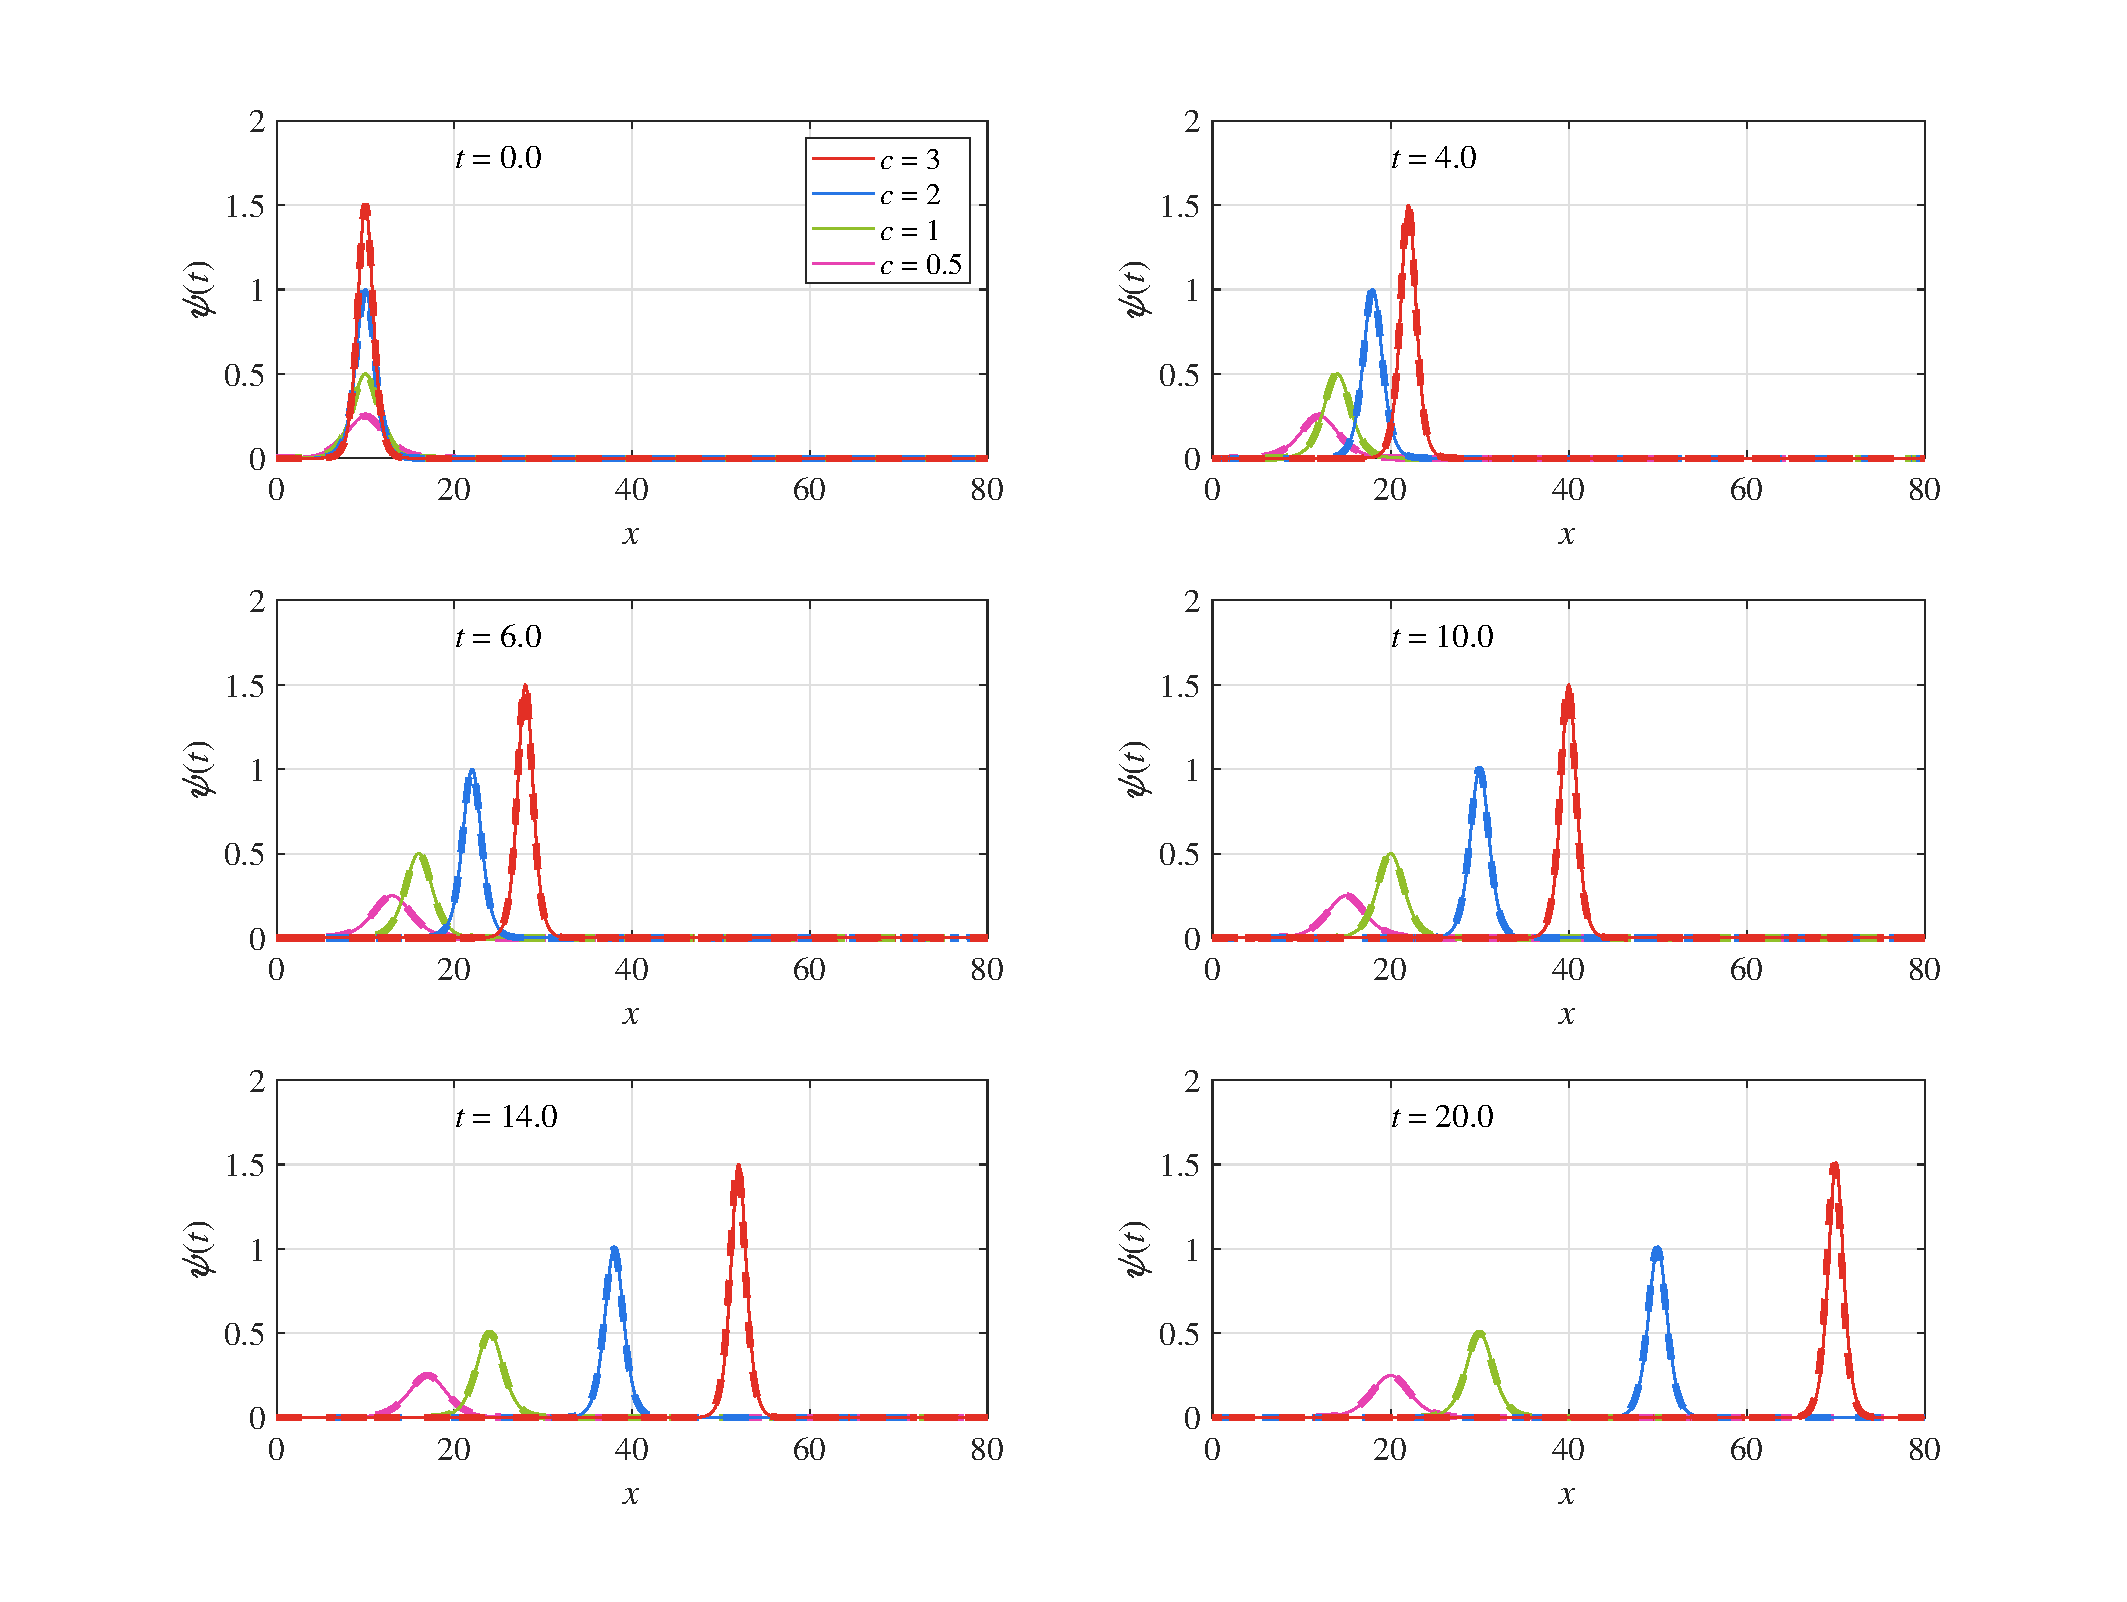
\includegraphics[width=\textwidth]{KdVSolitonVergleichc.pdf}
    \caption[Ausbreitung von Soliton-L�sung der Korteweg-de-Vries-Gleichung mit
    verschiedenem $c$.]
    {Ausbreitung mehrerer Soliton-L�sungen der Korteweg-de-Vries-Gleichung f�r
      die Geschwindigkeitsparamter $c = 0.5, 1, 2, 3$. Bei einer anderen
      Geschwindigkeit muss die L�sung der nichtlinearen Wellengleichung auch
      eine andere Gestalt annehmen, die jedoch derselben grundlegenden Form
      \eqref{eq:kontmech_soliton02} entspricht. Jede L�sung bleibt f�r sich
      stabil. Durchgezogene, d�nne Linien repr�sentieren die analytische
      L�sung \eqref{eq:kontmech_soliton02}, w�hrend gestrichelte, dicke Linien
      die zugh�rige numerische L�sung der partiellen Differentialgleichung
      \eqref{eq:kontmech_soliton01} darstellen.}
    \label{abb:kontmech_KdVSolitonVergleichc}
\end{figure}

\item Wir wollen nun zeigen, dass die Funktion \eqref{eq:kontmech_soliton02}
  tats�chlich eine L�sung der Korteweg-de-Vries-Gleichung
  \eqref{eq:kontmech_soliton01} ist. Dazu schreiben wir die L�sung
  zun�chst als 
  \begin{align}
    \psi(x,t) = \frac{c}{2}\;\sech^2\lek \frac{\sqrt{c}}{2}\;\lk x-ct \rk \rek
    = \frac{c}{2} \frac{1}{\cosh^2\lek \frac{\sqrt{c}}{2}\;\lk x-ct \rk \rek}
  \end{align}
  und bilden die Ableitungen, die wir f�r die weitere Rechnung ben�tigen:
  \begin{subequations}
    \allowdisplaybreaks
    \begin{align}
      \frac{\partial \psi(x,t)}{\partial t}
      &= \frac{c^{5/2}}{2} \frac{\sinh\lek \frac{\sqrt{c}}{2}\;\lk x-ct \rk
        \rek}{\cosh^3\lek \frac{\sqrt{c}}{2}\;\lk x-ct \rk \rek} \; ,\\
      \frac{\partial \psi(x,t)}{\partial x}
      &= -\frac{c^{3/2}}{2} \frac{\sinh\lek \frac{\sqrt{c}}{2}\;\lk x-ct \rk
        \rek}{\cosh^3\lek \frac{\sqrt{c}}{2}\;\lk x-ct \rk \rek} \; ,\\
      \frac{\partial^2 \psi(x,t)}{\partial x^2}
      &= \frac{c^{2}}{4} \left \{ -\frac{1}{\cosh^2\lek \frac{\sqrt{c}}{2}\;
        \lk x-ct \rk \rek} 
        +3 \frac{\sinh^2\lek \frac{\sqrt{c}}{2}\;\lk x-ct \rk
        \rek}{\cosh^4\lek \frac{\sqrt{c}}{2}\;\lk x-ct \rk \rek} \right \} \; ,
      \\
      \frac{\partial^3 \psi(x,t)}{\partial x^3}
      &= \frac{c^{5/2}}{8} \left \{ 8\frac{\sinh\lek \frac{\sqrt{c}}{2}\;
        \lk x-ct \rk \rek}{\cosh^3\lek \frac{\sqrt{c}}{2}\;\lk x-ct \rk \rek} 
       -12 \frac{\sinh^3\lek \frac{\sqrt{c}}{2}\;\lk x-ct \rk
        \rek}{\cosh^5\lek \frac{\sqrt{c}}{2}\;\lk x-ct \rk \rek} \right \}
        \; .
    \end{align}
  \end{subequations}
  Setzt man diese Ableitungen in die Korteweg-de-Vries-Gleichung ein, so
  erh�lt man
  \begin{multline*}
    \frac{c^{5/2}}{2} \frac{\sinh\lek \frac{\sqrt{c}}{2}\;\lk x-ct \rk
      \rek}{\cosh^3\lek \frac{\sqrt{c}}{2}\;\lk x-ct \rk \rek}
    - 6 \; \frac{c}{2} \frac{1}{\cosh^2\lek \frac{\sqrt{c}}{2}\;\lk x-ct \rk
      \rek} \cdot \frac{c^{3/2}}{2} \frac{\sinh\lek \frac{\sqrt{c}}{2}\;
      \lk x-ct \rk \rek}{\cosh^3\lek \frac{\sqrt{c}}{2}\;\lk x-ct \rk \rek}
    \\
    + \frac{c^{5/2}}{8} \left \{ 8\frac{\sinh\lek \frac{\sqrt{c}}{2}\;
        \lk x-ct \rk \rek}{\cosh^3\lek \frac{\sqrt{c}}{2}\;\lk x-ct \rk \rek} 
      -12 \frac{\sinh^3\lek \frac{\sqrt{c}}{2}\;\lk x-ct \rk
        \rek}{\cosh^5\lek \frac{\sqrt{c}}{2}\;\lk x-ct \rk \rek} \right \}
    = 0 \; .
  \end{multline*}
  Um diese Terme besser vergleichen zu k�nnen, multiplizieren wir alle
  mit $4/c^{5/2}$ und bringen sie auf den Hauptnenner
  $\cosh^5\lek \frac{\sqrt{c}}{2}\;\lk x-ct \rk \rek$,
  \begin{multline*}
    2\; \frac{\sinh\lek \frac{\sqrt{c}}{2}\;\lk x-ct \rk \rek \;
      \cosh^2\lek \frac{\sqrt{c}}{2}\;\lk x-ct \rk \rek}
    {\cosh^5\lek \frac{\sqrt{c}}{2}\;\lk x-ct \rk \rek}
    - 6 \; \frac{\sinh\lek \frac{\sqrt{c}}{2}\;\lk x-ct \rk \rek}
    {\cosh^5\lek \frac{\sqrt{c}}{2}\;\lk x-ct \rk \rek} \\
    + 4 \frac{\sinh\lek \frac{\sqrt{c}}{2}\;\lk x-ct \rk \rek \;
      \cosh^2\lek \frac{\sqrt{c}}{2}\;\lk x-ct \rk \rek}
    {\cosh^5\lek \frac{\sqrt{c}}{2}\;\lk x-ct \rk \rek} 
    -6 \frac{\sinh^3\lek \frac{\sqrt{c}}{2}\;\lk x-ct \rk
        \rek}{\cosh^5\lek \frac{\sqrt{c}}{2}\;\lk x-ct \rk \rek} 
    = 0 \; .
  \end{multline*}
  Die linke Seite l�sst sich zusammenfassen zu
  \begin{multline*}
    \frac{6\; \sinh\lek \frac{\sqrt{c}}{2}\;\lk x-ct \rk \rek \left \{
          \cosh^2\lek \frac{\sqrt{c}}{2}\;\lk x-ct \rk \rek
          - \sinh^2\lek \frac{\sqrt{c}}{2}\;\lk x-ct \rk \rek \right \} }
    {\cosh^5\lek \frac{\sqrt{c}}{2}\;\lk x-ct \rk \rek}
    - 6 \; \frac{\sinh\lek \frac{\sqrt{c}}{2}\;\lk x-ct \rk \rek}
    {\cosh^5\lek \frac{\sqrt{c}}{2}\;\lk x-ct \rk \rek} \\
    = \frac{6\; \sinh\lek \frac{\sqrt{c}}{2}\;\lk x-ct \rk \rek}
    {\cosh^5\lek \frac{\sqrt{c}}{2}\;\lk x-ct \rk \rek}
    - 6 \; \frac{\sinh\lek \frac{\sqrt{c}}{2}\;\lk x-ct \rk \rek}
    {\cosh^5\lek \frac{\sqrt{c}}{2}\;\lk x-ct \rk \rek} 
    = 0 \; ,
  \end{multline*}
  und erf�llt somit die rechte Seite. Damit ist gezeigt, dass die Funktion
  \eqref{eq:kontmech_soliton02} eine L�sung der Korteweg-de-Vries-Gleichung
  \eqref{eq:kontmech_soliton01} darstellt.
  
\item Wir wollen nun noch zeigen, dass die Summe $\psi_1+\psi_2$ von zwei
  L�sungen $\psi_1$ und $\psi_2$ der KdV-Gleichung \iA selbst keine
  L�sung darstellt. Dies ist eine Eigenschaft nichtlinearer
  Differentialgleichungen.

  Wir setzen zun�chst die Summe in die KdV-Gleichung ein und erhalten
  \begin{align*}
    \frac{\partial}{\partial t} \lk \psi_1 + \psi_2 \rk
    + 6\,\lk\psi_1 + \psi_2 \rk\,\frac{\partial }{\partial x} \lk \psi_1
    + \psi_2 \rk   
    + \frac{\partial^3}{\partial x^3} \lk \psi_1 + \psi_2 \rk &= 0 \\
    \intertext{bzw.}
    \frac{\partial \psi_1}{\partial t} + \frac{\partial \psi_2}{\partial t}
    + 6\,\lk\psi_1 + \psi_2 \rk\, \lk \frac{\partial \psi_1}{\partial x}
     + \frac{\partial \psi_2}{\partial x} \rk
    + \frac{\partial^3 \psi_1}{\partial x^3}
    + \frac{\partial^3 \psi_2}{\partial x^3} &= 0 \; .
  \end{align*}
  Diese Terme sortieren wir neu zu
  \begin{equation}
    \left \{ \frac{\partial \psi_1}{\partial t} + 6 \, \psi_1 \,
      \frac{\partial \psi_1}{\partial x} + \frac{\partial^3 \psi_1}
      {\partial x^3} \right \}
    + \left \{ \frac{\partial \psi_2}{\partial t} + 6 \, \psi_2 \,
      \frac{\partial \psi_2}{\partial x} + \frac{\partial^3 \psi_2}
      {\partial x^3} \right \}
    + 6\,\psi_1 \, \frac{\partial \psi_2}{\partial x} 
    + 6\,\psi_2 \, \frac{\partial \psi_1}{\partial x} = 0 \; .
  \end{equation}
  Da $\psi_1$ und $\psi_2$ nach Voraussetzung L�sungen der KdV-Gleichung
  sind, verschwinden die beiden geschweiften Klammern und es m�sste gelten,
  dass
  \begin{subequations}
    \begin{align}
      6\,\psi_1 \, \frac{\partial \psi_2}{\partial x} 
      + 6\,\psi_2 \, \frac{\partial \psi_1}{\partial x}
      &\overset{!}{=} 0 \label{eq:kontmech_KdVSumme1} \\
      \intertext{oder}
      \frac{1}{\psi_1} \, \frac{\partial \psi_1}{\partial x} 
      &= -\frac{1}{\psi_2} \, \frac{\partial \psi_2}{\partial x} 
    \end{align}
  \end{subequations}
  Es ist sicher einsichtig, dass das \iA nicht erf�llt ist,
  da diese Gleichung f�r alle Werte $x$ und $t$ erf�llt sein m�sste. Man
  kann einen Widerspruch jedoch auch deutlicher zeigen, denn die Gleichung
  m�sste auch f�r $\psi_1 = \psi_2$ gelten. In diesem Spezialfall kommen wir
  allerdings auf
  \begin{align}
    \frac{1}{\psi_1} \, \frac{\partial \psi_1}{\partial x} 
    &= -\frac{1}{\psi_1} \, \frac{\partial \psi_1}{\partial x} \notag \\
    \intertext{oder f�r $\psi_1 \neq 1$, was die L�sungen
    \eqref{eq:kontmech_soliton02} erf�llen,}
    \frac{\partial \psi_1}{\partial x} 
    &= - \frac{\partial \psi_1}{\partial x} \;.
    \label{eq:kontmech_KdVSumme2}
  \end{align}
  Das stellt einen Widerspruch dar. Damit kann die Summe von zwei L�sungen der
  KdV-Gleichung im allgemeinem selbst keine L�sung sein.

\item M�chten wir die KdV-Gleichung numerisch mit der Methode der
  finiten Differenzen l�sen, so ben�tigen wir zun�chst Diskretisierungen
  der zugeh�rigen partiellen Ableitungen. Dazu orientieren wir uns an
  Kapitel \ref{kap:kontemch_finiteDifferenzen} und f�hren die
  ben�tigten Ableitungen ein:
  \begin{subequations}
    \begin{align}
      \frac{\partial \psi(x_i,t_j)}{\partial t}
      &= \frac{\psi(x_{i},t_{j+1}) - \psi(x_{i},t_{j-1})}{2\Delta t}  \; , \\
        \frac{\partial \psi(x,t)}{\partial x}
      &= \frac{\psi(x_{i+1},t_j) - \psi(x_{i-1},t_j)}{2\Delta x}  \; , \\
        \frac{\partial^3 \psi(x_i)}{\partial x_i^3}
      &= \frac{\psi(x_{i+2},t_j) -2 \psi(x_{i+1},t_j) +2 \psi(x_{i-1},t_j)
        - \psi(x_{i-2},t_j)}{2 \Delta x^3} \; .
    \end{align}
  \end{subequations}
  Wird dies in die Korteweg-de-Vries-Gleichung \eqref{eq:kontmech_soliton01}
  eingesetzt, so erh�lt man als Iterationsschritt f�r das numerische
  L�sen
  \begin{multline}
    \psi(x_i,t_{j+1}) = \psi(x_i,t_{j-1}) - 6 \, \frac{\Delta t}{\Delta x} \,
    \psi(x_i,t_j) \, \lk \psi(x_{i+1},t_j) - \psi(x_{i-1},t_j) \rk \\
    - \frac{\Delta t}{\Delta x^3} \, \lk \psi(x_{i+2},t_j)
    - 2 \psi(x_{i+1},t_j) +2 \psi(x_{i-1},t_j) - \psi(x_{i-2},t_j) \rk \; .
  \end{multline}

  Eine Implementierung dieses Finite-Differenzen-Ansatzes f�r die KdV-Gleichung
  kann in der \matlab{}-Datei \mlkontmechref{KdV01.m} gefunden werden.
  Das darin enthaltene Programm propagiert eine Soliton-L�sung, die mit
  der Anfangsbedingung aus \figref{kontmech_KdV1Soliton} identisch ist.
  In der Abbildung stellt die dick gestrichelte Linie die numerische L�sung
  mit der Finite-Differenzen-Methode dar. Man erkennt keinen Unterschied zur
  analytischen L�sung, was die hinreichende Qualit�t der numerischen L�sung
  demonstriert. Dies trifft auch auf weitere Geschwindigkeitsparameter $c$
  zu. Die \matlab{}-Datei \mlkontmechref{KdV02.m} l�st die KdV-Gleichung f�r
  alle Beispiele aus \figref{kontmech_KdVSolitonVergleichc} und stellt diese
  als dick gestrichelte Linien in der Abbildung dar.

  Die numerische L�sung gibt uns allerdings auch die M�glichkeit, zu
  veranschaulichen, wie sich die Summe aus zwei Solitonen in der Zeitentwicklung
  verh�lt. Wir wollen die Rechnung aus dem vorherigen Aufgabenteil durch
  numerische Beispiele unterlegen. Die \matlab{}-Datei \mlkontmechref{KdV03.m}
  enth�lt ein Programm, das die Summe aus zwei Solitonen propagiert. In
  \figref{kontmech_KdVSolitonSumme1} ist eine anf�ngliche �berlagerung von
  zwei einzelnen Soliton-L�sungen dargestellt.
  
  \begin{figure}
    \centering
    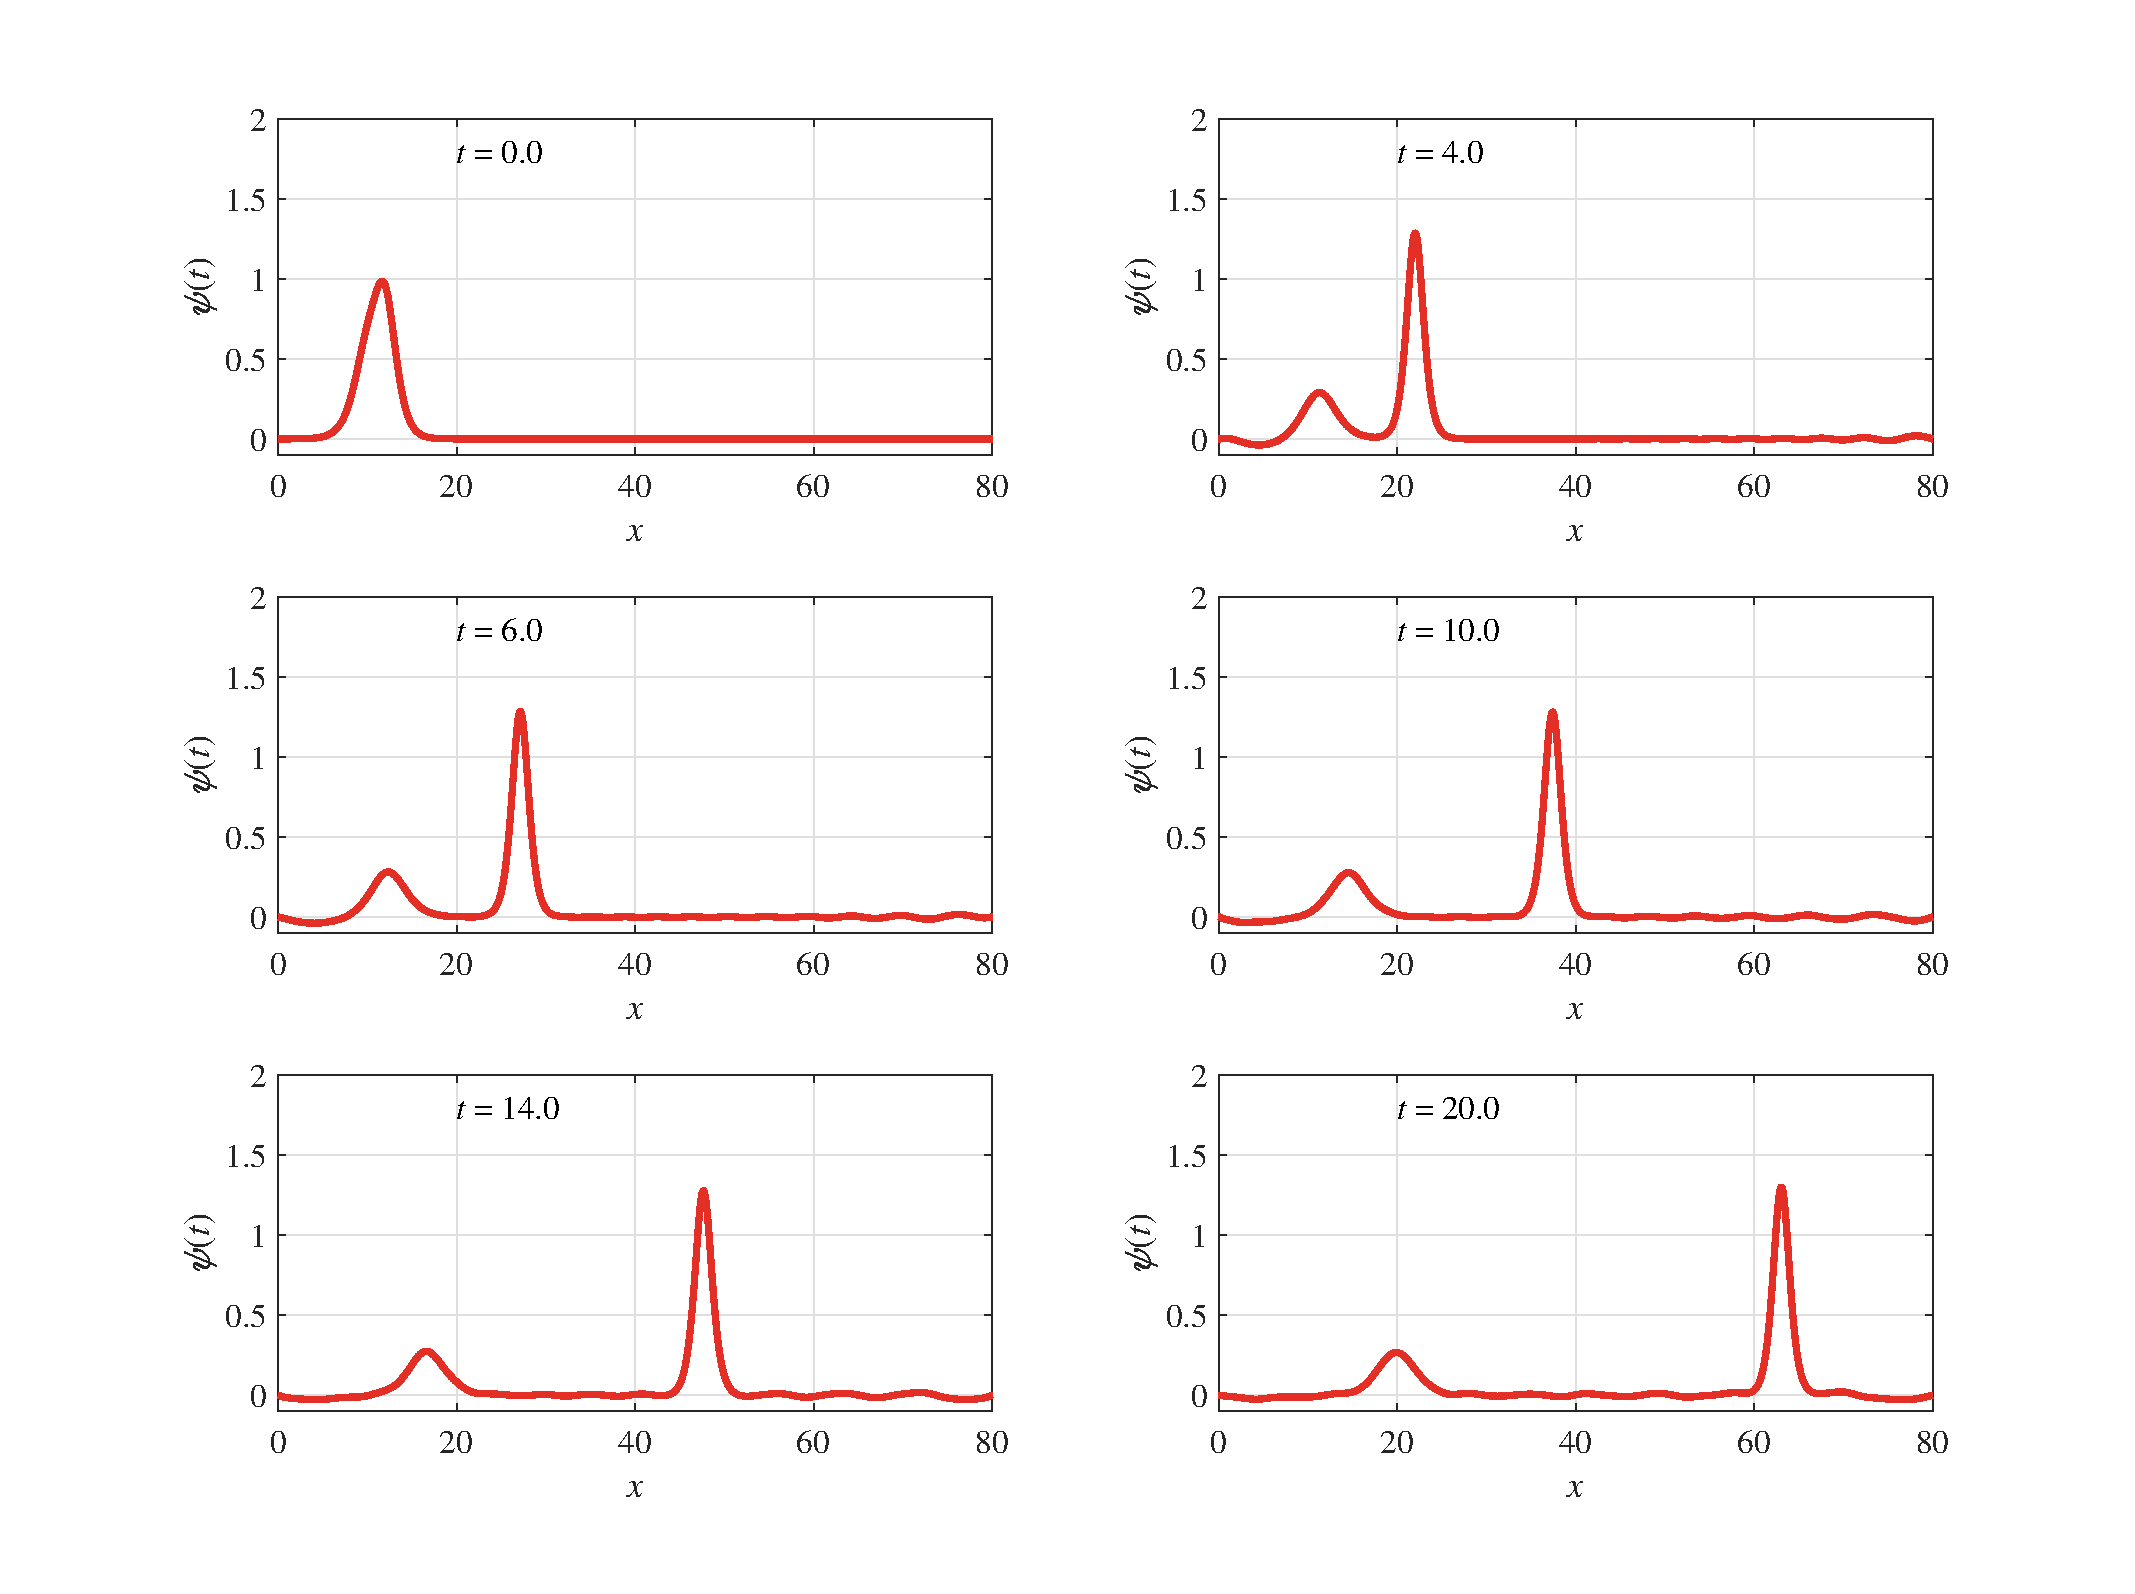
\includegraphics[width=\textwidth]{KdVSolitonSumme1.pdf}
    \caption[Ausbreitung einer Summe aus einzelnen, aber �bereinander liegenden
    Soliton-L�sungen der Korteweg-de-Vries-Gleichung.]
    {Ausbreitung einer Summe aus einzelnen, aber �bereinander liegenden
      Soliton-L�sungen der Korteweg-de-Vries-Gleichung. Die Ausrbreitung
      erfolgt mit unerwarteten Geschwindigkeiten und es sind Deformationionen
      zu erkennen.}
    \label{abb:kontmech_KdVSolitonSumme1}
  \end{figure}

  Diese Summe verh�lt sich ungew�hnlich. Man erkennt zwar nach einiger Zeit,
  dass sich zwei einzelne Soliton-L�sungen zu trennen scheinen, diese breiten
  sich aber nicht mit den Geschwindigkeiten $c=1$ und $c=1.5$ aus, die
  f�r die urspr�ngliche Summe angesetzt waren. Zus�ztlich scheinen
  wellenf�rmige St�rungen mit kleiner Amplitude aufzutreten. Tats�chlich
  scheint die Propagation in der KdV-Gleichung zu sehr vielen soliton-�hnlichen
  Erhebungen zu f�hren, die sich alle mit unterschiedlicher Geschwindigkeit
  ausbreiten. Zus�tzliche St�rungen enstehen hier, da diese St�rungen an den
  R�ndern des endlichen Gitters reflektiert werden, was ein Artefakt der
  numerischen L�sung ist.

  Eine Summe aus zwei Soliton-L�sungen kann allerdings auch eine gute
  N�herung einer exakten L�sung der Korteweg-de-Vries-Gleichung sein. Das
  ist dann der Fall, wenn sich die beiden Solitonen kaum �berschneiden. Dies
  kann man bereits an den Gleichungen \eqref{eq:kontmech_KdVSumme1} bzw.
  \eqref{eq:kontmech_KdVSumme2} erkennen. Ist immer eine der Wellenfunktionen
  und ihre erste $x$-Ableitung Null, so verschwindet auch der st�rende Term.
  In der numerischen L�sung dr�ckt sich das darin aus, dass beide Solitonen
  aus der Summe so in der KdV-Gleichung propagieren, wie man es von ihnen
  erwartet. 

  \begin{figure}
    \centering
    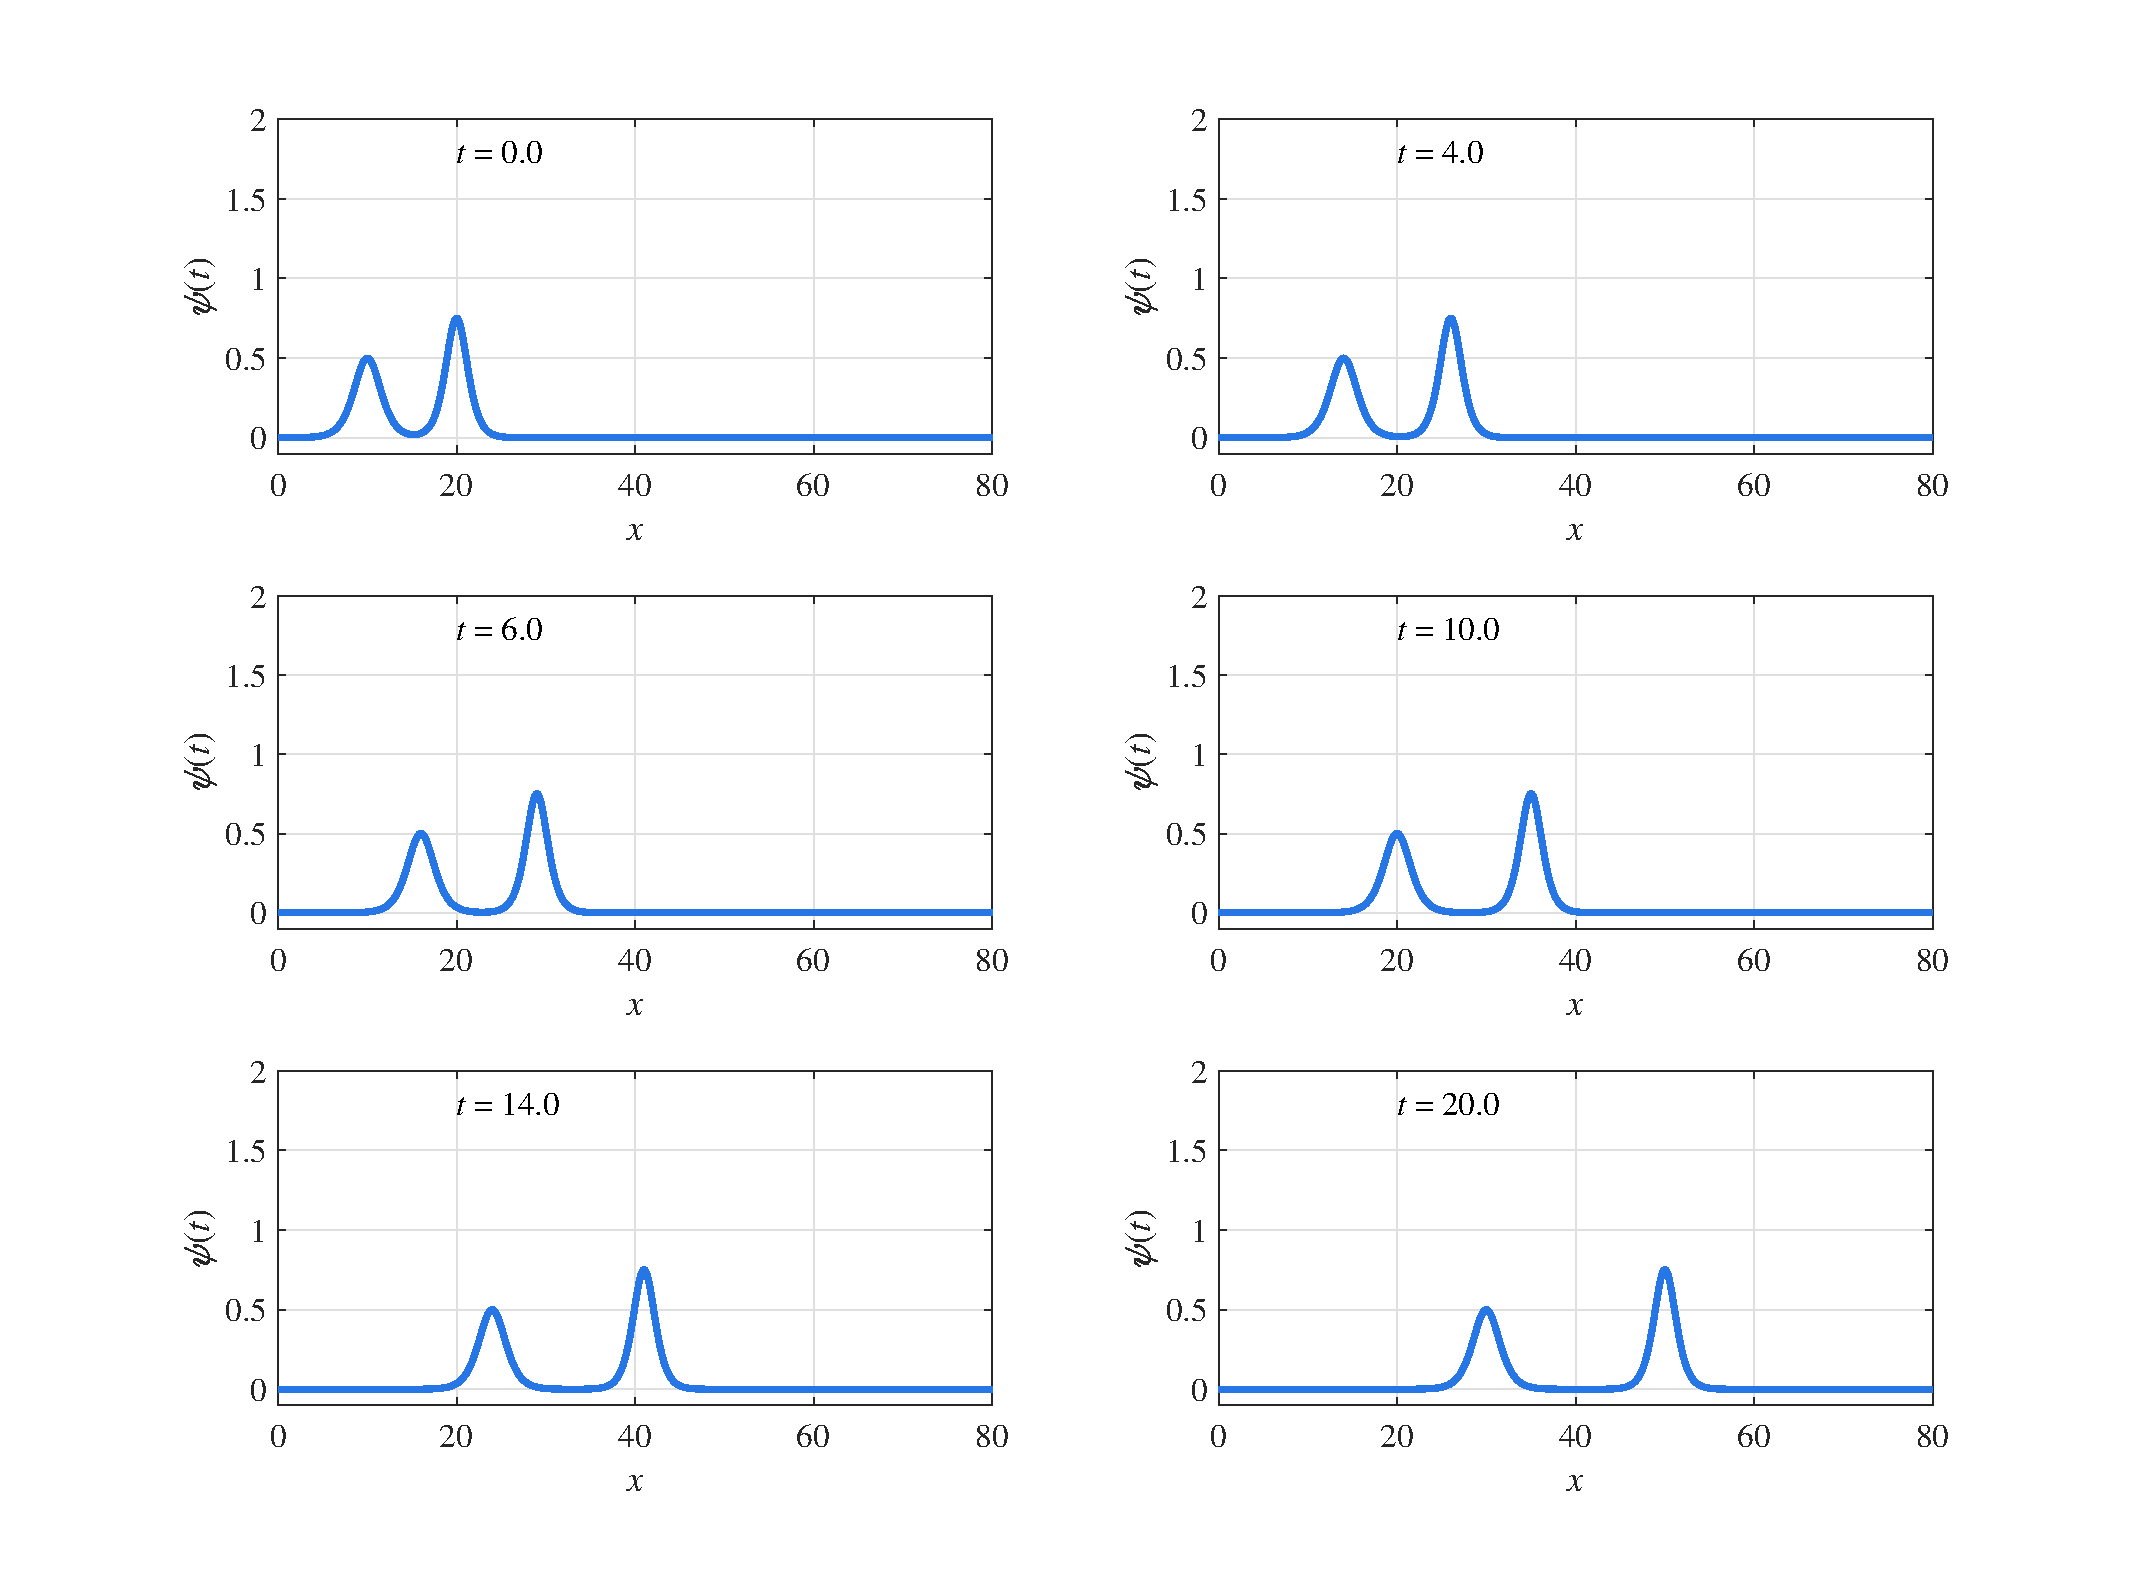
\includegraphics[width=\textwidth]{KdVSolitonSumme2.pdf}
    \caption[Ausbreitung einer Summe aus einzelnen, nicht �bereinander liegenden
    Soliton-L�sungen der Korteweg-de-Vries-Gleichung.]
    {Ausbreitung einer Summe aus einzelnen, nicht �bereinander liegenden
      Soliton-L�sungen der Korteweg-de-Vries-Gleichung. Die Ausbreitung ist
      in der graphischen Darstellung nicht von der von zwei einzelnen Solitonen
      zu unterscheiden.}
    \label{abb:kontmech_KdVSolitonSumme2}
  \end{figure}

  Als Beispiel ist in \figref{kontmech_KdVSolitonSumme2} eine solche Summe
  dargestellt.  Die Anfangsbedingung enth�lt erneut eine Summe aus zwei
  Solitonen mit den Geshwindigkeitsparametern $c=1$ und $c=1.5$. Dabei wurde
  in der Summe das zweite Soliton mit $c=1.5$ deutlich rechts vom ersten
  angesetzt. Zum Beginn der Propagation tritt es erst dort auf, wo das erste
  schon (numerisch) auf Null abgefallen ist. Tatschlich ergibt sich eine
  Propagation, wie wir sie f�r zwei getrennte Soliton-L�sungen mit genau diesen
  Geschwindigkeiten erwarten.

\item Um die Interaktion von zwei Solitonen zu betrachten, l�sen wir wieder
  die Korteweg-de-Vries-Gleichung mit einer Einfangsbedingung, die zwei
  r�umlich getrennte Solitonen enth�lt. Eine solche Situation wird mit einem
  Programm aus der \matlab{}-Datei \mlkontmechref{KdV04.m} gel�st. Das
  Ergebnis ist in \figref{kontmech_KdVSolitonInteraktion} dargestellt. Die
  Anfangsbedingung zur Zeit $t=0$ enth�lt eine �berlagerung aus zwei nach
  rechts laufenden Solitonen mit den Geschwindigkeitsparamtern $c=1$ und
  $c=2$, wobei das schnellere Soliton links vom langsameren ist (dicke
  blaue Linien). Im Zeitverlauf "`�berholt"' es das langsamere Soliton und es
  kommt zur Interaktion. Anschlie�end trennen sie sich wieder und beide
  Solitonen bewegen sich fast so fort, wie sie es ohne Interaktion getan
  h�tten. Einziger Unterschied ist eine Phasenverschiebung $\Delta x$, also
  eine Verschiebung gegen�ber der erwarteten Position ohne Interaktion.

  \begin{figure}
    \centering
    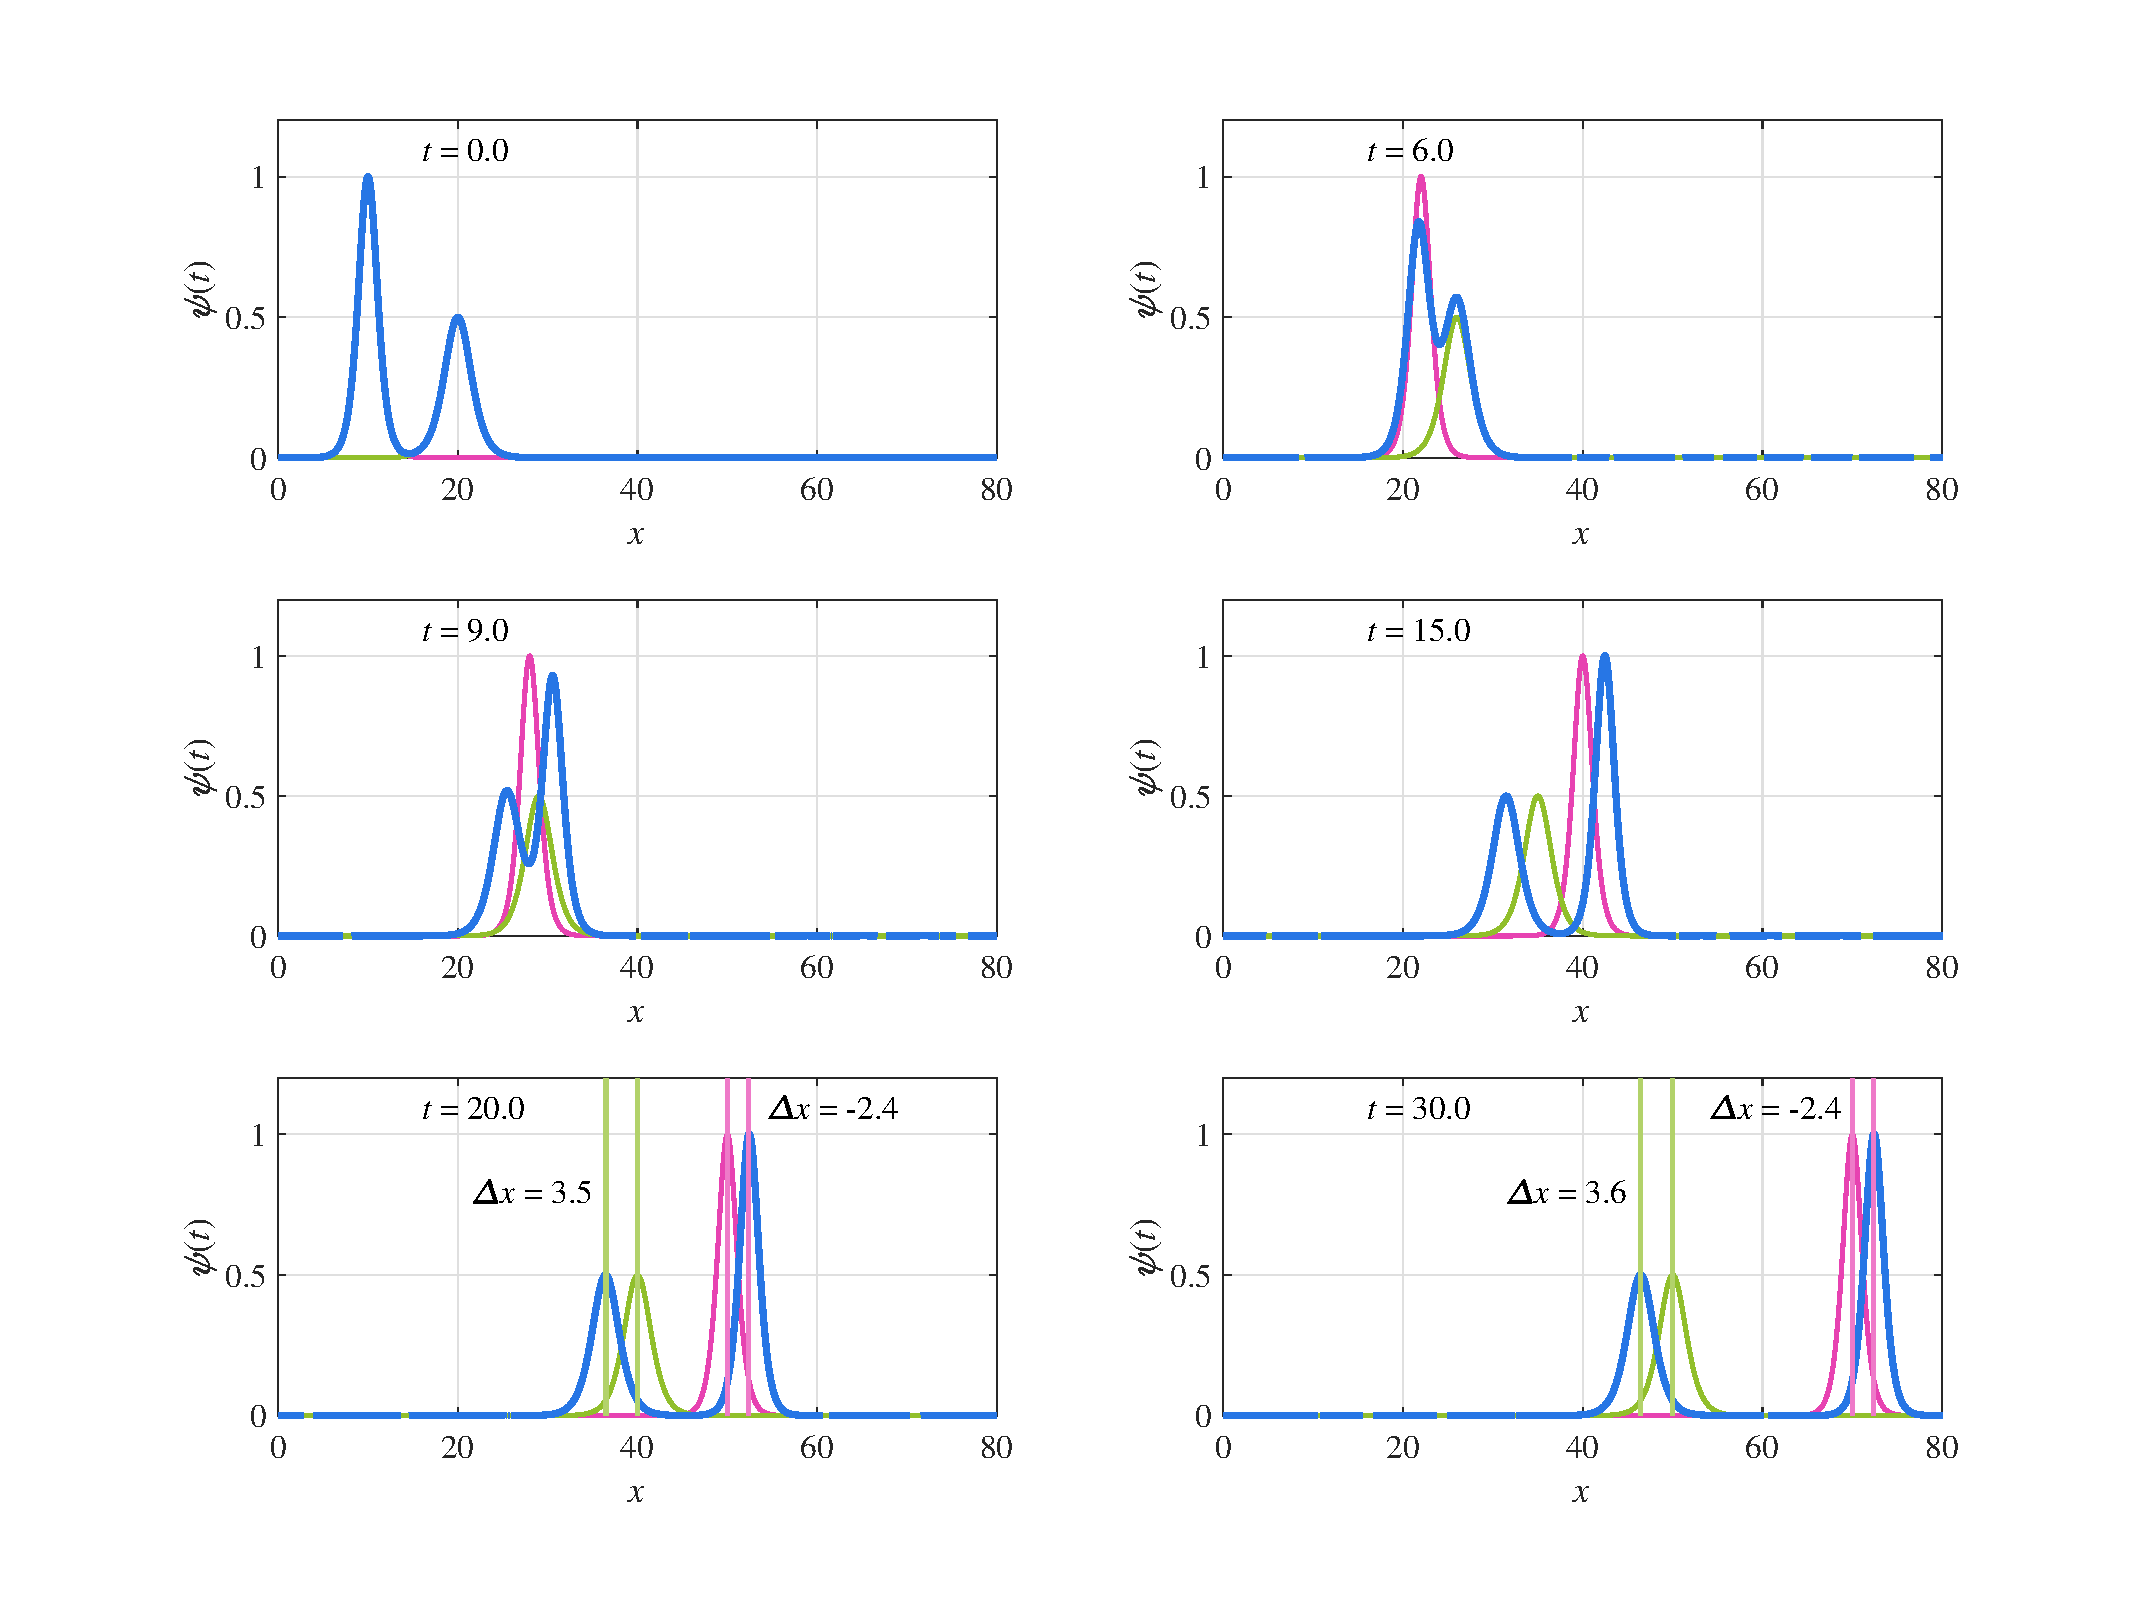
\includegraphics[width=\textwidth]{KdVSolitonInteraktion.pdf}
    \caption[Interaktion zwischen zwei Solitonen der
    Korteweg-de-Vries-Gleichung.]{Nach der Interaktion zwischen zwei Solitonen
      der Korteweg-de-Vries-Gleichung (dicke blaue Linien) ergibt sich eine
      Phasenverschiebung $\Delta x$ geben�ber einzelnen Soliton-L�sungen, die
      sich ungest�rt ausbreiten (d�nne Linien).}
    \label{abb:kontmech_KdVSolitonInteraktion}
  \end{figure}
  
  Um diese Phasenverschiebung bestimmen zu k�nnen, tragen wir ebenfalls die
  analytischen L�sungen f�r zwei einzelne Solitionen auf (d�nne Linien, gr�n
  zu $c=1$, magenta zu $c=2$), die zu $t=0$ mit  der blauen Linie
  �bereinstimmen. Bereits w�hrend der Interaktion sieht man Unterschiede,
  die sich nach der Interaktion zu einem festen Abstand zwischen ungest�rter
  L�sung und L�sung mit Interaktion ergeben. Diese Abst�nde lassen sich durch
  Ausmessen des Abstands bestimmen. Dies geschieht im Programm, indem die
  Position der Maxima der numerischen L�sung ermittelt wird. Ihre Differenz
  zu erwarteten Position der analytischen L�sung
  \begin{equation}
    \Delta x = x_\text{analytisch} - x_\text{numerisch mit Interaktion}
  \end{equation}
  l�sst sich daraus berechnen. Dies geschieht f�r zwei verschiedene Zeiten
  $t$ und man findet:\\

  \begin{tabular}{lll}
    Zeit & Soliton mit $c=1$ & Soliton mit $c=2$ \\
    \hline
    $t=20$ & $\Delta x = 3.5$ & $\Delta x = -2.4$ \\
    $t=30$ & $\Delta x = 3.6$ & $\Delta x = -2.4$ \\
  \end{tabular}\\

  Dies entspricht einem konstanten Abstand nach der Interaktion. Die kleine
  Abweichung f�r das $c=1$-Soliton l�sst sich mit der numerischen Aufl�sung
  erkl�ren. In der numerischen Rechnung haben zwei Gitterpunkte gerade den
  Abstand $0.1$.
\end{enumerate}

\end{sol} 
\textcolor{blue} {$\rightarrow$ zur} \probref{kontmech_soliton1}.\\
\noindent\rule[1ex]{\textwidth}{0.5pt}  \newpage  \clearpage

%-----------------------------------------------------------------------------------------------------------

\begin{sol}{prob:kontmech_soliton2}\label{lsg:kontmech_soliton2} %�bung27
\textbf{Solitonen II}\\ \\

Wir gehen sowohl analytische als auch numerische L�sungen der Solitonen-Typen
beider Gleichungen durch. Um die �bersichtlichkeit zu wahren gehen wir zun�chst
auf die L�sungen der Sinus-Gordon-Gleichung und danach auf die der nichtlinearen
Schr�dingergleichung ein. Am Ende folgt ein Vergleich der Solitonen beider
Gleichungen.

Zun�chst wollen wir die analtyisch gegebenen Solitonen 
\begin{equation}
  \psi(x,t) = 4 \arctan \lk \mathrm{exp}\lek \pm \frac{x-vt}{\sqrt{1-(v/c)^2}}
  \rek \rk
  \tag{\ref{eq:kontmech_soliton04}}
\end{equation}
f�r verschiedene Parameter darstellen. Diese sind in
\figref{kontmech_SinusGordon1} gegeben.

\begin{figure}
  \centering
  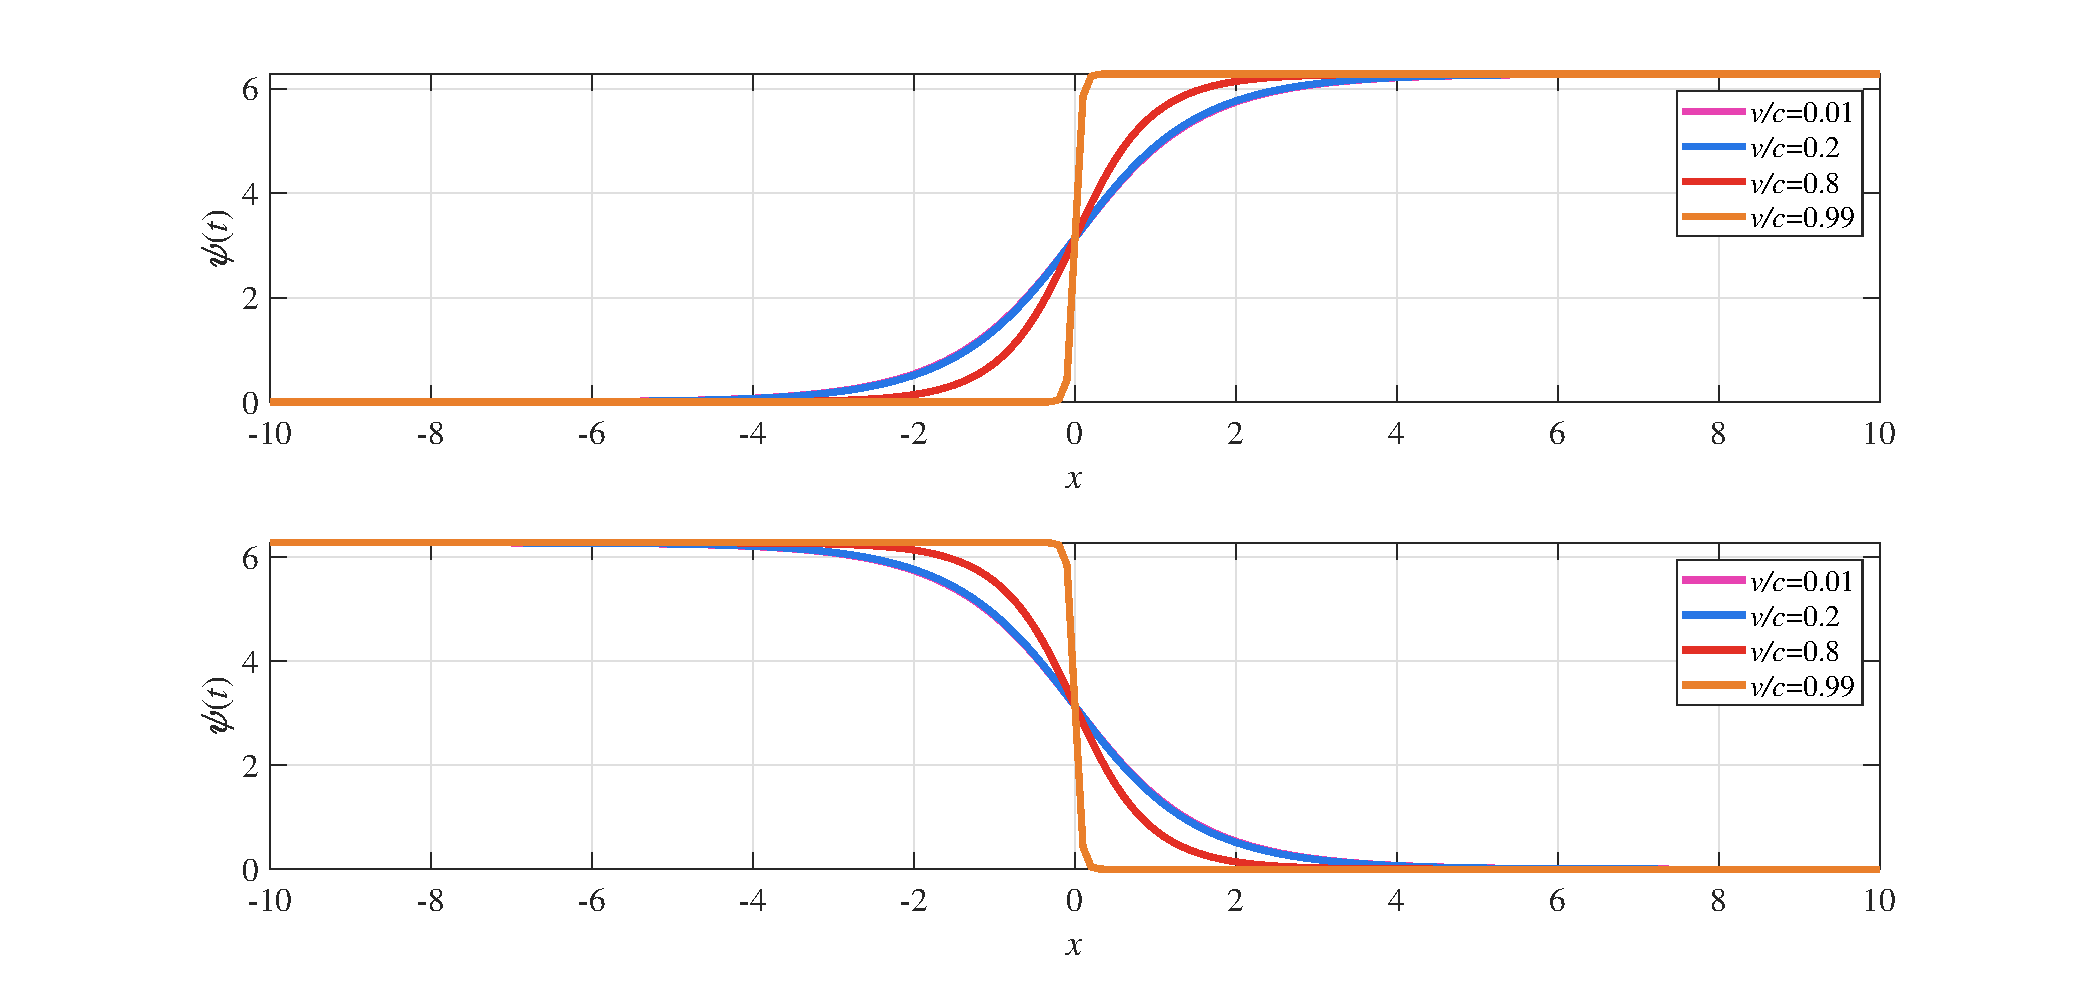
\includegraphics[width=\textwidth]{SinusGordon1.pdf}
  \caption[L�sungen der Sinus-Gordon-Gleichung bei Variation der
  Parameter]{L�sungen der Sinus-Gordon-Gleichung bei Variation der
    Parameter, wobei ausschlie�lich das Verh�ltnis $v/c$ ausschlaggebend ist.}
  \label{abb:kontmech_SinusGordon1}
\end{figure}

Die Form h�ngt dabei nur vom Verh�ltnis $v/c$ ab, da die Geschwindigkeit $v$
allein ausschlie�lich einen Einfluss auf die Fortbewegung des Solitons hat.
Sie besteht aus einer ansteigenden Stufe f�r den ersten Typ mit dem Vorzeichen
$+$ im Exponenten (kink) bzw. einer absteigenden Stufe f�r das Vorzeichen $-$
(anti-kink). Je gr��er das Verh�ltnis ist, desto steiler steigt die Stufe an
bzw. desto steiler f�llt sie ab.

Die Fortbewegung ist in \figref{kontmech_SinusGordon2} dargestellt. Die Form
bleibt bei der Propagation erhalten und es gibt eine exakte �bereinstimmung
der numerischen L�sung der partiellen Differentialgleichung mit der
Methode der finiten Differenzen (dick gestrichelte Linien) mit der analytischen
L�sung (d�nne durchgezogene Linien). Dies zeigt, dass hier tats�chlich
Solitonen vorliegen, die mit unver�nderter Form nach rechts propagieren.

\begin{figure}
  \centering
  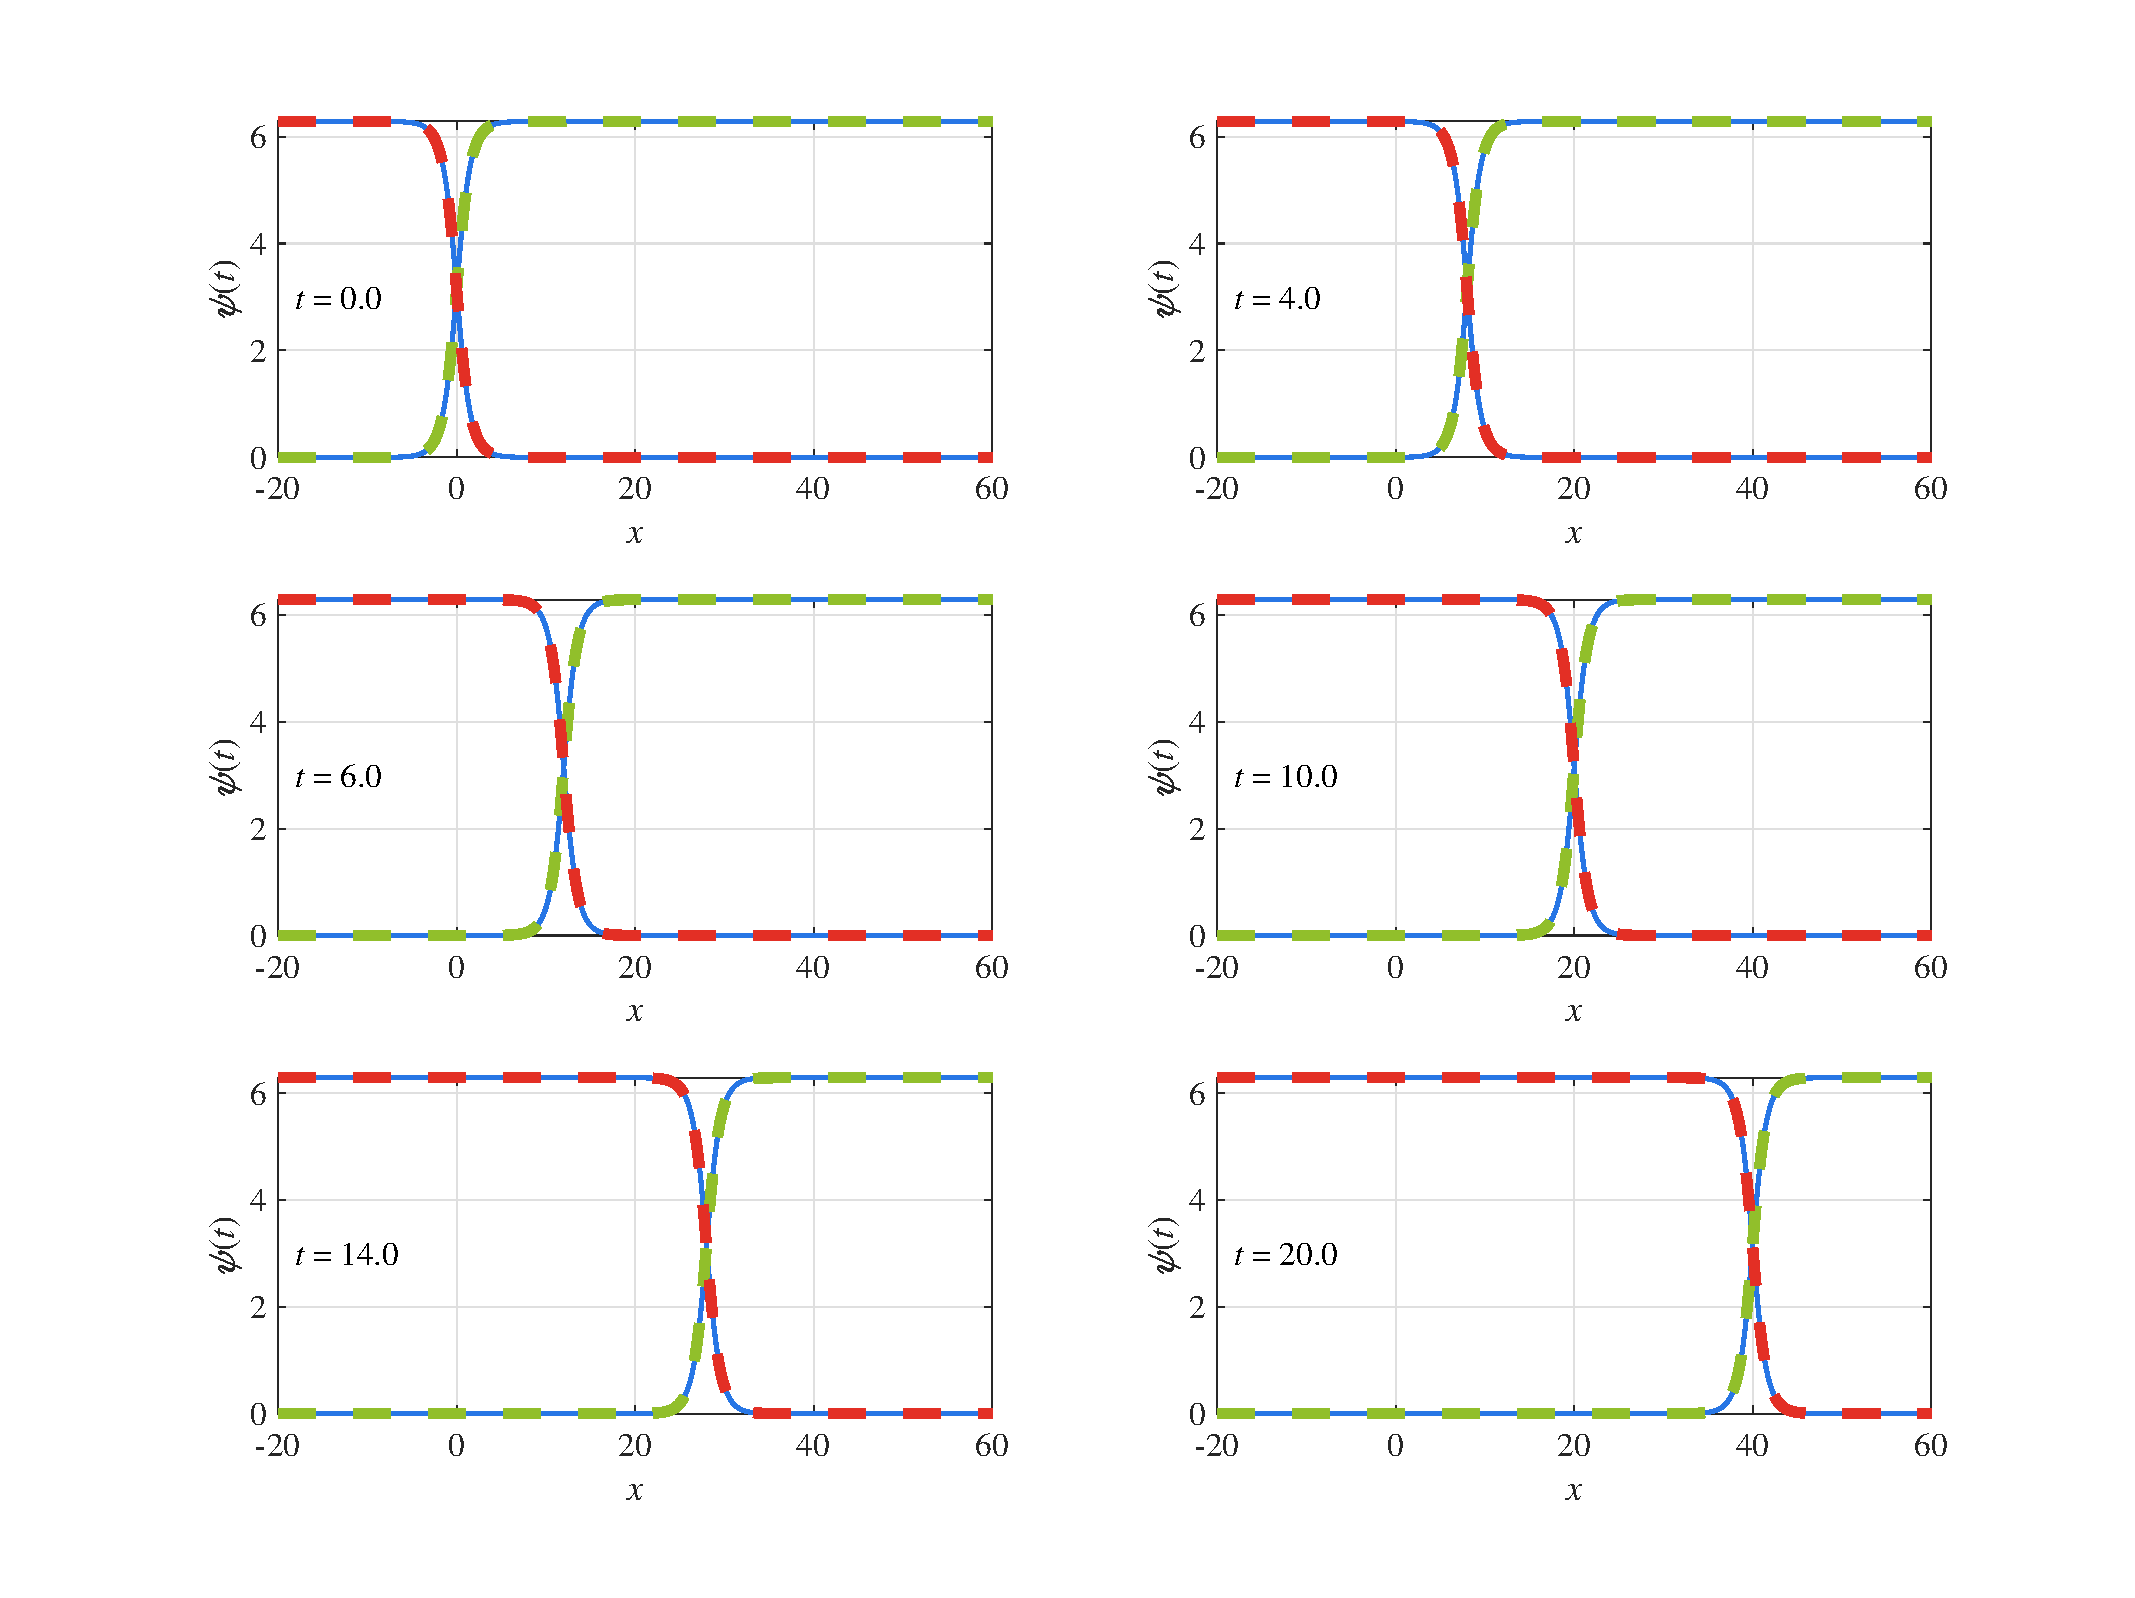
\includegraphics[width=\textwidth]{SinusGordon2.pdf}
  \caption[Numerische L�sungen der Sinus-Gordon-Gleichung]{Numerische
    L�sungen der Sinus-Gordon-Gleichung mit einer Geschwindigkeit $v = 2$
    bei einer Maximalgeschwindigkeit von $c = 10$. Die numerische Intergration
    mit der Methode der finiten Differenzen (dick gestrichelte Linien) stimmt
    exakt mit der analytischen Form (d�nne durchgezogene Linien) �berein.}
  \label{abb:kontmech_SinusGordon2}
\end{figure}

Es l�sst sich selbstverst�ndlich auch analytisch zeigen, dass die Funktionen
\eqref{eq:kontmech_soliton04} L�sungen der Sinus-Gordon-Gleichung
\begin{equation}
  \frac{1}{c^2}\frac{\partial^2 \psi}{\partial t^2}
  - \frac{\partial^2 \psi}{\partial x^2}  + \sin \psi = 0
  \tag{\ref{eq:kontmech_soliton03}}
\end{equation}
sind. Dazu berechnen wir zun�chst die ben�tigten Ableitungen. Diese sind
\begin{subequations}
  \allowdisplaybreaks
  \begin{align}
    \frac{\partial \psi}{\partial t}
    &= \frac{\mp 4\, v}{\sqrt{1-(v/c)^2}}
      \frac{\exp \lek \pm \frac{x-vt}{\sqrt{1-(v/c)^2}} \rek}
      {1+\exp \lek \pm 2\, \frac{x-vt}{\sqrt{1-(v/c)^2}} \rek} \; , \\
    \frac{\partial^2 \psi}{\partial t^2}
    &= \frac{4\, v^2}{1-(v/c)^2}
      \frac{\exp \lek \pm \frac{x-vt}{\sqrt{1-(v/c)^2}} \rek}
      {1+\exp \lek \pm 2\, \frac{x-vt}{\sqrt{1-(v/c)^2}} \rek} \lk 1 -
      \frac{2 \exp \lek \pm 2\, \frac{x-vt}{\sqrt{1-(v/c)^2}} \rek}
      {1+\exp \lek \pm 2\, \frac{x-vt}{\sqrt{1-(v/c)^2}} \rek} \rk  \notag \\
    &= \frac{4\, v^2}{1-(v/c)^2}
      \frac{\exp \lek \pm \frac{x-vt}{\sqrt{1-(v/c)^2}} \rek}
      {1+\exp \lek \pm 2\, \frac{x-vt}{\sqrt{1-(v/c)^2}} \rek} 
      \frac{1- \exp \lek \pm 2\, \frac{x-vt}{\sqrt{1-(v/c)^2}} \rek}
      {1+\exp \lek \pm 2\, \frac{x-vt}{\sqrt{1-(v/c)^2}} \rek} \notag \\
    &= \frac{4\, v^2}{1-(v/c)^2}
      \frac{\exp \lek \pm \frac{x-vt}{\sqrt{1-(v/c)^2}} \rek -
      \exp \lek \pm 3\, \frac{x-vt}{\sqrt{1-(v/c)^2}} \rek}
      {\lk 1+\exp \lek \pm 2\, \frac{x-vt}{\sqrt{1-(v/c)^2}} \rek \rk^2} \; , \\
    \frac{\partial \psi}{\partial x} 
    &= \frac{\pm 4}{\sqrt{1-(v/c)^2}}
      \frac{\exp \lek \pm \frac{x-vt}{\sqrt{1-(v/c)^2}} \rek}
      {1+\exp \lek \pm 2\, \frac{x-vt}{\sqrt{1-(v/c)^2}} \rek} \; , \\
    \frac{\partial^2 \psi}{\partial x^2}
    &= \frac{4}{1-(v/c)^2}
      \frac{\exp \lek \pm \frac{x-vt}{\sqrt{1-(v/c)^2}} \rek -
      \exp \lek \pm 3\, \frac{x-vt}{\sqrt{1-(v/c)^2}} \rek}
      {\lk 1+\exp \lek \pm 2\, \frac{x-vt}{\sqrt{1-(v/c)^2}} \rek \rk^2} \; .
  \end{align}
\end{subequations}
F�r die Sinusfunktion in der Differentialgleichung verwenden wir die
Additionstheoreme
\begin{equation*}
  \sin x = \frac{2\tan(x/2)}{1+\tan^2(x/2)} \qquad \text{sowie}
  \qquad \tan x = \frac{2\tan(x/2)}{1-\tan^2(x/2)} 
\end{equation*}
und setzen sie ineinander ein
\begin{equation*}
  \sin x = \frac{2 \frac{2\tan(x/4)}{1-\tan^2(x/4)} }{1 +
    \lk \frac{2\tan(x/4)}{1-\tan^2(x/4)} \rk^2}
  = 4 \, \frac{\tan(x/4) - \tan^3(x/4)}{\lk 1 + \tan^2(x/4) \rk^2} \; .
\end{equation*}
Damit erhalten wir
\begin{multline*}
  \frac{1}{c^2}\frac{\partial^2 \psi}{\partial t^2}
  - \frac{\partial^2 \psi}{\partial x^2}  + \sin \psi
  = \frac{1}{c^2} \frac{4\, v^2}{1-(v/c)^2}
      \frac{\exp \lek \pm \frac{x-vt}{\sqrt{1-(v/c)^2}} \rek -
      \exp \lek \pm 3\, \frac{x-vt}{\sqrt{1-(v/c)^2}} \rek}
    {\lk 1+\exp \lek \pm 2\, \frac{x-vt}{\sqrt{1-(v/c)^2}} \rek \rk^2} \\
    - \frac{4}{1-(v/c)^2}
      \frac{\exp \lek \pm \frac{x-vt}{\sqrt{1-(v/c)^2}} \rek -
      \exp \lek \pm 3\, \frac{x-vt}{\sqrt{1-(v/c)^2}} \rek}
    {\lk 1+\exp \lek \pm 2\, \frac{x-vt}{\sqrt{1-(v/c)^2}} \rek \rk^2}
    + 4\, \frac{\tan(\psi/4) - \tan^3(\psi/4)}{\lk 1 + \tan^2(\psi/4) \rk^2} \\
    = - 4 \frac{\exp \lek \pm \frac{x-vt}{\sqrt{1-(v/c)^2}} \rek -
      \exp \lek \pm 3\, \frac{x-vt}{\sqrt{1-(v/c)^2}} \rek}
    {\lk 1+\exp \lek \pm 2\, \frac{x-vt}{\sqrt{1-(v/c)^2}} \rek \rk^2}
    + 4\, \frac{\exp \lek \pm \frac{x-vt}{\sqrt{1-(v/c)^2}} \rek
      - \exp \lek \pm 3\, \frac{x-vt}{\sqrt{1-(v/c)^2}} \rek}
    {\lk 1 + \exp \lek \pm 2\, \frac{x-vt}{\sqrt{1-(v/c)^2}} \rek \rk^2}
    = 0 \; ,
\end{multline*}
was best�tigt, dass die Differentialgleichung von der Funktion
\eqref{eq:kontmech_soliton04} erf�llt wird. Somit haben wir gezeigt, dass
tats�chlich analytisch bekannte Solitonen der Sinus-Gordon-Gleichung
vorliegen.

F�r eine numerische L�sung der partiellen Differentialgleichung mit der
Methode der finiten Differenzen geben wir zun�chst wieder die diskretisierten
Ableitungen an. Wir ben�tigen f�r die Sinus-Gordon-Gleichung
\eqref{eq:kontmech_soliton03} die zweiten Ableitungen nach der Zeit und dem
Ort,
\begin{subequations}
  \begin{align}
    \frac{\partial^2 \psi(x_i,t_j)}{\partial t^2}
    &= \frac{\psi(x_{i},t_{j+1}) + \psi(x_{i},t_{j-1}) -2 \psi(x_{i},t_{j})}
      {\Delta t^2}  \; , \\
    \frac{\partial^2 \psi(x,t)}{\partial x^2}
    &= \frac{\psi(x_{i+1},t_{j}) + \psi(x_{i-1},t_{j}) -2 \psi(x_{i},t_{j})}
      {\Delta x^2}  \; .
  \end{align}
\end{subequations}
Mit diesen l�sst sich die Sinus-Gordon-Gleichung diskret schreiben als
\begin{subequations}
  \begin{multline}
    \frac{1}{c^2} \frac{\psi(x_{i},t_{j+1}) + \psi(x_{i},t_{j-1})
      -2 \psi(x_{i},t_{j})}{\Delta t^2}
    - \frac{\psi(x_{i+1},t_{j}) + \psi(x_{i-1},t_{j}) -2 \psi(x_{i},t_{j})}
    {\Delta x^2} \\
    + \sin\psi\lk \psi(x_{i},t_{j}) \rk = 0 \; ,
  \end{multline}
  was sich zum Interrationsschritt
  \begin{multline}
    \psi(x_{i},t_{j+1}) = 2 \psi(x_{i},t_{j}) - \psi(x_{i},t_{j-1})
    + c^2 \frac{\Delta t^2}{\Delta x^2} \left ( \psi(x_{i+1},t_{j})
      + \psi(x_{i-1},t_{j}) -2 \psi(x_{i},t_{j}) \right ) \\
    - c^2 \, \Delta t^2\, \sin\lk \psi(x_{i},t_{j}) \rk 
  \end{multline}
\end{subequations}
f�r die Methode der finiten Differenzen aufl�sen l�sst.
Diese Berechnung wird in einem Programm in der \matlab{}-Datei
\mlkontmechref{SinusGordonSolitonen.m} durchgef�hrt.


Vollkommen analog gehen wir f�r die nichtlineare Schr�dinger-Gleichung vor.
zun�chst stellen wir die Fundamentall�sung
\begin{align}
  \psi(x,t) = A_0\;\sech \lk \frac{t- x/v }{\tau_0} \rk \mathrm{exp}\lek
  -\im \frac{x}{x_0} \rek
  \tag{\ref{eq:kontmech_soliton06}}
\end{align}
f�r verschiedene Parameter $v$ und $g$ dar. Die L�sungen k�nnen in
\figref{kontmech_NLSG1} gefunden werden.

\begin{figure}
  \centering
  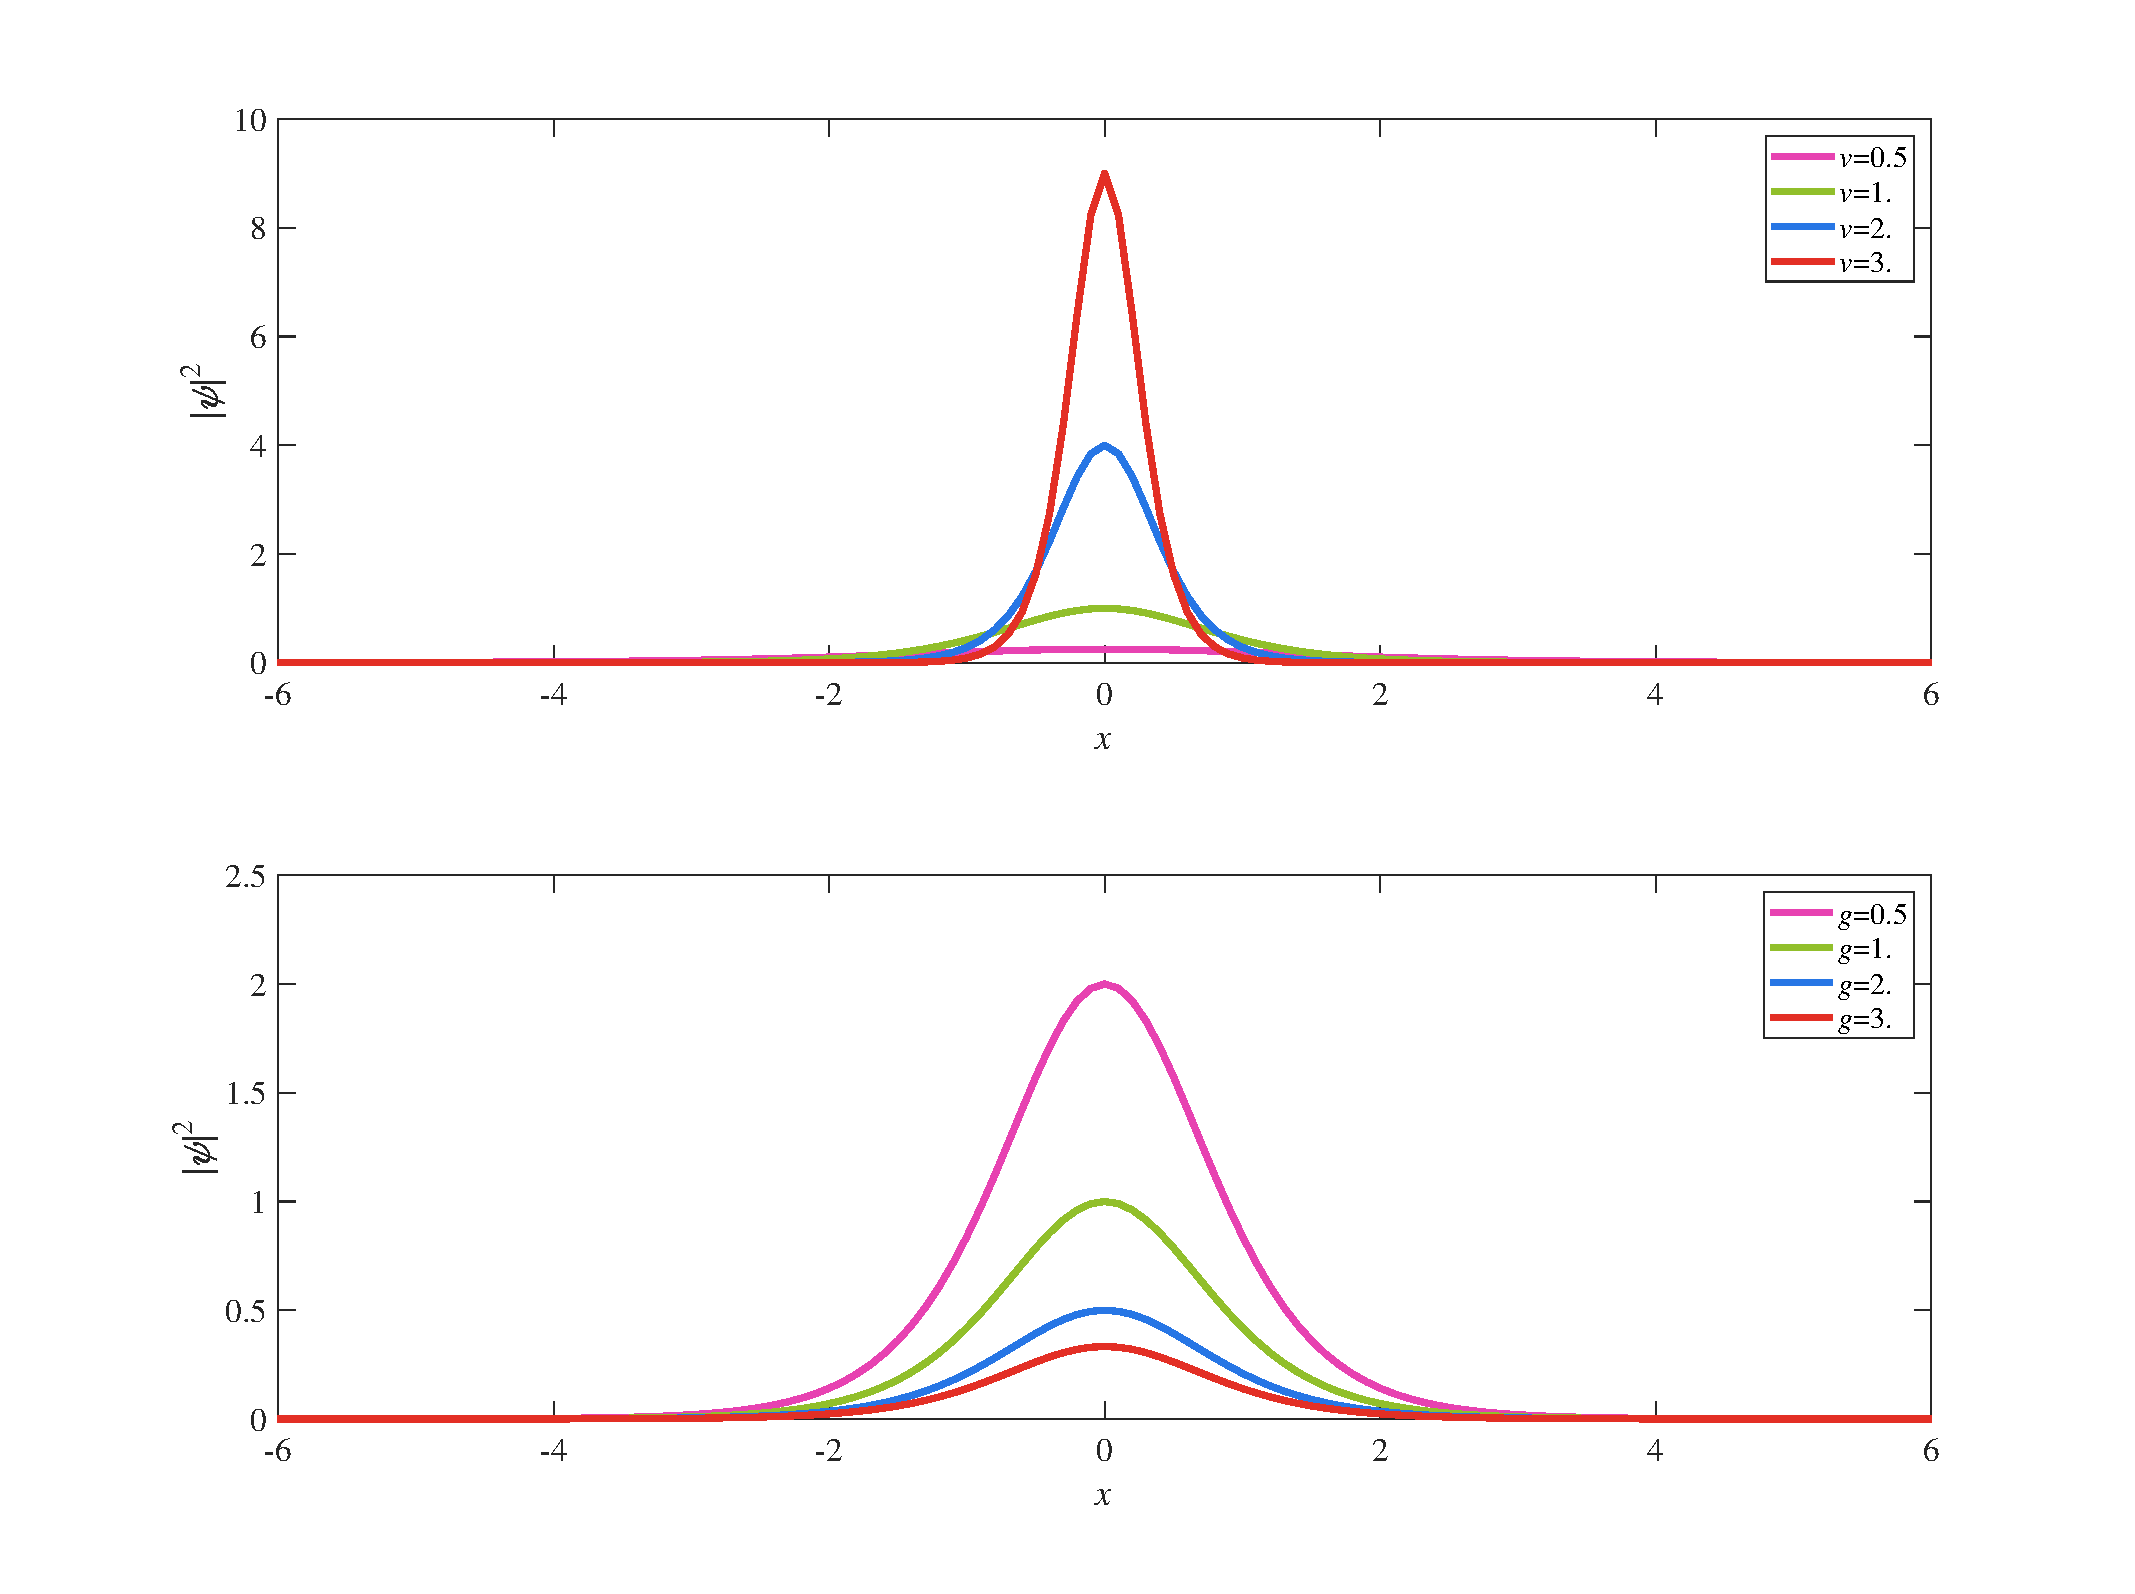
\includegraphics[width=\textwidth]{NLSGSolitonen_1.pdf}
  \caption[L�sungen der nichtlinearen Schr�dinger-Gleichung bei Variation der
  Parameter]{L�sungen der nichtlinearen Schr�dinger-Gleichung f�r verschiedene
    Parameter $v$ und $g$.}
  \label{abb:kontmech_NLSG1}
\end{figure}

Das Soliton steigt um sein Zentrum an und f�llt danach wieder auf den Wert
Null ab.  Die Parameter $v$ und $g$ k�nnen unabh�ngig von einander variiert
werden und haben unterschiedliche Auswirkungen. Gemeinsam ist beiden, dass sie
sehr stark die Amplitude ver�ndern, was f�r die nichtlineare Gleichung zu
erwarten ist. Dabei zeigt sich, dass kleine Werte $v$ zu einem breiten und
flachen Soliton f�hren, gro�e werte zu einem steilen und hohen. Variiert man
den Parameter $g$, der die St�rke der Nichtlinearit�t ausdr�ckt, so findet
man f�r kleine Werte von $g$ ein hohes Soliton, f�r gro�e ein niedriges.

Die Propagation eines Solitons f�r die Parameter $v = 1.5$ und
$g = 0.8$ ist in \figref{kontmech_NLSG2} zu sehen. Die numerische L�sung
(dick gestrichelte Linien) f�hrt auf ein Soliton, das sich in seiner Form und
Gr��e nicht �ndert, sondern ausschlie�lich mit dem Geschwindigkeit $v$ nach
rechts propagiert. Dabei zeigt es f�r jeden Zeitschritt eine sehr gute
�bereinstimmung mit der analytsischen Erwartung \eqref{eq:kontmech_soliton06}.

\begin{figure}
  \centering
  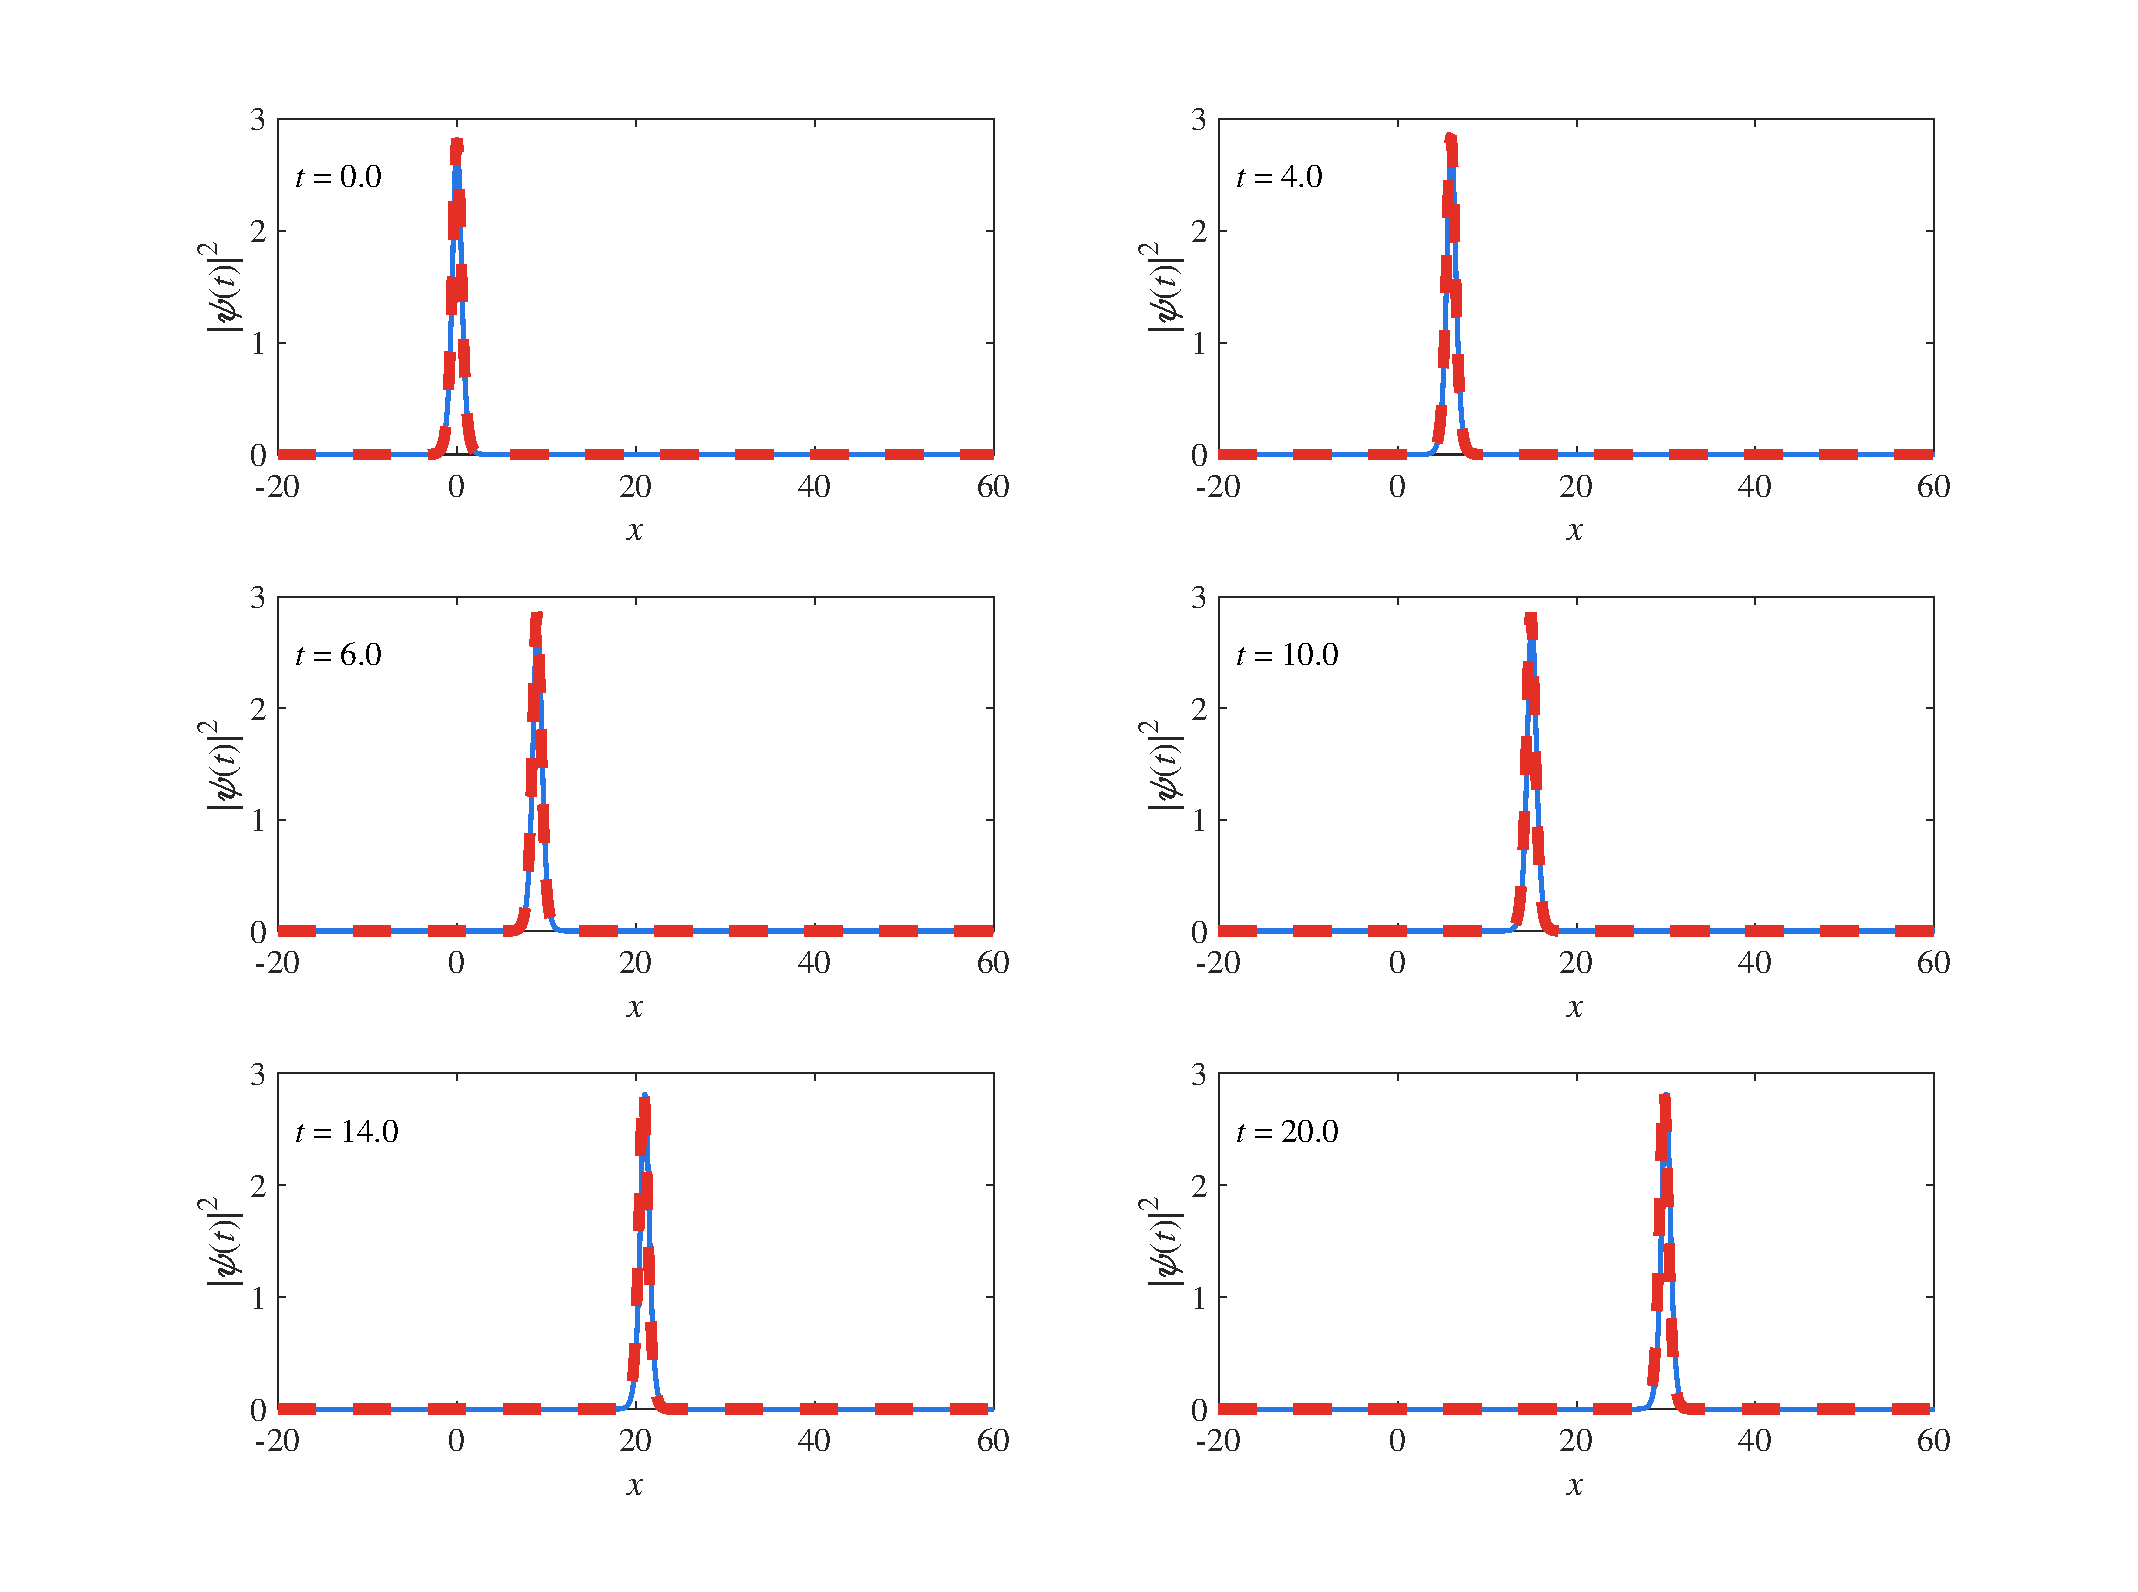
\includegraphics[width=\textwidth]{NLSGSolitonen_2.pdf}
  \caption[Numerische L�sungen der nichtlinearen Schr�dinger-Gleichung]
  {Numerische L�sungen der nichtlinearen Schr�dinger-Gleichung f�r die
    Propagation eines Solitons mit dem Parametern $v = 1.5$ und $g = 0.8$.
    Die Form bleibt erhalten und die numerische Intergration mit der Methode
    der finiten Differenzen (dick gestrichelte Linien) stimmt exakt mit der
    analytischen Form (d�nne durchgezogene Linien) �berein.}
  \label{abb:kontmech_NLSG2}
\end{figure}

Aus dem Vergleich der analytischen und der numersichen L�sung in
\figref{kontmech_NLSG2} k�nnen wir bereits vermuten, dass die analytische
gegebene Funktion \eqref{eq:kontmech_soliton06} eine L�sung der
nichtlinearen Schr�dinger-Gleichung
\begin{equation}
  \im\,\frac{\partial \psi}{\partial t} + \frac{1}{2}\,\frac{\partial^2 \psi}
  {\partial x^2} + g\, \left|\psi\right|^2\,\psi = 0  
  \tag{\ref{eq:kontmech_soliton05}}
\end{equation}
ist. Dies k�nnen und wollen wir nun noch durch eine Rechnung zeigen. Erneut
berechnen wir daf�r zun�chst die ben�tigten Ableitungen,
\begin{subequations}
  \begin{align}
    \frac{\partial \psi(x,t)}{\partial t}
    &= -\frac{A_0}{\tau_0}
      \frac{\sinh\lk \frac{t- x/v}{\tau_0} \rk}{\cosh^2 \lk \frac{t- x/v }
      {\tau_0} \rk} \exp \lek -\im \frac{x}{x_0} \rek \; , \\
    \frac{\partial \psi(x,t)}{\partial x}
    &= \frac{A_0}{v\,\tau_0}
      \frac{\sinh\lk \frac{t- x/v}{\tau_0} \rk}{\cosh^2 \lk \frac{t- x/v }
      {\tau_0} \rk} \exp \lek -\im \frac{x}{x_0} \rek
      - \frac{\im A_0}{x_0} \frac{1}{\cosh \lk \frac{t- x/v}{\tau_0} \rk}
      \exp \lek -\im \frac{x}{x_0} \rek \; , \\
    \frac{\partial^2 \psi(x,t)}{\partial x^2}
    &= -\frac{A_0}{(v\,\tau_0)^2} \frac{1}{\cosh \lk \frac{t- x/v}{\tau_0} \rk}
      \exp \lek -\im \frac{x}{x_0} \rek
      + \frac{2 A_0}{(v\,\tau_0)^2} \frac{\sinh^2\lk \frac{t- x/v}{\tau_0} \rk}
      {\cosh^3 \lk \frac{t- x/v}{\tau_0} \rk} \exp \lek -\im \frac{x}{x_0} \rek
      \notag \\
      &\quad - \frac{2\,\im A_0}{v\,\tau_0\, x_0}
      \frac{\sinh\lk \frac{t- x/v}{\tau_0} \rk}{\cosh^2 \lk \frac{t- x/v }
        {\tau_0} \rk} \exp \lek -\im \frac{x}{x_0} \rek
        - \frac{A_0}{x_0^2} \frac{1}{\cosh \lk \frac{t- x/v}{\tau_0} \rk}
      \exp \lek -\im \frac{x}{x_0} \rek \; .
  \end{align}
\end{subequations}
Eingesetzt in die Differentialgleichung \eqref{eq:kontmech_soliton05}
erh�lt man
\begin{multline}
  -\frac{\im A_0}{\tau_0} \lk 1 + \frac{1}{v\, x_0} \rk
  \frac{\sinh\lk \frac{t- x/v}{\tau_0} \rk}{\cosh^2 \lk \frac{t- x/v }
    {\tau_0} \rk} \exp \lek -\im \frac{x}{x_0} \rek
  + A_0 \Bigg \{ -\frac{1}{2 (v\,\tau_0)^2} \cosh^2 \lk \frac{t- x/v}{\tau_0}
  \rk + \frac{1}{(v\,\tau_0)^2} \sinh^2\lk \frac{t- x/v}{\tau_0} \rk \\
  - \frac{1}{2\, x_0^2} \cosh^2 \lk \frac{t- x/v}{\tau_0} \rk + g |A_0|^2
  \Bigg \}
  \frac{1}{\cosh^3 \lk \frac{t- x/v}{\tau_0} \rk}
  \exp \lek -\im \frac{x}{x_0} \rek = 0 \; .
\end{multline}
Da alle Koeffizienten reell sind und sich die komplexe Exponentialfunktion
k�rzen l�sst, m�ssen relle und imagin�re Vorfaktoren auf der linken Seite
getrennt verschwinden, um die Differentialgleichung erf�llen zu k�nnen. F�r
den imagin�ren Vorfaktor (erster Summand) f�hrt das auf
\begin{subequations}
  \begin{equation}
    x_0 = - \frac{1}{v} \; .
    \label{eq:kontmech_NLSG_par1}
  \end{equation}
  Damit in der geschweiften Klammer keine Funktion mehr vorkommt und die
  Differentialgleichung f�r alle $x$ und $t$ erf�llt sein kann, muss
  \begin{equation}
    \tau_0 = \pm \frac{1}{v^2}
    \label{eq:kontmech_NLSG_par2}
  \end{equation}
  erf�llt sein. Mit diesem $\tau_0$ k�nnen wir
  \begin{multline*}
    -\frac{1}{2 (v\,\tau_0)^2} \cosh^2 \lk \frac{t- x/v}{\tau_0} \rk
    + \frac{1}{(v\,\tau_0)^2} \sinh^2\lk \frac{t- x/v}{\tau_0} \rk
    - \frac{1}{2\, x_0^2} \cosh^2 \lk \frac{t- x/v}{\tau_0} \rk \\
    = -\frac{v^2}{2} \cosh^2 \lk \frac{t- x/v}{\tau_0} \rk
    + v^2 \sinh^2\lk \frac{t- x/v}{\tau_0} \rk
    - \frac{v^2}{2} \cosh^2 \lk \frac{t- x/v}{\tau_0} \rk \\
    = v^2 \Bigg \{ - \cosh^2 \lk \frac{t- x/v}{\tau_0} \rk
    + \sinh^2\lk \frac{t- x/v}{\tau_0} \rk \Bigg \} = -v^2
  \end{multline*}
  zusammenfassen und die gesamte geschweifte Klammer verschwindet f�r
  \begin{equation}
    A_0 = \frac{v}{\sqrt{g}}
    \label{eq:kontmech_NLSG_par3}
  \end{equation}
\end{subequations}
oder jedem komplexen $A_0$ mit demselben Betrag. Damit haben wir aber gezeigt,
dass f�r die gefunden Werte $x_0$, $\tau_0$ und $A_0$ aus den Gleichungen
\eqref{eq:kontmech_NLSG_par1}-\eqref{eq:kontmech_NLSG_par3} die Funktion
\eqref{eq:kontmech_soliton06} eine L�sung der nichtlinearen
Schr�dinger-Gleichung ergibt.

F�r die L�sung mit der Methode der finiten Differenzen  m�ssen wir erneut
die Ableitungen diskretisieren. Ben�tigt werden
\begin{subequations}
  \begin{align}
    \frac{\partial \psi(x_i,t_j)}{\partial t}
    &= \frac{\psi(x_{i},t_{j+1}) - \psi(x_{i},t_{j-1})}{2\Delta t}  \; , \\
    \frac{\partial^2 \psi(x,t)}{\partial x^2}
    &= \frac{\psi(x_{i+1},t_{j}) + \psi(x_{i-1},t_{j}) -2 \psi(x_{i},t_{j})}
      {\Delta x^2}  \; .
  \end{align}
\end{subequations}
Damit l�sst sich die nichtlineare Schr�dinger-Gleichung auf die diskrete Form
\begin{subequations}
  \begin{multline}
    \im \frac{\psi(x_{i},t_{j+1}) - \psi(x_{i},t_{j-1})}{2\Delta t}
    + \frac{1}{2} \frac{\psi(x_{i+1},t_{j}) + \psi(x_{i-1},t_{j})
      -2 \psi(x_{i},t_{j})}{\Delta x^2} \\
    + g |\psi(x_{i},t_{j})|^2 \psi(x_{i},t_{j}) = 0
  \end{multline}
  bringen, was aufgel�st als Interaionsgleichung in der Methode der finiten
  Differenzen geschrieben werden kann als
  \begin{multline}
    \psi(x_{i},t_{j+1}) =  \psi(x_{i},t_{j-1})
    + \im \frac{\Delta t}{\Delta x^2} \left ( \psi(x_{i+1},t_{j})
      + \psi(x_{i-1},t_{j}) -2 \psi(x_{i},t_{j}) \right ) \\
    + 2 \im\,\Delta t \, g |\psi(x_{i},t_{j})|^2 \psi(x_{i},t_{j}) \; .
  \end{multline}
\end{subequations}
Ein Programm, das diese Iteration durchf�hrt, ist in der \matlab{}-Datei
\mlkontmechref{NLSGSolitonen.m} enthalten.

\end{sol} 
\textcolor{blue} {$\rightarrow$ zur} \probref{kontmech_soliton2}.\\
\noindent\rule[1ex]{\textwidth}{0.5pt}  \newpage  \clearpage

%-----------------------------------------------------------------------------------------------------------

\begin{sol}{prob:kontmech_tsunamis}\label{lsg:kontmech_tsunamis} %�bung28
\textbf{Tsunamis}\\ \\

\begin{enumerate}
\item Im Entstehungsgebiet des Erdbebens ist das Wasser etwa $h=\SI{30}
  {\kilo\metre}$ tief. Wir haben es also mit einem Volumen von
  \begin{equation*}
    V = A_\mathrm{Ellipse}\cdot h = \pi\cdot \SI{100}{\kilo\metre} \cdot
    \SI{1000}{\kilo\metre} \cdot \SI{30}{\kilo\metre}
    = \SI{3e6}{\kilo\metre^3} = \SI{3e15}{\metre^3}
  \end{equation*}
  oder einer Masse von
  \begin{equation*}
    m = \varrho \cdot V = \SI{1020}{\kilo\gram\per\metre^3} \cdot
    \SI{3e15}{\metre^3} = \SI{3.06e18}{\kilo\gram}
  \end{equation*}
  zu tun. In einer ersten, sehr naiven Modellierung der tektonischen
  Plattenbewegung kann man �berlegen, um welche H�he man diese Wassermenge
  anheben muss, um in ihr die vermutete Energie von
  \begin{equation*}
    E = 475\cdot \SI{4.183e15}{\joule} = \SI{1.987e18}{\joule}
  \end{equation*}
  aufzubringen. Auf diesem Weg erh�lt man eine H�he von
  \begin{equation*}
    h = \frac{E}{m \cdot g} = \frac{\SI{1.987e18}{\joule}}{\SI{3.06e18}
      {\kilo\gram}\cdot\SI{9.81}{\metre\per\second^2}} \approx \SI{6.6}
    {\centi \metre} \; .
  \end{equation*}
  Nat�rlich geschieht dies nicht langsam und es wird nicht die gesamte
  Wassermenge angehoben. Durch den enormen Wasserdruck in der Tiefe sind vor
  allem seitliche Ausweichbewegungen zu erwarten, die die Bewegung der St�rung
  vom Zentrum weg in Gang bringen. Die kinetische Energie, die in das Wasser
  geht, sorgt jedoch daf�r, dass die oberen Schichten sich deutlich st�rker
  heben, und wurden f�r das hier behandelte Beben auf $\SI{10}{\metre}$
  gesch�tzt.

\item In Referenz \cite{Constantin2007} aus der Aufgabenstellung werden
  Gr�nde genannt, die gegen Solitonen sprechen. Insbesondere wird darauf
  eingegangen, dass Tsunamis selten der H�he nach geordnet auf eine
  K�ste treffen. Lie�e sich die gesamte Ausbreitung eines Tsunamis durch
  die Korteweg-de-Vries-Gleichung beschreiben, m�sste sich ein Tsunami
  in Solitonen zerlegen. Die h�chsten Wellenberge m�ssten dabei
  die h�chste Ausbreitungsgeschwindigkeit besitzen und am schnellsten
  auf die K�ste treffen, wie dies z.B. aus 
  \figref{kontmech_KdVSolitonVergleichc}, \figref{kontmech_KdVSolitonSumme1}
  und \figref{kontmech_KdVSolitonInteraktion} in L�sung
  \ref{lsg:kontmech_soliton1} geschlossen werden kann. Auch werden reine
  Wassersenken beobachtet, die sich nicht in der Korteweg-de-Vries-Gleichung
  finden.

  Tats�chlich kann man bei gro�en Wassertiefen wie den Entstehungsgebieten
  der Tsunamis davon ausgehen, dass die Nichtlinearit�t der
  Kroteweg-de-Vries-Gleichung aufgrund der geringen Amplitude nur von
  geringer Bedeutung ist und nicht unbedingt Solitonen vorliegen m�ssen. Eine
  lineare Wellentheorie k�nnte die Ausbreitung hier erkl�ren -- insbesondere,
  da nach der Erkl�rung in Referenz \cite{Constantin2007} typische
  Tusinamis nicht von einer Disperson betroffen sind. Also w�rde auch eine
  lineare Wellengeleichung den solit�ren St�rungen im Wasser nicht
  widersprechen. Sp�testens wenn der Tsunami auf die K�ste trifft, m�ssten
  aber die nichtliearen Effekte der Korteweg-de-Vries-Gleichung greifen und
  sie m�sste eine vern�nftige Beschreibung darstellen.

\item Unabh�ngig von der vorherigen Diskussion m�chten wir betrachten, wie
  die Korteweg-de-Vries-Gleichung einen Tsunami als ein auf die K�ste
  treffendes Soliton beschreiben kann. Daf�r m�ssen wir die KdV-Gleichung
  zun�chst aber in ihren urspr�nglichen physikalischen Kontext als Gleichung
  f�r Wellen im flachen Wasser �berf�hren, denn wir ben�tigen den Zusammenhang
  zur Wassertiefe, die sich an der K�ste �ndert.

  Die Formulierung von Korteweg und de Vries \cite{Korteweg1895} wird
  geschrieben als 
  \begin{equation}
    \frac{\partial \psi}{\partial t} = \frac{3}{2} \sqrt{\frac{g}{d}}
    \lk \psi \frac{\partial \psi}{\partial x} + \frac{2}{3} \alpha
    \frac{\partial \psi}{\partial x} + \frac{1}{3} \sigma \frac{\partial^3
      \psi}{\partial x^3} \rk
    \label{eq:kontmech_KdVOriginal}
  \end{equation}
  mit der Schwerebeschleunigung $g$, der Wassertiefe $d$ und dem
  Parameter
  \begin{equation}
    \sigma = \frac{d^3}{3} - \frac{T\,d}{\varrho\,g} \; ,
  \end{equation}
  in dem zus�tzlich die Oberfl�chenspannung $T$ und die Dichte $\varrho$
  des Wassers vorkommen. Der weitere Parameter $\alpha$ ist beliebig und
  wird nur ben�tigt, um die exakte Geschwindigkeit des Solitons einzustellen.
  Da dieser Zusammenhang f�r unsere Fragestelltung nach der Form des Solitons
  an der K�ste nicht relevant ist, setzen wir im weiteren Verlauf $\alpha = 0$.

  Ein Soliton, das Gleichung \eqref{eq:kontmech_KdVOriginal} l�st, hat die
  Form 
  \begin{equation}
    \psi(x,t) = 2 c \sqrt{\frac{d}{g}} \;
    \sech^2\lek \frac{1}{2}\; \sqrt{\frac{2c}{\sigma}\sqrt{\frac{d}{g}}}
    \lk x-ct \rk \rek \,.
    \label{eq:kontmech_KdVOriginalSoliton}
  \end{equation}
  Hier erkennt man deutlich, dass das Soliton von der Wassertiefe abh�ngt.
  Insbesondere werden die H�he, aber auch die Breite von $d$ beeinflusst.
  
  Die numerische L�sung der partiellen Differentialgleichung f�r eine
  ver�nderliche Wassertiefe $d$ wird in der \matlab{}-Datei
  \mlkontmechref{KdVTsunami.m} bewerkstelligt. Eine L�sung ist in
  \figref{kontmech_KdVTsumami} dargestellt.
  
  \begin{figure}
    \centering
    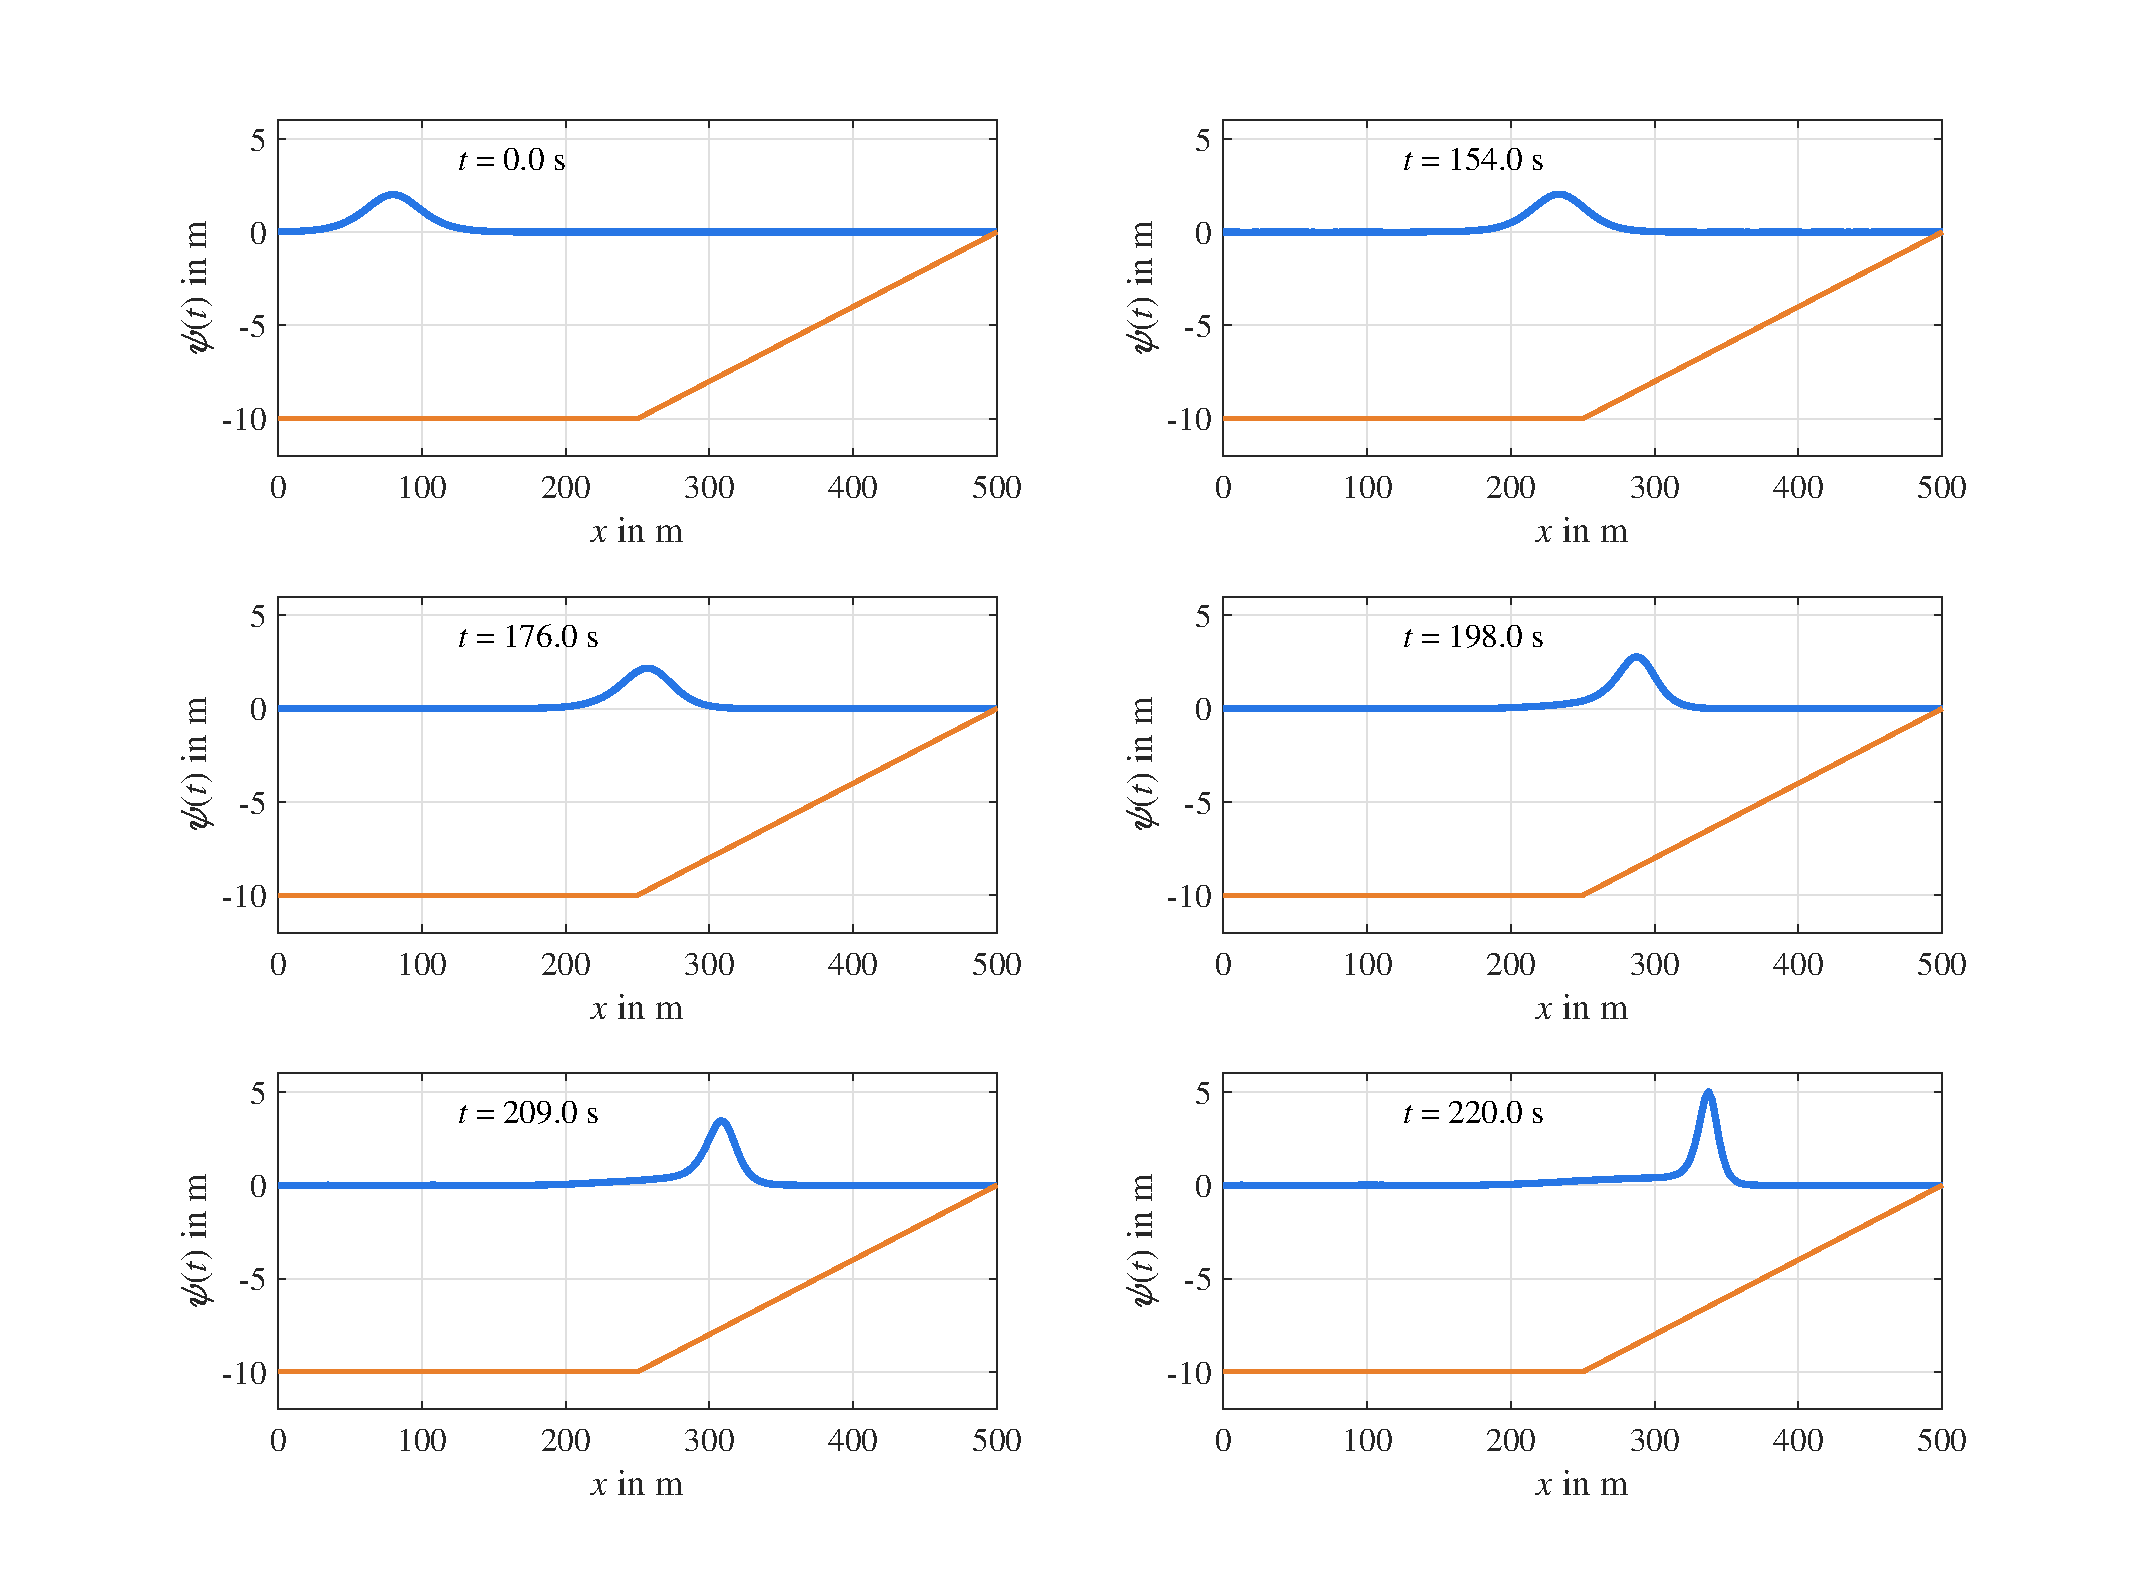
\includegraphics[width=\textwidth]{KdVTsunami.pdf}
    \caption[Eine Soliton-L�sung der Korteweg-de-Vries-Gleichung l�uft
    auf eine K�ste zu.]
    {Eine Soliton-L�sung der Korteweg-de-Vries-Gleichung aus einem Bereich mit
      einem Flachen Meeresgrund l�uft auf eine K�ste zu. Es entsteht nach und
      nach eine immer h�here St�rung der Wasseroberfl�che, die sich in Richtung
      der K�ste zu einer steilen Wand aufstellt.}
    \label{abb:kontmech_KdVTsumami}
  \end{figure}

  Die beispielhafte Rechnung geht von Salzwasser mit der Dichte von
  $\varrho = \SI{1020}{\kilo\gram\per\metre^3}$ und einer Oberfl�chenspannung
  von $T = \SI{0.07495}{\newton\per\metre}$ aus. Zun�chst hat das Wasser
  eine Tiefe von $d = \SI{10}{\metre}$, die schlie�lich auf Null abf�llt.
  Man erkennt, wie sich die Form des Solitons in K�stenn�he ver�ndert. Es
  wird h�her und verliert an Breite. Von der K�ste aus gesehen steigt es
  steil an. Hinter dem Maximum f�llt es wieder steil ab, jedoch gibt es einen
  flach auslaufenden Bereich. Blickt man von der K�ste aus auf ein solches
  Soliton, hat man den Eindruck, dass es sich zu einer Wand aufstellt.
\end{enumerate}

\end{sol} 
\textcolor{blue} {$\rightarrow$ zur} \probref{kontmech_tsunamis}.\\
\noindent\rule[1ex]{\textwidth}{0.5pt}  \newpage  \clearpage

% ----------------------------------------------------------------------------------------------------------
% ----------------------------------------------------------------------------------------------------------

 
%\clearpage
%\subsection{\mscre -- Physik des Kontinuums}\label{kap:kontmech_matlabskripts}

Die \mscre befinden sich im MATLAB-Ordner \texttt{MatlabDateien/kontmech},
die Hilfsfunktionen im dortigen Unterordner \texttt{Include\-folder} und Daten im Unterordner \texttt{Data}.
Es wird empfohlen, entweder die Skripte im GitHub Verzeichnis \githubSN zu benutzen oder sich die komplette Verzeichnisstruktur von \MKc~ runter zu laden und diese und auch das Arbeitsbuch im Hauptverzeichnis Fingeruebungen zu installieren. \\

Wir wollen noch einmal explizit darauf hinweisen, dass die \mscre prim�re der Vermittlung der physikalischen Modelle dienen und keinen Anspruch auf besonders elegante oder effiziente Programmierung erheben. Unser Buch ist ja kein Lehrbuch f�r \matlab-Programmierung. Uns ging es bewusst darum, dass die Skripte gut lesbar sind und das physikalische Modell bzw den physikalischen Gedankengang m�glichst klar abbilden.
Die Leser sind aufgerufen, die Programme nach Belieben zu verbessern und kompakter zu gestalten und diese auch ins GitHub Verzeichnis \githubSN zu stellen.


%\begin{prob}\label{mls:kontmech_hilfsfunktionen} %MLSkript1 
%\textbf{Hilfsfunktionen} \\
%\begin{longtable}{p{0.33\textwidth}p{0.67\textwidth}}
%\hline\noalign{\smallskip}
%Skript & Beschreibung \\
%\noalign{\smallskip}\svhline\noalign{\smallskip}
%Mathematische Funktionen \\
%\noalign{\smallskip}\svhline\noalign{\smallskip}
%\mlkontmechref{Beispiel.m} & Ein Beispieltext.\\
%\noalign{\smallskip}\svhline\noalign{\smallskip}
%\end{longtable}
%\end{prob}

\subsubsection {Skripte zu Beispielen} \label{mls:kontmech_kapitel} 
\begin{longtable}{p{0.33\textwidth}p{0.67\textwidth}}
\hline\noalign{\smallskip}
Skript & Beschreibung \\
\noalign{\smallskip}\svhline\noalign{\smallskip}
\mlkontmechref{SchwingendeSaite01.m} & L�sen der Differentialgleichung einer
schwingenden Saite f�r eine stehende Welle.\\
\noalign{\smallskip}\svhline\noalign{\smallskip}
\end{longtable}

\subsubsection {Skripte zu �bungen} \label{mls:kontmech_uebungen} 
\begin{longtable}{p{0.33\textwidth}p{0.67\textwidth}}
\hline\noalign{\smallskip}
Skript & Beschreibung \\
\noalign{\smallskip}\svhline\noalign{\smallskip}
\mlkontmechref{AchterbahnKont.m}        & L�sen der Differentialgleichung eines kontinuierlichen, elastischen Achterbahnzuges auf einer Gau�kurven-Strecke.\\
\mlkontmechref{AchterbahnKontBeschl.m}  & Normalbeschleunigung auf einen Fahrgast im kontinuierlichen, elastischen Achterbahnzug.\\
\mlkontmechref{Chladni01.m}             & L�sen der Eigenschwingungen einer kreisf�rmigen, elastischen Fl�che.\\
\mlkontmechref{Chladni02.m}             & L�sen der Eigenschwingungen einer quadratischen, elastischen Fl�che.\\
\mlkontmechref{Chladni03.m}             & L�sen der Eigenschwingungen einer rechteckigen, elastischen Fl�che.\\
\mlkontmechref{Divergenz.m}             & Programm berechnet Vektorfunktionen und ihre Divergenz.\\
\mlkontmechref{FassFormelGauss.m}       & Programm berechnet Volumen von Rotationsk�rpern �ber Gau�schen Integralsatz.\\
\mlkontmechref{GespannterBogen.m}       & L�sen der Eigenschwingungen eines Bogens, der durch eine Saite gespannt ist.\\
\mlkontmechref{GradientFunktion1.m}     & Programm berechnet Funktionen und ihre Gradienten.\\
\mlkontmechref{GradientFunktion2.m}     & Programm berechnet Funktionen und ihre Gradienten (Yukawa-Potential).\\
\mlkontmechref{GradientFunktion3.m}     & Programm berechnet Funktionen und ihre Gradienten (Kepler-Potential mit Drehimpuls).\\
\mlkontmechref{KdVTsunami.m}            & Berechnung eines KdV-Solitons, das auf eine K�ste zul�uft, an der die Wassertiefe abnimmt.\\
\mlkontmechref{KdV01.m}                 & L�sen der Korteweg-de-Vries-Gleichung f�r ein einzelnes Soliton.\\
\mlkontmechref{KdV02.m}                 & Vergleich mehrerer Solitonen der KdV-Gleichung mit unterschiedlicher Geschwindigkeit.\\
\mlkontmechref{KdV03.m}                 & Summen aus einzelnen Solitonen in der KdV-Gleichung.\\
\mlkontmechref{KdV04.m}                 & Interaktion von Solitonen in der KdV-Gleichung.\\
\mlkontmechref{Kreisrohr.m}             & Berechnen des Geschwindigkeitsprofils einer station�ren Str�mung in einem kreisrunden Rohr.\\
\mlkontmechref{NLSGSolitonen.m}         & L�sen der nichtlinearen Schr�dinger-Gleichung f�r ein Soliton.\\
\mlkontmechref{Rechteckrohr.m}          & Berechnen des Geschwindigkeitsprofils einer station�ren Str�mung in einem rechteckigen Rohr.\\
\mlkontmechref{Rotation.m}              & Programm berechnet Vektorfunktionen und ihre Rotation.\\
\mlkontmechref{SchwingendeSaite02.m}    & L�sen der Differentialgleichung einer eingespannten Saite f�r eine Gau�sche St�rung.\\
\mlkontmechref{SchwingendeSaite03.m}    & L�sen der Differentialgleichung einer eingespannten Saite f�r eine einseitig angeregte Welle.\\
%\noalign{\smallskip}\svhline\noalign{\smallskip}
\mlkontmechref{SinusGordonSolitonen.m}  & L�sen der Sinus-Gordon-Gleichung f�r ein Soliton.\\
\mlkontmechref{Tank.m}  & Fluss durch einen quadratischen Tank mit zwei �ffnungen.\\
\mlkontmechref{Torricelli.m}  & Fluss einer Fl�ssigkeit aus einem Tank nach dem
Gesetz von Torricelli.\\
\end{longtable}



 
%\clearpage
\renewcommand\glslongextraNameAlign{p{36mm}}
\renewcommand\glslongextraDescAlign{p{60mm}}
\clearpage
\bgroup
\small
\printunsrtglossary[type=kontmech]
\egroup
\clearpage
\fancyhead[RE]{\nouppercase\rightmark}
\bibliography{referenzen}
\clearpage
\fancyhead[RE]{\nouppercase\leftmark}
%%%%%%%%%%%%%%%%%%%%%%%%%%%%%%%%%%%%%%%%%%%%%%%%%%%%%%%%%%%%
%\input{footer.tex}
